\documentclass[11pt,oneside,openany]{book}
\usepackage[T1]{fontenc}
\usepackage[utf8]{inputenc}
\usepackage[spanish,es-noshorthands,es-tabla]{babel}
\usepackage{newpxtext}
\usepackage{newpxmath}
\unaccentedoperators
\usepackage{microtype}
\usepackage[a4paper,inner=2.5cm,outer=2.5cm,top=2.6cm,bottom=2.8cm,headsep=14pt]{geometry}
\usepackage{amsmath,mathtools}
\usepackage{booktabs,array,multirow,longtable,tabularx}
\usepackage{graphicx}
\usepackage[table]{xcolor}
\usepackage{enumitem}
\usepackage{fancyhdr}
\usepackage{titlesec}
\usepackage{caption}
\usepackage{subcaption}
\usepackage{tikz}
\usepackage{pgfplots}
\usepackage[most]{tcolorbox}
\usepackage{siunitx}
\usepackage{needspace}
\usepackage{listings}
\usepackage{xurl}
\usepackage{placeins}
\setlength{\headheight}{15pt}
\setlength{\emergencystretch}{1em}
\makeatletter
\renewcommand*\l@section{\@dottedtocline{1}{1.5em}{3.1em}}
\renewcommand*\l@subsection{\@dottedtocline{2}{4.6em}{3.2em}}
\makeatother

\pgfplotsset{compat=1.18}
\usetikzlibrary{arrows.meta,calc,positioning,patterns,decorations.pathmorphing,decorations.pathreplacing,shapes.geometric,shapes.misc,fit,backgrounds,shadings,matrix}
\usepgfplotslibrary{fillbetween,colormaps,statistics}
\sisetup{output-decimal-marker={,},group-separator={\,},group-minimum-digits=5,per-mode=symbol}

\definecolor{fuego}{HTML}{C8421C}
\definecolor{fuegoClaro}{HTML}{FBE6DC}
\definecolor{brasa}{HTML}{E08A1E}
\definecolor{brasaClaro}{HTML}{FCF0D8}
\definecolor{cielo}{HTML}{1F5A8A}
\definecolor{cieloClaro}{HTML}{E1ECF5}
\definecolor{bosque}{HTML}{2F6B3C}
\definecolor{bosqueClaro}{HTML}{E2F0E3}
\definecolor{violeta}{HTML}{5B3F8C}
\definecolor{violetaClaro}{HTML}{ECE6F5}
\definecolor{ceniza}{HTML}{4A4A4A}
\definecolor{cenizaClaro}{HTML}{EFEFEF}
\definecolor{modis}{HTML}{1F5A8A}
\definecolor{viirs}{HTML}{C8421C}

\captionsetup{font=small,labelfont={bf,color=cielo},margin=8mm}
\setlength{\parskip}{0.35em}
\setlist{itemsep=0.15em,topsep=0.3em}

\titleformat{\chapter}[display]
  {\normalfont\bfseries\color{cielo}}
  {\Large\MakeUppercase{\chaptertitlename}\ \thechapter}
  {8pt}
  {\Huge\color{black}}
  [\vspace{4pt}{\color{fuego}\titlerule[1.6pt]}]
\titleformat{\section}{\normalfont\Large\bfseries\color{cielo}}{\thesection}{0.8em}{}
\titleformat{\subsection}{\normalfont\large\bfseries\color{ceniza}}{\thesubsection}{0.8em}{}

\pagestyle{fancy}
\fancyhf{}
\fancyhead[L]{\small\color{ceniza}\nouppercase{\leftmark}}
\fancyhead[R]{\small\color{ceniza}\thepage}
\renewcommand{\headrulewidth}{0.4pt}
\fancypagestyle{plain}{\fancyhf{}\fancyfoot[C]{\small\thepage}\renewcommand{\headrulewidth}{0pt}}

\tcbset{cajalibro/.style={enhanced,breakable,boxrule=0pt,leftrule=3pt,arc=1.5pt,
  left=8pt,right=8pt,top=6pt,bottom=6pt,before skip=10pt,after skip=10pt,
  fonttitle=\bfseries\sffamily\small,coltitle=black,attach title to upper={\par\smallskip},
  parbox=false}}

\newtcolorbox{definicion}[1]{cajalibro,colback=cieloClaro,colframe=cielo,title={Definición: #1}}
\newtcolorbox{intuicion}[1][Intuición]{cajalibro,colback=brasaClaro,colframe=brasa,title={#1}}
\newtcolorbox{atencion}[1][Cuidado]{cajalibro,colback=fuegoClaro,colframe=fuego,title={#1}}
\newtcolorbox{parareto}[1][Para el reto]{cajalibro,colback=bosqueClaro,colframe=bosque,title={#1}}
\newtcolorbox{nota}[1][Nota]{cajalibro,colback=cenizaClaro,colframe=ceniza,title={#1}}

\newcounter{ejemplo}[chapter]
\renewcommand{\theejemplo}{\thechapter.\arabic{ejemplo}}
\newtcolorbox[use counter=ejemplo,number within=chapter]{ejemplo}[1]{cajalibro,colback=violetaClaro,colframe=violeta,
  title={Ejemplo \thetcbcounter: #1}}
\newcommand{\solucion}{\par\medskip\noindent\textbf{\sffamily\small Solución.}\ }

\newcommand{\objetivos}[1]{%
  \begin{tcolorbox}[cajalibro,colback=white,colframe=cielo,title={Al terminar este capítulo podrás}]
  #1
  \end{tcolorbox}}

\newcommand{\resumen}{\section*{Resumen del capítulo}\addcontentsline{toc}{section}{Resumen del capítulo}}
\newcommand{\ejercicios}{\section*{Ejercicios}\addcontentsline{toc}{section}{Ejercicios}}
\newcommand{\lecturas}{\section*{Para profundizar}\addcontentsline{toc}{section}{Para profundizar}}
\newcommand{\fuente}[1]{\textsuperscript{[\ref{src:#1}]}}

\newcommand{\um}{\si{\micro\metre}}
\newcommand{\termino}[1]{\textbf{\textit{#1}}}
\newcommand{\Tb}{T_{\mathrm{b}}}
\newcommand{\dd}{\,\mathrm{d}}

\lstset{basicstyle=\ttfamily\small,columns=fullflexible,frame=single,framerule=0.3pt,
  rulecolor=\color{ceniza!50},backgroundcolor=\color{cenizaClaro!60},breaklines=true,
  xleftmargin=6pt,xrightmargin=6pt,aboveskip=8pt,belowskip=8pt,
  literate={á}{{\'a}}1 {é}{{\'e}}1 {í}{{\'i}}1 {ó}{{\'o}}1 {ú}{{\'u}}1 {ñ}{{\~n}}1}

\tikzset{
  >={Stealth[length=2.2mm]},
  etiqueta/.style={font=\small},
  caja/.style={draw=ceniza,rounded corners=2pt,fill=white,align=center,font=\small,inner sep=5pt},
  flujo/.style={->,thick,color=ceniza},
}

\usepackage[colorlinks=true,linkcolor=cielo,urlcolor=fuego,citecolor=bosque]{hyperref}

\newcommand{\PeruFilas}{\num{1100073}}
\newcommand{\PeruAceptadas}{\num{908652}}
\newcommand{\PeruRatio}{\num{4.685}}
\newcommand{\PeruMAE}{\num{717.4}}
\newcommand{\PeruSesgo}{\num{115.4}}
\newcommand{\PeruWAPE}{\num{21.6}}
\newcommand{\PeruAjusteAqua}{\num{26508}}
\newcommand{\PeruAjusteVIIRS}{\num{124188}}
\newcommand{\PeruAgostoMediana}{\num{9444}}
\newcommand{\PeruAgostoActual}{\num{12447}}
\newcommand{\PeruAgostoAnomalia}{\num{31.8}}
\newcommand{\PeruSeptMediana}{\num{10967}}
\newcommand{\PeruSeptActual}{\num{15165}}
\newcommand{\PeruSeptQnoventa}{\num{13110.0}}
\newcommand{\PeruSeptAnomalia}{\num{38.3}}
\newcommand{\PeruASO}{\num{66.8}}

\newcommand{\PeruPotAlfa}{\num{27.4}}
\newcommand{\PeruPotBeta}{\num{0.75}}
\newcommand{\PeruPotWAPE}{\num{7.0}}
\newcommand{\PeruPotMAE}{\num{233.0}}
\newcommand{\PeruPotSesgo}{\num{28.8}}
\newcommand{\PeruRazonMin}{\num{3.4}}
\newcommand{\PeruRazonMax}{\num{11.4}}
\newcommand{\PeruCVUnica}{\num{32.6}}
\newcommand{\PeruTestUnica}{\num{21.6}}
\newcommand{\PeruAntesUnica}{\num{20.5}}
\newcommand{\PeruDespuesUnica}{\num{17.4}}
\newcommand{\PeruCVTrim}{\num{26.8}}
\newcommand{\PeruTestTrim}{\num{13.8}}
\newcommand{\PeruAntesTrim}{\num{12.4}}
\newcommand{\PeruDespuesTrim}{\num{12.9}}
\newcommand{\PeruCVMens}{\num{26.4}}
\newcommand{\PeruTestMens}{\num{17.5}}
\newcommand{\PeruAntesMens}{\num{15.1}}
\newcommand{\PeruDespuesMens}{\num{11.8}}
\newcommand{\PeruCVPot}{\num{16.6}}
\newcommand{\PeruTestPot}{\num{7.0}}
\newcommand{\PeruAntesPot}{\num{7.6}}
\newcommand{\PeruDespuesPot}{\num{12.0}}

\newcommand{\RegCostaAqua}{\num{1159}}
\newcommand{\RegCostaVIIRS}{\num{10130}}
\newcommand{\RegCostaRazon}{\num{8.74}}
\newcommand{\RegCostaAlfa}{\num{42.1}}
\newcommand{\RegCostaBeta}{\num{0.55}}
\newcommand{\RegCostaWapeUnica}{\num{26.4}}
\newcommand{\RegCostaWapePot}{\num{13.1}}
\newcommand{\RegSierraAqua}{\num{6498}}
\newcommand{\RegSierraVIIRS}{\num{32825}}
\newcommand{\RegSierraRazon}{\num{5.05}}
\newcommand{\RegSierraAlfa}{\num{22.1}}
\newcommand{\RegSierraBeta}{\num{0.73}}
\newcommand{\RegSierraWapeUnica}{\num{20.9}}
\newcommand{\RegSierraWapePot}{\num{16.2}}
\newcommand{\RegSelvaAqua}{\num{18851}}
\newcommand{\RegSelvaVIIRS}{\num{81233}}
\newcommand{\RegSelvaRazon}{\num{4.31}}
\newcommand{\RegSelvaAlfa}{\num{20.0}}
\newcommand{\RegSelvaBeta}{\num{0.77}}
\newcommand{\RegSelvaWapeUnica}{\num{19.8}}
\newcommand{\RegSelvaWapePot}{\num{8.5}}
\newcommand{\RegSumaUnica}{\num{17.6}}
\newcommand{\RegSumaPot}{\num{7.5}}

\newcommand{\NveinteRazon}{\num{0.964}}
\newcommand{\NveinteAjusteSNPP}{\num{125477}}
\newcommand{\NveinteAjusteNveinte}{\num{130144}}
\newcommand{\NveinteBeta}{\num{1.00}}
\newcommand{\NveinteAlfa}{\num{0.97}}
\newcommand{\NveinteWapeSin}{\num{7.6}}
\newcommand{\NveinteWapeRazon}{\num{6.5}}
\newcommand{\NveinteWapePot}{\num{6.5}}
\newcommand{\NveinteSesgoRazon}{\num{42.3}}
\newcommand{\NveinteTotalVeinticinco}{\num{29950}}
\newcommand{\NveinteConvVeinticinco}{\num{28876}}


\hypersetup{pdftitle={Fuego desde el espacio: teoría para armonizar los focos de calor de MODIS y VIIRS}}

\begin{document}

\frontmatter
\begin{titlepage}
\begin{tikzpicture}[remember picture,overlay]
  \fill[black!92] (current page.south west) rectangle (current page.north east);
  \begin{scope}[shift={($(current page.south)+(0,-9.5)$)}]
    \shade[inner color=cielo!70!black,outer color=black!92] (0,0) circle (16.5);
    \fill[cielo!35!black] (0,0) circle (15);
    \foreach \a/\r/\s in {78/14.6/0.10,84/14.2/0.07,88/14.75/0.12,93/14.4/0.08,97/14.7/0.10,
        102/14.1/0.06,106/14.55/0.09,81/14.85/0.07,91/14.9/0.06,99/14.3/0.11,110/14.7/0.07,
        73/14.5/0.08,86/14.6/0.05,95/14.85/0.08}{
      \shade[inner color=yellow!80!white,outer color=fuego,opacity=0.95] (\a:\r) circle (\s);
      \fill[fuego,opacity=0.18] (\a:\r) circle (3.2*\s);
    }
  \end{scope}
  \begin{scope}[shift={($(current page.north east)+(-5.2,-6.2)$)},rotate=-18]
    \fill[gray!35] (-0.5,-0.35) rectangle (0.5,0.35);
    \fill[cielo!60] (-2.1,-0.28) rectangle (-0.6,0.28);
    \fill[cielo!60] (0.6,-0.28) rectangle (2.1,0.28);
    \foreach \x in {-1.8,-1.5,-1.2,-0.9,0.9,1.2,1.5,1.8}{\draw[black!70,line width=0.3pt] (\x,-0.28)--(\x,0.28);}
    \fill[gray!60] (-0.12,-0.35) rectangle (0.12,-0.6);
  \end{scope}
  \coordinate (sat) at ($(current page.north east)+(-5.4,-6.75)$);
  \fill[brasa,opacity=0.10] (sat) -- ($(current page.south)+(-3.4,5.1)$) -- ($(current page.south)+(3.4,5.1)$) -- cycle;
  \draw[brasa,opacity=0.45,line width=0.4pt] (sat) -- ($(current page.south)+(-3.4,5.1)$) (sat) -- ($(current page.south)+(3.4,5.1)$);
  \node[anchor=north west,text=white,align=left,text width=14cm] at ($(current page.north west)+(2.2,-3.2)$) {%
    {\sffamily\bfseries\fontsize{40}{44}\selectfont\spaceskip=0.28em Fuego desde\\[2pt] el espacio\par}
    \vspace{10pt}
    {\color{brasa}\rule{7cm}{2pt}\par}
    \vspace{12pt}
    {\sffamily\Large Teoría para armonizar los focos de calor\\ de MODIS y VIIRS\par}
    \vspace{18pt}
    {\sffamily\normalsize\color{white!75!black} De la radiación de un cuerpo caliente\\ al calendario de quemas de una región\par}
  };
  \node[anchor=south west,text=white!80!black,align=left,font=\sffamily\small] at ($(current page.south west)+(2.2,2.0)$)
    {Libro de estudio para el reto\\[1pt]
    \textit{Harmonization of MODIS and VIIRS Hot Spots}\\[1pt]
    NASA Space Apps Challenge 2026 \textbullet\ Huancayo};
\end{tikzpicture}
\end{titlepage}

\tableofcontents
\chapter{Prefacio}

Este libro existe por una razón concreta: en pocos días hay que sentarse cuarenta y ocho horas
a construir una aplicación web que una dos registros satelitales de incendios, el de MODIS y el
de VIIRS, en un solo \emph{calendario de quemas}. La aplicación se puede programar sin entender
de dónde salen los datos, pero entonces cada decisión importante se toma a ciegas: qué contar,
qué descartar, por qué un sensor ve más fuego que el otro, cuánto confiar en el resultado. Y esas
decisiones son justamente las que un jurado va a preguntar.

Por eso el libro no es una lista de enlaces ni un resumen. Es un recorrido completo, pensado
para leerse de principio a fin, que parte de una pregunta física muy simple (¿por qué brilla
algo caliente?) y termina en preguntas de diseño (¿qué número le muestro a un bombero?). Cada
capítulo se apoya en los anteriores.

\section*{Cómo está organizado}

\begin{description}[leftmargin=1.2em,style=nextline]
  \item[Parte I. El fuego y la luz.] Qué es un foco de calor, cómo emite radiación un cuerpo
  caliente y qué le pasa a esa radiación al cruzar la atmósfera. Es la física mínima para
  entender por qué un incendio de cien metros cuadrados puede verse desde 700 km de altura.
  \item[Parte II. Satélites y sensores.] Cómo se mueven los satélites, por qué pasan siempre a
  la misma hora, cómo barren el suelo y en qué se diferencian MODIS y VIIRS como instrumentos.
  \item[Parte III. Del píxel al foco de calor.] El algoritmo que decide si un píxel tiene fuego,
  la potencia radiativa del fuego, los errores del sistema y el formato exacto de los datos que
  entrega FIRMS.
  \item[Parte IV. Armonizar dos registros.] La estadística necesaria, las estrategias para
  volver comparables los dos sensores y la construcción del calendario de quemas con sus
  anomalías.
  \item[Parte V. Hacia la aplicación.] Cómo procesar millones de puntos con rapidez y cómo se
  traduce todo lo anterior en una herramienta para Junín y el Perú.
\end{description}

\section*{Cómo leerlo}

Cada capítulo abre con sus objetivos y cierra con un resumen, una lista de ejercicios y lecturas
para profundizar. Los resúmenes están al final a propósito: sirven para repasar, no para
reemplazar la lectura. A lo largo del texto aparecen cajas de colores con una función fija:

\begin{definicion}{término nuevo}
Las cajas azules fijan el significado exacto de un término la primera vez que aparece.
\end{definicion}

\begin{intuicion}
Las cajas ámbar dan una imagen mental o una analogía para una idea difícil.
\end{intuicion}

\begin{ejemplo}{así se ven los ejemplos resueltos}
Las cajas violetas plantean un problema con números y lo resuelven paso a paso.
\solucion Conviene tapar la solución e intentarlo antes de leerla.
\end{ejemplo}

\begin{atencion}
Las cajas rojas marcan errores frecuentes y trampas de los datos.
\end{atencion}

\begin{parareto}
Las cajas verdes conectan la teoría con decisiones concretas del proyecto.
\end{parareto}

\section*{Sobre los números y las figuras}

Los ejemplos de radiancias, temperaturas de brillo y periodos orbitales se calculan
con las fórmulas del libro. Los esquemas y ciertos ejercicios estadísticos usan números
didácticos, identificados como tales. En cambio, el calendario introductorio y los
casos de los capítulos~\ref{cap:calendario} y~\ref{cap:aplicacion} usan \textbf{datos reales
de Perú}: 24 archivos anuales de NASA FIRMS, con sus originales, procedencia y programas
de cálculo. Las escenas del Camp Fire y de la selva peruana son imágenes reales de
NASA Worldview; sus pies explican qué se observa y qué no puede deducirse del color.
Las referencias están en el apéndice~\ref{ap:fuentes}.

La edición continuada el 9 de noviembre de 2026 completa los catorce capítulos y sus
tres apéndices. También actualiza el estado de Suomi NPP y matiza supuestos de cobertura,
agregación y validación. Un libro terminado sigue distinguiendo una demostración
reproducible de un producto científico validado para uso operativo.

\section*{Una advertencia honesta}

Los recursos oficiales del reto se publican el día anterior al hackathon. Es posible que
propongan una definición particular de <<actividad de quema>> o un método de armonización
preferido. Si eso ocurre, lo que diga el enunciado manda sobre lo que diga este libro; la teoría
de aquí es la base para entender y aplicar con criterio lo que pidan.


\mainmatter

\part{El fuego y la luz}
\chapter{Un registro partido en dos}\label{cap:problema}

\objetivos{
\begin{itemize}
  \item Explicar qué es y qué no es un foco de calor satelital.
  \item Describir por qué el registro mundial de focos está repartido entre dos familias de
  sensores y por qué no se pueden sumar directamente.
  \item Enunciar con tus propias palabras qué significa <<armonizar>> y qué es un calendario de
  quemas.
  \item Ubicar cada capítulo del libro dentro del problema completo.
\end{itemize}}

\section{El fuego como fenómeno del planeta}

Cada año arde en la Tierra una superficie del orden de varios millones de kilómetros
cuadrados. La mayor parte no son los grandes incendios que salen en las noticias, sino fuegos
pequeños y repetidos: pastos que se queman para que rebroten, rastrojos que se eliminan después
de la cosecha, parcelas que se abren en el bosque. A todo ese conjunto se le llama
\termino{quema de biomasa}.

El fuego tiene estaciones. En cada región hay meses en los que casi nunca arde nada y meses en
los que arde casi todos los días, y ese ritmo depende del clima (cuándo termina la lluvia y la
vegetación se seca) y de las personas (cuándo se cosecha, cuándo se prepara la tierra). En la
sierra del Perú, por ejemplo, las quemas agrícolas se concentran al final de la estación seca,
y la mayor parte de los incendios forestales reportados ocurre entre agosto y septiembre, casi
siempre porque una quema agrícola se salió de control.

Conocer ese ritmo sirve para cosas muy prácticas: saber en qué semanas hay que tener brigadas
listas, distinguir un año normal de uno excepcional, o evaluar si una política de prohibición
de quemas tuvo algún efecto. Pero nadie puede recorrer un país entero contando fuegos. La única
forma de observar el fuego en todas partes y todos los días es desde el espacio.

\section{Qué es un foco de calor}

Un satélite de observación no toma una fotografía en el sentido habitual. Mide, para cada
pequeña porción del suelo, cuánta radiación llega al sensor en ciertas longitudes de onda. Cada
una de esas porciones es un \termino{píxel}. Un píxel de MODIS cubre aproximadamente un
kilómetro cuadrado; uno de VIIRS, unos 375 metros de lado.

\begin{definicion}{foco de calor (hot spot)}
Un foco de calor, o \emph{detección de fuego activo}, es un píxel que un algoritmo ha
clasificado como <<contiene fuego en el momento de la observación>>, porque emite en el
infrarrojo mucha más radiación que los píxeles que lo rodean. El dato que se publica es el
\textbf{centro del píxel}, con su fecha, su hora y algunas medidas adicionales.
\end{definicion}

La definición tiene tres consecuencias que conviene grabar desde el principio, porque todo el
problema de la armonización nace de ellas.

\textbf{Un foco no es un incendio.} Un incendio grande puede ocupar decenas de píxeles a la vez
y durar varios días, de modo que genera cientos de focos. Y al revés: varias quemas pequeñas
dentro del mismo píxel generan un solo foco. La relación entre <<número de focos>> y <<número
de incendios>> no es fija.

\textbf{Un foco no dice dónde está el fuego, sino en qué píxel está.} La coordenada publicada es
el centro del píxel. El fuego puede estar en cualquier punto dentro de él, y con un píxel de un
kilómetro eso significa una incertidumbre de varios cientos de metros
(figura~\ref{fig:foco-pixel}).

\textbf{Un foco es una observación instantánea.} El satélite pasa, mira durante una fracción de
segundo y se va. Si el fuego empezó después o se apagó antes, no queda registrado. Si había una
nube encima, tampoco.

\begin{figure}[ht]
\centering
\begin{tikzpicture}[scale=0.95]
  \begin{scope}
    \fill[bosque!25] (0,0) rectangle (6,6);
    \fill[bosque!40] (0.4,3.4) to[bend left=25] (2.6,5.6) to[bend left=30] (3.4,3.2) to[bend left=20] cycle;
    \fill[brasa!30] (3.5,0.4) rectangle (5.6,2.2);
    \foreach \x in {0,2,4,6}{\draw[ceniza,thin] (\x,0)--(\x,6); \draw[ceniza,thin] (0,\x)--(6,\x);}
    \shade[inner color=yellow,outer color=fuego] (4.55,4.75) circle (0.16);
    \shade[inner color=yellow,outer color=fuego] (4.8,4.4) circle (0.09);
    \shade[inner color=yellow,outer color=fuego] (2.5,1.3) circle (0.11);
    \node[font=\small\bfseries] at (3,6.45) {Lo que hay en el suelo};
    \draw[<->] (0,-0.35)--(2,-0.35) node[midway,below,font=\footnotesize]{1 km};
  \end{scope}
  \draw[->,very thick,ceniza] (6.5,3)--(7.9,3) node[midway,above,font=\footnotesize]{sensor};
  \begin{scope}[shift={(8.4,0)}]
    \fill[cenizaClaro] (0,0) rectangle (6,6);
    \fill[fuego!55] (4,4) rectangle (6,6);
    \fill[fuego!55] (2,0) rectangle (4,2);
    \foreach \x in {0,2,4,6}{\draw[ceniza,thin] (\x,0)--(\x,6); \draw[ceniza,thin] (0,\x)--(6,\x);}
    \fill[black] (5,5) circle (0.09) node[below=2pt,font=\footnotesize]{foco};
    \fill[black] (3,1) circle (0.09) node[below=2pt,font=\footnotesize]{foco};
    \node[font=\small\bfseries] at (3,6.45) {Lo que queda en los datos};
  \end{scope}
\end{tikzpicture}
\caption{Del terreno al dato. A la izquierda, tres fuegos reales de distinto tamaño sobre una
cuadrícula de píxeles. A la derecha, lo que publica el sistema: dos puntos, cada uno en el
centro de un píxel. Los dos fuegos que comparten píxel se convierten en un solo foco, y
ninguna coordenada coincide con la posición real de las llamas.}
\label{fig:foco-pixel}
\end{figure}

\begin{ejemplo}{focos frente a incendios}
Un incendio de pastizal avanza durante tres días con un frente de unos 4 km de largo. Un sensor
con píxeles de 1 km lo observa dos veces al día. ¿Cuántos focos produce, aproximadamente?
¿Y si en esos mismos tres días un agricultor quema un rastrojo de 30 m por 30 m durante una
hora, a las 9 de la mañana, y el satélite pasa a las 13:30?
\solucion El frente de 4 km cruza unos 4 píxeles en cada pasada. Con dos pasadas diarias
durante tres días se obtienen alrededor de $4 \times 2 \times 3 = 24$ focos, todos del mismo
incendio. La quema del agricultor produce \textbf{cero} focos: cuando el satélite pasa, lleva
horas apagada. En los datos, el primer evento pesa 24 y el segundo no existe, aunque en el
terreno ambos fueron <<un fuego>>.
\end{ejemplo}

\section{Un caso real: el foco frente al fuego}

La figura~\ref{fig:foco-pixel} es un esquema. La figura~\ref{fig:camp} muestra lo mismo con
datos reales: el incendio \emph{Camp Fire}, en el norte de California, observado por VIIRS
(satélite Suomi NPP) el 9 de noviembre de 2018, un día después de iniciarse. Se eligió este
caso porque el cielo estaba despejado y el frente de fuego se distingue con claridad. El
recuadro mide unos 65~km de norte a sur.

\begin{figure}[ht]
\centering
\begin{subfigure}{0.32\textwidth}
  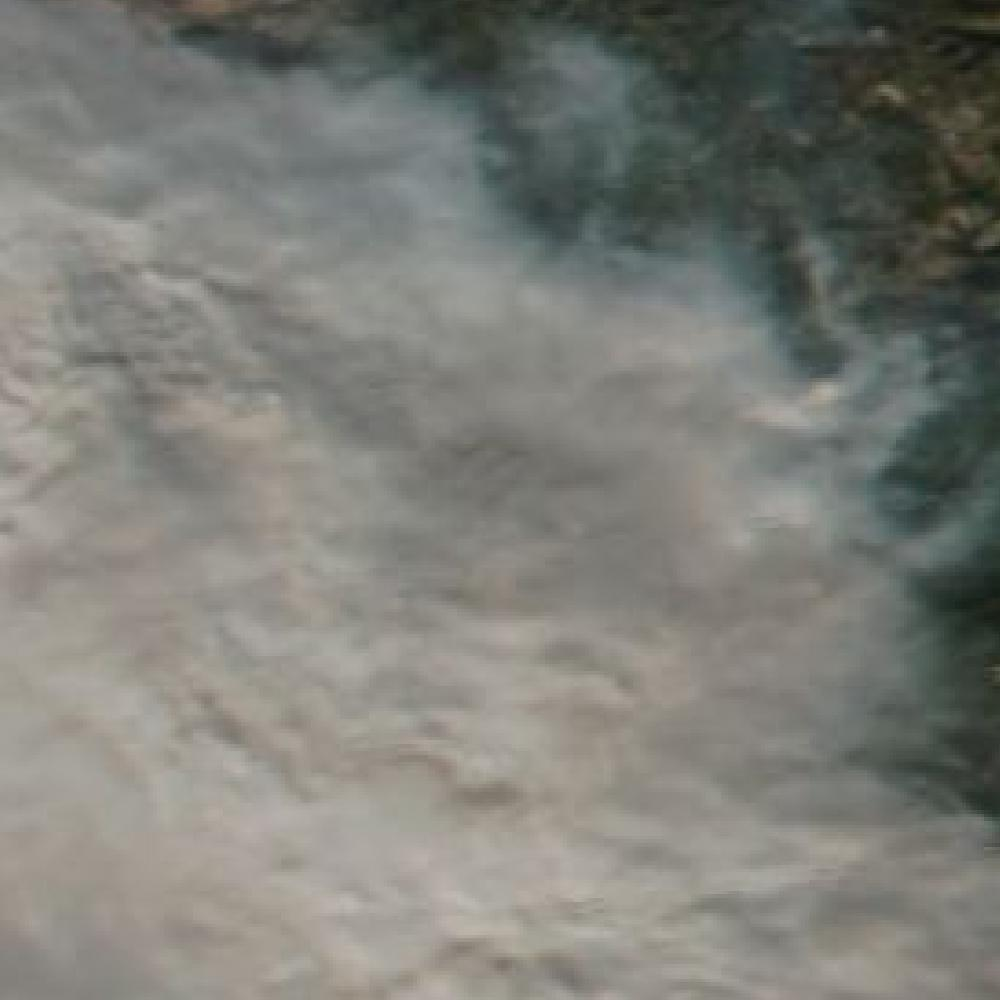
\includegraphics[width=\linewidth]{figuras/camp_color.jpg}
  \caption{Color verdadero: lo que vería el ojo.}
\end{subfigure}\hfill
\begin{subfigure}{0.32\textwidth}
  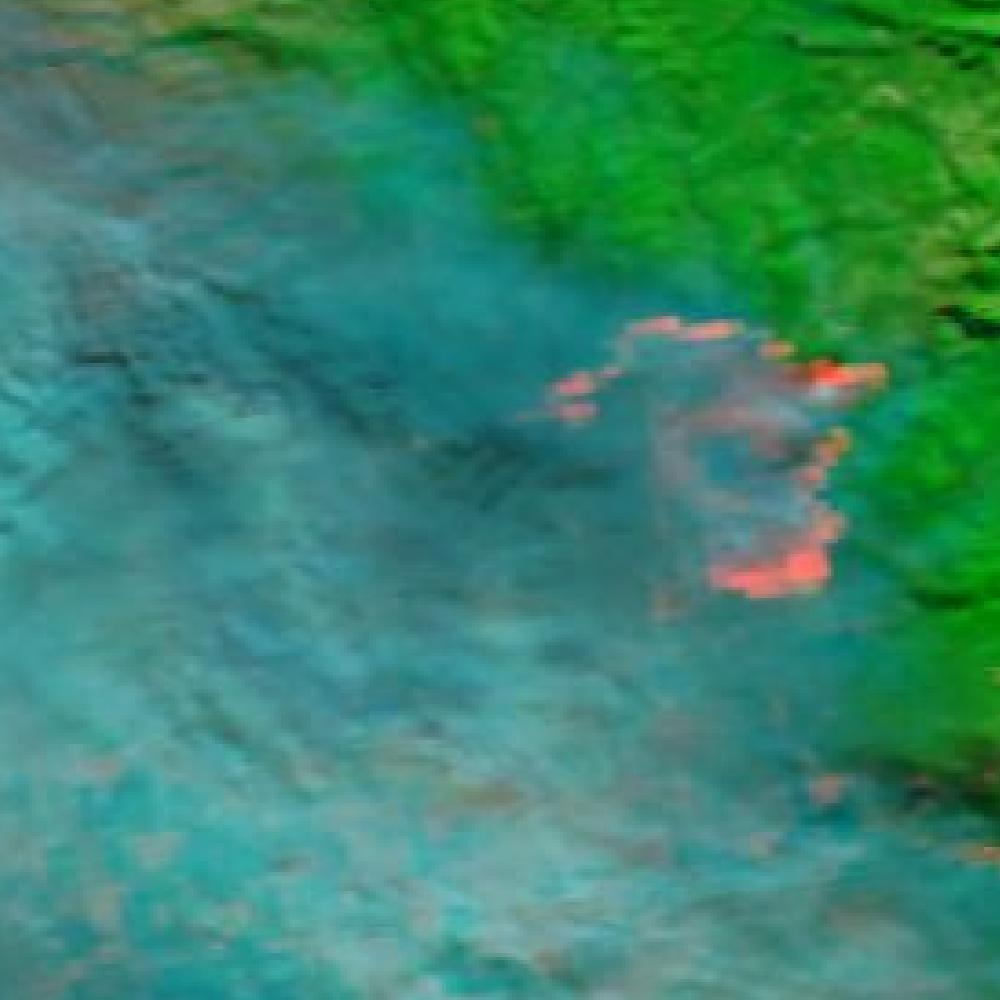
\includegraphics[width=\linewidth]{figuras/camp_falso.jpg}
  \caption{Falso color con infrarrojo de onda corta.}
\end{subfigure}\hfill
\begin{subfigure}{0.32\textwidth}
  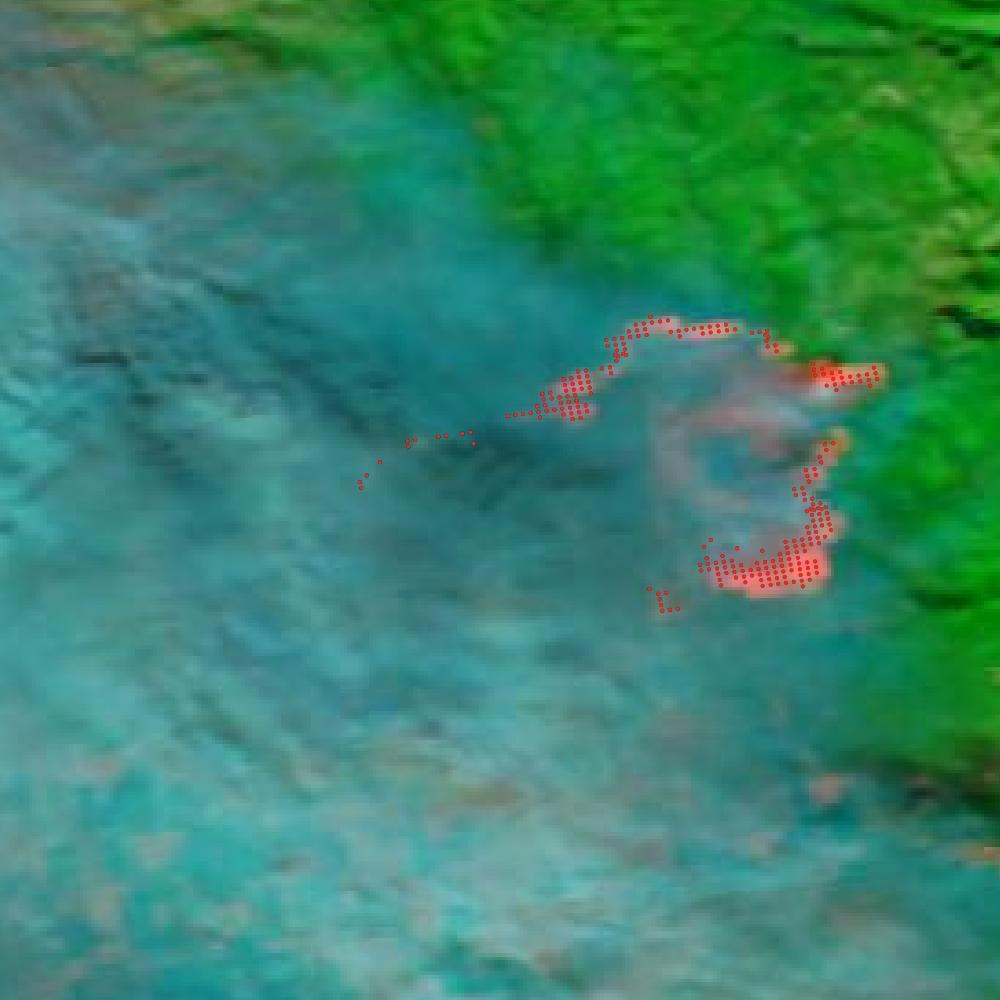
\includegraphics[width=\linewidth]{figuras/camp_focos.jpg}
  \caption{La misma imagen con los focos de 375~m.}
\end{subfigure}

\medskip
\begin{tikzpicture}
  \node[inner sep=0,anchor=south west] (z) at (0,0) {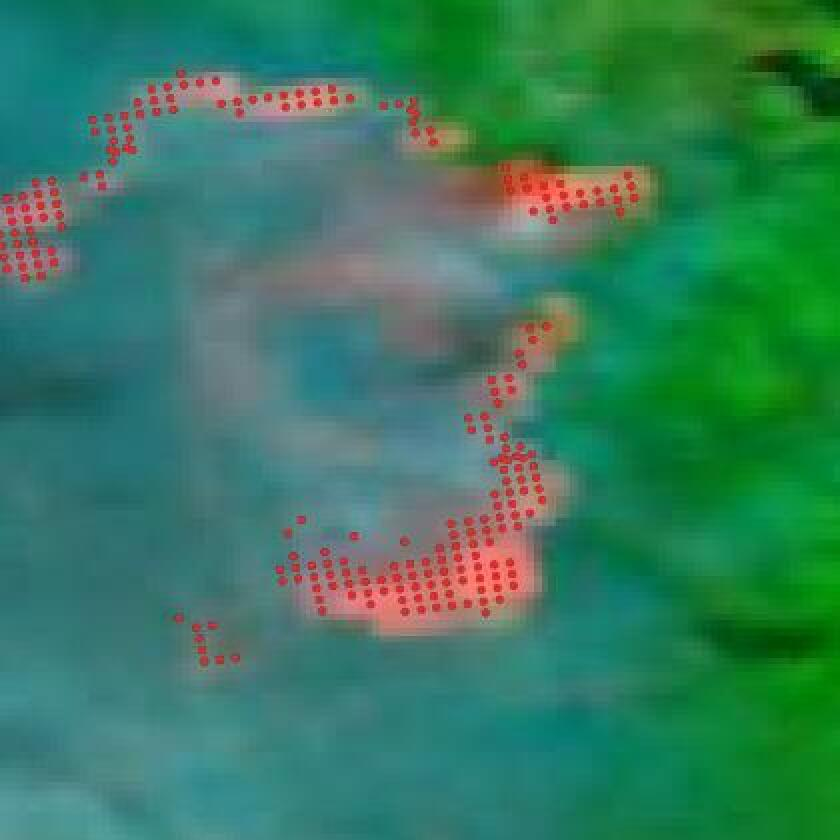
\includegraphics[width=0.5\textwidth]{figuras/camp_zoom.jpg}};
  \node[anchor=west,text width=0.42\textwidth,align=left,font=\small] at ($(z.east)+(0.5,0)$) {%
    \textbf{(d) Ampliación del panel (c).}\\[4pt]
    Cada punto rojo es un foco: el centro de un píxel clasificado como fuego.\\[4pt]
    Los puntos forman una \textbf{rejilla regular}. Esa rejilla no es la forma del incendio: es
    la cuadrícula de píxeles del sensor.\\[4pt]
    El frente continuo de llamas (en naranja brillante) queda convertido en una colección de
    puntos sueltos.};
\end{tikzpicture}
\caption{Un incendio real y sus focos de calor: \emph{Camp Fire}, California, 9 de noviembre de
2018. Imágenes de VIIRS/Suomi NPP obtenidas de NASA Worldview: (a) reflectancia corregida en
color verdadero; (b) combinación de bandas M11--I2--I1; (c) y (d) la misma combinación con la
capa de anomalías térmicas de 375~m.}
\label{fig:camp}
\end{figure}

Los cuatro paneles enseñan cosas distintas.

\textbf{(a) En el visible solo se ve humo.} Una columna densa cubre casi todo el recuadro y
oculta por completo dónde están las llamas.

\textbf{(b) En el infrarrojo se ve el fuego.} Esta combinación asigna al color rojo una banda
del infrarrojo de onda corta (2,25~\um), en la que las superficies muy calientes emiten con
fuerza y que el humo deja pasar. El frente activo aparece como un anillo naranja brillante, el
bosque sano en verde y el humo en tonos azulados y translúcidos. Es una comprobación visual de
lo que explicará el capítulo~\ref{cap:atmosfera}: el infrarrojo atraviesa el humo.

\textbf{(c) y (d) Los focos son la versión digital de ese anillo.} Cada píxel de 375~m del
frente que superó las pruebas del algoritmo se convierte en un punto. En la ampliación se
aprecia que los puntos están alineados en filas y columnas: son centros de píxeles, no
posiciones de llamas.

Este único incendio produjo, en esta sola pasada, un gran número de focos; una quema agrícola
produce uno o ninguno. Quien cuente focos sin pensar en esto estará midiendo sobre todo el
tamaño de los incendios más grandes, y casi nada de los pequeños.

\section{Dos familias de sensores}

Los focos de calor que distribuye la NASA provienen de dos instrumentos.

\termino{MODIS} (\emph{Moderate Resolution Imaging Spectroradiometer}) vuela en dos satélites:
Terra, lanzado a fines de 1999, y Aqua, lanzado en 2002. Su registro de focos empieza en
noviembre de 2000 y es el más largo que existe con cobertura global diaria. Sus píxeles de
fuego miden 1 km en el punto situado justo debajo del satélite.

\termino{VIIRS} (\emph{Visible Infrared Imaging Radiometer Suite}) es su sucesor. Vuela en el
satélite Suomi NPP desde fines de 2011, en NOAA-20 desde fines de 2017 y en NOAA-21 desde fines
de 2022. Su producto principal de focos usa píxeles de 375 m.

La figura~\ref{fig:cronologia} resume el solape disponible. La continuidad exige enlazar
sensores y plataformas, y revisar cambios de procesamiento y hora de paso. Las fechas
se refieren al archivo de focos, no necesariamente al lanzamiento del satélite.

\begin{figure}[ht]
\centering
\begin{tikzpicture}[x=0.43cm,y=0.65cm]
  \draw[->,thick] (0,0)--(28.5,0);
  \foreach \a in {2000,2004,2008,2012,2016,2020,2024}{
    \pgfmathsetmacro{\x}{\a-2000}
    \draw (\x,.12)--(\x,-.12) node[below,font=\footnotesize]{\a};
  }
  \fill[modis!85] (.85,5) rectangle (26.85,5.6);\node[left,font=\small] at (.6,5.3){Terra};
  \fill[modis!60] (2.5,4) rectangle (26.85,4.6);\node[left,font=\small] at (.6,4.3){Aqua};
  \fill[viirs!85] (12.05,2.6) rectangle (26.84,3.2);\node[left,font=\small] at (.6,2.9){Suomi NPP};
  \fill[viirs!65] (18.25,1.6) rectangle (26.85,2.2);\node[left,font=\small] at (.6,1.9){NOAA-20};
  \fill[viirs!45] (23.16,.6) rectangle (26.85,1.2);\node[left,font=\small] at (.6,.9){NOAA-21};
  \draw[dashed,ceniza] (26.85,-.2)--(26.85,6);
  \node[font=\footnotesize,anchor=south east] at (26.85,6){consulta: noviembre de 2026};
  \node[font=\footnotesize,align=center] at (19,-1.3){solape entre plataformas:\\base para comparar sus registros};
\end{tikzpicture}
\caption{Cronología del archivo FIRMS, consultada el 9 de noviembre de 2026. Las barras
se cortan en la fecha de consulta y no predicen el fin de las misiones. Suomi NPP cerró
su entrega el 2 de noviembre de 2026; NOAA-21 figura en el archivo desde marzo de 2023.
Se omiten interrupciones internas. Fuentes: NASA FIRMS y NOAA.\fuente{firms-archive}\fuente{noaa-snpp}}
\label{fig:cronologia}
\end{figure}

\section{Por qué no se pueden sumar}

Imagina que quieres responder una pregunta sencilla: \emph{¿está ardiendo más mi región ahora
que hace veinte años?} Lo natural sería contar los focos de cada año y dibujar la serie. Si lo
haces mezclando sensores, obtienes algo parecido a la figura~\ref{fig:salto}: una serie que da
un salto enorme justo cuando entra VIIRS.

\begin{figure}[ht]
\centering
\begin{tikzpicture}
\begin{axis}[width=13cm,height=6.2cm,ybar,bar width=7pt,
  xlabel={Año},ylabel={Focos por año},ymin=0,ymax=5200,
  xtick={2002,2006,2010,2014,2018,2022},x tick label style={/pgf/number format/1000 sep=},
  scaled y ticks=false,y tick label style={/pgf/number format/1000 sep={\,}},
  legend style={at={(0.5,1.03)},anchor=south,font=\small,draw=none,fill=none,legend columns=2,/tikz/every even column/.append style={column sep=10pt}},
  axis lines*=left,ymajorgrids,grid style={ceniza!20}]
\addplot[fill=modis!80,draw=none] coordinates {(2001,820)(2002,910)(2003,1040)(2004,870)(2005,1260)
 (2006,930)(2007,1110)(2008,880)(2009,960)(2010,1320)(2011,900)};
\addplot[fill=viirs!80,draw=none] coordinates {(2012,3650)(2013,3320)(2014,3480)(2015,3900)(2016,4480)
 (2017,3610)(2018,3540)(2019,3820)(2020,4390)(2021,3700)(2022,3950)(2023,4100)(2024,4750)};
\legend{MODIS,VIIRS}
\draw[<-,thick,ceniza] (axis cs:2011.6,2500)--(axis cs:2008.2,3600)
  node[left,font=\small,align=right,text=black]{¿Se cuadruplicó el fuego\\ en un solo año?};
\end{axis}
\end{tikzpicture}
\caption{Lo que ocurre si se cambia de sensor sin corregir (datos ilustrativos). El salto de
2012 no es un cambio en el fuego: es un cambio en el instrumento con que se lo mira.}
\label{fig:salto}
\end{figure}

El salto es un artefacto. VIIRS detecta más focos que MODIS mirando exactamente los mismos
fuegos, por varias razones que el libro irá desarmando una por una:

\begin{itemize}
  \item Sus píxeles son más pequeños, así que un fuego chico destaca más contra su fondo y es
  detectado, mientras que en un píxel grande de MODIS queda diluido
  (capítulos~\ref{cap:radiacion} y~\ref{cap:deteccion}).
  \item Un mismo incendio ocupa más píxeles pequeños que píxeles grandes, de modo que genera
  más focos aunque los dos sensores lo vean entero.
  \item Sus píxeles crecen mucho menos hacia los bordes de la imagen
  (capítulo~\ref{cap:escaneo}).
  \item Su franja de observación es más ancha y no deja huecos entre órbitas cerca del ecuador
  (capítulo~\ref{cap:orbitas}).
  \item El número de satélites en vuelo ha ido cambiando: uno, dos, tres.
\end{itemize}

\begin{intuicion}[Analogía: dos termómetros]
Supón que una estación meteorológica midió la temperatura durante doce años con un termómetro
viejo que marca dos grados de menos, y luego lo cambió por uno nuevo y exacto. Si unes las dos
series tal cual, <<descubres>> un calentamiento brusco de dos grados el día del cambio. Nadie
aceptaría esa conclusión. Lo correcto es tener ambos termómetros funcionando juntos durante un
tiempo, medir cuánto difieren y corregir una de las series. Eso mismo, con focos en lugar de
grados, es armonizar.
\end{intuicion}

\section{Qué significa armonizar}

\begin{definicion}{armonización}
Armonizar dos registros es transformarlos para que midan la misma cantidad en la misma escala,
de modo que las diferencias que queden entre ellos reflejen cambios del fenómeno observado y no
diferencias entre instrumentos.
\end{definicion}

La armonización es posible gracias al periodo de solape de la figura~\ref{fig:cronologia}.
Desde 2012 ambos sensores observan los mismos lugares, muchas veces con pocos minutos de
diferencia. Esos años permiten \emph{aprender} la relación entre lo que ve uno y lo que ve el
otro, y aplicarla después a los años en que solo existe uno de los dos.

Hay tres preguntas que cualquier método de armonización debe responder, y el libro dedica un
capítulo a cada una:

\begin{enumerate}
  \item \textbf{¿Qué se cuenta?} No es obvio que la unidad correcta sea <<un foco>>. Puede ser
  más robusto contar <<días con fuego en una celda>> (capítulo~\ref{cap:armonizacion}).
  \item \textbf{¿Cómo se relacionan los dos sensores?} Un factor constante, una recta, una
  relación distinta por región y por mes (capítulos~\ref{cap:estadistica}
  y~\ref{cap:armonizacion}).
  \item \textbf{¿Cuánto confiar en el resultado?} Toda corrección tiene incertidumbre y hay que
  saber medirla y mostrarla (capítulo~\ref{cap:estadistica}).
\end{enumerate}

\section{El calendario de quemas}

El producto final que pide el reto no es la serie armonizada en sí, sino una forma de leerla.

\begin{definicion}{calendario de quemas}
Un calendario de quemas es un resumen, para un área elegida, de \textbf{cuándo} arde a lo largo
del año: en qué semanas o meses se concentra históricamente la actividad, cuánta es normal en
cada época y qué periodos concretos se salieron de lo normal.
\end{definicion}

La figura~\ref{fig:calendario-intro} muestra una de sus formas más habituales: una matriz con
los años en un eje y los meses en el otro, coloreada según la actividad. De un vistazo se
reconocen la temporada (la banda vertical más oscura) y los años excepcionales (las filas que
destacan). El capítulo~\ref{cap:calendario} explica cómo se construye y cómo se definen con
rigor <<normal>> y <<excepcional>>.

\begin{figure}[ht]
\centering
\begin{tikzpicture}
\begin{axis}[width=13cm,height=6.7cm,xmin=.5,xmax=12.5,ymin=-.5,ymax=11.5,y dir=reverse,
 xtick={1,...,12},xticklabels={E,F,M,A,M,J,J,A,S,O,N,D},
 ytick={0,2,4,6,8,10,11},yticklabels={2013,2015,2017,2019,2021,2023,2024},
 colormap={peruintro}{color(0cm)=(white);color(1cm)=(brasaClaro);color(2cm)=(fuego)},
 colorbar,colorbar style={ylabel={Celdas-día},scaled ticks=false,tick label style={font=\scriptsize}}]
\addplot[matrix plot*,mesh/cols=12,point meta=explicit,draw=white,line width=.2pt]
 table[x=mes,y=fila,meta=actividad,col sep=comma]{datos/peru_calendario.csv};
\end{axis}
\end{tikzpicture}
\caption{Calendario con \textbf{datos reales de Perú}: VIIRS/Suomi NPP, 2013--2024,
solo detecciones diurnas tipo 0 y de confianza nominal/alta, agrupadas por celda de
$0{,}05^\circ$ y día. Fuente: NASA FIRMS; cálculo propio. Los filtros, las limitaciones
y la comparación estacional se desarrollan en el capítulo~\ref{cap:calendario}.}
\label{fig:calendario-intro}
\end{figure}

\section{El mapa del libro}

La figura~\ref{fig:mapa} resume el camino completo, desde las llamas hasta el número que ve el
usuario. Cada flecha es una transformación que introduce supuestos y errores, y cada una se
estudia en un capítulo. Entender la cadena entera es lo que permite decidir con criterio en el
último eslabón.

\begin{figure}[ht]
\centering
\begin{tikzpicture}[node distance=5mm and 7mm]
  \node[caja,fill=fuegoClaro] (a) {Fuego\\ en el suelo};
  \node[caja,right=of a,fill=brasaClaro] (b) {Radiación\\ infrarroja};
  \node[caja,right=of b,fill=cieloClaro] (c) {Atmósfera};
  \node[caja,right=of c,fill=cieloClaro] (d) {Sensor\\ en órbita};
  \node[caja,right=of d,fill=violetaClaro] (e) {Píxel y\\ algoritmo};
  \node[caja,below=12mm of e,fill=violetaClaro] (f) {Foco de calor\\ (FIRMS)};
  \node[caja,left=of f,fill=bosqueClaro] (g) {Conteo en\\ celdas y días};
  \node[caja,left=of g,fill=bosqueClaro] (h) {Serie\\ armonizada};
  \node[caja,left=of h,fill=bosqueClaro] (i) {Calendario\\ y anomalías};
  \node[caja,left=of i,fill=white] (j) {Decisión\\ del usuario};
  \draw[flujo] (a)--(b); \draw[flujo] (b)--(c); \draw[flujo] (c)--(d); \draw[flujo] (d)--(e);
  \draw[flujo] (e)--(f); \draw[flujo] (f)--(g); \draw[flujo] (g)--(h); \draw[flujo] (h)--(i); \draw[flujo] (i)--(j);
  \node[font=\footnotesize,ceniza,above=1mm of b] {cap.~\ref{cap:radiacion}};
  \node[font=\footnotesize,ceniza,above=1mm of c] {cap.~\ref{cap:atmosfera}};
  \node[font=\footnotesize,ceniza,above=1mm of d] {caps.~\ref{cap:orbitas}--\ref{cap:modisviirs}};
  \node[font=\footnotesize,ceniza,above=1mm of e] {caps.~\ref{cap:deteccion}--\ref{cap:errores}};
  \node[font=\footnotesize,ceniza,below=1mm of f] {cap.~\ref{cap:firms}};
  \node[font=\footnotesize,ceniza,below=1mm of g] {caps.~\ref{cap:armonizacion},~\ref{cap:aplicacion}};
  \node[font=\footnotesize,ceniza,below=1mm of h] {caps.~\ref{cap:estadistica},~\ref{cap:armonizacion}};
  \node[font=\footnotesize,ceniza,below=1mm of i] {cap.~\ref{cap:calendario}};
\end{tikzpicture}
\caption{La cadena completa, de las llamas a la decisión, y el capítulo que estudia cada
eslabón.}
\label{fig:mapa}
\end{figure}

\resumen

\begin{itemize}
  \item Un \textbf{foco de calor} es un píxel clasificado como <<con fuego>> en el instante de
  la observación. No es un incendio, no marca la posición exacta de las llamas y no registra lo
  que ocurre entre una pasada y la siguiente.
  \item El registro de focos de la NASA proviene de \textbf{MODIS} (desde 2000, píxeles de
  1~km) y de \textbf{VIIRS} (desde 2012, píxeles de 375~m). La continuidad exige enlazar los registros y revisar el estado de cada misión.
  \item VIIRS detecta más focos que MODIS ante los mismos fuegos. Unir las dos series sin
  corregir produce un salto artificial.
  \item \textbf{Armonizar} es volver comparables los dos registros usando el periodo en que
  ambos sensores observan a la vez.
  \item El \textbf{calendario de quemas} resume cuándo arde un área a lo largo del año, qué es
  normal y qué fue anómalo.
\end{itemize}

\ejercicios

\begin{enumerate}
  \item Explica con un ejemplo propio por qué <<más focos>> no implica necesariamente <<más
  incendios>>, y por qué tampoco implica <<más superficie quemada>>.
  \item Un sensor tiene píxeles de 1~km y otro de 375~m. ¿Cuántos píxeles del segundo caben en
  uno del primero? Si un frente de fuego recto de 3~km de largo cruza la imagen, ¿cuántos
  píxeles ocupa aproximadamente en cada sensor?
  \item En la figura~\ref{fig:cronologia}, ¿en qué años hay exactamente un sensor MODIS y
  ninguno VIIRS? ¿En cuáles hay dos MODIS y tres VIIRS? ¿Por qué importa esa diferencia al
  contar focos?
  \item En la analogía de los termómetros, ¿qué papel cumple el periodo en que ambos funcionan
  a la vez? ¿Qué pasaría si el termómetro viejo se hubiera retirado el mismo día en que llegó
  el nuevo?
  \item Propón dos usuarios distintos de un calendario de quemas en Junín y escribe, para cada
  uno, la pregunta concreta que querría responder con la herramienta.
\end{enumerate}

\chapter{Radiación térmica: por qué brilla lo caliente}\label{cap:radiacion}

\objetivos{
\begin{itemize}
  \item Describir la radiación electromagnética con su longitud de onda y ubicar el infrarrojo
  medio y el térmico en el espectro.
  \item Usar la ley de Planck, la ley de Wien y la ley de Stefan--Boltzmann para comparar un
  fuego con el suelo que lo rodea.
  \item Explicar por qué los sensores de fuego miran alrededor de 4~\um{} y de 11~\um{}.
  \item Calcular una temperatura de brillo a partir de una radiancia y entender qué significa.
\end{itemize}}

\section{La luz como onda}

Todo lo que un satélite sabe de la Tierra le llega en forma de \termino{radiación
electromagnética}: energía que viaja por el espacio como una onda de campos eléctricos y
magnéticos. La luz visible es un tipo de radiación electromagnética; las ondas de radio, las
microondas, el infrarrojo y los rayos~X son otros. Todos son el mismo fenómeno y solo se
diferencian en una cosa: la \termino{longitud de onda}, que se escribe $\lambda$ y es la
distancia entre dos crestas consecutivas de la onda.

Toda radiación electromagnética viaja en el vacío a la misma velocidad,
$c \approx \SI{3.00e8}{\metre\per\second}$. Si las crestas están más juntas, pasan más crestas
por segundo. El número de crestas por segundo es la \termino{frecuencia} $\nu$, y las tres
cantidades están atadas por
\begin{equation}
  c = \lambda\,\nu .
\end{equation}

En teledetección las longitudes de onda se expresan casi siempre en \termino{micrómetros}
(\um), la millonésima parte de un metro. Un cabello humano mide unos 70~\um{} de grosor; la luz
visible va de 0,4~\um{} (violeta) a 0,7~\um{} (rojo). La figura~\ref{fig:espectro} muestra la
parte del espectro que nos interesa, con los nombres que usaremos todo el libro.

\begin{figure}[ht]
\centering
\begin{tikzpicture}[x=1cm,y=1cm]
  \def\lx#1{(ln(#1)-ln(0.3))/(ln(20)-ln(0.3))*14}
  \shade[left color=violet!70,right color=red!80,middle color=green!70] ({\lx{0.4}},0) rectangle ({\lx{0.7}},1);
  \fill[red!25] ({\lx{0.7}},0) rectangle ({\lx{3}},1);
  \fill[fuego!45] ({\lx{3}},0) rectangle ({\lx{5}},1);
  \fill[brasa!30] ({\lx{5}},0) rectangle ({\lx{8}},1);
  \fill[brasa!55] ({\lx{8}},0) rectangle ({\lx{14}},1);
  \fill[brasa!20] ({\lx{14}},0) rectangle ({\lx{20}},1);
  \fill[cenizaClaro] ({\lx{0.3}},0) rectangle ({\lx{0.4}},1);
  \draw[ceniza] (0,0) rectangle (14,1);
  \foreach \v in {0.4,0.7,1,2,3,4,5,8,11,14,20}{
    \draw ({\lx{\v}},0)--({\lx{\v}},-0.12) node[below,font=\footnotesize]{\v};
  }
  \node[font=\footnotesize] at (7,-0.8) {longitud de onda $\lambda$ (\um, escala logarítmica)};
  \node[font=\footnotesize,align=center] at ({\lx{0.53}},1.35) {visible};
  \node[font=\footnotesize,align=center] at ({\lx{1.45}},1.45) {infrarrojo cercano\\ y de onda corta};
  \node[font=\footnotesize\bfseries,align=center] at ({\lx{3.9}},1.45) {infrarrojo\\ medio};
  \node[font=\footnotesize\bfseries,align=center] at ({\lx{10.6}},1.45) {infrarrojo\\ térmico};
  \draw[very thick,black] ({\lx{3.96}},-1.35)--({\lx{3.96}},-1.05); \node[below,font=\footnotesize] at ({\lx{3.96}},-1.35) {canal de 4~\um};
  \draw[very thick,black] ({\lx{11}},-1.35)--({\lx{11}},-1.05); \node[below,font=\footnotesize] at ({\lx{11}},-1.35) {canal de 11~\um};
\end{tikzpicture}
\caption{La porción del espectro electromagnético que usa la detección de fuego. Las dos marcas
inferiores señalan los dos canales protagonistas de este libro.}
\label{fig:espectro}
\end{figure}

\section{Todo cuerpo caliente emite}

Cualquier objeto cuya temperatura esté por encima del cero absoluto emite radiación
electromagnética, simplemente por estar caliente. Los átomos y moléculas de la materia se agitan
más cuanto mayor es la temperatura, y esa agitación de cargas eléctricas genera ondas. A esto se
le llama \termino{radiación térmica}.

No la vemos en la vida diaria porque a temperaturas ordinarias casi toda cae en el infrarrojo,
que el ojo no detecta. Pero se nota: es el calor que sientes en la cara cerca de una fogata sin
tocarla. Si el objeto se calienta lo suficiente, parte de su emisión entra en el visible y
empieza a verse: la resistencia de una cocina eléctrica pasa de negra a roja, y un metal en la
fragua, de rojo a amarillo y a blanco.

Ese cambio de color contiene las dos ideas centrales del capítulo:

\begin{enumerate}
  \item al aumentar la temperatura, el objeto emite \textbf{mucha más} radiación en total;
  \item al aumentar la temperatura, la emisión se desplaza hacia \textbf{longitudes de onda más
  cortas}.
\end{enumerate}

Las temperaturas se medirán siempre en \termino{kelvin} (K), la escala absoluta: $T(\mathrm{K})
= T(^\circ\mathrm{C}) + 273{,}15$. Un suelo a 27~$^\circ$C está a 300~K. Las llamas de un
incendio de vegetación están típicamente entre 800 y 1200~K, y las brasas sin llama entre 600 y
850~K.

\section{Radiancia: la cantidad que mide un sensor}

Antes de escribir fórmulas hay que precisar \emph{qué} se mide. Un sensor mira hacia el suelo a
través de una pequeña abertura, dentro de un cono estrecho de direcciones, y solo deja pasar una
banda estrecha de longitudes de onda. La cantidad física que describe la energía que le llega en
esas condiciones es la radiancia espectral.

\begin{definicion}{radiancia espectral}
La radiancia espectral $L_\lambda$ es la potencia que emite una superficie por unidad de área,
por unidad de ángulo sólido (el <<tamaño>> del cono de direcciones) y por unidad de longitud de
onda. Su unidad habitual en teledetección es
\si{\watt\per\square\metre\per\steradian\per\micro\metre}.
\end{definicion}

La propiedad que la hace tan útil es que la radiancia de una superficie extensa \textbf{no
depende de la distancia} desde la que se la mira: al alejarse, el sensor recibe menos potencia
de cada punto, pero dentro de su cono entran proporcionalmente más puntos, y ambos efectos se
cancelan. Por eso una radiancia medida a 700~km de altura puede compararse directamente con la
que emite el suelo (salvo por lo que haga la atmósfera en el camino, tema del
capítulo~\ref{cap:atmosfera}).

\section{El cuerpo negro y la ley de Planck}

Para tener una referencia se define un emisor ideal.

\begin{definicion}{cuerpo negro}
Un cuerpo negro es un objeto ideal que absorbe toda la radiación que le llega y que, a cada
temperatura, emite la máxima radiación térmica posible. Su emisión depende únicamente de su
temperatura.
\end{definicion}

El nombre confunde: un cuerpo negro caliente brilla, y mucho. <<Negro>> solo indica que no
refleja nada. El Sol, una brasa y el suelo se comportan de forma bastante parecida a un cuerpo
negro.

La radiancia espectral de un cuerpo negro a temperatura $T$ la da la \termino{ley de Planck}:
\begin{equation}\label{eq:planck}
  B_\lambda(T) \;=\; \frac{2hc^2}{\lambda^5}\;\frac{1}{\exp\!\left(\dfrac{hc}{\lambda k T}\right)-1},
\end{equation}
donde $h = \SI{6.626e-34}{\joule\second}$ es la constante de Planck,
$k = \SI{1.381e-23}{\joule\per\kelvin}$ es la constante de Boltzmann y $c$ es la velocidad de la
luz. No hace falta memorizarla, pero sí saber leerla. Tiene dos factores. El primero,
$2hc^2/\lambda^5$, crece muy deprisa hacia longitudes de onda cortas. El segundo, el de la
exponencial, se desploma hacia longitudes de onda cortas cuando $\lambda T$ es pequeño. El
producto es una curva con forma de joroba: sube, alcanza un máximo y baja.

En la práctica se usa en una forma más cómoda, agrupando constantes:
\begin{equation}\label{eq:planck-practica}
  B_\lambda(T) = \frac{c_1}{\lambda^5\left[\exp\!\left(\dfrac{c_2}{\lambda T}\right)-1\right]},
  \qquad
  \begin{aligned}
  c_1 &= \SI{1.191e8}{\watt\per\square\metre\per\steradian\micro\metre\tothe{4}},\\
  c_2 &= \SI{1.4388e4}{\micro\metre\kelvin},
  \end{aligned}
\end{equation}
con $\lambda$ en micrómetros y $T$ en kelvin. El resultado sale directamente en
\si{\watt\per\square\metre\per\steradian\per\micro\metre}.

\begin{figure}[ht]
\centering
\begin{tikzpicture}
\begin{axis}[width=13.5cm,height=8cm,xmode=log,ymode=log,
  xmin=1,xmax=20,ymin=0.01,ymax=20000,
  xlabel={Longitud de onda $\lambda$ (\um)},
  ylabel={Radiancia $B_\lambda$ (\si{\watt\per\square\metre\per\steradian\per\micro\metre})},
  xtick={1,2,3,4,5,8,11,15,20},xticklabels={1,2,3,4,5,8,11,15,20},
  legend style={at={(0.5,-0.2)},anchor=north,font=\small,draw=none,legend columns=3,/tikz/every even column/.append style={column sep=8pt}},
  grid=major,grid style={ceniza!15},domain=1:20,samples=160,
  declare function={planck(\l,\T)=1.191e8/(\l^5*(exp(14388/(\l*\T))-1));}]
\addplot[fuego,very thick] {planck(x,1200)};
\addplot[brasa,very thick] {planck(x,1000)};
\addplot[brasa!60!black,very thick,dashed] {planck(x,800)};
\addplot[violeta,very thick,dashdotted] {planck(x,600)};
\addplot[cielo,very thick] {planck(x,300)};
\legend{1200 K (llama intensa),1000 K (llama),800 K,600 K (brasa),300 K (suelo)}
\draw[black,thick,dashed] (axis cs:3.96,0.01)--(axis cs:3.96,20000);
\draw[black,thick,dashed] (axis cs:11,0.01)--(axis cs:11,20000);
\node[font=\footnotesize,rotate=90,anchor=south east] at (axis cs:3.96,15000) {4~\um};
\node[font=\footnotesize,rotate=90,anchor=south east] at (axis cs:11,15000) {11~\um};
\draw[<->,thick] (axis cs:4.25,0.6726)--(axis cs:4.25,3320) node[midway,right,font=\footnotesize,fill=white,inner sep=1pt]{$\times 4900$};
\draw[<->,thick] (axis cs:12,9.573)--(axis cs:12,274) node[midway,right,font=\footnotesize,fill=white,inner sep=1pt]{$\times 29$};
\end{axis}
\end{tikzpicture}
\caption{Curvas de Planck para el suelo (300~K) y para varias temperaturas de fuego, en escala
logarítmica. A 4~\um{} una superficie a 1000~K emite unas 4900 veces más que una a 300~K; a
11~\um, solo unas 29 veces más. Esa asimetría es el fundamento de la detección de fuego.}
\label{fig:planck}
\end{figure}

\begin{ejemplo}{radiancia del suelo y del fuego a 4 micrómetros}
Calcula la radiancia de un cuerpo negro a $\lambda = \SI{3.96}{\micro\metre}$ para el suelo a
300~K y para una llama a 1000~K.
\solucion Con la ecuación~\eqref{eq:planck-practica}, $\lambda^5 = 3{,}96^5 = 973{,}8$.

Para 300~K: $c_2/(\lambda T) = 14388/(3{,}96 \times 300) = 12{,}11$, y $e^{12{,}11} - 1 =
\num{1.818e5}$. Entonces
\[
  B = \frac{\num{1.191e8}}{973{,}8 \times \num{1.818e5}} = \SI{0.673}{\watt\per\square\metre\per\steradian\per\micro\metre}.
\]
Para 1000~K: $c_2/(\lambda T) = 3{,}633$, y $e^{3{,}633} - 1 = 36{,}84$. Entonces
\[
  B = \frac{\num{1.191e8}}{973{,}8 \times 36{,}84} = \SI{3320}{\watt\per\square\metre\per\steradian\per\micro\metre}.
\]
La llama emite $3320/0{,}673 \approx 4900$ veces más que el suelo en esta longitud de onda.
\end{ejemplo}

\section{La ley de Wien: dónde está el máximo}

La joroba de Planck tiene su máximo en una longitud de onda que depende solo de la temperatura.
Derivando la ecuación~\eqref{eq:planck} e igualando a cero se obtiene la \termino{ley de
desplazamiento de Wien}:
\begin{equation}\label{eq:wien}
  \lambda_{\text{máx}} = \frac{\SI{2898}{\micro\metre\kelvin}}{T}.
\end{equation}
Cuanto más caliente es el cuerpo, más corta es la longitud de onda en la que más emite. La
tabla~\ref{tab:wien} aplica la ley a los objetos de este libro.

\begin{table}[ht]
\centering
\begin{tabular}{lrrl}
\toprule
Objeto & $T$ (K) & $\lambda_{\text{máx}}$ (\um) & Región del espectro \\
\midrule
Sol (superficie) & 5800 & 0,50 & visible \\
Llama intensa & 1200 & 2,4 & infrarrojo de onda corta \\
Llama & 1000 & 2,9 & infrarrojo de onda corta/medio \\
Brasa & 600 & 4,8 & infrarrojo medio \\
Suelo & 300 & 9,7 & infrarrojo térmico \\
Cima de nube alta & 220 & 13,2 & infrarrojo térmico \\
\bottomrule
\end{tabular}
\caption{Longitud de onda de máxima emisión según la ley de Wien.}
\label{tab:wien}
\end{table}

La tabla explica la elección de los dos canales. El suelo y las nubes emiten sobre todo en torno
a 10~\um: el canal de 11~\um{} es la ventana natural para medir la temperatura del fondo. El
fuego emite sobre todo entre 2,5 y 5~\um: el canal de 4~\um{} está en plena zona de emisión del
fuego y, a la vez, en una zona donde el suelo emite muy poco.

\section{La ley de Stefan--Boltzmann: cuánto en total}

Si se suma la emisión de un cuerpo negro en todas las longitudes de onda y en todas las
direcciones, se obtiene la potencia total que emite cada metro cuadrado de su superficie. El
resultado es la \termino{ley de Stefan--Boltzmann}:
\begin{equation}\label{eq:sb}
  M = \sigma T^4, \qquad \sigma = \SI{5.67e-8}{\watt\per\square\metre\per\kelvin\tothe{4}}.
\end{equation}
La dependencia con la cuarta potencia es brutal. Un metro cuadrado de suelo a 300~K emite
$\sigma \cdot 300^4 \approx \SI{459}{\watt}$. Un metro cuadrado de llama a 1000~K emite
$\sigma \cdot 1000^4 \approx \SI{56700}{\watt}$, es decir, $(1000/300)^4 \approx 123$ veces más.

\begin{intuicion}[Total frente a canal]
La ley de Stefan--Boltzmann dice que el fuego emite unas 120 veces más que el suelo
\emph{sumando todo el espectro}. La figura~\ref{fig:planck} dice que a 4~\um{} emite unas 4900
veces más. No hay contradicción: al calentarse, el cuerpo no solo emite más, sino que traslada
su emisión hacia las ondas cortas. Un canal bien elegido aprovecha los dos efectos a la vez, y
por eso el contraste en un canal puede ser mucho mayor que el contraste total.
\end{intuicion}

\section{Emisividad: los cuerpos reales}

Ningún objeto real es un cuerpo negro perfecto. La relación entre lo que emite un cuerpo real y
lo que emitiría un cuerpo negro a la misma temperatura se llama \termino{emisividad},
$\varepsilon$, y vale entre 0 y 1:
\begin{equation}
  L_\lambda = \varepsilon_\lambda \, B_\lambda(T).
\end{equation}
En el infrarrojo térmico la vegetación, el agua y la mayoría de los suelos tienen emisividades
entre 0,95 y 0,99, de modo que tratarlos como cuerpos negros es una buena aproximación. En el
infrarrojo medio la emisividad de los suelos secos y desnudos puede ser bastante menor, lo que
significa, como se verá en el capítulo~\ref{cap:atmosfera}, que \emph{reflejan} más luz solar
en ese canal. Esa es una de las fuentes de falsas alarmas.

\section{Temperatura de brillo}\label{sec:tb}

Los datos de focos no publican radiancias, sino temperaturas. Las columnas se llaman
\texttt{brightness}, \texttt{bright\_t31}, \texttt{bright\_ti4}, \texttt{bright\_ti5}, y sus
valores están en kelvin. Pero no son la temperatura de las llamas.

\begin{definicion}{temperatura de brillo}
La temperatura de brillo $\Tb$ de un píxel en un canal es la temperatura que tendría un cuerpo
negro que emitiera exactamente la radiancia medida en ese canal. Se obtiene invirtiendo la ley
de Planck:
\begin{equation}\label{eq:tb}
  \Tb = \frac{c_2}{\lambda\,\ln\!\left(1 + \dfrac{c_1}{\lambda^5 L_\lambda}\right)} .
\end{equation}
\end{definicion}

La temperatura de brillo es, en el fondo, otra forma de escribir la radiancia: una escala más
intuitiva. Si el píxel es una superficie uniforme con emisividad cercana a 1 y no hay atmósfera
de por medio, $\Tb$ coincide con su temperatura real. Si el píxel es una mezcla de suelo frío y
un poco de fuego muy caliente, $\Tb$ es un valor intermedio que no corresponde a la temperatura
de ninguna de las dos cosas.

\begin{ejemplo}{de radiancia a temperatura de brillo}
Un píxel muestra a $\lambda = \SI{3.96}{\micro\metre}$ una radiancia de
\SI{1.00}{\watt\per\square\metre\per\steradian\per\micro\metre}. ¿Cuál es su temperatura de
brillo?
\solucion Con la ecuación~\eqref{eq:tb}: $c_1/(\lambda^5 L) = \num{1.191e8}/(973{,}8 \times
1{,}00) = \num{1.223e5}$. Su logaritmo natural es $\ln(\num{1.223e5} + 1) = 11{,}71$. Entonces
\[
  \Tb = \frac{14388}{3{,}96 \times 11{,}71} = \SI{310.2}{\kelvin}.
\]
Comparando con el ejemplo anterior: pasar de 0,673 a 1,00 unidades de radiancia (un aumento del
49\,{}\%) equivale a subir de 300~K a 310~K. A 4~\um{} un cambio pequeño de temperatura produce un
cambio grande de radiancia.
\end{ejemplo}

\section{La sensibilidad a la temperatura de cada canal}

La última observación del ejemplo merece una sección, porque es la razón profunda por la que se
usan dos canales. Cerca de una temperatura dada, la radiancia de Planck se comporta
aproximadamente como una potencia de la temperatura, $B_\lambda \propto T^{\,n}$, con un
exponente
\begin{equation}
  n \approx \frac{c_2}{\lambda T}
\end{equation}
(válido cuando $c_2/\lambda T$ es bastante mayor que 1). Para un fondo a 300~K:
\[
  n_{4\,\mu\text{m}} \approx \frac{14388}{3{,}96\times 300} \approx 12,
  \qquad
  n_{11\,\mu\text{m}} \approx \frac{14388}{11\times 300} \approx 4{,}4 .
\]
A 4~\um{} la radiancia crece como la temperatura elevada a la potencia doce; a 11~\um, como la
temperatura a la potencia cuatro y pico. El canal de 4~\um{} es, por decirlo así, hipersensible
a cualquier cosa caliente. El de 11~\um{} es mucho más tranquilo. Un fuego pequeño dentro de un
píxel dispara el primero y apenas mueve el segundo. La \emph{diferencia} entre las temperaturas
de brillo de los dos canales, $\Delta T = T_4 - T_{11}$, es por tanto una firma del fuego, y es
la variable central del algoritmo de detección (capítulo~\ref{cap:deteccion}).

\begin{figure}[ht]
\centering
\begin{tikzpicture}
\begin{axis}[width=12.5cm,height=6.6cm,ymode=log,xmin=280,xmax=1200,ymin=0.5,ymax=20000,
  xlabel={Temperatura del cuerpo negro (K)},
  ylabel={Radiancia relativa a la de 300 K},
  legend style={at={(0.03,0.96)},anchor=north west,font=\small,draw=ceniza!40},
  grid=major,grid style={ceniza!15},domain=280:1200,samples=120,
  declare function={planck(\l,\T)=1.191e8/(\l^5*(exp(14388/(\l*\T))-1));}]
\addplot[fuego,very thick] {planck(3.96,x)/planck(3.96,300)};
\addplot[cielo,very thick] {planck(11,x)/planck(11,300)};
\legend{canal de 4~\um,canal de 11~\um}
\end{axis}
\end{tikzpicture}
\caption{Cuánto aumenta la radiancia de cada canal al calentar un cuerpo negro desde 300~K. El
canal de 4~\um{} se dispara; el de 11~\um{} crece con moderación.}
\label{fig:sensibilidad}
\end{figure}

\begin{parareto}
Las columnas de temperatura de brillo de los datos de FIRMS (capítulo~\ref{cap:firms}) son
exactamente las $T_4$ y $T_{11}$ de este capítulo: \texttt{brightness} y \texttt{bright\_t31}
en MODIS, \texttt{bright\_ti4} y \texttt{bright\_ti5} en VIIRS. No representan la temperatura de
las llamas y no son comparables entre sensores, porque dependen del tamaño del píxel. No las
uses como medida de <<intensidad>> común a MODIS y VIIRS.
\end{parareto}

\resumen

\begin{itemize}
  \item Todo cuerpo emite radiación térmica; cuanto más caliente, más emite y a longitudes de
  onda más cortas.
  \item La \textbf{radiancia espectral} es la cantidad que mide un sensor. No depende de la
  distancia a la superficie.
  \item La \textbf{ley de Planck} da la radiancia de un cuerpo negro; la de \textbf{Wien}, la
  longitud de onda del máximo ($\lambda_{\text{máx}} = 2898/T$); la de
  \textbf{Stefan--Boltzmann}, la potencia total ($\sigma T^4$).
  \item El suelo (300~K) emite sobre todo cerca de 10~\um; el fuego (600--1200~K), entre 2,5 y
  5~\um.
  \item A 4~\um{} una llama a 1000~K emite unas 4900 veces más que el suelo; a 11~\um, unas 29.
  \item La \textbf{temperatura de brillo} es la radiancia expresada como temperatura de cuerpo
  negro equivalente. En un píxel con mezcla de fuego y fondo no es la temperatura de ninguno.
  \item La diferencia $\Delta T = T_4 - T_{11}$ es la firma básica del fuego.
\end{itemize}

\ejercicios

\begin{enumerate}
  \item Usa la ley de Wien para hallar la longitud de onda de máxima emisión de una brasa a
  700~K y de un cuerpo humano a 310~K.
  \item Calcula con la ecuación~\eqref{eq:planck-practica} la radiancia a 11~\um{} de un cuerpo
  negro a 300~K y a 1000~K, y comprueba que el cociente es cercano a 29.
  \item ¿Cuántas veces más potencia total emite por metro cuadrado una llama a 1200~K que una
  brasa a 600~K?
  \item Un píxel tiene a 11~\um{} una radiancia de
  \SI{12.0}{\watt\per\square\metre\per\steradian\per\micro\metre}. Calcula su temperatura de
  brillo.
  \item Explica por qué un canal en el visible (0,65~\um) no sirve para detectar fuego de día
  aunque las llamas se vean a simple vista. Pista: compara, con la ley de Planck, lo que emite
  una llama a 1000~K en esa longitud de onda con lo que sugiere la tabla~\ref{tab:wien} sobre
  el Sol.
  \item Repite el cálculo del exponente $n \approx c_2/\lambda T$ para un fondo a 320~K (un
  suelo desnudo al mediodía). ¿Aumenta o disminuye la ventaja del canal de 4~\um{} en un día
  caluroso?
\end{enumerate}

\lecturas

El capítulo sobre radiación térmica de cualquier texto de física universitaria (por ejemplo, la
sección de radiación de cuerpo negro de Sears y Zemansky) desarrolla estas leyes con más
detalle. Para su uso en teledetección, el manual de usuario del producto de fuego de MODIS
(apéndice~\ref{ap:fuentes}) resume las bandas y sus temperaturas de saturación.

\chapter{El camino hasta el sensor: atmósfera, Sol y superficie}\label{cap:atmosfera}

\objetivos{
\begin{itemize}
  \item Explicar qué es una ventana atmosférica y por qué los canales de fuego están donde
  están.
  \item Distinguir la radiación emitida de la radiación solar reflejada y decir en qué canal y
  a qué hora importa cada una.
  \item Identificar las tres situaciones que más engañan a un detector de fuego: nubes, brillo
  solar sobre agua y suelos calientes y reflectantes.
  \item Explicar por qué las detecciones nocturnas son más limpias que las diurnas.
\end{itemize}}

\section{La radiación no viaja sola}

En el capítulo anterior el fuego emitía y el sensor recibía, como si entre ambos hubiera vacío.
En realidad la radiación atraviesa toda la atmósfera, y en el camino le pueden pasar tres cosas
(figura~\ref{fig:camino}):

\begin{description}[leftmargin=1.2em]
  \item[Absorción.] Una molécula de gas captura la radiación y se queda con su energía.
  \item[Dispersión.] Una molécula o una partícula (humo, polvo, gotas) desvía la radiación en
  otra dirección, de modo que deja de ir hacia el sensor.
  \item[Emisión.] La propia atmósfera, que también está a cierta temperatura, emite radiación
  térmica que se suma a la señal.
\end{description}

Además, de día, el sensor no solo recibe lo que la superficie \emph{emite}, sino también la luz
del Sol que la superficie \emph{refleja}.

\begin{figure}[ht]
\centering
% Cuatro paneles: las etiquetas quedan fuera de las trayectorias.
\begin{tikzpicture}[font=\footnotesize,
  pics/sensor/.style={code={
    \fill[ceniza!45] (-.22,-.16) rectangle (.22,.16);
    \fill[cielo!75] (-.85,-.12) rectangle (-.30,.12);
    \fill[cielo!75] (.30,-.12) rectangle (.85,.12);
  }}]
  \foreach \x/\y in {0/0,7.7/0,0/-5.3,7.7/-5.3}{
    \fill[cieloClaro!80] (\x,\y+.5) rectangle ++(7,3);
    \fill[bosque!35] (\x,\y+.2) rectangle ++(7,.3);
  }
  \begin{scope}
    \node[anchor=west,font=\small\bfseries] at (0,4.5) {(a) Luz solar reflejada};
    \shade[inner color=yellow!70!white,outer color=brasa] (.8,3.85) circle (.32);
    \node[anchor=west] at (1.2,3.85) {Sol};
    \pic at (4.6,3.85) {sensor};
    \node[anchor=west] at (5.6,3.85) {sensor};
    \draw[->,very thick,brasa] (1,3.5)--(2.7,.57);
    \draw[->,very thick,brasa] (2.7,.57)--(4.5,3.58);
    \node[align=center] at (.85,2.0) {luz solar\\incidente};
    \node[align=left,anchor=west] at (4.1,1.8) {luz solar\\reflejada};
    \node at (3.5,-.08) {superficie};
  \end{scope}
  \begin{scope}[shift={(7.7,0)}]
    \node[anchor=west,font=\small\bfseries] at (0,4.5) {(b) Emisión del fuego y pérdidas};
    \pic at (1.3,3.85) {sensor};
    \node[anchor=west] at (2.3,3.85) {sensor};
    \shade[inner color=yellow,outer color=fuego] (1.3,.65) ellipse (.33 and .17);
    \draw[->,very thick,fuego] (1.3,.85)--(1.3,3.58);
    \node[anchor=west] at (1.6,3.15) {transmitida};
    \draw[thick,fuego] (1.3,1.45)--(3.7,2.55);
    \draw[thick,ceniza] (3.59,2.44)--(3.81,2.66) (3.59,2.66)--(3.81,2.44);
    \node[anchor=west] at (4,2.55) {absorción};
    \draw[->,thick,fuego,dashed] (1.3,1.2)--(3.7,1.55);
    \node[anchor=west] at (4,1.55) {dispersión};
    \node at (1.3,-.08) {fuego};
  \end{scope}
  \begin{scope}[shift={(0,-5.3)}]
    \node[anchor=west,font=\small\bfseries] at (0,4.5) {(c) Emisión de la atmósfera};
    \pic at (4.6,3.85) {sensor};
    \node[anchor=west] at (5.6,3.85) {sensor};
    \fill[cielo!25] (3.1,1.65) circle (.4);
    \fill[cielo] (3.1,1.65) circle (.065);
    \draw[->,very thick,cielo] (3.1,1.65)--(4.5,3.58);
    \node[align=left,anchor=west] at (.35,2.55) {emisión térmica\\de la atmósfera};
    \node at (3.5,-.08) {superficie};
  \end{scope}
  \begin{scope}[shift={(7.7,-5.3)}]
    \node[anchor=west,font=\small\bfseries] at (0,4.5) {(d) Fuego oculto por una nube};
    \pic at (4.6,3.85) {sensor};
    \node[anchor=west] at (5.6,3.85) {sensor};
    \fill[white] (3.5,2.5) ellipse (1.25 and .48);
    \fill[white] (3.0,2.75) ellipse (.7 and .38);
    \fill[white] (4.1,2.75) ellipse (.8 and .4);
    \node[align=center] at (1.0,2.55) {nube\\opaca};
    \shade[inner color=yellow,outer color=fuego] (3.5,.65) ellipse (.33 and .17);
    \draw[->,very thick,fuego] (3.5,.85)--(3.5,2.03);
    \node[fuego,font=\small] at (3.5,2.17) {$\times$};
    \node[align=left,anchor=west] at (4.9,1.45) {no llega\\la señal\\del fuego};
    \node at (3.5,-.08) {fuego oculto};
  \end{scope}
\end{tikzpicture}

\caption{Cuatro procesos que modifican la señal del sensor. (a) La superficie refleja luz
solar. (b) Parte de la emisión del fuego llega al sensor; otra parte se absorbe o se dispersa.
(c) La atmósfera añade su propia emisión térmica. (d) Una nube opaca impide observar el
fuego situado debajo. Los paneles separan los procesos para explicarlos; en una escena
real pueden ocurrir simultáneamente.}
\label{fig:camino}
\end{figure}

\section{Transmitancia y ventanas atmosféricas}

\begin{definicion}{transmitancia}
La transmitancia atmosférica $\tau_\lambda$ es la fracción de la radiación de longitud de onda
$\lambda$ que logra atravesar la atmósfera sin ser absorbida ni dispersada. Vale 1 si la
atmósfera es perfectamente transparente y 0 si es totalmente opaca.
\end{definicion}

Los gases de la atmósfera absorben de forma muy selectiva. El vapor de agua, el dióxido de
carbono y el ozono tienen bandas de absorción intensas en longitudes de onda concretas, y entre
ellas quedan intervalos donde la atmósfera es casi transparente. Esos intervalos se llaman
\termino{ventanas atmosféricas}, y son los únicos por los que un satélite puede ver la
superficie (figura~\ref{fig:ventanas}).

\begin{figure}[ht]
\centering
\begin{tikzpicture}
\begin{axis}[width=13.5cm,height=6.2cm,xmin=1,xmax=14,ymin=0,ymax=1.08,
  xlabel={Longitud de onda (\um)},ylabel={Transmitancia $\tau$},
  xtick={1,2,3,4,5,6,7,8,9,10,11,12,13,14},axis lines*=left,
  ytick={0,0.5,1},yticklabels={0,{0,5},1}]
\addplot[fill=cielo!30,draw=cielo,thick,smooth] coordinates {
 (1,0.86)(1.25,0.9)(1.33,0.35)(1.38,0.02)(1.44,0.3)(1.55,0.9)(1.7,0.9)(1.8,0.25)(1.9,0.02)
 (1.98,0.4)(2.1,0.88)(2.3,0.88)(2.5,0.3)(2.6,0.02)(2.8,0.02)(2.95,0.2)(3.2,0.55)(3.5,0.85)
 (3.75,0.9)(3.95,0.92)(4.1,0.75)(4.2,0.05)(4.3,0.01)(4.45,0.1)(4.6,0.6)(4.8,0.7)(5.0,0.5)
 (5.3,0.1)(5.6,0.01)(7.0,0.01)(7.5,0.1)(7.9,0.5)(8.3,0.78)(9.0,0.85)(9.4,0.55)(9.6,0.3)
 (9.8,0.6)(10.2,0.88)(11,0.9)(12,0.86)(12.6,0.7)(13.2,0.4)(14,0.08)} \closedcycle;
\draw[fuego,very thick] (axis cs:3.96,0)--(axis cs:3.96,1.02);
\draw[fuego,very thick] (axis cs:11,0)--(axis cs:11,1.02);
\node[font=\footnotesize,fuego,anchor=south] at (axis cs:3.96,1.0) {4~\um};
\node[font=\footnotesize,fuego,anchor=south] at (axis cs:11,1.0) {11~\um};
\node[font=\footnotesize,ceniza] at (axis cs:2.7,0.16) {H$_2$O};
\node[font=\footnotesize,ceniza] at (axis cs:4.3,0.2) {CO$_2$};
\node[font=\footnotesize,ceniza] at (axis cs:6.3,0.12) {H$_2$O};
\node[font=\footnotesize,ceniza] at (axis cs:9.6,0.17) {O$_3$};
\node[font=\footnotesize,ceniza] at (axis cs:13.7,0.3) {CO$_2$};
\end{axis}
\end{tikzpicture}
\caption{Esquema de la transmitancia de la atmósfera en el infrarrojo (curva simplificada, no
un cálculo exacto). Las zonas altas son ventanas; las hondonadas llevan el nombre del gas que
absorbe. Los dos canales de fuego caen dentro de ventanas.}
\label{fig:ventanas}
\end{figure}

Las dos ventanas que nos interesan son la del \textbf{infrarrojo medio}, entre 3,5 y 4~\um{}
aproximadamente, y la del \textbf{infrarrojo térmico}, entre 8 y 12,5~\um{} (interrumpida por
el ozono cerca de 9,6~\um). La ventana media limita por la derecha con una banda de absorción
muy fuerte del CO$_2$ centrada en 4,3~\um. Por eso los canales de fuego se sitúan justo antes:
3,96~\um{} en MODIS y 3,74~\um{} en la banda I4 de VIIRS.

Incluso dentro de una ventana, la transmitancia no es 1. El sensor recibe aproximadamente
\begin{equation}\label{eq:transferencia}
  L_{\text{sensor}} \;\approx\; \tau_\lambda\, L_{\text{superficie}} \;+\; L_{\text{atmósfera}},
\end{equation}
donde el primer término es la señal de la superficie atenuada y el segundo es la emisión de la
propia atmósfera. En una atmósfera húmeda (la selva, por ejemplo) $\tau$ baja y la atmósfera
emite más, mientras que en el aire seco y delgado de la sierra a más de 3000 metros la señal
llega más limpia. El efecto es moderado en estos canales, pero es una de las razones por las que
el rendimiento de la detección no es idéntico en todas las regiones.

\section{El humo}

Podría pensarse que el humo de un incendio impide verlo desde el espacio. En el visible es así:
una columna de humo denso es opaca al ojo. Pero las partículas de humo son muy pequeñas, con
tamaños típicos de décimas de micrómetro, y una partícula dispersa con eficacia solo la
radiación cuya longitud de onda es comparable a su tamaño o menor. Para la radiación de 4 y de
11~\um, mucho más larga, el humo es casi transparente.

Esta es una de las grandes ventajas de detectar fuego en el infrarrojo: \textbf{se ve a través
del humo}. La excepción son las columnas de humo extremadamente densas de los incendios más
intensos, que sí pueden atenuar la señal y que motivaron ajustes específicos en la versión
actual del algoritmo de MODIS.

\section{Las nubes}

Las nubes son otra historia. Sus gotas y cristales de hielo miden entre unos pocos y decenas de
micrómetros, tamaños comparables a las longitudes de onda de nuestros canales, y absorben y
dispersan con mucha eficacia. Una nube espesa es \textbf{opaca} tanto a 4 como a 11~\um.

\begin{atencion}[Las nubes ocultan el fuego]
Si hay una nube espesa entre el fuego y el satélite, el fuego no se detecta. No aparece como
<<dudoso>> ni con baja confianza: simplemente no aparece. Los datos de focos no distinguen entre
<<no había fuego>> y <<no se pudo ver>>.
\end{atencion}

Esto introduce un sesgo sistemático que conviene tener presente desde ahora. En una región
donde la temporada de quemas coincide con cielos despejados (la estación seca de la sierra), la
mayoría de los fuegos tiene oportunidad de ser observada. En una región nubosa buena parte de la
actividad pasa inadvertida. La imagen real del capítulo~\ref{cap:modisviirs} muestra cuánta
superficie del centro del Perú puede estar cubierta en un día cualquiera de septiembre.

Las nubes, además, pueden generar falsas alarmas de día: son muy brillantes al reflejar el Sol,
también en 4~\um, y sus bordes crean contrastes fuertes entre píxeles vecinos. Por eso el primer
paso de todo algoritmo de fuego es construir una \termino{máscara de nubes} y descartar esos
píxeles antes de buscar fuego.

\section{El Sol entra en escena}

Hasta aquí la radiación venía de la superficie por estar caliente. De día hay una segunda
fuente: el Sol. La superficie refleja parte de la luz solar que recibe, y esa luz reflejada
también llega al sensor.

¿Cuánto importa? Depende del canal. El Sol es un cuerpo negro a unos 5800~K, y su emisión, muy
intensa en el visible, cae rápidamente hacia el infrarrojo. La emisión del suelo a 300~K hace lo
contrario: es despreciable en el visible y crece hacia el infrarrojo térmico. Las dos curvas se
cruzan justamente en la región del infrarrojo medio (figura~\ref{fig:cruce}).

\begin{figure}[ht]
\centering
\begin{tikzpicture}
\begin{axis}[width=13cm,height=7cm,xmode=log,ymode=log,xmin=0.4,xmax=20,ymin=0.01,ymax=300,
  xlabel={Longitud de onda (\um)},
  ylabel={Radiancia que sale de la superficie (\si{\watt\per\square\metre\per\steradian\per\micro\metre})},
  ylabel style={font=\small},
  xtick={0.5,1,2,4,11,20},xticklabels={{0,5},1,2,4,11,20},
  legend style={at={(0.5,0.05)},anchor=south,font=\small,draw=ceniza!40},
  grid=major,grid style={ceniza!15},samples=140,
  declare function={planck(\l,\T)=1.191e8/(\l^5*(exp(14388/(\l*\T))-1));}]
\addplot[brasa,very thick,domain=0.4:20] {0.15*6.8e-5*planck(x,5800)/3.1416*3.1416};
\addplot[cielo,very thick,domain=2.2:20] {planck(x,300)};
\legend{luz solar reflejada (reflectancia 0{,}15),emisión térmica del suelo a 300 K}
\draw[black,dashed,thick] (axis cs:3.96,0.01)--(axis cs:3.96,300);
\draw[black,dashed,thick] (axis cs:11,0.01)--(axis cs:11,300);
\node[font=\footnotesize,anchor=south west] at (axis cs:3.96,90) {4~\um};
\node[font=\footnotesize,anchor=south west] at (axis cs:11,90) {11~\um};
\end{axis}
\end{tikzpicture}
\caption{Luz solar reflejada frente a emisión térmica del suelo (orden de magnitud, con el Sol
alto y una superficie que refleja el 15\,{}\%). En el visible domina por completo la luz
reflejada; a 11~\um, la emisión. A 4~\um{} ambas son del mismo orden: es el único de los dos
canales de fuego al que el Sol afecta.}
\label{fig:cruce}
\end{figure}

La conclusión práctica es doble.

\textbf{A 11~\um{} el Sol es irrelevante.} Lo que mide ese canal es emisión térmica, de día y de
noche.

\textbf{A 4~\um{} el Sol sí cuenta.} De día, la radiancia de ese canal es la suma de la emisión
térmica y de una componente solar reflejada de magnitud comparable. Un píxel puede mostrar una
temperatura de brillo alta a 4~\um{} sin estar ardiendo, solo por ser muy reflectante.

\begin{definicion}{reflectancia}
La reflectancia $\rho$ de una superficie en un canal es la fracción de la radiación solar
incidente que refleja. Vale 0 para una superficie que no refleja nada y 1 para una que lo
refleja todo.
\end{definicion}

\section{Tres impostores}

Con lo anterior se pueden entender las tres situaciones clásicas en las que algo que no es fuego
se parece a un fuego.

\subsection{Brillo solar sobre el agua}

Una superficie de agua en calma actúa como un espejo. Si la geometría es la adecuada, es decir,
si el sensor queda en la dirección en la que el agua refleja el Sol, el píxel recibe un reflejo
directo e intensísimo. A esto se le llama \termino{sun glint} o brillo solar especular
(figura~\ref{fig:glint}). El reflejo es fuerte a 4~\um{} y casi nulo a 11~\um: la misma firma
que un fuego. Ocurre sobre mares, lagos, ríos anchos, arrozales inundados e incluso techos
metálicos.

\begin{figure}[ht]
\centering
\begin{tikzpicture}[scale=0.9]
  \fill[cielo!30] (0,0) rectangle (10,-0.5);
  \draw[cielo,thick] (0,0)--(10,0);
  \node[below,font=\footnotesize] at (5,-0.5) {superficie de agua en calma};
  \draw[dashed,ceniza] (5,0)--(5,4.2) node[above,font=\footnotesize]{vertical};
  \shade[inner color=yellow!80!white,outer color=brasa] (1.2,4.2) circle (0.42);
  \node[left,font=\footnotesize] at (0.75,4.2) {Sol};
  \draw[->,very thick,brasa] (1.5,3.9)--(4.95,0.05);
  \draw[->,very thick,brasa] (5.05,0.05)--(8.5,3.9);
  \fill[gray!45] (8.5,4.0) rectangle (9.2,4.45);
  \node[right,font=\footnotesize] at (9.3,4.2) {sensor};
  \draw (5,1.3) arc (90:132:1.3); \node[font=\footnotesize] at (4.5,1.65) {$\theta$};
  \draw (5,1.3) arc (90:48:1.3); \node[font=\footnotesize] at (5.5,1.65) {$\theta$};
\end{tikzpicture}
\caption{Geometría del brillo solar. Cuando el ángulo con que el sensor mira coincide con el
ángulo de reflexión del Sol, el agua devuelve un reflejo directo. Los algoritmos calculan este
ángulo para cada píxel y desconfían de las detecciones que caen cerca de esa condición.}
\label{fig:glint}
\end{figure}

\subsection{Suelos desnudos y calientes}

Un suelo seco y sin vegetación al mediodía reúne dos condiciones adversas: está realmente
caliente (puede superar los 320~K) y es bastante reflectante a 4~\um. Su temperatura de brillo a
4~\um{} es alta y la diferencia $\Delta T$ con el canal de 11~\um{} también. Los desiertos, las
zonas mineras a tajo abierto y los terrenos recién arados son candidatos a falsas alarmas.

\subsection{Bordes y contrastes}

Los algoritmos comparan cada píxel con sus vecinos. Allí donde el paisaje cambia bruscamente,
como una costa, la orilla de un lago, el borde de una nube o el límite entre bosque y un claro
recién abierto, el <<fondo>> con que se compara un píxel puede no representarlo bien, y una
diferencia normal del terreno se interpreta como anomalía térmica.

\section{Ver las bandas en una escena real de Perú}

La figura~\ref{fig:peru-bandas} muestra el mismo recuadro de la selva central peruana
en dos composiciones de VIIRS/Suomi NPP. No es una simulación: son imágenes del
15 de septiembre de 2024 obtenidas con NASA Worldview.\fuente{worldview}\fuente{gibs}
La comparación sirve para ver por qué cambiar de bandas cambia la información visual,
sin cambiar el terreno observado.

\begin{figure}[ht]
\centering
\begin{subfigure}[t]{.485\textwidth}
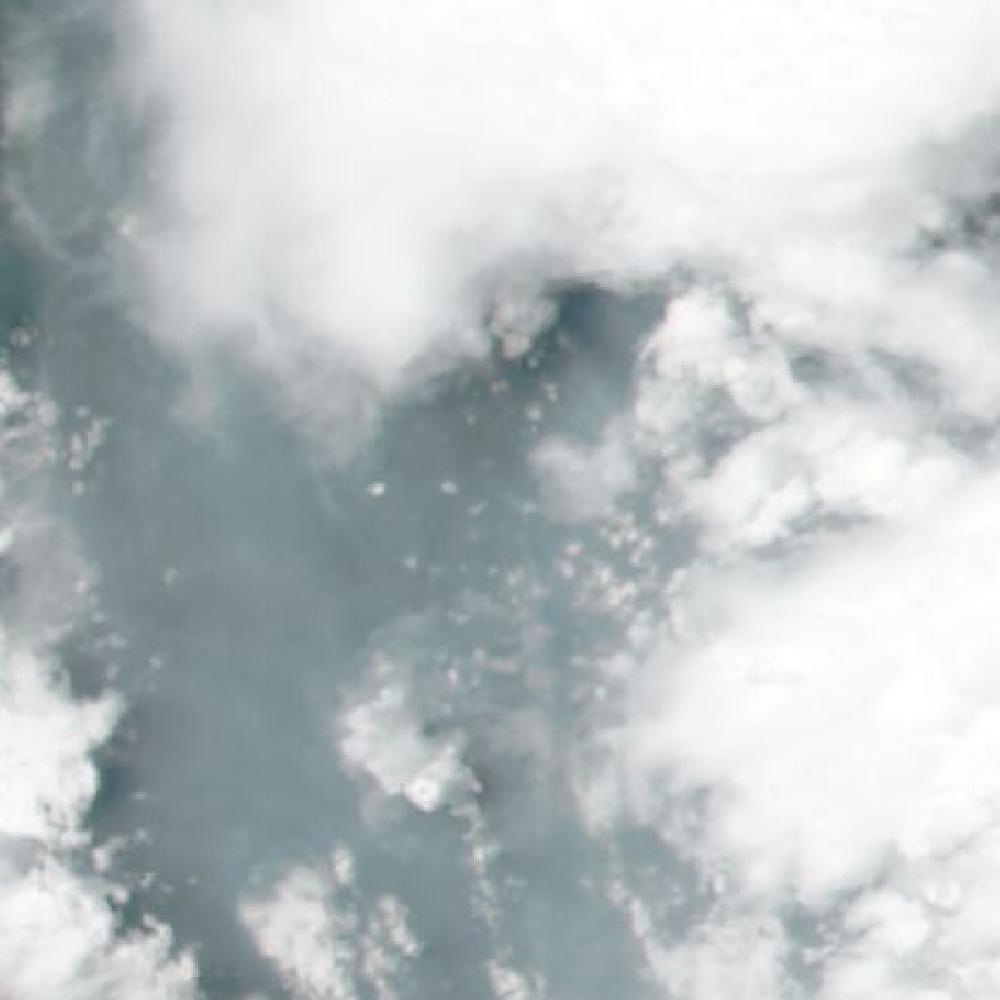
\includegraphics[width=\linewidth]{figuras/peru_selva_color.jpg}
\caption{Color verdadero: contraste visible y velo atmosférico.}
\end{subfigure}\hfill
\begin{subfigure}[t]{.485\textwidth}
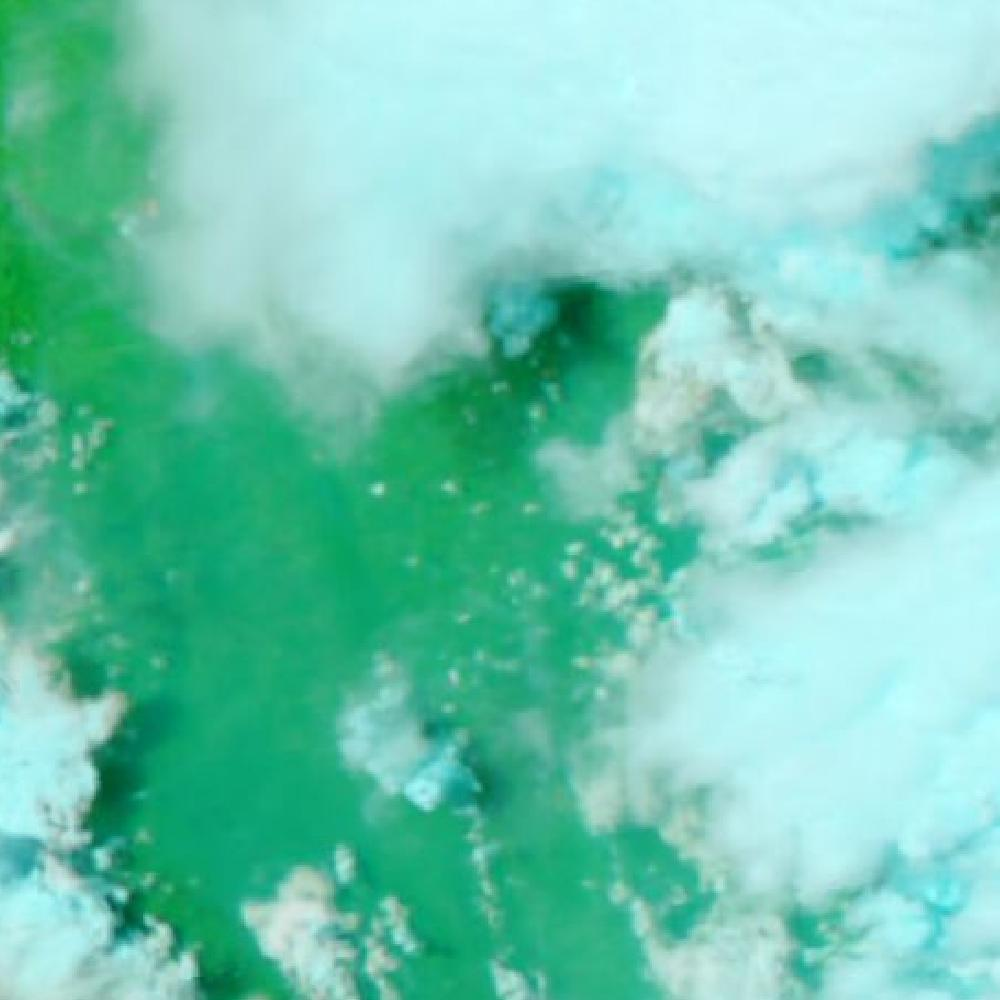
\includegraphics[width=\linewidth]{figuras/peru_selva_infrarrojo.jpg}
\caption{M11--I2--I1: otra respuesta espectral de la misma escena.}
\end{subfigure}
\caption{\textbf{Imágenes reales de Perú.} VIIRS/Suomi NPP, 15 de septiembre de 2024;
$10{,}5$--$9{,}5^\circ$ S, $75{,}5$--$74{,}5^\circ$ O, norte arriba. El recuadro mide
aproximadamente 111 km de norte a sur. Fuente: NASA GIBS/Worldview. Las manchas blancas
extensas siguen ocultando terreno; el cambio de colores no recupera esa información.}
\label{fig:peru-bandas}
\end{figure}

Observa primero la masa blanca de la parte superior y el borde derecho: no desaparece
en la composición infrarroja. Después compara la zona central: su contraste con el velo
gris cambia y la vegetación aparece verde en la composición M11--I2--I1. Ese verde es
una asignación de bandas a la pantalla, no una medición directa de salud vegetal.
Tampoco el velo permite diagnosticar su composición únicamente por este JPEG.

Esta pareja no se eligió para dibujar un contorno de incendio, sino para mostrar una
limitación: aun con bandas más informativas hay suelo que no vemos. El caso del
Camp Fire del capítulo~\ref{cap:problema} complementa la explicación al mostrar un
frente térmico visible y su transformación en puntos. En ambos casos, el pie de
imagen permite distinguir observación, representación e interpretación.

\section{El día y la noche}

De noche no hay Sol. Desaparece la componente reflejada a 4~\um, desaparece el brillo solar y
los suelos se han enfriado. La escena es más simple: todo lo que llega al sensor es emisión
térmica, y un píxel con exceso a 4~\um{} casi con seguridad contiene algo caliente de verdad.

Por eso los algoritmos usan umbrales \emph{distintos} de día y de noche, y por eso las
detecciones nocturnas tienen menos falsas alarmas. Los datos lo registran en la columna
\texttt{daynight}, con valores \texttt{D} y \texttt{N}.

Pero la noche tiene su propia trampa: el fuego también cambia. La mayoría de los incendios de
vegetación tiene un ciclo diario muy marcado, con máxima actividad a primera hora de la tarde,
cuando el aire está más caliente y seco y hay más viento, y mínima de madrugada. Muchas quemas
agrícolas se encienden por la mañana y están apagadas antes del anochecer. De noche se ve mejor,
pero hay menos que ver. El capítulo~\ref{cap:orbitas} retoma esta idea al hablar de la hora a la
que pasa cada satélite.

\begin{parareto}
La columna \texttt{daynight} permite separar detecciones diurnas y nocturnas. Para un calendario
de quemas agrícolas, las diurnas son las que capturan la actividad; las nocturnas señalan sobre
todo incendios que siguieron ardiendo sin control. Tratarlas por separado es una decisión de
diseño razonable y fácil de justificar.
\end{parareto}

\resumen

\begin{itemize}
  \item La atmósfera absorbe, dispersa y emite. Solo en las \textbf{ventanas atmosféricas} es
  suficientemente transparente; los canales de fuego están en la ventana de 3,5--4~\um{} y en
  la de 8--12,5~\um.
  \item El \textbf{humo} es casi transparente en el infrarrojo; las \textbf{nubes} espesas son
  opacas y ocultan el fuego sin dejar rastro en los datos.
  \item De día, el canal de 4~\um{} recibe emisión térmica \emph{y} luz solar reflejada en
  cantidades comparables; el de 11~\um{} solo emisión.
  \item Los principales impostores diurnos son el \textbf{brillo solar} sobre agua, los
  \textbf{suelos desnudos calientes} y los \textbf{bordes} de contraste.
  \item De noche la escena es más limpia y hay menos falsas alarmas, pero también menos fuego
  activo.
\end{itemize}

\ejercicios

\begin{enumerate}
  \item ¿Por qué no se coloca un canal de detección de fuego en 4,3~\um, donde las llamas emiten
  intensamente? Usa la figura~\ref{fig:ventanas}.
  \item Un píxel se observa a través de una atmósfera con $\tau = 0{,}85$ y la atmósfera aporta
  una radiancia propia de 0,05 unidades. Si la superficie emite 0,80 unidades, ¿qué radiancia
  llega al sensor según la ecuación~\eqref{eq:transferencia}? ¿Es mayor o menor que la que
  salió de la superficie?
  \item Explica por qué un incendio bajo una capa de humo espeso sí puede detectarse y uno bajo
  una nube espesa no.
  \item Un lago de la sierra aparece una tarde como una hilera de focos de baja confianza.
  Propón la explicación más probable y qué columna de los datos revisarías para apoyarla.
  \item Una región tiene su temporada de quemas en plena estación de lluvias, con el cielo
  cubierto la mitad de los días. ¿El conteo de focos subestima o sobrestima la actividad real?
  ¿Afecta esto por igual a MODIS y a VIIRS?
  \item Da dos razones por las que una detección nocturna es más fiable que una diurna y una
  razón por la que, pese a ello, un registro solo nocturno sería un mal calendario de quemas
  agrícolas.
\end{enumerate}


\part{Satélites y sensores}
\chapter{Órbitas: cuándo y cada cuánto pasa el satélite}\label{cap:orbitas}

\objetivos{
\begin{itemize}
  \item Calcular el periodo de un satélite a partir de su altura.
  \item Explicar qué es una órbita polar heliosíncrona y por qué el satélite cruza cada lugar
  siempre a la misma hora local.
  \item Decir a qué hora observa cada satélite de este libro y qué parte del ciclo diario del
  fuego capta.
  \item Explicar por qué MODIS deja huecos de cobertura cerca del ecuador y VIIRS no.
\end{itemize}}

\section{Por qué importa la órbita}

Un foco de calor es una observación instantánea. Qué fuegos entran en el registro depende, antes
que de cualquier algoritmo, de \emph{cuándo} mira el satélite y de \emph{cuántas veces} mira. Dos
sensores idénticos en órbitas distintas producirían registros distintos. Para comparar MODIS con
VIIRS hay que entender primero cómo se mueven sus plataformas.

\section{Movimiento orbital}

Un satélite en órbita está en caída libre permanente: avanza tan rápido en horizontal que, a
medida que cae, la superficie curva de la Tierra se aleja bajo él al mismo ritmo. Para una
órbita circular, la gravedad proporciona exactamente la fuerza centrípeta necesaria:
\begin{equation}
  \frac{G M m}{r^2} = \frac{m v^2}{r}
  \quad\Longrightarrow\quad
  v = \sqrt{\frac{GM}{r}},
\end{equation}
donde $r$ es la distancia al centro de la Tierra (radio terrestre más altura), y $GM =
\SI{3.986e5}{\kilo\metre\cubed\per\second\squared}$ es el parámetro gravitacional de la Tierra.
La masa del satélite se cancela: todos los objetos a la misma altura orbitan a la misma
velocidad.

El \termino{periodo} $P$, el tiempo de una vuelta completa, es la longitud de la circunferencia
dividida por la velocidad:
\begin{equation}\label{eq:periodo}
  P = \frac{2\pi r}{v} = 2\pi\sqrt{\frac{r^3}{GM}} .
\end{equation}
Esta es la tercera ley de Kepler para órbitas circulares.

\begin{ejemplo}{periodo de los satélites de MODIS y de VIIRS}
Terra y Aqua vuelan a 705~km de altura; Suomi NPP, NOAA-20 y NOAA-21, a unos 824~km. Con el
radio terrestre $R_\oplus = \SI{6378}{\kilo\metre}$, calcula su velocidad, su periodo y cuántas
órbitas dan al día.
\solucion Para MODIS, $r = 6378 + 705 = \SI{7083}{\kilo\metre}$.
\[
 v = \sqrt{\frac{\num{3.986e5}}{7083}} = \SI{7.50}{\kilo\metre\per\second},\qquad
 P = 2\pi\sqrt{\frac{7083^3}{\num{3.986e5}}} = \SI{5933}{\second} = \SI{98.9}{\minute}.
\]
En un día caben $1440/98{,}9 = 14{,}56$ órbitas. Para VIIRS, $r = \SI{7202}{\kilo\metre}$, y se
obtiene $v = \SI{7.44}{\kilo\metre\per\second}$, $P = \SI{101.4}{\minute}$ y 14,20 órbitas al
día. Ambos dan una vuelta al planeta en poco más de hora y media, a unos 27\,000~km/h.
\end{ejemplo}

\section{Órbita polar}

Si el satélite orbitara sobre el ecuador solo vería una franja ecuatorial. Para observar todo el
planeta se usa una \termino{órbita polar}: el satélite pasa cerca de los dos polos en cada
vuelta. La órbita mantiene su orientación en el espacio mientras la Tierra gira debajo, de modo
que en cada vuelta el satélite sobrevuela una franja distinta, desplazada hacia el oeste respecto
de la anterior (figura~\ref{fig:polar}).

\begin{figure}[ht]
\centering
\begin{tikzpicture}
  \begin{scope}
    \shade[ball color=cielo!45] (0,0) circle (2.3);
    \draw[ceniza!70] (-2.3,0) arc (180:360:2.3 and 0.55);
    \draw[ceniza!70,dashed] (2.3,0) arc (0:180:2.3 and 0.55);
    \draw[fuego,very thick] (0.35,2.9) arc (90:-90:0.75 and 2.9);
    \draw[fuego,very thick,dashed] (0.35,-2.9) arc (270:90:0.75 and 2.9);
    \fill[black] (1.02,1.3) circle (0.08);
    \draw[ceniza] (1.12,1.35)--(2.25,1.85);
    \node[anchor=west,font=\footnotesize,fill=white,inner sep=2pt] at (2.25,1.85) {satélite};
    \draw[->,thick] (2.75,0.5) arc (10:-35:1.2) node[midway,right,font=\footnotesize,align=left]{la Tierra\\ gira};
    \draw[->] (0,2.3)--(0,3.3) node[above,font=\footnotesize]{N};
    \node[font=\small\bfseries] at (0,-3.5) {(a) Órbita casi polar};
  \end{scope}
  \begin{scope}[shift={(8.2,0)}]
    \fill[cieloClaro] (-3.8,-2.2) rectangle (3.8,2.2);
    \draw[ceniza] (-3.8,-2.2) rectangle (3.8,2.2);
    \draw[ceniza,dashed] (-3.8,0)--(3.8,0) node[right,font=\footnotesize]{ecuador};
    \foreach \x/\n in {2.6/1,1.3/2,0/3,-1.3/4,-2.6/5}{
      \fill[fuego,opacity=0.22] (\x-0.75,-2.2)--(\x-0.15,-2.2)--(\x+0.55,2.2)--(\x-0.05,2.2)--cycle;
      \draw[fuego,thick,->] (\x-0.45,-2.2)--(\x+0.25,2.2);
      \node[font=\footnotesize] at (\x+0.25,2.45) {órbita \n};
    }
    \draw[<->] (1.2,-1.6)--(-0.1,-1.6) node[midway,below,font=\footnotesize]{$\approx$ 2750 km};
    \node[font=\small\bfseries] at (0,-3.5) {(b) Trazas sucesivas sobre el mapa};
  \end{scope}
\end{tikzpicture}
\caption{Órbita polar. (a) El plano de la órbita permanece casi fijo mientras la Tierra gira
debajo. (b) Vistas en un mapa, las pasadas sucesivas quedan desplazadas hacia el oeste; la franja
sombreada es la zona que el sensor alcanza a ver en cada pasada.}
\label{fig:polar}
\end{figure}

¿Cuánto se desplaza la traza entre una órbita y la siguiente? En el tiempo de una vuelta, la
Tierra gira una fracción $P/\SI{1440}{\minute}$ de su circunferencia. En el ecuador, cuya
longitud es de \SI{40075}{\kilo\metre}:
\begin{equation}\label{eq:separacion}
  d_{\text{ecuador}} = \SI{40075}{\kilo\metre}\times\frac{P}{\SI{1440}{\minute}} .
\end{equation}
Para MODIS resulta $40075 \times 98{,}9/1440 \approx \SI{2750}{\kilo\metre}$; para VIIRS, unos
\SI{2820}{\kilo\metre}. Recuerda estos dos números; volverán en la
sección~\ref{sec:huecos}.

\section{Órbita heliosíncrona: siempre a la misma hora}

Las órbitas de estos satélites no son exactamente polares. Tienen una inclinación de unos
98$^\circ$, es decir, pasan a unos 8$^\circ$ de los polos y giran en sentido ligeramente
contrario a la rotación terrestre. Esa pequeña desviación está elegida con un propósito.

La Tierra no es una esfera perfecta: está achatada, con un abultamiento en el ecuador. Ese
abultamiento tira del plano de la órbita y lo hace girar lentamente, como gira el eje de un
trompo inclinado. El fenómeno se llama \termino{precesión}. Escogiendo bien la altura y la
inclinación, se consigue que el plano orbital dé exactamente una vuelta al año,
$360^\circ/365{,}24 \approx 0{,}986^\circ$ por día, la misma velocidad angular con que la Tierra
gira alrededor del Sol.

\begin{definicion}{órbita heliosíncrona}
Una órbita heliosíncrona es aquella cuyo plano gira al mismo ritmo que la Tierra alrededor del
Sol, de modo que conserva una orientación fija respecto del Sol durante todo el año. Su
consecuencia práctica: el satélite cruza cada latitud siempre a la misma \textbf{hora solar
local}.
\end{definicion}

\begin{figure}[ht]
\centering
\begin{tikzpicture}[scale=0.95]
  \shade[inner color=yellow!80!white,outer color=brasa] (0,0) circle (0.5);
  \node[font=\footnotesize] at (0,-0.8) {Sol};
  \draw[ceniza!50,dashed] (0,0) circle (3.6);
  \foreach \a/\m in {0/marzo,90/junio,180/septiembre,270/diciembre}{
    \begin{scope}[shift={(\a:3.6)}]
      \shade[ball color=cielo!50] (0,0) circle (0.42);
      \draw[fuego,very thick,rotate=\a+90] (-0.85,0)--(0.85,0);
    \end{scope}
  }
  \node[font=\footnotesize,anchor=west] at (4.2,0) {marzo};
  \node[font=\footnotesize,anchor=south] at (0,4.25) {junio};
  \node[font=\footnotesize,anchor=east] at (-4.2,0) {septiembre};
  \node[font=\footnotesize,anchor=north] at (0,-4.25) {diciembre};
  \node[font=\footnotesize,align=left,fuego,anchor=west] at (5.8,1.0) {plano de la órbita\\ (visto de canto)};
  \node[font=\footnotesize,align=left,anchor=west] at (5.8,-0.6) {El plano mantiene el\\ mismo ángulo con la\\ dirección al Sol\\ todo el año.};
\end{tikzpicture}
\caption{Órbita heliosíncrona vista desde encima del polo norte. A lo largo del año el plano
orbital (línea roja) va girando para conservar su orientación respecto del Sol. Por eso el
satélite sobrevuela cada punto a la misma hora local en enero que en julio.}
\label{fig:helio}
\end{figure}

Para el fuego esto es fundamental. Si la hora de paso fuera variando a lo largo del año, el
sensor observaría unas veces el máximo de actividad de la tarde y otras la calma de la mañana, y
sería imposible separar los cambios reales de los cambios de horario. Con una órbita
heliosíncrona, la hora de observación es una constante del sistema.

\begin{definicion}{hora de cruce ecuatorial}
La hora de cruce ecuatorial es la hora solar local a la que el satélite atraviesa el ecuador.
Cada órbita tiene dos cruces, separados doce horas: el \emph{nodo ascendente}, cuando viaja de
sur a norte, y el \emph{nodo descendente}, de norte a sur.
\end{definicion}

\section{A qué hora mira cada satélite}

La tabla~\ref{tab:horas} reúne las horas nominales de cruce.

\begin{table}[ht]
\centering
\begin{tabular}{llccc}
\toprule
Satélite & Sensor & Altura & Cruce diurno & Cruce nocturno \\
\midrule
Terra & MODIS & 705 km & 10:30 & 22:30 \\
Aqua & MODIS & 705 km & 13:30 & 01:30 \\
Suomi NPP & VIIRS & 824 km & 13:30 & 01:30 \\
NOAA-20 & VIIRS & 824 km & 13:30 & 01:30 \\
NOAA-21 & VIIRS & 824 km & 13:30 & 01:30 \\
\bottomrule
\end{tabular}
\caption{Horas solares locales nominales de cruce del ecuador. Los tres satélites VIIRS
comparten la misma órbita, repartidos a lo largo de ella: NOAA-20 va media órbita (unos 50
minutos) separado de Suomi NPP, y NOAA-21 se sitúa entre ambos.}
\label{tab:horas}
\end{table}

Tres observaciones sobre la tabla, todas con consecuencias directas para la armonización.

\textbf{Aqua y los satélites VIIRS son compañeros de horario.} Todos cruzan a las 13:30. Aqua y
Suomi NPP observan los mismos fuegos casi a la misma hora, con diferencias que rara vez superan
unas decenas de minutos. Es la pareja natural para comparar los dos sensores.

\textbf{Terra no tiene sucesor.} Su pasada de las 10:30 capta el fuego de media mañana, y no
existe ningún VIIRS en ese horario. Cuando Terra se apague, esa ventana de observación
desaparecerá.

\textbf{Las horas son nominales.} En sus últimos años de vida, Terra y Aqua han dejado de hacer
las maniobras que mantenían su órbita, y sus horas de cruce se han ido desplazando: la de Terra
hacia más temprano y la de Aqua hacia más tarde. Para los años más recientes de MODIS la hora de
observación ya no es la de la tabla.

\begin{atencion}[La deriva orbital de MODIS]
Desde aproximadamente 2020--2022, Terra y Aqua derivan. Un cambio en la hora de paso altera qué
parte del ciclo diario del fuego se observa, y por tanto el número de focos, sin que el fuego
haya cambiado. Si tu calibración entre MODIS y VIIRS usa los últimos años del solape, parte de
la diferencia que midas se deberá a esta deriva. Es un buen motivo para calibrar con los años
centrales del solape (por ejemplo, 2012--2020) y decirlo expresamente.
\end{atencion}

\section{El ciclo diario del fuego}

¿Por qué tanta insistencia con la hora? Porque el fuego no arde igual a lo largo del día. La
humedad del aire es mínima y la temperatura y el viento son máximos a primera hora de la tarde;
el combustible está más seco y las llamas avanzan con más energía. Además, las quemas agrícolas
se encienden de día. El resultado es un \termino{ciclo diurno} muy marcado, con el máximo entre
las 13 y las 15 horas y el mínimo de madrugada (figura~\ref{fig:diurno}).

\begin{figure}[ht]
\centering
\begin{tikzpicture}
\begin{axis}[width=13.5cm,height=6.6cm,xmin=0,xmax=24,ymin=0,ymax=1.25,
  xlabel={Hora solar local},ylabel={Actividad de fuego (relativa)},
  xtick={0,3,6,9,12,15,18,21,24},ytick={0,0.5,1},yticklabels={0,{0,5},1},
  axis lines*=left,samples=200,domain=0:24]
\addplot[fill=fuego!25,draw=fuego,very thick] {0.04+exp(-((x-14)^2)/(2*2.6^2))} \closedcycle;
\foreach \h/\n/\c/\y in {10.5/Terra/modis/1.12,13.5/{Aqua y VIIRS}/viirs/1.2,22.5/Terra/modis/1.12}{
  \edef\temp{\noexpand\draw[\c,very thick,dashed] (axis cs:\h,0)--(axis cs:\h,\y-0.09);
             \noexpand\node[font=\noexpand\footnotesize,\c] at (axis cs:\h,\y-0.03) {\n};}
  \temp
}
\draw[viirs,very thick,dashed] (axis cs:1.5,0)--(axis cs:1.5,1.11);
\node[font=\footnotesize,viirs,anchor=west] at (axis cs:.25,1.17) {Aqua y VIIRS};
\end{axis}
\end{tikzpicture}
\caption{Forma típica del ciclo diario del fuego de vegetación (curva esquemática) y horas
nominales de paso. La pasada de las 13:30 cae cerca del máximo; la de las 10:30 encuentra los
fuegos todavía creciendo; las nocturnas ven solo lo que sobrevive a la noche.}
\label{fig:diurno}
\end{figure}

La forma exacta de la curva cambia con la región y con el tipo de fuego. Las quemas de residuos
agrícolas producen un pico estrecho, casi sin actividad nocturna; los grandes incendios
forestales tienen un ciclo más ancho y siguen ardiendo de noche.

\begin{ejemplo}{lo que ve cada pasada}
Supón que en una región la actividad sigue la curva de la figura~\ref{fig:diurno}, que
aproximaremos por una campana centrada en las 14:00 con desviación de 2,6 horas. ¿Qué fracción
del máximo observan la pasada de las 10:30 y la de las 13:30?
\solucion La campana vale $\exp[-(h-14)^2/(2\cdot 2{,}6^2)]$. A las 13:30, $h - 14 = -0{,}5$ y
el valor es $\exp(-0{,}018) = 0{,}98$. A las 10:30, $h-14 = -3{,}5$ y el valor es
$\exp(-0{,}906) = 0{,}40$. La pasada de la mañana encuentra menos de la mitad de la actividad
que la de la tarde. Un sensor que solo pasara a las 10:30 contaría, en esta región, alrededor
del 40\,{}\% de lo que cuenta uno que pasa a las 13:30, aunque ambos fueran idénticos.
\end{ejemplo}

\section{Franja de observación y huecos de cobertura}\label{sec:huecos}

El sensor no observa solo el punto que tiene debajo. Barre una franja perpendicular a su
trayectoria, la \termino{franja de barrido} o \emph{swath}, cuyo ancho depende de la altura y
del ángulo máximo con que mira hacia los lados. El punto situado exactamente bajo el satélite se
llama \termino{nadir}.

\begin{center}
\begin{tabular}{lcc}
\toprule
 & MODIS & VIIRS \\
\midrule
Ancho de la franja & 2330 km & 3040 km \\
Separación entre órbitas en el ecuador & 2750 km & 2820 km \\
\bottomrule
\end{tabular}
\end{center}

Compara las dos filas. La franja de MODIS es \emph{más estrecha} que la distancia entre trazas
consecutivas: en el ecuador, entre una pasada y la siguiente queda un hueco de unos 420~km que
ese día no se observa (figura~\ref{fig:huecos}). La franja de VIIRS es \emph{más ancha} que la
separación: las pasadas se solapan y no queda ningún hueco.

\begin{figure}[ht]
\centering
\begin{tikzpicture}[x=0.00175cm,y=1cm]
  \begin{scope}
    \node[font=\small\bfseries,modis] at (2750,2.1) {MODIS};
    \foreach \c in {0,2750,5500}{
      \fill[modis,opacity=0.3] (\c-1165,0) rectangle (\c+1165,1.4);
      \draw[modis,thick] (\c,0)--(\c,1.4);
    }
    \foreach \c in {1375,4125}{
      \fill[pattern=north east lines,pattern color=fuego] (\c-210,0) rectangle (\c+210,1.4);
    }
    \draw[<->] (0,-0.3)--(2750,-0.3) node[midway,below,font=\footnotesize]{2750 km};
    \draw[<->] (-1165,1.65)--(1165,1.65) node[midway,above,font=\footnotesize]{2330 km};
    \node[font=\footnotesize,fuego] at (4125,-0.35) {hueco};
  \end{scope}
  \begin{scope}[shift={(0,-4.2)}]
    \node[font=\small\bfseries,viirs] at (2820,2.1) {VIIRS};
    \foreach \c in {0,2820,5640}{
      \fill[viirs,opacity=0.25] (\c-1520,0) rectangle (\c+1520,1.4);
      \draw[viirs,thick] (\c,0)--(\c,1.4);
    }
    \draw[<->] (0,-0.3)--(2820,-0.3) node[midway,below,font=\footnotesize]{2820 km};
    \draw[<->] (-1520,1.65)--(1520,1.65) node[midway,above,font=\footnotesize]{3040 km};
    \node[font=\footnotesize] at (4230,0.7) {solape};
  \end{scope}
\end{tikzpicture}
\caption{Cobertura en el ecuador de tres órbitas consecutivas, a escala. MODIS deja franjas sin
observar (rayadas) entre pasadas; las franjas de VIIRS se solapan.}
\label{fig:huecos}
\end{figure}

A medida que aumenta la latitud las trazas convergen hacia los polos y los huecos de MODIS se
cierran; por encima de unos 30$^\circ$ ya no existen. Pero el Perú está entre 0$^\circ$ y
18$^\circ$ de latitud sur: de lleno en la zona de huecos.

\begin{intuicion}[Qué significa un hueco]
Los huecos no caen siempre en el mismo sitio; se desplazan de un día a otro. Para un lugar dado
cerca del ecuador, lo que ocurre es que algunos días, aproximadamente uno de cada seis o siete,
Aqua no lo observa de día. Ese día cualquier fuego en ese lugar es invisible para Aqua, pero no
para VIIRS. La figura~\ref{fig:worldview} del capítulo~\ref{cap:modisviirs} muestra un caso
real sobre el centro del Perú.
\end{intuicion}

\section{Número de observaciones por día}

Juntando todo, para un lugar de latitud baja como Junín, el número de oportunidades de
observación por día ha cambiado mucho a lo largo del registro:

\begin{center}
\begin{tabular}{lcl}
\toprule
Periodo & Pasadas diarias (día + noche) & Sensores \\
\midrule
2000--2002 & hasta 2 & Terra \\
2002--2011 & hasta 4 & Terra, Aqua \\
2012--2017 & hasta 4 MODIS + 2 VIIRS & + Suomi NPP \\
2018--2023 & hasta 4 MODIS + 4 VIIRS & + NOAA-20 \\
2024-- & hasta 4 MODIS + 6 VIIRS & + NOAA-21 \\
\bottomrule
\end{tabular}
\end{center}

<<Hasta>> porque los huecos de MODIS reducen el número real. La consecuencia es directa: si se
suman los focos de todos los satélites disponibles en cada época, el total crece simplemente
porque hay más ojos mirando.

\begin{parareto}
Antes de calibrar nada, \textbf{fija el conjunto de satélites} que entra en la serie. Una opción
limpia: usar solo Aqua para la era MODIS y solo Suomi NPP para la era VIIRS, que comparten la
hora de las 13:30. La columna \texttt{satellite} de los datos permite filtrar. Añadir NOAA-20 y
NOAA-21 mejora la detección reciente, pero rompe la comparabilidad con los años anteriores a
menos que se corrija expresamente.
\end{parareto}

\resumen

\begin{itemize}
  \item El periodo de una órbita circular depende solo de su altura:
  $P = 2\pi\sqrt{r^3/GM}$. MODIS orbita en unos 99 minutos y VIIRS en unos 101.
  \item Una órbita \textbf{polar} permite ver todo el planeta; una \textbf{heliosíncrona}
  garantiza que el satélite pase siempre a la misma hora solar local.
  \item \textbf{Terra} cruza a las 10:30/22:30; \textbf{Aqua} y los tres \textbf{VIIRS}, a las
  13:30/01:30. Aqua y Suomi NPP forman la pareja natural de comparación. Terra no tiene sucesor.
  \item El fuego tiene un \textbf{ciclo diurno} con máximo a primera hora de la tarde. La hora
  de paso determina qué fracción de la actividad se observa.
  \item Las órbitas de Terra y Aqua \textbf{derivan} en sus últimos años.
  \item La franja de MODIS (2330~km) deja \textbf{huecos} en latitudes bajas; la de VIIRS
  (3040~km) no.
  \item El número de satélites en vuelo ha cambiado; hay que fijar cuáles se usan.
\end{itemize}

\ejercicios

\begin{enumerate}
  \item Calcula el periodo de un satélite a 500~km de altura y el de uno a 1000~km. ¿Cuántas
  órbitas diarias da cada uno?
  \item Con la ecuación~\eqref{eq:separacion}, calcula la separación entre trazas consecutivas
  en el ecuador para un satélite con periodo de 95 minutos. ¿Qué ancho mínimo de franja necesita
  para no dejar huecos?
  \item La separación entre trazas a una latitud $\varphi$ es aproximadamente la del ecuador
  multiplicada por $\cos\varphi$. ¿A partir de qué latitud dejan de existir los huecos de
  MODIS? ¿Y a la latitud de Huancayo ($12^\circ$~S), cuánto mide el hueco?
  \item Con la campana del ejemplo de este capítulo, calcula qué fracción del máximo observa una
  pasada a las 15:00 y otra a las 09:00. Si Aqua deriva de las 13:30 hacia las 15:00, ¿sube o
  baja su conteo en esa región? ¿Y si Terra deriva de las 10:30 hacia las 09:00?
  \item Un compañero propone sumar los focos de Terra y Aqua para la era MODIS y los de Suomi
  NPP, NOAA-20 y NOAA-21 para la era VIIRS, <<para tener el máximo de datos>>. Escribe dos
  objeciones.
  \item ¿Por qué una órbita heliosíncrona necesita una inclinación mayor de 90$^\circ$ y no
  exactamente 90$^\circ$? Explícalo en un párrafo usando la idea de precesión.
\end{enumerate}

\chapter{Cómo se forma la imagen: píxeles y geometría de barrido}\label{cap:escaneo}

\objetivos{
\begin{itemize}
  \item Describir cómo un sensor de barrido transversal construye una imagen línea a línea.
  \item Explicar por qué los píxeles crecen hacia los bordes de la franja y calcular cuánto.
  \item Explicar el efecto pajarita y por qué produce detecciones repetidas del mismo fuego.
  \item Describir cómo VIIRS limita el crecimiento de sus píxeles y qué consecuencias tiene.
  \item Interpretar las columnas \texttt{scan} y \texttt{track} de los datos de focos.
\end{itemize}}

\section{Un espejo que gira}

MODIS y VIIRS no tienen una cámara con millones de sensores como la de un teléfono. Usan unos
pocos detectores y un espejo o telescopio giratorio. En cada giro, el instrumento recorre con la
mirada una línea del suelo perpendicular a la trayectoria del satélite, de un borde de la franja
al otro, tomando muestras a intervalos regulares. Mientras tanto el satélite avanza, de modo que
el giro siguiente recorre una línea un poco más adelante. La imagen se va tejiendo así, línea a
línea. Este diseño se llama \termino{barrido transversal} o \emph{whiskbroom}
(figura~\ref{fig:whisk}).

\begin{figure}[ht]
\centering
\begin{tikzpicture}[scale=0.92]
  \fill[bosque!18] (-6.2,-0.6)--(6.2,-0.6)--(7.6,1.6)--(-4.8,1.6)--cycle;
  \foreach \i in {0,1,2,3}{
    \fill[brasa!\the\numexpr25+15*\i\relax] (-5.9+0.2*\i,-0.4+0.4*\i)--(6.0+0.2*\i,-0.4+0.4*\i)--(6.2+0.2*\i,-0.05+0.4*\i)--(-5.7+0.2*\i,-0.05+0.4*\i)--cycle;
  }
  \begin{scope}[shift={(0.5,6)}]
    \fill[gray!45] (-0.45,-0.28) rectangle (0.45,0.28);
    \fill[cielo!70] (-1.7,-0.22) rectangle (-0.55,0.22); \fill[cielo!70] (0.55,-0.22) rectangle (1.7,0.22);
  \end{scope}
  \draw[->,very thick,ceniza] (2.6,6.0)--(3.9,6.6) node[right,font=\footnotesize,align=left]{avance del\\ satélite};
  \draw[fuego,thick] (0.5,5.7)--(-5.2,1.0); \draw[fuego,thick] (0.5,5.7)--(6.7,1.0);
  \draw[fuego,thick,dashed] (0.5,5.7)--(0.7,1.0);
  \draw[fuego,very thick,->] (-2.2,3.3) arc (215:325:3.3 and 1.1);
  \node[font=\footnotesize,fuego] at (1.6,2.25) {barrido};
  \node[font=\footnotesize] at (0.7,0.55) {nadir};
  \node[font=\footnotesize,align=center] at (-5.6,2.2) {borde de\\ la franja};
  \draw (0.5,4.6) arc (270:309:1.1); \node[font=\footnotesize] at (1.35,4.3) {$\theta$};
  \draw[<->] (-5.7,-0.9)--(6.2,-0.9) node[midway,below,font=\footnotesize]{ancho de la franja};
\end{tikzpicture}
\caption{Barrido transversal. El espejo recorre una línea de borde a borde; el avance del
satélite desplaza la línea siguiente. El ángulo $\theta$ entre la vertical y la dirección de
mirada es el \emph{ángulo de barrido}.}
\label{fig:whisk}
\end{figure}

Hay dos direcciones que conviene nombrar desde ya:

\begin{itemize}
  \item \textbf{a lo largo del barrido} (\emph{along-scan}): perpendicular al avance del
  satélite, la dirección en la que gira el espejo;
  \item \textbf{a lo largo de la traza} (\emph{along-track}): la dirección de avance.
\end{itemize}

\section{Qué es exactamente un píxel}

Cada detector ve, en cada instante, un cono muy estrecho de direcciones.

\begin{definicion}{campo de visión instantáneo (IFOV)}
El campo de visión instantáneo es el ángulo, medido desde el sensor, que abarca un detector en
un instante. Es una propiedad fija del instrumento. La porción de suelo que cae dentro de ese
ángulo es la \emph{huella} del píxel.
\end{definicion}

El ángulo es fijo; la huella no. En el nadir, a una altura $h$, un detector con IFOV $\alpha$
(en radianes) abarca en el suelo
\begin{equation}
  p_0 = h\,\alpha .
\end{equation}
Para MODIS, la huella de 1~km a 705~km de altura corresponde a
$\alpha = 1/705 = \SI{1.42e-3}{\radian}$, unos 0,08 grados.

\begin{atencion}[El píxel no es un cuadrado con bordes nítidos]
La respuesta del detector no es uniforme dentro de la huella ni cae a cero justo en su borde.
Además, el espejo se mueve mientras se toma la muestra. En MODIS esto hace que la huella efectiva
a lo largo del barrido sea más ancha que el espaciado entre muestras: las huellas de píxeles
vecinos se \textbf{solapan} en parte. Un fuego pequeño e intenso situado cerca del límite entre
dos píxeles puede elevar la señal de ambos y ser detectado dos veces en la misma línea.
\end{atencion}

\section{Los píxeles crecen hacia los bordes}

Cuando el espejo apunta hacia un lado, el mismo cono angular alcanza el suelo más lejos y,
además, en oblicuo. Ambas cosas agrandan la huella (figura~\ref{fig:crecimiento}).

\begin{figure}[ht]
\centering
\begin{tikzpicture}[scale=1.0]
  \draw[bosque,very thick] (-1,0)--(11.5,0);
  \fill (1,5) circle (0.09) node[above,font=\footnotesize]{sensor};
  \draw[dashed,ceniza] (1,5)--(1,0);
  \fill[fuego,opacity=0.3] (1,5)--(0.72,0)--(1.28,0)--cycle;
  \draw[fuego] (1,5)--(0.72,0) (1,5)--(1.28,0);
  \fill[fuego,opacity=0.3] (1,5)--(5.45,0)--(6.6,0)--cycle;
  \draw[fuego] (1,5)--(5.45,0) (1,5)--(6.6,0);
  \fill[fuego,opacity=0.3] (1,5)--(8.4,0)--(11.2,0)--cycle;
  \draw[fuego] (1,5)--(8.4,0) (1,5)--(11.2,0);
  \draw[very thick,black] (0.72,-0.12)--(1.28,-0.12);
  \draw[very thick,black] (5.45,-0.12)--(6.6,-0.12);
  \draw[very thick,black] (8.4,-0.12)--(11.2,-0.12);
  \node[below,font=\footnotesize] at (1,-0.2) {nadir};
  \node[below,font=\footnotesize] at (6,-0.2) {$\theta$ medio};
  \node[below,font=\footnotesize] at (9.8,-0.2) {$\theta$ grande};
  \draw (1,3.9) arc (270:316:1.1); \node[font=\footnotesize] at (1.65,3.75) {$\theta$};
  \draw[<->] (0.6,5)--(0.6,0) node[midway,left,font=\footnotesize]{$h$};
\end{tikzpicture}
\caption{El mismo ángulo de visión cubre cada vez más suelo conforme la mirada se inclina (vista
de perfil, Tierra plana para simplificar).}
\label{fig:crecimiento}
\end{figure}

Con una Tierra plana, la geometría es elemental. La distancia del sensor al suelo en la
dirección $\theta$ es $h/\cos\theta$, así que la huella crece en ese factor en la dirección de
avance. A lo largo del barrido hay un segundo factor $1/\cos\theta$, porque el cono corta el
suelo en oblicuo:
\begin{equation}\label{eq:plano}
  p_{\text{traza}} \approx \frac{p_0}{\cos\theta},
  \qquad
  p_{\text{barrido}} \approx \frac{p_0}{\cos^2\theta}
  \qquad\text{(Tierra plana).}
\end{equation}

La Tierra, sin embargo, es curva, y cerca de los bordes de una franja de más de 2000~km la
curvatura importa mucho: el suelo <<se aleja>> del sensor más de lo que predice el modelo plano
y la mirada llega aún más rasante. El cálculo exacto usa el triángulo formado por el centro de la
Tierra, el satélite y el punto observado (figura~\ref{fig:curva}). Si $R$ es el radio terrestre,
el ángulo $\beta$ con que la línea de mirada llega al suelo, medido desde la vertical local, se
obtiene con el teorema del seno:
\begin{equation}\label{eq:cenit}
  \sin\beta = \frac{R+h}{R}\,\sin\theta ,
\end{equation}
y las dimensiones de la huella son
\begin{equation}\label{eq:curvo}
  p_{\text{traza}} = p_0\,\frac{d}{h},
  \qquad
  p_{\text{barrido}} = p_0\,\frac{d}{h}\,\frac{1}{\cos\beta},
\end{equation}
donde $d$ es la distancia real del sensor al punto observado.

\begin{figure}[ht]
\centering
% O es el centro común de ambos radios; h y los ángulos se dibujan aparte.
\begin{tikzpicture}[scale=.95,font=\footnotesize]
  \coordinate (O) at (0,0);
  \coordinate (S) at (0,6.3);
  \coordinate (N) at (0,5);
  \coordinate (P) at (67:5);
  \draw[bosque,very thick] (50:5) arc (50:130:5);
  \draw[ceniza,dashed] (O)--(N) node[midway,left] {$R$};
  \draw[ceniza,dashed] (N)--(S);
  \draw[ceniza,dashed] (O)--(P) node[pos=.45,right] {$R$};
  \fill (O) circle (.06) node[below=3pt] {centro de la Tierra};
  \fill (S) circle (.08) node[above=3pt] {satélite};
  \fill (P) circle (.07);
  \node[anchor=west] at ($(P)+(.2,-.15)$) {punto observado};
  \draw[fuego,thick] (S)--(P) node[midway,above right] {$d$};
  \draw[ceniza,dashed] (P)--($(P)+(67:1.5)$);
  \node[anchor=west] at ($(P)+(67:1.65)$) {vertical local};
  \draw[<->] (-.5,5)--(-.5,6.3) node[midway,left] {$h$};
  \draw (0,5.65) arc[start angle=270,end angle=319,radius=.65];
  \node at (.33,5.22) {$\theta$};
  \draw ($(P)+(67:.55)$) arc[start angle=67,end angle=139,radius=.55];
  \node at ($(P)+(103:.85)$) {$\beta$};
\end{tikzpicture}

\caption{Con la Tierra curva, la mirada llega al suelo con un ángulo $\beta$ respecto de la
vertical local que es mayor que el ángulo de barrido $\theta$. Los dos radios parten
del mismo centro terrestre. Esquema geométrico, no a escala.}
\label{fig:curva}
\end{figure}

\begin{ejemplo}{el píxel de MODIS en el borde de la franja}
MODIS barre hasta $\theta = 55^\circ$. Calcula el tamaño de su píxel de 1~km en el borde, con el
modelo plano y con el modelo curvo ($R = \SI{6371}{\kilo\metre}$, $h = \SI{705}{\kilo\metre}$).
\solucion \emph{Modelo plano.} $\cos 55^\circ = 0{,}574$. Entonces
$p_{\text{traza}} = 1/0{,}574 = \SI{1.74}{\kilo\metre}$ y
$p_{\text{barrido}} = 1/0{,}574^2 = \SI{3.04}{\kilo\metre}$.

\emph{Modelo curvo.} De~\eqref{eq:cenit}: $\sin\beta = (7076/6371)\times\sin 55^\circ =
0{,}910$, luego $\beta = 65{,}5^\circ$. El ángulo en el centro de la Tierra es $\beta - \theta =
10{,}5^\circ$, y por el teorema del seno $d = R\,\sin(10{,}5^\circ)/\sin(55^\circ) =
\SI{1414}{\kilo\metre}$. Con~\eqref{eq:curvo}:
\[
 p_{\text{traza}} = 1\times\frac{1414}{705} = \SI{2.01}{\kilo\metre},
 \qquad
 p_{\text{barrido}} = \frac{2{,}01}{\cos 65{,}5^\circ} = \SI{4.83}{\kilo\metre}.
\]
El píxel de <<1~km>> mide en el borde unos $2{,}0 \times 4{,}8$~km: casi diez veces más área que
en el nadir. El modelo plano se queda muy corto.
\end{ejemplo}

Este crecimiento tiene una consecuencia directa sobre la detección. Como se verá en el
capítulo~\ref{cap:deteccion}, un fuego se detecta cuando eleva lo suficiente la señal de
\emph{su} píxel. Si el píxel tiene diez veces más área, el mismo fuego queda diez veces más
diluido. \textbf{MODIS es mucho menos sensible en los bordes de su franja que en el centro.}

\section{El efecto pajarita}

MODIS no tiene un solo detector por banda sino una fila de diez, alineados en la dirección de
avance. En cada giro del espejo se registran diez líneas a la vez, que en el nadir cubren una
banda de 10~km de ancho en la dirección de avance; el satélite avanza justo esos 10~km entre un
giro y el siguiente, y las bandas encajan sin solaparse.

Pero hacia los bordes cada píxel crece también en la dirección de avance: en el extremo, las
diez líneas cubren unos 20~km en lugar de 10. El satélite sigue avanzando 10~km por giro, así
que cada barrido \textbf{pisa} la mitad del anterior y la mitad del siguiente. Visto en un mapa,
cada barrido tiene forma de corbata de lazo: estrecho en el centro y ancho en los extremos. De
ahí el nombre \termino{efecto pajarita} (\emph{bow-tie}), que muestra la
figura~\ref{fig:bowtie}.

\begin{figure}[ht]
\centering
\begin{tikzpicture}[x=0.85cm,y=1cm]
  \foreach \k/\c in {0/modis,1/fuego,2/bosque}{
    \fill[\c,opacity=0.28] (-6,\k*1.0-1.0)--(0,\k*1.0-0.5)--(6,\k*1.0-1.0)--(6,\k*1.0+1.0)--(0,\k*1.0+0.5)--(-6,\k*1.0+1.0)--cycle;
    \draw[\c,thick] (-6,\k*1.0-1.0)--(0,\k*1.0-0.5)--(6,\k*1.0-1.0)--(6,\k*1.0+1.0)--(0,\k*1.0+0.5)--(-6,\k*1.0+1.0)--cycle;
  }
  \node[font=\footnotesize,modis] at (-1.3,0) {barrido 1};
  \node[font=\footnotesize,fuego] at (0,1) {barrido 2};
  \node[font=\footnotesize,bosque] at (0,2) {barrido 3};
  \shade[inner color=yellow,outer color=fuego] (5.3,0.75) circle (0.13);
  \draw[<-,thick] (5.45,0.75)--(6.6,0.75) node[right,font=\footnotesize,align=left]{este fuego cae\\ en dos barridos};
  \draw[->,thick,ceniza] (-6.9,-0.8)--(-6.9,2.8) node[above,font=\footnotesize]{avance};
  \draw[<->] (-6,-1.5)--(6,-1.5) node[midway,below,font=\footnotesize]{franja de barrido (nadir en el centro)};
  \draw[<->] (0,-0.5)--(0,0.5);
  \node[font=\footnotesize,modis,fill=white,inner sep=1.5pt] at (1.3,-.25) {10 km};
  \draw[<->] (-6.25,-1)--(-6.25,1); \node[left,font=\footnotesize] at (-6.3,0) {20 km};
\end{tikzpicture}
\caption{El efecto pajarita en MODIS. Cada barrido registra una banda de 10~km de ancho en el
nadir que se ensancha hasta unos 20~km en los bordes. Barridos consecutivos se solapan lejos del
nadir, y un fuego situado allí queda registrado en dos de ellos.}
\label{fig:bowtie}
\end{figure}

\begin{atencion}[Focos duplicados dentro de una misma pasada]
Lejos del nadir, un mismo fuego puede aparecer como dos o más focos de MODIS con coordenadas
ligeramente distintas y exactamente la misma hora. No son dos fuegos. Si se cuentan <<puntos>>
sin más, los fuegos observados de lado pesan más que los observados desde arriba.
\end{atencion}

\section{La solución de VIIRS}

VIIRS se diseñó para corregir estos dos defectos. Usa dos ideas.

\subsection{Agregación de muestras}

Los detectores de VIIRS son, a lo largo del barrido, tres veces más finos de lo que el producto
final necesita. Cerca del nadir, el instrumento \emph{promedia tres muestras consecutivas} para
formar un píxel de 375~m. Más lejos, cuando cada muestra ya ha crecido, promedia solo dos. En la
parte exterior de la franja usa cada muestra tal cual. Hay así tres zonas de agregación:

\begin{center}
\begin{tabular}{lcc}
\toprule
Zona & Ángulo de barrido & Muestras promediadas \\
\midrule
Central & $0^\circ$ a $31{,}7^\circ$ & 3 \\
Intermedia & $31{,}7^\circ$ a $44{,}9^\circ$ & 2 \\
Exterior & $44{,}9^\circ$ a $56{,}3^\circ$ & 1 \\
\bottomrule
\end{tabular}
\end{center}

Cada vez que el píxel está a punto de crecer demasiado, se reduce el número de muestras y el
tamaño <<se reinicia>>. El resultado es la curva en dientes de sierra de la
figura~\ref{fig:tamano}: el píxel de 375~m de VIIRS no pasa de unos 800~m en el borde de la
franja, mientras que el de MODIS llega casi a 5~km.

\begin{figure}[ht]
\centering
\begin{tikzpicture}
\begin{axis}[width=13.5cm,height=7.4cm,xmin=0,xmax=1550,ymin=0,ymax=5.2,
  xlabel={Distancia al nadir sobre el suelo (km)},
  ylabel={Tamaño del píxel a lo largo del barrido (km)},
  ytick={0,1,2,3,4,5},
  legend style={at={(0.5,-0.2)},anchor=north,font=\small,draw=none,legend columns=2,/tikz/every even column/.append style={column sep=8pt}},
  grid=major,grid style={ceniza!15}]
\addplot[modis,very thick] table[x=dist,y=scan]{figuras/pixel_modis.dat};
\addplot[viirs,very thick] table[x=dist,y=scan]{figuras/pixel_viirs.dat};
\addplot[modis,thick,dashed] table[x=dist,y=track]{figuras/pixel_modis.dat};
\addplot[viirs,thick,dashed] table[x=dist,y=track]{figuras/pixel_viirs.dat};
\legend{MODIS a lo largo del barrido,VIIRS 375 m a lo largo del barrido,MODIS a lo largo de la traza,VIIRS 375 m a lo largo de la traza}
\draw[ceniza,dashed] (axis cs:523,0)--(axis cs:523,1.6);
\draw[ceniza,dashed] (axis cs:883,0)--(axis cs:883,1.6);
\node[font=\footnotesize,ceniza] at (axis cs:260,1.85) {3 muestras};
\node[font=\footnotesize,ceniza] at (axis cs:703,1.85) {2};
\node[font=\footnotesize,ceniza] at (axis cs:1200,1.85) {1 muestra};
\draw[->,ceniza] (axis cs:1300,4.3)--(axis cs:1175,4.75);
\node[font=\footnotesize,anchor=east] at (axis cs:1310,4.2) {borde de la franja de MODIS};
\end{axis}
\end{tikzpicture}
\caption{Tamaño del píxel según la distancia al nadir, calculado con las
ecuaciones~\eqref{eq:cenit} y~\eqref{eq:curvo}. El píxel de MODIS se multiplica casi por cinco
a lo largo del barrido; el de VIIRS, gracias a la agregación en tres zonas, se mantiene por
debajo de 0,8~km en toda la franja.}
\label{fig:tamano}
\end{figure}

\subsection{Eliminación del solape}

VIIRS también sufre el efecto pajarita, pero lo resuelve a bordo: en las zonas intermedia y
exterior, el propio instrumento descarta las líneas de cada barrido que quedarían duplicadas en
el barrido vecino. A esto se le llama \termino{eliminación de pajarita} (\emph{bow-tie
deletion}). Los datos de VIIRS llegan así casi sin repeticiones entre barridos de una misma
pasada.

\section{Las columnas \texttt{scan} y \texttt{track}}

Los datos de focos incluyen para cada detección el tamaño real del píxel en el que se hizo. La
columna \texttt{scan} es su dimensión a lo largo del barrido y \texttt{track} a lo largo de la
traza, ambas en kilómetros. En MODIS, \texttt{scan} va de 1,0 a 4,8 y \texttt{track} de 1,0 a
2,0. En VIIRS ambos se mantienen entre 0,3 y 0,8 aproximadamente.

Estas dos columnas son la manera más directa de saber \emph{desde dónde} se observó cada foco:
un valor de \texttt{scan} cercano a 1 en MODIS indica una observación casi vertical; un valor de
4 indica el borde de la franja.

\begin{ejemplo}{interpretar \texttt{scan} y \texttt{track}}
Un foco de MODIS tiene \texttt{scan} = 2,9 y \texttt{track} = 1,6. ¿Qué área cubre su píxel y a
qué distancia aproximada del nadir se observó? Un fuego de 1000~m$^2$, ¿qué fracción del píxel
ocupa aquí y qué fracción ocuparía en el nadir?
\solucion El área es aproximadamente $2{,}9 \times 1{,}6 = \SI{4.6}{\kilo\metre\squared}$. En
la figura~\ref{fig:tamano}, un tamaño de 2,9~km a lo largo del barrido corresponde a unos
860--880~km del nadir. El fuego ocupa $1000/\num{4.6e6} = \num{2.2e-4}$ del píxel, frente a
$1000/\num{1.0e6} = \num{1.0e-3}$ en el nadir: está casi cinco veces más diluido.
\end{ejemplo}

\begin{parareto}
Dos usos prácticos de estas columnas. Primero, como \textbf{filtro de calidad}: quedarse solo
con las detecciones de MODIS con \texttt{scan} menor que cierto valor (por ejemplo 2) elimina
la parte de la franja donde MODIS es poco sensible y donde aparecen duplicados. Segundo, como
\textbf{diagnóstico}: si la razón entre los conteos de VIIRS y de MODIS es mucho mayor para
detecciones de MODIS con \texttt{scan} alto, estás viendo directamente el efecto de este
capítulo. Cualquier filtro reduce el número de datos, así que hay que aplicarlo igual en todo el
periodo y documentarlo.
\end{parareto}

\section{Resolución espacial y tamaño mínimo detectable}

Queda una idea por fijar. Se suele decir que MODIS tiene <<1~km de resolución>> y VIIRS <<375
m>>. Eso describe el tamaño del píxel, no el tamaño del fuego más pequeño que pueden detectar.
Ambos detectan fuegos \emph{mucho} menores que su píxel, porque el fuego es tan brillante a
4~\um{} que una fracción diminuta del píxel basta para alterar su señal. Bajo buenas
condiciones, MODIS detecta de forma habitual fuegos de unos 1000~m$^2$ (una milésima de su
píxel) y, en condiciones muy favorables, de unos 100~m$^2$. VIIRS, con píxeles siete veces
menores en área, detecta fuegos proporcionalmente más pequeños. El capítulo~\ref{cap:deteccion}
explica el porqué con números.

\resumen

\begin{itemize}
  \item MODIS y VIIRS forman la imagen por \textbf{barrido transversal}: un espejo recorre
  líneas perpendiculares al avance.
  \item El \textbf{IFOV} es un ángulo fijo; la huella en el suelo crece con el ángulo de
  barrido. Con la Tierra curva el crecimiento es mucho mayor que con el modelo plano.
  \item El píxel de MODIS pasa de $1\times1$~km en el nadir a unos $2{,}0\times4{,}8$~km en el
  borde: diez veces más área y mucha menos sensibilidad.
  \item El \textbf{efecto pajarita} hace que barridos consecutivos se solapen lejos del nadir y
  produce focos duplicados en MODIS.
  \item VIIRS limita el crecimiento con \textbf{agregación en tres zonas} (su píxel de 375~m no
  supera 0,8~km) y elimina a bordo las líneas solapadas.
  \item Las columnas \texttt{scan} y \texttt{track} dan el tamaño real del píxel de cada foco.
\end{itemize}

\ejercicios

\begin{enumerate}
  \item Calcula el IFOV, en radianes y en grados, de la banda de 375~m de VIIRS a 824~km de
  altura. ¿Es mayor o menor que el de MODIS?
  \item Con el modelo plano, ¿a qué ángulo de barrido se duplica el tamaño del píxel a lo largo
  del barrido? ¿Y a lo largo de la traza?
  \item Repite el ejemplo del borde de la franja para $\theta = 40^\circ$ con el modelo curvo.
  ¿Cuántas veces mayor que en el nadir es el área del píxel?
  \item En la figura~\ref{fig:tamano}, estima el cociente entre el área del píxel de MODIS y el
  de VIIRS en el nadir y a 1100~km del nadir. ¿Dónde es mayor la ventaja de VIIRS?
  \item Explica por qué el efecto pajarita produce duplicados en los bordes de la franja pero no
  en el centro.
  \item Tienes un archivo de focos de MODIS de una región. Describe un procedimiento, usando
  solo las columnas de fecha, hora, coordenadas, \texttt{scan} y \texttt{track}, para identificar
  parejas de focos que probablemente sean el mismo fuego visto en dos barridos.
  \item Un colega dice: <<MODIS no puede ver fuegos menores de un kilómetro>>. Corrígelo en dos
  frases.
\end{enumerate}

\chapter{MODIS y VIIRS frente a frente}\label{cap:modisviirs}

\objetivos{
\begin{itemize}
  \item Describir cada instrumento: plataformas, bandas usadas para el fuego y resolución.
  \item Explicar qué es la saturación de un detector y cómo afecta a cada sensor.
  \item Enumerar todas las diferencias entre MODIS y VIIRS que influyen en el número de focos.
  \item Leer una imagen real en la que ambos sensores observan la misma región el mismo día.
\end{itemize}}

\section{Dos generaciones}

Los capítulos anteriores han ido presentando piezas sueltas de los dos instrumentos. Este las
reúne. Leerlo con atención vale la pena: la lista de diferencias de la
sección~\ref{sec:diferencias} es, en la práctica, la lista de cosas que la armonización tiene
que corregir.

\section{MODIS}

MODIS es un radiómetro de 36 bandas espectrales, desde el visible hasta el infrarrojo térmico,
diseñado en los años noventa como instrumento de propósito general del Sistema de Observación de
la Tierra de la NASA. Se construyeron dos unidades casi idénticas:

\begin{itemize}
  \item \textbf{Terra}, lanzado en diciembre de 1999, en órbita de mañana (10:30);
  \item \textbf{Aqua}, lanzado en mayo de 2002, en órbita de tarde (13:30).
\end{itemize}

Las 36 bandas tienen tres resoluciones distintas en el nadir: 250~m (2 bandas), 500~m (5
bandas) y 1~km (29 bandas). Todas las bandas térmicas son de 1~km, y por eso el producto de
fuego tiene esa resolución. Las que usa el algoritmo de fuego son las de la
tabla~\ref{tab:bandas-modis}.

\begin{table}[ht]
\centering
\begin{tabular}{clcl}
\toprule
Banda & Longitud de onda & Saturación & Papel en la detección \\
\midrule
21 & 3,96 \um & $\approx 500$ K & canal de fuego, rango alto \\
22 & 3,96 \um & $\approx 331$ K & canal de fuego, rango bajo y menos ruido \\
31 & 11,0 \um & $\approx 400$ K (Terra) & temperatura del fondo, nubes \\
   &  & $\approx 340$ K (Aqua) & \\
32 & 12,0 \um & & máscara de nubes \\
1, 2 & 0,65 y 0,86 \um & & reflectancia: nubes, agua, brillo solar \\
7 & 2,1 \um & & rechazo de brillo solar y costas \\
\bottomrule
\end{tabular}
\caption{Bandas de MODIS que intervienen en la detección de fuego.}
\label{tab:bandas-modis}
\end{table}

Llama la atención que haya \emph{dos} bandas en la misma longitud de onda. La razón es la
saturación.

\section{Saturación}

Un detector convierte radiancia en una señal eléctrica, y la electrónica solo puede representar
un intervalo limitado de valores. Si la radiancia supera el máximo, el detector entrega su valor
tope y ya no dice cuánto más había.

\begin{definicion}{saturación}
Un detector se satura cuando la radiancia que recibe supera el máximo que puede medir. La
\emph{temperatura de saturación} es la temperatura de brillo correspondiente a ese máximo. Por
encima de ella todas las mediciones valen lo mismo.
\end{definicion}

Hay aquí un compromiso inevitable. Un detector pensado para medir con precisión temperaturas de
la superficie (entre 250 y 330~K) se satura enseguida con un fuego. Uno pensado para no saturarse
con un fuego mide el fondo con poco detalle y más ruido. MODIS lo resuelve con las dos bandas de
4~\um: la \textbf{22} es precisa pero se satura hacia 331~K; la \textbf{21} es ruidosa pero
aguanta hasta unos 500~K. El algoritmo usa la banda 22 siempre que puede y cambia a la 21 cuando
la 22 se satura. En ambos casos el resultado se llama simplemente $T_4$.

\begin{figure}[ht]
\centering
\begin{tikzpicture}
\begin{axis}[width=12.5cm,height=6.4cm,xmin=280,xmax=560,ymin=280,ymax=560,
  xlabel={Temperatura de brillo real del píxel (K)},
  ylabel={Temperatura de brillo medida (K)},
  legend style={at={(0.03,0.96)},anchor=north west,font=\small,draw=ceniza!40},
  grid=major,grid style={ceniza!15}]
\addplot[ceniza,dashed,domain=280:560] {x};
\addplot[modis,very thick] coordinates {(280,280)(331,331)(560,331)};
\addplot[modis!55,very thick,dashdotted] coordinates {(280,280)(500,500)(560,500)};
\addplot[viirs,very thick] coordinates {(280,280)(367,367)(560,367)};
\legend{medición ideal,MODIS banda 22,MODIS banda 21,VIIRS banda I4}
\end{axis}
\end{tikzpicture}
\caption{Respuesta de los canales de 4~\um{} (esquema). Cada detector sigue a la temperatura
real hasta su punto de saturación y a partir de ahí se queda plano.}
\label{fig:saturacion}
\end{figure}

\section{VIIRS}

VIIRS es el instrumento que sucede a MODIS (y al más antiguo AVHRR) dentro del sistema de
satélites meteorológicos polares de Estados Unidos. Vuela en:

\begin{itemize}
  \item \textbf{Suomi NPP}, lanzado en octubre de 2011;
  \item \textbf{NOAA-20}, lanzado en noviembre de 2017;
  \item \textbf{NOAA-21}, lanzado en noviembre de 2022.
\end{itemize}

Los tres comparten la órbita de las 13:30. VIIRS tiene 22 bandas de dos tipos: las bandas
\textbf{I} (de \emph{imagery}), con 375~m de resolución en el nadir, y las bandas \textbf{M}
(de \emph{moderate}), con 750~m. Existen dos productos de fuego, uno por cada resolución; el que
distribuye FIRMS como producto principal, y el que nos ocupa, es el de \textbf{375~m}.

\begin{table}[ht]
\centering
\begin{tabular}{clcl}
\toprule
Banda & Longitud de onda & Saturación & Papel en la detección \\
\midrule
I4 & 3,74 \um & 367 K & canal de fuego \\
I5 & 11,45 \um & $\approx 380$ K & temperatura del fondo, nubes \\
I1, I2, I3 & 0,64; 0,86; 1,61 \um & & nubes, agua, brillo solar \\
M13 & 4,05 \um{} (750 m) & $\approx 634$ K & potencia radiativa del fuego \\
\bottomrule
\end{tabular}
\caption{Bandas de VIIRS que intervienen en el producto de fuego de 375~m.}
\label{tab:bandas-viirs}
\end{table}

Dos detalles de la tabla tendrán consecuencias más adelante. El canal de fuego I4 está en
3,74~\um, no en 3,96: algo más lejos de la absorción del CO$_2$ y algo más sensible a la luz
solar reflejada. Y se satura a 367~K, una temperatura que un fuego mediano alcanza con facilidad
en un píxel tan pequeño. Por eso la \emph{potencia} del fuego no se calcula con I4 sino con la
banda M13, de 750~m, que tiene un rango mucho mayor (capítulo~\ref{cap:frp}).

\section{La comparación completa}\label{sec:diferencias}

\begin{table}[ht]
\centering
\renewcommand{\arraystretch}{1.25}
\begin{tabularx}{\textwidth}{>{\raggedright\arraybackslash}p{4.2cm}>{\raggedright\arraybackslash}X>{\raggedright\arraybackslash}X}
\toprule
 & \textbf{MODIS} & \textbf{VIIRS (375 m)} \\
\midrule
Satélites & Terra, Aqua & Suomi NPP, NOAA-20, NOAA-21 \\
Datos de focos desde & noviembre de 2000 & enero de 2012 \\
Altura de la órbita & 705 km & 824 km \\
Hora de cruce & 10:30 y 13:30 & 13:30 \\
Ancho de la franja & 2330 km (huecos en el ecuador) & 3040 km (sin huecos) \\
Píxel en el nadir & 1 km & 375 m \\
Píxel en el borde & $\approx 2{,}0 \times 4{,}8$ km & $\approx 0{,}8 \times 0{,}8$ km \\
Área del píxel (nadir) & 1 km$^2$ & 0,14 km$^2$ \\
Canal de fuego & 3,96 \um{} (bandas 21 y 22) & 3,74 \um{} (I4) \\
Canal de fondo & 11,0 \um{} (banda 31) & 11,45 \um{} (I5) \\
Saturación a 4 \um & $\approx 500$ K & 367 K \\
Duplicados por pajarita & sí & casi eliminados a bordo \\
Confianza & número de 0 a 100 & baja, nominal, alta \\
Continuidad & consultar plan y deriva orbital & SNPP histórico; NOAA-20/21 para continuidad \\
\bottomrule
\end{tabularx}
\caption{Diferencias entre los dos sensores que influyen en el registro de focos.}
\label{tab:comparacion}
\end{table}

Cada fila de la tabla~\ref{tab:comparacion} empuja el conteo en una dirección. Conviene
repasarlas una a una y preguntarse: \emph{ante los mismos fuegos, ¿esta diferencia hace que
VIIRS cuente más o menos?}

\begin{description}[leftmargin=1.2em,style=nextline]
  \item[Píxel más pequeño: más detecciones de fuegos chicos.] Un fuego ocupa una fracción siete
  veces mayor de un píxel de VIIRS que de uno de MODIS. Fuegos que MODIS no alcanza a
  distinguir del fondo sí superan el umbral en VIIRS. Es el efecto dominante para quemas
  agrícolas pequeñas.
  \item[Píxel más pequeño: más píxeles por fuego grande.] Un frente de fuego de 3~km cruza unos
  tres píxeles de MODIS y unos ocho de VIIRS. Los dos <<ven>> el incendio, pero VIIRS lo cuenta
  casi tres veces más. Este efecto no añade información sobre la actividad; solo cambia la
  unidad.
  \item[Poco crecimiento en los bordes: más detecciones lejos del nadir.] En el borde de la
  franja MODIS pierde casi toda su sensibilidad a fuegos pequeños; VIIRS apenas pierde. La
  ventaja de VIIRS es mayor para lo observado de lado que para lo observado desde arriba.
  \item[Franja más ancha: más días observados.] En latitudes bajas, VIIRS observa cada lugar
  todos los días y MODIS no.
  \item[Más satélites: más pasadas.] Con tres VIIRS en vuelo hay tres oportunidades de
  detección cada tarde.
  \item[Sin Terra: se pierde la mañana.] La serie de MODIS incluye observaciones a las 10:30
  que VIIRS no puede reproducir. Esta es la única diferencia que juega a favor de MODIS.
\end{description}

\begin{intuicion}[Dos tipos de <<más>>]
Es útil separar las diferencias en dos familias. Unas hacen que VIIRS vea fuegos que MODIS
\emph{no ve}: píxel pequeño, bordes, huecos. Otras hacen que VIIRS cuente \emph{más veces} lo
que MODIS también ve: más píxeles por fuego, más satélites. Las segundas se corrigen eligiendo
bien la unidad de conteo. Las primeras no tienen arreglo exacto, porque la información
sencillamente no está en MODIS; solo se pueden compensar en promedio, con estadística.
\end{intuicion}

\section{Cuánto más detecta VIIRS}

No hay una cifra única, y esa es una de las lecciones centrales del libro. Los estudios que
compararon ambos sensores en sus primeros años encontraron que, en la parte central de la franja,
VIIRS de 375~m producía del orden de un cuarto más de detecciones que MODIS, y que fuera de esa
zona central la diferencia subía a alrededor del 70\,{}\%. Para las detecciones nocturnas, donde
el canal I4 trabaja sin la interferencia del Sol, la ventaja es todavía mayor.

Pero esos son promedios globales. La razón entre los conteos depende del tipo de fuego:

\begin{itemize}
  \item donde predominan \textbf{quemas pequeñas y breves} (agricultura, pastos), VIIRS puede
  detectar varias veces más que MODIS, porque casi todo está por debajo del límite de MODIS;
  \item donde predominan \textbf{incendios grandes e intensos} (bosque boreal, sabanas), ambos
  detectan casi todos los eventos y la diferencia se debe sobre todo al número de píxeles por
  fuego.
\end{itemize}

\begin{parareto}
La consecuencia es que \textbf{un solo factor de conversión para todo el planeta es una mala
armonización}. La razón VIIRS/MODIS hay que estimarla para cada región, y probablemente también
para cada época del año, porque el tipo de fuego cambia con la estación. Esto no es una
complicación opcional: es el núcleo técnico del reto y lo que distinguirá una solución cuidadosa
de una ingenua.
\end{parareto}

\section{Un caso real: el centro del Perú, 15 de septiembre de 2024}

La figura~\ref{fig:worldview} muestra dos imágenes reales tomadas el mismo día sobre la misma
zona: aproximadamente entre 9$^\circ$ y 14$^\circ$ de latitud sur y entre 72,5$^\circ$ y
77,5$^\circ$ de longitud oeste. El recuadro abarca la costa central, la sierra de Junín, Pasco y
Huancavelica y la selva central. Los puntos rojos son las detecciones de fuego de cada sensor.

\begin{figure}[ht]
\centering
\begin{subfigure}[t]{0.485\textwidth}
  \begin{tikzpicture}
    \node[inner sep=0,anchor=south west] (img) at (0,0) {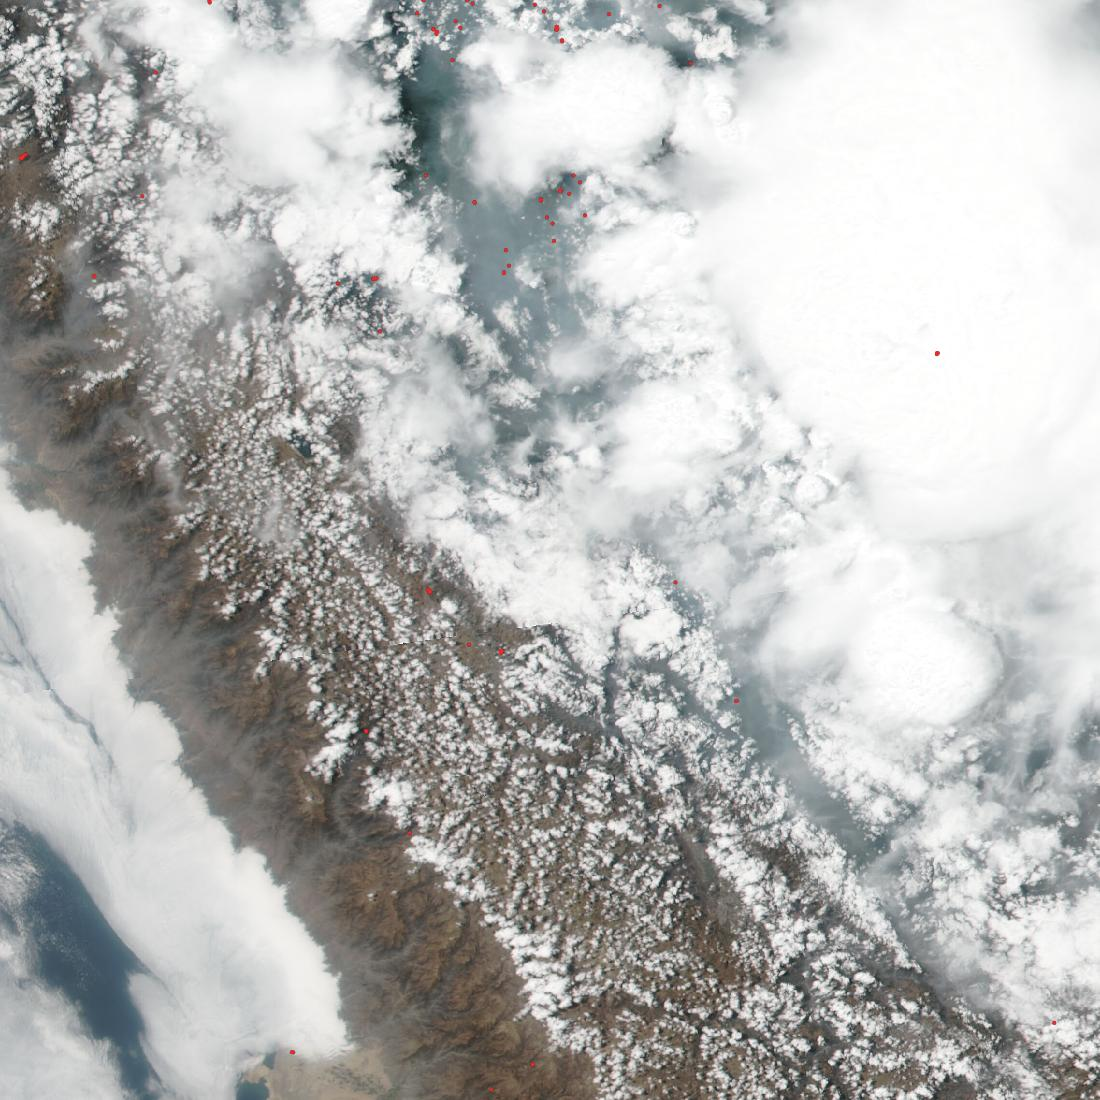
\includegraphics[width=\linewidth]{figuras/wv_viirs.jpg}};
    \begin{scope}[x={(img.south east)},y={(img.north west)}]
      \draw[white,thick] (0.458,0.386) circle (0.022);
      \node[white,fill=black,fill opacity=.75,text opacity=1,inner sep=2pt,font=\footnotesize\bfseries,anchor=west] at (0.49,0.386) {Huancayo};
    \end{scope}
  \end{tikzpicture}
  \caption{VIIRS en Suomi NPP: color verdadero y detecciones de 375~m.}
\end{subfigure}\hfill
\begin{subfigure}[t]{0.485\textwidth}
  \begin{tikzpicture}
    \node[inner sep=0,anchor=south west] (img) at (0,0) {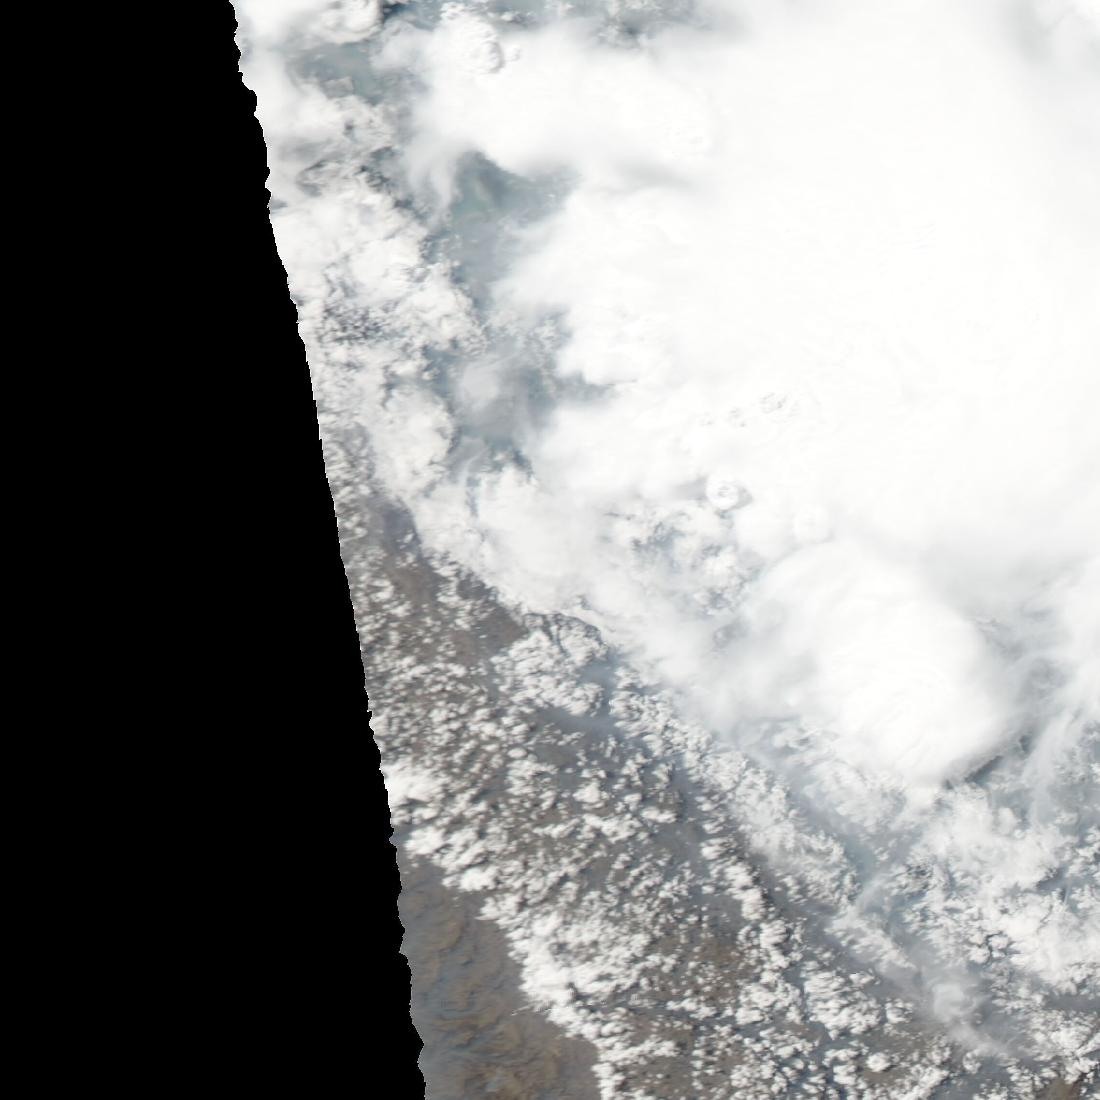
\includegraphics[width=\linewidth]{figuras/wv_modis.jpg}};
    \begin{scope}[x={(img.south east)},y={(img.north west)}]
      \draw[white,thick] (0.458,0.386) circle (0.022);
      \node[white,fill=black,fill opacity=.75,text opacity=1,inner sep=2pt,font=\footnotesize\bfseries,anchor=west] at (0.49,0.386) {Huancayo};
      \node[white,font=\footnotesize,align=center] at (0.17,0.62) {sin datos:\\ fuera de la\\ franja de Aqua};
    \end{scope}
  \end{tikzpicture}
  \caption{MODIS en Aqua: color verdadero y detecciones de 1~km.}
\end{subfigure}
\caption{El centro del Perú el 15 de septiembre de 2024 visto por los dos sensores de la tarde.
Imágenes de NASA Worldview (capas \emph{Corrected Reflectance} y \emph{Fires and Thermal
Anomalies}). El círculo marca la posición de Huancayo.}
\label{fig:worldview}
\end{figure}

Vale la pena mirarlas despacio, porque en un solo par de imágenes aparecen tres de los fenómenos
estudiados hasta aquí.

\textbf{El hueco de MODIS.} Toda la mitad izquierda de la imagen de Aqua está en negro. No es un
fallo: ese día, el borde de la franja de Aqua pasó por el centro del recuadro y la costa y buena
parte de la sierra quedaron en el hueco entre dos órbitas (sección~\ref{sec:huecos}). VIIRS, con
su franja más ancha, cubre el recuadro entero.

\textbf{Las detecciones.} En la imagen de VIIRS se cuentan varias decenas de puntos rojos,
agrupados sobre todo en la selva central, en la parte superior. En la imagen de Aqua no se
distingue ninguno. Parte de esos fuegos caía fuera de la franja de Aqua; los demás estaban en su
borde extremo, donde los píxeles de MODIS miden varios kilómetros
(capítulo~\ref{cap:escaneo}).

\textbf{Las nubes.} Más de la mitad de la escena está cubierta. Todo lo que ardiera bajo la gran
masa nubosa de la derecha es invisible para ambos sensores (capítulo~\ref{cap:atmosfera}). El
humo, en cambio, se aprecia como un velo grisáceo sobre la selva sin impedir las detecciones.

\begin{atencion}[Lo que esta imagen dice y lo que no]
Este es un solo día, elegido porque ilustra bien las diferencias. Otros días la franja de Aqua
cubre la zona de lleno y ambos sensores detectan fuegos. La imagen no demuestra que <<MODIS no
ve nada>>, sino por qué el conteo diario de MODIS en latitudes bajas es irregular y por qué
ninguna comparación entre los sensores debe apoyarse en días sueltos. La comparación válida es
la de muchos días acumulados.
\end{atencion}

\section{El final de MODIS}

Terra y Aqua llevan más de dos décadas en órbita. Sus horas de paso derivan al dejar
de mantenerse sus órbitas nominales; NASA indica que ese cambio debe evaluarse según
el uso científico. No fijamos aquí una fecha definitiva de cierre de ambas misiones:
el plan y el estado deben comprobarse en las fuentes oficiales.\fuente{transition}

La continuidad también afecta a VIIRS. NOAA anunció el fin de entrega de datos de
Suomi NPP el 2 de noviembre de 2026 a las 15:40 UTC.\fuente{noaa-snpp} Sus observaciones
históricas permiten calibrar, pero un sistema que continúe después necesita evaluar
el enlace con NOAA-20 o NOAA-21. Compartir familia instrumental no garantiza igualdad
de calibración, hora exacta ni cobertura. La comparación se repite en su propio solape.

\resumen

\begin{itemize}
  \item \textbf{MODIS} (Terra y Aqua) detecta fuego con píxeles de 1~km usando las bandas 21 y
  22 (3,96~\um) y 31 (11~\um). \textbf{VIIRS} (Suomi NPP, NOAA-20, NOAA-21) lo hace con píxeles
  de 375~m usando I4 (3,74~\um) e I5 (11,45~\um).
  \item Un detector se \textbf{satura} cuando la radiancia supera su máximo. MODIS usa dos
  bandas para cubrir fondo y fuego; la banda I4 de VIIRS se satura a 367~K.
  \item VIIRS cuenta más que MODIS por dos familias de motivos: \emph{ve fuegos que MODIS no ve}
  (píxel pequeño, bordes, huecos) y \emph{cuenta más veces lo mismo} (más píxeles por fuego, más
  satélites).
  \item La razón entre ambos conteos \textbf{no es constante}: depende del tipo de fuego, de la
  región y de la época.
  \item La continuidad exige evaluar tanto la transición MODIS--VIIRS como los cambios
  de plataforma dentro de VIIRS; Suomi NPP ya no aporta datos nuevos tras el cierre anunciado.
\end{itemize}

\ejercicios

\begin{enumerate}
  \item Calcula cuántos píxeles de VIIRS de 375~m caben en un píxel de MODIS, en el nadir y en
  el borde de la franja de MODIS (usa los tamaños de la tabla~\ref{tab:comparacion}).
  \item Para cada fila de la tabla~\ref{tab:comparacion}, indica si la diferencia pertenece a
  la familia <<ve fuegos que el otro no ve>> o a la familia <<cuenta más veces lo mismo>>, o a
  ninguna.
  \item ¿Por qué MODIS necesita dos bandas a 3,96~\um? ¿Qué pasaría si solo tuviera la 22? ¿Y si
  solo tuviera la 21?
  \item Una región tiene casi exclusivamente quemas de rastrojo de menos de una hectárea. Otra
  tiene incendios forestales de miles de hectáreas. ¿En cuál esperas una razón VIIRS/MODIS
  mayor? Justifica con las dos familias de diferencias.
  \item En la figura~\ref{fig:worldview}, ¿qué proporción aproximada del recuadro quedó sin
  observar por Aqua? Si eso ocurre uno de cada seis días, ¿qué fracción de las oportunidades
  diurnas de Aqua se pierde en esa zona por los huecos?
  \item Cuando MODIS se apague, ¿qué parte del ciclo diurno del fuego dejará de observarse? ¿Qué
  tipo de fuego crees que se verá más afectado?
\end{enumerate}

\lecturas

Los dos artículos fundamentales son Giglio, Schroeder y Justice (2016) para el algoritmo de
MODIS, y Schroeder, Oliva, Giglio y Csiszar (2014) para el de VIIRS de 375~m. Las referencias
completas y sus enlaces están en el apéndice~\ref{ap:fuentes}.


\part{Del píxel al foco de calor}
\chapter{Del píxel al foco: cómo se detecta un fuego}\label{cap:deteccion}

\objetivos{
\begin{itemize}
  \item Plantear el modelo del píxel mixto y calcular la temperatura de brillo de un píxel que
  contiene un fuego pequeño.
  \item Explicar por qué el tamaño mínimo detectable es proporcional al área del píxel.
  \item Describir, paso a paso, el algoritmo contextual de detección.
  \item Interpretar el valor de confianza de MODIS y de VIIRS.
\end{itemize}}

\section{El problema}

Un fuego casi nunca llena un píxel. Una quema de rastrojo ocupa unas decenas o centenas de
metros cuadrados dentro de un píxel de un millón. La pregunta de este capítulo es cómo puede un
sensor notar algo que ocupa una diezmilésima parte de lo que está mirando, y cómo decide un
programa, sin intervención humana y para todo el planeta varias veces al día, qué píxeles tienen
fuego.

\section{El píxel mixto}

El detector no distingue las partes del píxel: suma toda la radiación que llega de su huella. Si
una fracción $p$ del área está ocupada por fuego a temperatura $T_f$ y el resto, $1-p$, por un
fondo a temperatura $T_b$, la radiancia que mide en un canal de longitud de onda $\lambda$ es el
promedio ponderado por área:
\begin{equation}\label{eq:mixto}
  L_\lambda = p\,B_\lambda(T_f) + (1-p)\,B_\lambda(T_b).
\end{equation}
Este es el \termino{modelo del píxel mixto} (figura~\ref{fig:mixto}). Supone cuerpos negros y
desprecia la atmósfera, pero recoge lo esencial.

\begin{figure}[ht]
\centering
\begin{tikzpicture}
  \fill[bosque!30] (0,0) rectangle (4.5,4.5);
  \draw[ceniza,thick] (0,0) rectangle (4.5,4.5);
  \shade[inner color=yellow,outer color=fuego] (3.1,1.2) rectangle (3.55,1.65);
  \node[font=\small,align=center] at (2.25,3.75) {fondo\\ $T_b$, fracción $1-p$};
  \draw[<-] (3.33,1.7)--(3.33,2.3) node[above,font=\footnotesize,align=center]{fuego\\ $T_f$, fracción $p$};
  \draw[<->] (0,-0.3)--(4.5,-0.3) node[midway,below,font=\footnotesize]{un píxel};
  \node[font=\Large] at (5.6,2.25) {$\Longrightarrow$};
  \node[caja,align=left,text width=6.3cm,anchor=west] at (6.5,2.25) {%
    El sensor mide una sola radiancia por canal:\\[4pt]
    $L_4 = p\,B_4(T_f) + (1-p)\,B_4(T_b)$\\[2pt]
    $L_{11} = p\,B_{11}(T_f) + (1-p)\,B_{11}(T_b)$\\[4pt]
    y las convierte en dos temperaturas de brillo, $T_4$ y $T_{11}$.};
\end{tikzpicture}
\caption{El modelo del píxel mixto: una pequeña fracción muy caliente dentro de un fondo
uniforme.}
\label{fig:mixto}
\end{figure}

\begin{ejemplo}{un fuego de 100 metros cuadrados en un píxel de MODIS}
Un píxel de \SI{1}{\kilo\metre\squared} con fondo a 300~K contiene un fuego de
\SI{100}{\metre\squared} a 1000~K. Calcula las temperaturas de brillo a 3,96 y a 11~\um.
\solucion La fracción de fuego es $p = 100/10^6 = 10^{-4}$. Con las radiancias del
capítulo~\ref{cap:radiacion} ($B_4$: 0,673 para el fondo y 3320 para el fuego; $B_{11}$: 9,57 y
274):
\begin{align*}
  L_4 &= 10^{-4}\times 3320 + 0{,}9999\times 0{,}673 = 0{,}332 + 0{,}673 = 1{,}005,\\
  L_{11} &= 10^{-4}\times 274 + 0{,}9999\times 9{,}573 = 0{,}027 + 9{,}572 = 9{,}599.
\end{align*}
Convirtiendo con la ecuación~\eqref{eq:tb}: $T_4 = \SI{310.3}{\kelvin}$ y $T_{11} = \SI{300.2}{\kelvin}$.

Un fuego que ocupa una diezmilésima del píxel sube la temperatura de brillo a 4~\um{} en
\textbf{10 kelvin} y la de 11~\um{} en apenas \textbf{0,2 kelvin}. A 4~\um, la contribución del
fuego (0,332) es la mitad de la del fondo entero (0,673).
\end{ejemplo}

La figura~\ref{fig:mixto-curvas} generaliza el ejemplo a cualquier fracción de fuego.

\begin{figure}[ht]
\centering
\begin{tikzpicture}
\begin{axis}[width=13cm,height=7.2cm,xmode=log,xmin=1e-5,xmax=1e-1,ymin=295,ymax=520,
  xlabel={Fracción del píxel ocupada por fuego a 1000 K},
  ylabel={Temperatura de brillo del píxel (K)},
  legend style={at={(0.5,1.04)},anchor=south,font=\small,draw=none,legend columns=2,
    /tikz/every even column/.append style={column sep=10pt}},
  grid=major,grid style={ceniza!15},samples=120,domain=1e-5:1e-1,
  declare function={
    planck(\l,\T)=1.191e8/(\l^5*(exp(14388/(\l*\T))-1));
    tb(\l,\L)=14388/(\l*ln(1+1.191e8/(\l^5*\L)));}]
\addplot[fuego,very thick] {tb(3.96, x*planck(3.96,1000)+(1-x)*planck(3.96,300))};
\addplot[cielo,very thick] {tb(11, x*planck(11,1000)+(1-x)*planck(11,300))};
\legend{$T_4$ (3{,}96~\um),$T_{11}$ (11~\um)}
\draw[ceniza,dashed] (axis cs:1e-4,295)--(axis cs:1e-4,520);
\draw[ceniza,dashed] (axis cs:1e-3,295)--(axis cs:1e-3,520);
\node[font=\footnotesize,rotate=90,anchor=south east] at (axis cs:1e-4,518) {100 m$^2$ en 1 km$^2$};
\node[font=\footnotesize,rotate=90,anchor=south east] at (axis cs:1e-3,518) {1000 m$^2$ en 1 km$^2$};
\draw[<->,thick] (axis cs:1e-3,301.9)--(axis cs:1e-3,351.7);
\node[font=\footnotesize,anchor=west,fill=white,inner sep=1pt] at (axis cs:1.15e-3,327) {$\Delta T \approx 50$ K};
\end{axis}
\end{tikzpicture}
\caption{Temperaturas de brillo de un píxel con fondo a 300~K según la fracción ocupada por un
fuego a 1000~K, calculadas con las ecuaciones~\eqref{eq:mixto} y~\eqref{eq:tb}. El canal de
4~\um{} reacciona a fracciones minúsculas; el de 11~\um{} casi no se entera hasta que el fuego
ocupa cerca del 1\,{}\% del píxel.}
\label{fig:mixto-curvas}
\end{figure}

Dos conclusiones de la figura.

\textbf{La firma del fuego es la separación entre los dos canales.} Un píxel sin fuego tiene
$T_4$ y $T_{11}$ parecidas (de día, $T_4$ es algo mayor por la luz solar reflejada). Un píxel
con fuego tiene $T_4$ mucho mayor que $T_{11}$. Por eso la variable clave es
\begin{equation}
  \Delta T = T_4 - T_{11}.
\end{equation}

\textbf{Dos incógnitas, dos ecuaciones.} El modelo tiene dos incógnitas del fuego, $p$ y $T_f$,
y dos mediciones, $L_4$ y $L_{11}$. En principio pueden despejarse el tamaño y la temperatura
del fuego. Es el \emph{método biespectral}, propuesto por Dozier en 1981. En la práctica es muy
sensible a los errores (como el canal de 11~\um{} apenas cambia, cualquier imprecisión en el
fondo arruina la solución) y no se usa para producir los datos habituales, pero es el origen
conceptual de todo el campo.

\section{El tamaño mínimo detectable depende del píxel}

Supón que el algoritmo exige que $T_4$ supere al fondo en cierto margen, digamos 10~K. Para un
fondo a 300~K eso equivale a que la radiancia a 4~\um{} suba de 0,673 a 1,00, es decir, un
exceso de $\Delta L = 0{,}33$ unidades. Del modelo del píxel mixto, despreciando $p$ frente a 1:
\begin{equation}
  \Delta L \approx p\,B_4(T_f)
  \quad\Longrightarrow\quad
  p_{\min} \approx \frac{\Delta L}{B_4(T_f)} .
\end{equation}
La \emph{fracción} mínima no depende del tamaño del píxel. Pero el \emph{área} mínima del fuego
sí:
\begin{equation}\label{eq:amin}
  A_{\min} = p_{\min}\times A_{\text{píxel}} .
\end{equation}

\begin{definicion}{tamaño mínimo detectable}
El tamaño mínimo detectable es el área del fuego más pequeño que produce una anomalía
suficiente para que el algoritmo lo acepte. Es proporcional al área del píxel y depende
fuertemente de la temperatura del fuego y de las condiciones del fondo.
\end{definicion}

\begin{ejemplo}{el mismo fuego en MODIS y en VIIRS}
Con el criterio de 10~K sobre un fondo a 300~K, calcula el área mínima detectable de un fuego a
1000~K y de una brasa a 600~K para: (a) un píxel de MODIS en el nadir, 1~km$^2$; (b) un píxel de
MODIS en el borde, $2{,}0\times4{,}8$~km; (c) un píxel de VIIRS en el nadir, $375\times375$~m.
\solucion Las fracciones mínimas son $p_{\min} = 0{,}33/3320 = \num{1.0e-4}$ para 1000~K y
$p_{\min} = 0{,}33/287{,}5 = \num{1.1e-3}$ para 600~K (con $B_4(600) = 287{,}5$). Multiplicando
por el área de cada píxel:
\begin{center}
\begin{tabular}{lrrr}
\toprule
Píxel & Área & Fuego a 1000 K & Brasa a 600 K \\
\midrule
MODIS, nadir & \SI{1.0}{\kilo\metre\squared} & \SI{100}{\metre\squared} & \SI{1100}{\metre\squared} \\
MODIS, borde & \SI{9.6}{\kilo\metre\squared} & \SI{960}{\metre\squared} & \SI{11000}{\metre\squared} \\
VIIRS, nadir & \SI{0.14}{\kilo\metre\squared} & \SI{14}{\metre\squared} & \SI{160}{\metre\squared} \\
\bottomrule
\end{tabular}
\end{center}
Un fuego de \SI{50}{\metre\squared} a 1000~K (una quema de 7 por 7 metros) es detectable por
VIIRS y no por MODIS. Y una brasa a 600~K necesita ser diez veces más extensa que una llama a
1000~K para detectarse.
\end{ejemplo}

\begin{atencion}[Estos números son ilustrativos]
El criterio real no es un umbral fijo de 10~K sino un conjunto de pruebas, y el umbral efectivo
cambia con la variabilidad del fondo, la hora y la geometría. Los valores de la tabla sirven
para comparar sensores, no como especificación. Lo que sí es sólido es la proporcionalidad de la
ecuación~\eqref{eq:amin}.
\end{atencion}

\begin{parareto}
La ecuación~\eqref{eq:amin} es la explicación física, en una línea, de por qué VIIRS detecta más
que MODIS, y por qué la diferencia es mayor para quemas pequeñas y de baja temperatura. Es un
buen argumento para el pitch: la razón VIIRS/MODIS \emph{tiene que} depender del tipo de fuego,
porque depende de cuántos fuegos caen entre los dos límites de detección.
\end{parareto}

\section{El algoritmo contextual}

Detectar un fuego sería sencillo si el fondo fuera siempre igual: bastaría un umbral fijo. Pero
el fondo va desde un glaciar a 260~K hasta un desierto a 330~K, y de día la luz reflejada lo
altera todo. Un umbral único daría miles de falsas alarmas en el Sahara y dejaría pasar la
mayoría de los fuegos de Siberia.

La solución es comparar cada píxel con sus vecinos.

\begin{definicion}{algoritmo contextual}
Un algoritmo contextual decide si un píxel contiene fuego comparando sus temperaturas de brillo
con las de los píxeles de su entorno, que se toman como estimación de cómo se vería ese píxel
si no ardiera.
\end{definicion}

El algoritmo de MODIS procesa cada píxel en la secuencia de la figura~\ref{fig:algoritmo}. El de
VIIRS de 375~m sigue el mismo esquema con las bandas I4 e I5 y umbrales adaptados.

\begin{figure}[ht]
\centering
\begin{tikzpicture}[node distance=7mm,
  paso/.style={caja,text width=5.6cm,fill=cieloClaro},
  fin/.style={caja,fill=cenizaClaro,text width=2.9cm},
  si/.style={caja,fill=fuegoClaro,text width=2.9cm,font=\small\bfseries}]
  \node[paso] (a) {\textbf{1. Máscaras}\\ ¿es nube o agua?};
  \node[paso,below=of a] (b) {\textbf{2. Candidato}\\ ¿$T_4$ y $\Delta T$ superan un mínimo?};
  \node[paso,below=of b] (c) {\textbf{3. Prueba absoluta}\\ ¿$T_4$ es altísima?};
  \node[paso,below=of c] (d) {\textbf{4. Fondo}\\ estadísticas de los vecinos válidos};
  \node[paso,below=of d] (e) {\textbf{5. Pruebas contextuales}\\ ¿destaca sobre su fondo?};
  \node[paso,below=of e] (f) {\textbf{6. Rechazos}\\ ¿brillo solar, desierto, costa?};
  \node[si,below=of f] (g) {FUEGO\\ + confianza};
  \node[fin,right=14mm of a] (a2) {descartado};
  \node[fin,right=14mm of b] (b2) {sin fuego};
  \node[fin,right=14mm of e] (e2) {sin fuego};
  \node[fin,right=14mm of f] (f2) {sin fuego};
  \node[fin,right=14mm of d] (d2) {<<desconocido>>};
  \draw[flujo] (a)--(b) node[midway,left,font=\footnotesize]{no};
  \draw[flujo] (b)--(c) node[midway,left,font=\footnotesize]{sí};
  \draw[flujo] (c)--(d) node[midway,left,font=\footnotesize]{no};
  \draw[flujo] (d)--(e);
  \draw[flujo] (e)--(f) node[midway,left,font=\footnotesize]{sí};
  \draw[flujo] (f)--(g) node[midway,left,font=\footnotesize]{no};
  \draw[flujo] (a)--(a2) node[midway,above,font=\footnotesize]{sí};
  \draw[flujo] (b)--(b2) node[midway,above,font=\footnotesize]{no};
  \draw[flujo] (e)--(e2) node[midway,above,font=\footnotesize]{no};
  \draw[flujo] (f)--(f2) node[midway,above,font=\footnotesize]{sí};
  \draw[flujo] (d)--(d2) node[midway,above,font=\footnotesize,align=center]{pocos\\[-2pt] vecinos};
  \draw[flujo] (c.west) -- ++(-1.0,0) |- (f.west) node[pos=0.25,left,font=\footnotesize]{sí};
\end{tikzpicture}
\caption{Esquema del algoritmo contextual de detección de fuego activo.}
\label{fig:algoritmo}
\end{figure}

\subsection{Paso 1: máscaras de nubes y de agua}

Los píxeles nubosos se identifican con pruebas sencillas de reflectancia y de temperatura: una
nube es muy brillante en el visible y fría a 12~\um. Los píxeles de agua se toman de un mapa
fijo. Ninguno de los dos se evalúa como posible fuego ni se usa como vecino <<de fondo>>.

\subsection{Paso 2: candidatos}

Para no gastar cálculo en los millones de píxeles que evidentemente no arden, se descartan los
que no alcanzan unos mínimos muy permisivos. En MODIS, de día, un píxel es
\termino{candidato a fuego} si
\begin{equation}
  T_4 > \SI{310}{\kelvin}, \qquad \Delta T > \SI{10}{\kelvin}, \qquad \rho_{0{,}86} < 0{,}3,
\end{equation}
donde $\rho_{0{,}86}$ es la reflectancia en el infrarrojo cercano (un valor alto delata nube o
brillo solar). De noche, el umbral de $T_4$ baja a 305~K y no se usa la reflectancia.

\subsection{Paso 3: prueba absoluta}

Si el píxel está tan caliente que no cabe otra explicación, se acepta sin mirar el entorno. En
MODIS: $T_4 > \SI{360}{\kelvin}$ de día o $T_4 > \SI{320}{\kelvin}$ de noche.

\subsection{Paso 4: caracterización del fondo}

Para el resto de candidatos se abre una ventana cuadrada centrada en el píxel y se reúnen los
vecinos \termino{válidos}: los que no son nube, ni agua, ni a su vez posibles fuegos. La ventana
empieza pequeña y crece (hasta $21\times21$ píxeles en MODIS) hasta juntar al menos una cuarta
parte de vecinos válidos y un mínimo de ocho. Si ni así se consigue, el píxel queda clasificado
como <<desconocido>> (figura~\ref{fig:ventana}).

Con los vecinos válidos se calculan la media y una medida de dispersión de $T_4$, de $T_{11}$ y
de $\Delta T$. Se usa la \termino{desviación absoluta media}, $\delta$, que es el promedio de
las distancias de cada valor a la media; es menos sensible a valores extremos que la desviación
estándar. Llamaremos $\overline{T_4}$, $\delta_4$, $\overline{\Delta T}$ y $\delta_{\Delta T}$ a
los valores del fondo.

\begin{figure}[ht]
\centering
\begin{tikzpicture}[x=0.62cm,y=0.62cm]
  \foreach \i in {0,...,8}{\foreach \j in {0,...,8}{\fill[bosque!22] (\i,\j) rectangle ++(1,1);}}
  \foreach \i/\j in {0/8,1/8,2/8,0/7,1/7,2/7,3/8,0/6,1/6}{\fill[white] (\i,\j) rectangle ++(1,1);}
  \foreach \i/\j in {6/0,7/0,8/0,7/1,8/1,8/2}{\fill[cielo!45] (\i,\j) rectangle ++(1,1);}
  \foreach \i/\j in {5/4,5/5,3/3}{\fill[brasa!60] (\i,\j) rectangle ++(1,1);}
  \fill[fuego] (4,4) rectangle ++(1,1);
  \foreach \i in {0,...,9}{\draw[ceniza!70,thin] (\i,0)--(\i,9); \draw[ceniza!70,thin] (0,\i)--(9,\i);}
  \draw[black,very thick] (4,4) rectangle ++(1,1);
  \draw[black,thick,dashed] (2,2) rectangle (7,7);
  \begin{scope}[shift={(10.3,7.6)}]
    \fill[fuego] (0,0) rectangle ++(0.7,0.7); \node[right,font=\footnotesize] at (0.9,0.35) {píxel que se evalúa};
    \fill[bosque!22] (0,-1.1) rectangle ++(0.7,0.7); \node[right,font=\footnotesize] at (0.9,-0.75) {vecino válido (fondo)};
    \fill[brasa!60] (0,-2.2) rectangle ++(0.7,0.7); \node[right,font=\footnotesize] at (0.9,-1.85) {otro posible fuego: excluido};
    \fill[white] (0,-3.3) rectangle ++(0.7,0.7); \draw[ceniza] (0,-3.3) rectangle ++(0.7,0.7); \node[right,font=\footnotesize] at (0.9,-2.95) {nube: excluida};
    \fill[cielo!45] (0,-4.4) rectangle ++(0.7,0.7); \node[right,font=\footnotesize] at (0.9,-4.05) {agua: excluida};
    \draw[black,thick,dashed] (0,-5.5) rectangle ++(0.7,0.7); \node[right,font=\footnotesize] at (0.9,-5.15) {ventana actual ($5\times5$)};
  \end{scope}
\end{tikzpicture}
\caption{Ventana de fondo. Solo los vecinos válidos entran en las estadísticas. Si no hay
suficientes, la ventana se agranda.}
\label{fig:ventana}
\end{figure}

\subsection{Paso 5: pruebas contextuales}

El candidato se acepta como fuego si destaca de su fondo en las dos variables. Las condiciones
centrales del algoritmo de MODIS son
\begin{align}
  \Delta T &> \overline{\Delta T} + 3{,}5\,\delta_{\Delta T}, \label{eq:ctx1}\\
  \Delta T &> \overline{\Delta T} + \SI{6}{\kelvin}, \label{eq:ctx2}\\
  T_4 &> \overline{T_4} + 3\,\delta_4 . \label{eq:ctx3}
\end{align}
La primera y la tercera son relativas: exigen que el píxel se aparte de la media varias veces lo
que suelen apartarse sus vecinos. En un entorno homogéneo ($\delta$ pequeña) basta una anomalía
modesta; en uno heterogéneo se exige más. La segunda impone un mínimo absoluto de 6~K para que,
en fondos extremadamente uniformes, una diferencia insignificante no dispare una detección. De
día hay condiciones adicionales sobre el canal de 11~\um.

\begin{ejemplo}{aplicar las pruebas contextuales}
Un píxel diurno tiene $T_4 = \SI{318.0}{\kelvin}$ y $T_{11} = \SI{299.5}{\kelvin}$. Sus vecinos
válidos tienen $\overline{T_4} = \SI{304.0}{\kelvin}$, $\delta_4 = \SI{1.8}{\kelvin}$,
$\overline{\Delta T} = \SI{5.5}{\kelvin}$ y $\delta_{\Delta T} = \SI{1.2}{\kelvin}$. ¿Es fuego?
\solucion $\Delta T = 318{,}0 - 299{,}5 = \SI{18.5}{\kelvin}$. Es candidato: $T_4 > 310$ y
$\Delta T > 10$. No pasa la prueba absoluta ($318 < 360$). Pruebas contextuales:
\begin{itemize}
  \item \eqref{eq:ctx1}: $5{,}5 + 3{,}5\times1{,}2 = 9{,}7$; $18{,}5 > 9{,}7$. Se cumple.
  \item \eqref{eq:ctx2}: $5{,}5 + 6 = 11{,}5$; $18{,}5 > 11{,}5$. Se cumple.
  \item \eqref{eq:ctx3}: $304{,}0 + 3\times1{,}8 = 309{,}4$; $318{,}0 > 309{,}4$. Se cumple.
\end{itemize}
El píxel se clasifica como fuego, salvo que lo rechace alguna prueba del paso 6.

Si el mismo píxel estuviera en un paisaje muy heterogéneo con $\delta_{\Delta T} =
\SI{4.5}{\kelvin}$, la primera condición exigiría $\Delta T > 5{,}5 + 15{,}75 = 21{,}3$~K y el
píxel \emph{no} sería fuego. El mismo fuego se detecta o no según cómo sea su entorno.
\end{ejemplo}

\subsection{Paso 6: rechazo de falsas alarmas}

Por último se descartan las detecciones diurnas que coinciden con las situaciones del
capítulo~\ref{cap:atmosfera}: geometría de brillo solar, límites de desierto (cuando muchos
vecinos quedaron excluidos por ser candidatos sin serlo realmente) y bordes de costa.

\section{Confianza}

Cada detección lleva una estimación de cuán segura es.

En \textbf{MODIS} es un número entre 0 y 100. Se calcula combinando cuánto supera el píxel los
umbrales: qué tan alto es $T_4$, cuántas desviaciones se aparta del fondo en $T_4$ y en
$\Delta T$, y cuántos vecinos son nube o agua. Por convención se agrupa en tres clases:
\emph{baja} (menos de 30), \emph{nominal} (de 30 a 80) y \emph{alta} (más de 80).

En \textbf{VIIRS} de 375~m es directamente una de tres categorías:
\begin{itemize}
  \item \emph{low} (\texttt{l}): detecciones diurnas en zona de posible brillo solar o con una
  anomalía térmica débil;
  \item \emph{nominal} (\texttt{n}): detecciones sin esas circunstancias y con una anomalía
  clara;
  \item \emph{high} (\texttt{h}): píxeles saturados, de día o de noche.
\end{itemize}

\begin{atencion}[La confianza no es una probabilidad y no es comparable entre sensores]
Un valor de 70 en MODIS no significa <<70\,{}\% de probabilidad de ser fuego>>. Y la clase <<alta>>
de VIIRS (píxel saturado) no equivale a la clase <<alta>> de MODIS (número mayor que 80). Si
filtras por confianza, define el filtro por separado para cada sensor y mantén ese criterio fijo
en todo el periodo. Un criterio habitual y fácil de defender: descartar solo la clase baja en
ambos.
\end{atencion}

\section{Diferencias del algoritmo de VIIRS}

El algoritmo de 375~m hereda el esquema de MODIS, con adaptaciones a su instrumento:

\begin{itemize}
  \item usa I4 (3,74~\um) e I5 (11,45~\um), más las bandas I1 a I3 para nubes, agua y brillo
  solar;
  \item como I4 se satura a 367~K, trata de forma especial los píxeles saturados, e incluso los
  casos en que la saturación extrema produce valores anómalamente bajos;
  \item ajusta sus umbrales de candidatura según las condiciones de la escena;
  \item presta atención a la región de la Anomalía del Atlántico Sur, donde la radiación del
  espacio produce ruido en el detector que puede simular fuegos nocturnos. Esa región incluye
  buena parte de Sudamérica.
\end{itemize}

El resultado es un producto con errores de comisión bajos (del orden del 1\,{}\% para la clase
nominal en la evaluación inicial) y una sensibilidad a fuegos pequeños muy superior a la de
MODIS, sobre todo de noche.

\resumen

\begin{itemize}
  \item El \textbf{modelo del píxel mixto} combina fuego y fondo ponderados por área:
  $L = p\,B(T_f) + (1-p)\,B(T_b)$.
  \item Un fuego de 100~m$^2$ a 1000~K en un píxel de 1~km$^2$ eleva $T_4$ unos 10~K y $T_{11}$
  unos 0,2~K. La firma del fuego es $\Delta T = T_4 - T_{11}$.
  \item El \textbf{área mínima detectable} es proporcional al área del píxel: unas siete veces
  menor en VIIRS que en MODIS en el nadir, y la diferencia crece hacia los bordes.
  \item El \textbf{algoritmo contextual} filtra nubes y agua, selecciona candidatos, caracteriza
  el fondo con los vecinos válidos y acepta el píxel si destaca varias desviaciones sobre él.
  \item Que un fuego se detecte depende también de la homogeneidad de su entorno.
  \item La \textbf{confianza} es un número de 0 a 100 en MODIS y una categoría en VIIRS. No son
  equivalentes.
\end{itemize}

\ejercicios

\begin{enumerate}
  \item Repite el primer ejemplo del capítulo para un fuego de \SI{1000}{\metre\squared} a
  800~K ($B_4(800) = 1317$, $B_{11}(800) = 179$). Obtén $T_4$, $T_{11}$ y $\Delta T$.
  \item ¿Qué fracción de un píxel debe ocupar un fuego a 1000~K para \emph{saturar} la banda I4
  de VIIRS (367~K) con fondo a 300~K? Exprésala como área dentro de un píxel de
  $375\times375$~m. Pista: calcula primero la radiancia de un cuerpo negro a 367~K en
  3,74~\um.
  \item Usando la ecuación~\eqref{eq:amin}, ¿cuánto mayor es el fuego mínimo detectable por
  MODIS a 900~km del nadir (píxel de unos $1{,}7\times3{,}1$~km) que en el nadir?
  \item Un píxel nocturno tiene $T_4 = \SI{309}{\kelvin}$, $T_{11} = \SI{287}{\kelvin}$, y su
  fondo $\overline{T_4} = \SI{289}{\kelvin}$, $\delta_4 = \SI{0.9}{\kelvin}$,
  $\overline{\Delta T} = \SI{1.5}{\kelvin}$, $\delta_{\Delta T} = \SI{0.6}{\kelvin}$. Aplica los
  pasos 2, 3 y 5.
  \item Explica por qué se excluyen del fondo los vecinos que son a su vez candidatos a fuego.
  ¿Qué le pasaría a la detección en el centro de un incendio grande si no se excluyeran?
  \item Dos quemas idénticas ocurren a la vez: una en una pampa uniforme y otra en un mosaico de
  chacras, eriazos y bosque. ¿Cuál tiene más probabilidad de ser detectada? ¿Qué implica esto
  para comparar el número de focos entre dos paisajes distintos?
  \item ¿Por qué no es correcto filtrar <<confianza $\geq 50$>> en un archivo que mezcla
  detecciones de MODIS y de VIIRS?
\end{enumerate}

\lecturas

Giglio, Descloitres, Justice y Kaufman (2003) describen el algoritmo contextual original de
MODIS, y Giglio, Schroeder y Justice (2016) su versión actual (Colección~6). Schroeder y
colaboradores (2014) presentan el algoritmo de VIIRS de 375~m. Véase el
apéndice~\ref{ap:fuentes}.

\chapter{Potencia radiativa del fuego}\label{cap:frp}

\objetivos{
\begin{itemize}
  \item Definir la potencia radiativa del fuego (FRP) y explicar qué mide físicamente.
  \item Entender por qué puede estimarse con un solo canal de 4~\um.
  \item Relacionar la FRP con la biomasa consumida y con las emisiones.
  \item Explicar cómo se calcula en MODIS y en VIIRS y qué precauciones exige al comparar.
\end{itemize}}

\section{Más allá de contar}

Un foco dice <<aquí hay fuego>>. No dice cuánto. Una quema de rastrojo y el frente de un incendio
forestal generan cada uno un punto en el mapa. Para distinguirlos, los productos de fuego
incluyen una medida de intensidad.

\begin{definicion}{potencia radiativa del fuego (FRP)}
La potencia radiativa del fuego, o FRP por \emph{Fire Radiative Power}, es la energía que el
fuego contenido en un píxel emite en forma de radiación por unidad de tiempo, sumada sobre todas
las longitudes de onda y todas las direcciones. Se expresa en megavatios (MW).
\end{definicion}

Es la columna \texttt{frp} de los datos. Un megavatio es un millón de vatios; una quema agrícola
pequeña tiene una FRP de unos pocos MW, y los píxeles más intensos de un gran incendio forestal
superan los 1000~MW.

\section{De la ley de Stefan--Boltzmann a la FRP}

Si conociéramos el área $A_f$ y la temperatura $T_f$ del fuego, su potencia radiada saldría de
la ley de Stefan--Boltzmann, restando lo que esa misma superficie emitiría si estuviera a la
temperatura del fondo:
\begin{equation}\label{eq:frp-sb}
  \mathrm{FRP} = \sigma\,A_f\,\bigl(T_f^4 - T_b^4\bigr) \approx \sigma\,A_f\,T_f^4 .
\end{equation}
El término del fondo es despreciable: $300^4$ es menos del 1\,{}\% de $1000^4$.

\begin{ejemplo}{potencia de una quema pequeña}
Calcula la FRP de un fuego de \SI{100}{\metre\squared} a 1000~K y la de uno de
\SI{2000}{\metre\squared} a 800~K.
\solucion Para el primero: $\sigma A_f T_f^4 = \num{5.67e-8}\times 100\times 10^{12} =
\SI{5.67e6}{\watt} = \SI{5.7}{\mega\watt}$. Para el segundo: $\num{5.67e-8}\times 2000\times
(800)^4 = \num{5.67e-8}\times2000\times\num{4.096e11} = \SI{4.6e7}{\watt} =
\SI{46}{\mega\watt}$.
\end{ejemplo}

El problema es que ni $A_f$ ni $T_f$ se conocen: son justamente las incógnitas difíciles de
despejar del capítulo anterior. Se necesita un atajo.

\section{El atajo: en 4 micrómetros, la radiancia va como la cuarta potencia}

El atajo es una coincidencia afortunada de la ley de Planck. En el intervalo de temperaturas de
los fuegos de vegetación, entre unos 600 y 1500~K, la radiancia a 4~\um{} es casi exactamente
proporcional a $T^4$:
\begin{equation}\label{eq:aprox-mir}
  B_4(T) \approx a\,T^4 ,
\end{equation}
con una constante $a$ que depende de la banda concreta del sensor (para MODIS, $a \approx
\SI{3.0e-9}{\watt\per\square\metre\per\steradian\per\micro\metre\per\kelvin\tothe{4}}$).

La figura~\ref{fig:mir} lo comprueba. No es una ley exacta sino una aproximación válida en ese
intervalo, y funciona porque, para esas temperaturas, el canal de 4~\um{} está cerca del máximo
de la curva de Planck.

\begin{figure}[ht]
\centering
\begin{tikzpicture}
\begin{axis}[width=12.5cm,height=6.8cm,xmin=400,xmax=1600,ymin=0,ymax=2,
  xlabel={Temperatura del fuego (K)},
  ylabel={$B_4(T)\,/\,(a\,T^4)$},
  ytick={0,0.5,1,1.5,2},yticklabels={0,{0,5},1,{1,5},2},
  grid=major,grid style={ceniza!15},samples=120,domain=400:1600,
  declare function={planck(\l,\T)=1.191e8/(\l^5*(exp(14388/(\l*\T))-1));}]
\fill[bosque!15] (axis cs:600,0) rectangle (axis cs:1500,2);
\addplot[fuego,very thick] {planck(3.96,x)/(3.0e-9*x^4)};
\addplot[ceniza,dashed,domain=400:1600] {1};
\node[font=\footnotesize,bosque!70!black] at (axis cs:1050,1.75) {intervalo de los fuegos de vegetación};
\end{axis}
\end{tikzpicture}
\caption{Cociente entre la radiancia de Planck a 3,96~\um{} y la aproximación $a\,T^4$. Entre
600 y 1500~K (banda sombreada) el cociente se mantiene entre 0,74 y 1,07: con un error de
hasta un 25\,{}\% en los extremos, la radiancia del canal es proporcional a la potencia total
emitida.}
\label{fig:mir}
\end{figure}

Ahora combinemos tres ecuaciones. El exceso de radiancia del píxel sobre su fondo, según el
modelo del píxel mixto, es $\Delta L_4 = L_4 - L_{4,b} \approx p\,B_4(T_f)$. Con la
aproximación~\eqref{eq:aprox-mir}, $\Delta L_4 \approx p\,a\,T_f^4$. Y como $p =
A_f/A_{\text{píxel}}$:
\[
  \Delta L_4 \approx \frac{A_f}{A_{\text{píxel}}}\,a\,T_f^4
  \quad\Longrightarrow\quad
  A_f\,T_f^4 \approx \frac{A_{\text{píxel}}}{a}\,\Delta L_4 .
\]
Sustituyendo en la ecuación~\eqref{eq:frp-sb}:
\begin{equation}\label{eq:frp-mir}
  \boxed{\;\mathrm{FRP} \approx \frac{\sigma\,A_{\text{píxel}}}{a}\,\bigl(L_4 - L_{4,b}\bigr)\;}
\end{equation}

El producto desconocido $A_f T_f^4$ ha desaparecido. La potencia del fuego se obtiene de tres
cosas que sí se conocen: el área del píxel, la radiancia medida a 4~\um{} y la radiancia del
fondo estimada con los vecinos. Este es el \termino{método de la radiancia en el infrarrojo
medio}, debido a Wooster y colaboradores, y es el que usan los productos actuales.

\begin{ejemplo}{comprobación del método}
Verifica la ecuación~\eqref{eq:frp-mir} con el fuego de \SI{100}{\metre\squared} a 1000~K
dentro de un píxel de \SI{1}{\kilo\metre\squared}, usando los valores del capítulo anterior.
\solucion Allí se obtuvo $L_4 = 1{,}005$ con fondo $L_{4,b} = 0{,}673$, es decir, $\Delta L_4 =
0{,}332$ \si{\watt\per\square\metre\per\steradian\per\micro\metre}. Entonces
\[
 \mathrm{FRP} \approx \frac{\num{5.67e-8}\times 10^6}{\num{3.0e-9}}\times 0{,}332
 = \num{1.89e7}\times 0{,}332 = \SI{6.3e6}{\watt} = \SI{6.3}{\mega\watt}.
\]
El valor exacto del ejemplo anterior era 5,7~MW. La diferencia, de un 10\,{}\%, es el error de la
aproximación~\eqref{eq:aprox-mir} a 1000~K, visible en la figura~\ref{fig:mir}.
\end{ejemplo}

\section{Qué mide y qué no mide la FRP}

La FRP es una potencia: energía por unidad de tiempo en el instante de la pasada. Tres
precisiones.

\textbf{Es solo la parte radiada.} Un fuego libera energía también por convección (el aire
caliente que sube) y por conducción hacia el suelo. La fracción radiada es del orden de una
décima a una quinta parte del total.

\textbf{Es proporcional al ritmo de combustión.} Experimentos de quema controlada muestran que
la energía radiada total es proporcional a la masa de vegetación consumida, con un factor
cercano a 0,37~kg de biomasa seca por megajulio radiado. Por eso la FRP, integrada en el tiempo,
se usa para estimar cuánta biomasa se quemó y cuánto humo y CO$_2$ se emitió.

\textbf{Es instantánea.} Para pasar de potencia a energía hay que integrar sobre la duración del
fuego, y un satélite polar solo aporta unas pocas muestras al día. La integral, llamada
\termino{energía radiativa del fuego} (FRE), requiere suponer la forma del ciclo diurno.

\begin{ejemplo}{de potencia a biomasa}
Un píxel muestra una FRP de 40~MW. Suponiendo que el fuego mantiene esa potencia durante dos
horas, ¿cuánta biomasa consume?
\solucion La energía radiada es $E = \SI{40}{\mega\watt}\times\SI{7200}{\second} =
\SI{2.88e5}{\mega\joule}$. Con 0,37~kg por megajulio: $m = \num{2.88e5}\times 0{,}37 \approx
\SI{1.1e5}{\kilo\gram}$, unas 107 toneladas de materia seca. El resultado depende por completo
de la suposición sobre la duración.
\end{ejemplo}

\section{La FRP en MODIS y en VIIRS}

Los dos productos calculan la FRP con la ecuación~\eqref{eq:frp-mir}, pero con diferencias
importantes en los detalles.

\textbf{MODIS} usa su canal de 3,96~\um{} (banda 22, o 21 si la 22 se satura) y el área real del
píxel, que crece hacia los bordes. La versión actual del producto adoptó este método; las
versiones antiguas usaban una fórmula empírica distinta, basada en la octava potencia de la
temperatura de brillo.

\textbf{VIIRS de 375~m} no puede usar I4 porque se satura a 367~K. La detección se hace a
375~m, pero la FRP se calcula con la radiancia de la banda \textbf{M13}, de 750~m y con un rango
dinámico muy amplio, que no se satura con los fuegos de vegetación. La potencia obtenida para el
píxel de 750~m se reparte entre las detecciones de 375~m que contiene.

\begin{figure}[ht]
\centering
\begin{tikzpicture}[x=1.15cm,y=1.15cm]
  \fill[cenizaClaro] (0,0) rectangle (2,2);
  \draw[ceniza,very thick] (0,0) rectangle (2,2);
  \draw[ceniza] (1,0)--(1,2) (0,1)--(2,1);
  \fill[fuego!60] (0,1) rectangle (1,2); \fill[fuego!60] (1,1) rectangle (2,2); \fill[fuego!60] (1,0) rectangle (2,1);
  \draw[ceniza,very thick] (0,0) rectangle (2,2);
  \draw[ceniza] (1,0)--(1,2) (0,1)--(2,1);
  \node[font=\footnotesize] at (0.5,1.5) {foco}; \node[font=\footnotesize] at (1.5,1.5) {foco}; \node[font=\footnotesize] at (1.5,0.5) {foco};
  \draw[<->] (0,-0.25)--(2,-0.25) node[midway,below,font=\footnotesize]{píxel M13 de 750 m};
  \draw[<->] (2.25,1)--(2.25,2) node[midway,right,font=\footnotesize]{375 m};
  \node[caja,anchor=west,text width=7cm,align=left] at (4.2,1) {%
    FRP medida en el píxel de 750 m: 36 MW\\[3pt]
    Detecciones de 375 m dentro: 3\\[3pt]
    FRP asignada a cada foco: $36/3 = 12$ MW};
\end{tikzpicture}
\caption{En el producto de 375~m de VIIRS, la FRP se mide en la banda M13 de 750~m y se reparte
por igual entre los focos de 375~m contenidos en ese píxel.}
\label{fig:m13}
\end{figure}

\section{Precauciones al usar la FRP}

\begin{atencion}[La FRP de un foco no es comparable sin más entre sensores]
Hay al menos cuatro motivos.
\begin{enumerate}
  \item \textbf{Fuegos no detectados.} La FRP solo existe para los píxeles clasificados como
  fuego. MODIS deja fuera los fuegos pequeños y con ellos su potencia.
  \item \textbf{Reparto entre píxeles.} La potencia de un mismo frente se reparte entre más
  focos en VIIRS; cada foco tiene menos FRP pero hay más focos.
  \item \textbf{Geometría.} Hacia los bordes de la franja de MODIS, además de detectarse menos,
  la estimación se degrada.
  \item \textbf{Fondo.} La radiancia del fondo se estima con vecinos de tamaños muy distintos
  en cada sensor.
\end{enumerate}
Lo comparable no es la FRP de cada foco, sino la \emph{suma} de la FRP en una celda y un
periodo, y aun así con cautela.
\end{atencion}

\begin{parareto}
La FRP ofrece dos posibilidades para el proyecto. Como \textbf{segunda variable del calendario}:
además de <<cuántas detecciones>>, mostrar <<cuánta potencia>> permite distinguir una temporada
de muchas quemas pequeñas de una con pocos incendios muy intensos. Y como \textbf{criterio de
armonización}: descartar de VIIRS las detecciones con FRP por debajo de lo que MODIS podría
haber detectado es una forma físicamente motivada de acercar los dos registros
(capítulo~\ref{cap:armonizacion}). Empieza por los conteos; la FRP es una extensión.
\end{parareto}

\resumen

\begin{itemize}
  \item La \textbf{FRP} es la potencia que el fuego de un píxel emite como radiación, en MW.
  \item Por Stefan--Boltzmann, $\mathrm{FRP} \approx \sigma A_f T_f^4$, pero $A_f$ y $T_f$ no se
  conocen.
  \item Entre 600 y 1500~K la radiancia a 4~\um{} es proporcional a $T^4$, lo que permite
  calcular $\mathrm{FRP} \approx (\sigma A_{\text{píxel}}/a)\,(L_4 - L_{4,b})$ sin conocer el
  tamaño ni la temperatura del fuego.
  \item La FRP es proporcional al ritmo de consumo de biomasa; integrada en el tiempo da la
  energía radiada y, con ella, la masa quemada.
  \item MODIS la calcula con su canal de 3,96~\um; VIIRS de 375~m, con la banda M13 de 750~m,
  repartiéndola entre los focos.
  \item La FRP de focos individuales no es comparable entre sensores; las sumas por celda y
  periodo lo son algo más.
\end{itemize}

\ejercicios

\begin{enumerate}
  \item Calcula con la ecuación~\eqref{eq:frp-sb} la FRP de un frente de fuego de 300~m de largo
  y 5~m de profundidad a 900~K.
  \item Usando la figura~\ref{fig:mir}, ¿la ecuación~\eqref{eq:frp-mir} sobrestima o subestima
  la potencia de una brasa a 600~K? ¿Y la de una llama a 1200~K?
  \item Un píxel de MODIS con \texttt{scan} = 2,0 y \texttt{track} = 1,4 tiene un exceso de
  radiancia a 4~\um{} de 0,50 unidades sobre su fondo. Calcula su FRP.
  \item Un píxel M13 con 54~MW contiene cuatro detecciones de 375~m. ¿Qué FRP lleva cada una?
  Si MODIS observa el mismo fuego en un único píxel, ¿qué FRP esperarías, idealmente?
  \item Una región registra en un mes 400 focos con FRP media de 8~MW; otra, 60 focos con FRP
  media de 90~MW. Compara su FRP total y describe qué tipo de fuego sugiere cada una.
  \item Explica por qué la FRP medida a las 13:30 no puede multiplicarse por 24 horas para
  obtener la energía diaria.
\end{enumerate}

\lecturas

Wooster, Zhukov y Oertel (2003) derivan el método de la radiancia en el infrarrojo medio, y
Wooster y colaboradores (2005) establecen la relación entre energía radiada y biomasa
consumida. Las referencias están en el apéndice~\ref{ap:fuentes}.

\chapter{Errores y sesgos: lo que el registro no cuenta}\label{cap:errores}

\objetivos{
\begin{itemize}
  \item Distinguir errores de omisión y de comisión y calcular sus tasas.
  \item Diferenciar un error aleatorio de un sesgo sistemático.
  \item Enumerar las fuentes de omisión, de falsas alarmas y de conteo múltiple de cada sensor.
  \item Reconocer las fuentes térmicas persistentes que no son fuego de vegetación.
  \item Decidir qué errores afectan a la armonización y cuáles no.
\end{itemize}}

\section{Ningún detector es perfecto}

Los capítulos anteriores mostraron cómo se llega de las llamas a un punto en un archivo. Cada
paso puede fallar en dos sentidos: dejar pasar un fuego real o inventar uno que no existe. Este
capítulo ordena esos fallos, porque la armonización consiste, en el fondo, en entender en qué se
diferencian los errores de los dos sensores.

\section{Omisión y comisión}

Comparemos lo que dice el sensor con la realidad. Para cada píxel hay cuatro posibilidades,
recogidas en la \termino{matriz de confusión} de la tabla~\ref{tab:confusion}.

\begin{table}[ht]
\centering
\renewcommand{\arraystretch}{1.4}
\begin{tabular}{l|cc}
 & \textbf{Hay fuego} & \textbf{No hay fuego} \\
\hline
\textbf{El sensor detecta} & acierto (VP) & \cellcolor{fuegoClaro}falsa alarma (FP) \\
\textbf{El sensor no detecta} & \cellcolor{brasaClaro}fuego omitido (FN) & rechazo correcto (VN) \\
\end{tabular}
\caption{Matriz de confusión de un detector de fuego. VP: verdadero positivo; FP: falso
positivo; FN: falso negativo; VN: verdadero negativo.}
\label{tab:confusion}
\end{table}

\begin{definicion}{error de omisión y error de comisión}
El \textbf{error de omisión} es la fracción de los fuegos reales que el sensor no detectó:
\[
  \text{omisión} = \frac{FN}{VP + FN}.
\]
El \textbf{error de comisión} es la fracción de las detecciones que no corresponden a un fuego
real:
\[
  \text{comisión} = \frac{FP}{VP + FP}.
\]
\end{definicion}

Son cosas distintas y se miden respecto de totales distintos: la omisión, respecto de lo que
había; la comisión, respecto de lo que se detectó. El complemento de la omisión se llama
\emph{probabilidad de detección} o sensibilidad; el de la comisión, \emph{precisión}.

\begin{ejemplo}{tasas de error}
En una zona de validación había 200 fuegos confirmados con imágenes de alta resolución. Un
sensor reportó 150 detecciones, de las cuales 144 coincidían con fuegos reales. Calcula sus
errores.
\solucion $VP = 144$, $FP = 150 - 144 = 6$, $FN = 200 - 144 = 56$.
\[
 \text{omisión} = \frac{56}{200} = 28\,{}\%, \qquad \text{comisión} = \frac{6}{150} = 4\,{}\%.
\]
El sensor casi nunca se equivoca cuando dice que hay fuego, pero se le escapa más de la cuarta
parte de los fuegos.
\end{ejemplo}

El ejemplo refleja la situación real. Los algoritmos de fuego están diseñados para ser
\textbf{conservadores}: se prefiere perder fuegos pequeños a inundar los mapas de falsas
alarmas. La comisión de MODIS y de VIIRS es de unos pocos puntos porcentuales o menos; la
omisión, en cambio, es grande, muy variable y depende sobre todo del tamaño de los fuegos.

\begin{intuicion}[La omisión no es un número, es una curva]
No tiene sentido decir <<MODIS omite el 30\,{}\% de los fuegos>>. Omite casi todos los de
50~m$^2$ y casi ninguno de 10~hectáreas. Lo que existe es una \emph{curva de probabilidad de
detección} en función del tamaño (figura~\ref{fig:pdet}), y la omisión total en una región
depende de qué tamaños de fuego abundan allí.
\end{intuicion}

\begin{figure}[ht]
\centering
\begin{tikzpicture}
\begin{axis}[width=13cm,height=6.8cm,xmode=log,xmin=5,xmax=100000,ymin=0,ymax=1.08,
  xlabel={Área del fuego (m$^2$)},ylabel={Probabilidad de detección},
  ytick={0,0.5,1},yticklabels={0,{0,5},1},
  legend style={at={(0.97,0.06)},anchor=south east,font=\small,draw=ceniza!40},
  grid=major,grid style={ceniza!15},samples=120,domain=5:100000]
\addplot[viirs,very thick] {1/(1+exp(-3.2*(ln(x)/ln(10)-ln(40)/ln(10))))};
\addplot[modis,very thick] {1/(1+exp(-3.2*(ln(x)/ln(10)-ln(300)/ln(10))))};
\addplot[modis,very thick,dashed] {1/(1+exp(-3.2*(ln(x)/ln(10)-ln(2900)/ln(10))))};
\legend{VIIRS 375 m (nadir),MODIS (nadir),MODIS (borde de la franja)}
\fill[brasa,opacity=0.15] (axis cs:40,0) rectangle (axis cs:300,1.08);
\node[font=\footnotesize,align=center,fill=white,inner sep=2pt] at (axis cs:100,0.93) {solo\\ VIIRS};
\end{axis}
\end{tikzpicture}
\caption{Forma esperada de la probabilidad de detección según el tamaño del fuego (curvas
esquemáticas basadas en la proporcionalidad de la ecuación~\eqref{eq:amin}; no son mediciones).
Los fuegos de la banda sombreada los detecta VIIRS y no MODIS.}
\label{fig:pdet}
\end{figure}

\section{Error aleatorio y sesgo}

Hay otra distinción, igual de importante, que atraviesa todo el capítulo.

\begin{definicion}{error aleatorio y sesgo}
Un \textbf{error aleatorio} varía de una medición a otra sin dirección preferente; al promediar
muchas mediciones tiende a cancelarse. Un \textbf{sesgo}, o error sistemático, empuja siempre en
el mismo sentido; promediar no lo reduce.
\end{definicion}

\begin{figure}[ht]
\centering
\begin{tikzpicture}
  \foreach \x/\t/\cx/\cy/\s in {0/{Poco sesgo, poca dispersión}/0/0/0.18,4.6/{Poco sesgo, mucha dispersión}/0/0/0.75,9.2/{Mucho sesgo, poca dispersión}/0.75/0.6/0.18}{
    \begin{scope}[shift={(\x,0)}]
      \foreach \r in {1.6,1.1,0.6}{\draw[ceniza!70] (0,0) circle (\r);}
      \fill[ceniza] (0,0) circle (0.06);
      \pgfmathsetseed{7}
      \foreach \i in {1,...,12}{\fill[fuego] ({\cx+\s*rand},{\cy+\s*rand}) circle (0.07);}
      \node[font=\footnotesize,align=center,text width=4cm] at (0,-2.15) {\t};
    \end{scope}
  }
\end{tikzpicture}
\caption{Dispersión y sesgo. El centro de la diana es el valor verdadero. Promediar muchos
tiros arregla el segundo caso, pero no el tercero.}
\label{fig:diana}
\end{figure}

Para un calendario de quemas, que suma detecciones de muchos días y muchos píxeles, los errores
aleatorios pesan poco. Los sesgos lo son todo. Y la diferencia entre MODIS y VIIRS es,
precisamente, una diferencia de sesgos: ambos subestiman la actividad real, pero en distinta
medida.

\begin{parareto}
No hace falta eliminar los sesgos para armonizar; basta con que ambos registros tengan
\emph{el mismo}. La meta realista no es reconstruir <<el fuego verdadero>>, sino una serie cuyo
sesgo sea constante en el tiempo, de modo que sus variaciones sean reales. Hay que decirlo así
en la presentación: el calendario muestra actividad \emph{detectable}, no actividad total.
\end{parareto}

\section{Fuentes de omisión}

Reunimos aquí todo lo que hace que un fuego real no llegue al registro.

\begin{description}[leftmargin=1.2em,style=nextline]
  \item[Tamaño y temperatura.] El fuego no eleva lo suficiente la señal del píxel
  (capítulo~\ref{cap:deteccion}). Afecta mucho más a MODIS.
  \item[Nubes.] Una nube espesa oculta el fuego (capítulo~\ref{cap:atmosfera}). Afecta a ambos
  por igual en el mismo instante.
  \item[Hora.] El fuego no ardía cuando pasó el satélite (capítulo~\ref{cap:orbitas}). La
  duración importa: una quema de una hora tiene pocas posibilidades de coincidir con una pasada.
  \item[Geometría.] Píxeles grandes en el borde de la franja y huecos entre órbitas
  (capítulos~\ref{cap:orbitas} y~\ref{cap:escaneo}). Afecta sobre todo a MODIS.
  \item[Dosel y relieve.] Un fuego de sotobosque bajo copas densas, o en una ladera que da la
  espalda al sensor, queda parcialmente oculto.
  \item[Entorno.] Un fondo heterogéneo eleva los umbrales contextuales; un fuego rodeado de
  otros fuegos tiene pocos vecinos válidos.
\end{description}

\begin{ejemplo}{probabilidad de coincidir con una pasada}
Una quema agrícola dura en promedio 1,5 horas y se enciende en cualquier momento entre las 9:00
y las 17:00 con igual probabilidad. ¿Qué probabilidad hay de que esté ardiendo en una pasada a
las 13:30?
\solucion La quema está activa a las 13:30 si empezó entre las 12:00 y las 13:30: un intervalo
de 1,5~h dentro de las 8~h posibles. La probabilidad es $1{,}5/8 \approx 0{,}19$, un 19\,{}\%. Aun con un
sensor perfecto y cielo despejado, cuatro de cada cinco quemas de este tipo son invisibles para
una sola pasada diurna. Con tres satélites VIIRS que pasan dentro de un intervalo de unos 100
minutos, la ventana efectiva se alarga y la probabilidad sube aproximadamente a
$(1{,}5 + 1{,}7)/8 \approx 0{,}40$, un 40\,{}\%.
\end{ejemplo}

El ejemplo deja una lección de humildad sobre lo que mide un registro de focos, y explica por
qué añadir satélites a la misma órbita aumenta tanto las detecciones de quemas breves.

\section{Fuentes de comisión}

Menos frecuentes, pero concentradas en ciertos lugares, de modo que localmente pueden dominar.

\begin{description}[leftmargin=1.2em,style=nextline]
  \item[Brillo solar.] Agua, arrozales inundados, techos metálicos, invernaderos, paneles
  solares. Solo de día.
  \item[Suelos calientes y reflectantes.] Desiertos, salares, canteras, campos arados.
  \item[Bordes.] Costas, orillas, límites de nubes, claros recientes en el bosque.
  \item[Ruido del detector.] En VIIRS, sobre todo de noche y dentro de la Anomalía del
  Atlántico Sur.
\end{description}

\section{Fuentes térmicas persistentes}

Hay una categoría que no es ni omisión ni comisión, porque la detección es correcta: hay algo
muy caliente. Pero no es fuego de vegetación.

\begin{definicion}{fuente térmica estática}
Una fuente térmica estática es una anomalía térmica que aparece siempre en el mismo lugar por
causas distintas de la quema de vegetación: volcanes activos, antorchas de quema de gas en
pozos y refinerías, altos hornos, fundiciones, hornos de cemento, incendios de carbón
subterráneos.
\end{definicion}

Su firma es inconfundible en el tiempo: mientras que un fuego de vegetación dura horas o días y
no se repite en el mismo píxel hasta la temporada siguiente, una antorcha de gas genera
detecciones en la misma ubicación durante todo el año, de día y de noche
(figura~\ref{fig:estatica}).

\begin{figure}[ht]
\centering
\begin{tikzpicture}
\begin{axis}[width=13cm,height=5.4cm,ybar,bar width=9pt,ymin=0,ymax=32,
  symbolic x coords={E,F,M,A,My,J,Jl,Ag,S,O,N,D},xtick=data,
  xticklabels={E,F,M,A,M,J,J,A,S,O,N,D},
  ylabel={Días con detección},axis lines*=left,ymajorgrids,grid style={ceniza!20},
  legend style={at={(0.5,1.04)},anchor=south,font=\small,draw=none,legend columns=2,
    /tikz/every even column/.append style={column sep=10pt}}]
\addplot[fill=bosque!70,draw=none,area legend] coordinates {(E,0)(F,0)(M,0)(A,0)(My,1)(J,2)(Jl,4)(Ag,9)(S,7)(O,2)(N,0)(D,0)};
\addplot[fill=ceniza!80,draw=none,area legend] coordinates {(E,22)(F,19)(M,21)(A,24)(My,26)(J,27)(Jl,28)(Ag,27)(S,25)(O,23)(N,20)(D,21)};
\legend{Quemas de vegetación,Fuente estática}
\end{axis}
\end{tikzpicture}
\caption{Firma temporal de dos celdas (datos ilustrativos). La de vegetación tiene temporada; la
de la fuente estática registra detecciones casi todos los días despejados del año.}
\label{fig:estatica}
\end{figure}

Los datos archivados de FIRMS incluyen una columna \texttt{type} que clasifica cada detección
(capítulo~\ref{cap:firms}): 0 para presunto fuego de vegetación, 1 para volcán activo, 2 para
otra fuente estática en tierra y 3 para detecciones en el mar.

\begin{atencion}[Las fuentes estáticas contaminan el calendario]
Una sola antorcha de gas puede aportar más detecciones al año que todas las quemas de una
provincia, y las aporta de forma uniforme, aplanando la estacionalidad. Fíltralas con
\texttt{type = 0}. Como esa clasificación puede no estar disponible en los datos más recientes,
ten un segundo criterio propio: excluir las celdas con detecciones en, por ejemplo, más de 150
días distintos al año.
\end{atencion}

\section{Conteo múltiple}

Por último están los mecanismos que no añaden ni quitan fuegos, sino que hacen que un mismo
fuego aparezca varias veces. No son errores del algoritmo; son consecuencia de contar puntos.

\begin{table}[ht]
\centering
\renewcommand{\arraystretch}{1.2}
\begin{tabularx}{\textwidth}{>{\raggedright\arraybackslash}p{4.4cm}>{\raggedright\arraybackslash}Xcc}
\toprule
Mecanismo & Qué ocurre & MODIS & VIIRS \\
\midrule
Extensión espacial & un fuego grande ocupa varios píxeles & sí & sí, más \\
Solape entre píxeles vecinos & la huella real es más ancha que el espaciado & sí & menor \\
Efecto pajarita & barridos consecutivos se pisan lejos del nadir & sí & eliminado \\
Órbitas consecutivas & en latitudes altas las franjas se solapan & poco & sí \\
Varios satélites & cada satélite observa el mismo fuego & 2 & hasta 3 \\
Persistencia & el fuego sigue ardiendo en la pasada siguiente & sí & sí \\
\bottomrule
\end{tabularx}
\caption{Mecanismos por los que un mismo fuego genera más de un foco.}
\label{tab:multiple}
\end{table}

Una idea sencilla desactiva casi toda la tabla: no contar puntos, sino preguntar, para cada
celda de una cuadrícula y cada día, \emph{si hubo o no hubo detección}. Un fuego visto cinco
veces en una celda en un día cuenta lo mismo que uno visto una vez. Esta unidad, la
\termino{celda-día con fuego}, se desarrolla en el capítulo~\ref{cap:armonizacion}.

\section{Qué errores importan para armonizar}

No todos los errores afectan por igual a la comparación entre sensores. La
figura~\ref{fig:clasif-errores} los clasifica según dos preguntas: ¿afecta a ambos sensores por
igual? ¿cambia a lo largo del tiempo?

\begin{figure}[ht]
\centering
\begin{tikzpicture}[x=6.6cm,y=3.1cm]
  \fill[bosqueClaro] (0,1) rectangle (1,2); \fill[brasaClaro] (1,1) rectangle (2,2);
  \fill[brasaClaro] (0,0) rectangle (1,1); \fill[fuegoClaro] (1,0) rectangle (2,1);
  \draw[ceniza] (0,0) rectangle (2,2); \draw[ceniza] (1,0)--(1,2) (0,1)--(2,1);
  \node[font=\small\bfseries] at (0.5,2.15) {Igual en ambos sensores};
  \node[font=\small\bfseries] at (1.5,2.15) {Distinto en cada sensor};
  \node[font=\small\bfseries,rotate=90] at (-0.09,1.5) {Estable};
  \node[font=\small\bfseries,rotate=90] at (-0.09,0.5) {Cambia con el tiempo};
  \node[font=\small,align=center,text width=6cm] at (0.5,1.5) {Nubes en un instante dado\\ Fuegos bajo el dosel\\[3pt] \emph{No estorba: se cancela}};
  \node[font=\small,align=center,text width=6cm] at (1.5,1.5) {Tamaño del píxel\\ Crecimiento en los bordes\\ Huecos entre órbitas\\[3pt] \emph{Se corrige con calibración}};
  \node[font=\small,align=center,text width=6cm] at (0.5,0.5) {Nubosidad de cada año\\[3pt] \emph{Parte de la variabilidad real observable}};
  \node[font=\small,align=center,text width=6cm] at (1.5,0.5) {Número de satélites\\ Deriva orbital de Terra y Aqua\\ Versiones del algoritmo\\[3pt] \emph{Lo más peligroso: hay que controlarlo}};
\end{tikzpicture}
\caption{Clasificación de los errores según su efecto sobre la armonización.}
\label{fig:clasif-errores}
\end{figure}

El cuadrante inferior derecho es el que más cuidado exige. Una calibración entre MODIS y VIIRS
supone que la relación entre ambos es estable. Todo lo que la haga variar de un año a otro
(añadir un satélite, que una órbita derive, cambiar de versión de los datos a mitad de la serie)
rompe ese supuesto. De ahí las tres reglas prácticas que han ido apareciendo: fijar el conjunto
de satélites, calibrar con los años centrales del solape y usar una sola colección de datos para
todo el periodo.

\resumen

\begin{itemize}
  \item \textbf{Omisión}: fracción de fuegos reales no detectados. \textbf{Comisión}: fracción
  de detecciones que no son fuego. Los algoritmos son conservadores: poca comisión, mucha
  omisión.
  \item La omisión depende del tamaño del fuego; es una curva, no un número.
  \item Un \textbf{error aleatorio} se promedia; un \textbf{sesgo} no. Armonizar es igualar
  sesgos, no eliminarlos.
  \item Omiten fuegos: el tamaño, las nubes, la hora, la geometría, el dosel y el entorno.
  \item Las \textbf{fuentes estáticas} (volcanes, antorchas de gas, industria) son detecciones
  correctas que no son fuego de vegetación; se filtran con la columna \texttt{type} o por su
  persistencia.
  \item El \textbf{conteo múltiple} se neutraliza contando celdas-día con fuego en lugar de
  puntos.
  \item Los errores más peligrosos son los que difieren entre sensores \emph{y} cambian con el
  tiempo.
\end{itemize}

\ejercicios

\begin{enumerate}
  \item Un sensor reporta 420 detecciones en una zona donde había 600 fuegos; 12 de las
  detecciones eran falsas. Calcula omisión, comisión, probabilidad de detección y precisión.
  \item Un colega afirma que, como la comisión de VIIRS es del 1\,{}\%, <<VIIRS detecta el 99\,{}\%
  de los fuegos>>. Explica el error.
  \item Con las curvas de la figura~\ref{fig:pdet}, estima la probabilidad de detección de un
  fuego de \SI{100}{\metre\squared} y de uno de \SI{1000}{\metre\squared} para cada curva.
  \item Repite el ejemplo de la coincidencia con la pasada para un incendio forestal que dura
  30 horas. ¿Por qué el registro de focos representa mejor los incendios largos que las quemas
  breves?
  \item Para cada uno de estos casos, indica si es omisión, comisión, fuente estática o conteo
  múltiple: (a) un arrozal inundado aparece como foco al mediodía; (b) una refinería aparece 300
  días al año; (c) un incendio aparece con 40 focos en una pasada; (d) una quema bajo una nube
  no aparece; (e) un fuego aparece en Suomi NPP y en NOAA-20 con 50 minutos de diferencia.
  \item Coloca en los cuadrantes de la figura~\ref{fig:clasif-errores}: el brillo solar; la
  entrada en servicio de NOAA-21; una sequía que reduce la nubosidad.
  \item Diseña un criterio, usando solo fecha y coordenadas, para marcar como <<probable fuente
  estática>> una celda de 1~km. Discute qué fuegos reales podrías eliminar por error.
\end{enumerate}

\chapter{Los datos: FIRMS de principio a fin}\label{cap:firms}

\objetivos{
\begin{itemize}
  \item Describir qué es FIRMS y qué productos de focos distribuye.
  \item Distinguir datos en tiempo casi real de datos de calidad estándar.
  \item Interpretar cada columna de un archivo de focos de MODIS y de VIIRS.
  \item Convertir la fecha y la hora UTC a hora local y reconocer los errores típicos.
  \item Planificar la descarga y la limpieza de los datos para un área de interés.
\end{itemize}}

\section{Qué es FIRMS}

\termino{FIRMS} (\emph{Fire Information for Resource Management System}) es el sistema de la
NASA que distribuye las detecciones de fuego activo de MODIS y de VIIRS. Nació para poner esos
datos en manos de gestores forestales pocas horas después de cada pasada, y hoy ofrece además
el archivo histórico completo.

Lo que FIRMS entrega no son imágenes sino \textbf{tablas de puntos}: una fila por cada píxel
clasificado como fuego, con sus coordenadas, su fecha y hora y un conjunto de atributos. Esa
tabla es la materia prima de todo el proyecto.

\begin{nota}[Productos por niveles]
En teledetección los datos se clasifican por \emph{nivel de procesamiento}. El nivel 0 es la
señal cruda del instrumento; el nivel 1, radiancias calibradas y geolocalizadas; el nivel 2,
variables geofísicas derivadas en la geometría original del sensor (aquí, la máscara de fuego
de cada pasada); el nivel 3, productos remuestreados a una cuadrícula regular. Los puntos de
FIRMS se extraen de los productos de fuego de nivel 2 (llamados MOD14 y MYD14 para MODIS en
Terra y Aqua, y VNP14IMG y sus equivalentes para VIIRS).
\end{nota}

\section{Productos disponibles}

\begin{table}[ht]
\centering
\begin{tabular}{llll}
\toprule
Producto & Sensor y satélite & Resolución & Disponible desde \\
\midrule
MODIS Colección 6.1 & MODIS, Terra y Aqua & 1 km & noviembre de 2000 \\
VIIRS S-NPP 375 m & VIIRS, Suomi NPP & 375 m & 20 de enero de 2012 \\
VIIRS NOAA-20 375 m & VIIRS, NOAA-20 & 375 m & abril de 2018 \\
VIIRS NOAA-21 375 m & VIIRS, NOAA-21 & 375 m & 1 de marzo de 2023 \\
\bottomrule
\end{tabular}
\caption{Productos de focos del archivo de FIRMS. Aqua aporta datos desde mediados de 2002. Las
fechas reflejan la página de descarga consultada el 9 de noviembre de 2026 y pueden cambiar
por reprocesamiento. La cobertura publicada de Suomi NPP termina el 2 de noviembre de 2026.}
\label{tab:productos}
\end{table}

\subsection{Colecciones}

La disponibilidad anterior se consulta en el archivo oficial.\fuente{firms-archive}

Cada cierto tiempo los equipos científicos mejoran los algoritmos y \emph{reprocesan todo el
archivo} con la versión nueva. Cada reprocesamiento es una \termino{colección}. Los focos de
MODIS están hoy en la Colección~6.1 y los de VIIRS de 375~m en la Colección~2.

\begin{atencion}[No mezcles colecciones]
Dos colecciones del mismo sensor son, a efectos prácticos, dos instrumentos distintos: cambian
umbrales, máscaras y calibración, y con ellos el número de focos. Toda la serie de cada sensor
debe documentar una colección compatible. La columna \texttt{version} aporta una pista,
pero sus códigos también incluyen revisiones de procesamiento: no deben interpretarse
como simples números decimales. El caso peruano del capítulo~\ref{cap:calendario}
muestra etiquetas diferentes en los CSV anuales y limita su calibración en consecuencia.
\end{atencion}

\subsection{Tiempo casi real y calidad estándar}

Hay dos calidades de un mismo producto.

\begin{description}[leftmargin=1.2em,style=nextline]
  \item[Tiempo casi real (NRT).] Disponible unas tres horas después de la pasada. Se procesa con
  datos auxiliares provisionales (posición y orientación del satélite predichas, no medidas), de
  modo que la geolocalización es algo menos exacta. Existe también una variante ultrarrápida para
  algunas regiones.
  \item[Calidad estándar o científica.] Disponible con un retraso de semanas a meses. Usa datos
  auxiliares definitivos. Es la que debe usarse para cualquier análisis histórico, y la única
  que incluye la columna \texttt{type}.
\end{description}

El archivo de FIRMS sustituye automáticamente los datos NRT por los estándar cuando estos
llegan, por lo que una descarga histórica trae calidad estándar para casi todo el periodo y NRT
solo para los últimos meses. La columna \texttt{version} lo delata: los valores terminados en
\texttt{NRT} (como \texttt{6.1NRT} o \texttt{2.0NRT}) son de tiempo casi real.

\begin{atencion}[Las etiquetas reales no son tan ordenadas]
Los valores de \texttt{version} que aparecen en la práctica dependen de la vía de descarga y
del año. En los archivos anuales por país usados en el capítulo~\ref{cap:calendario}, MODIS
trae \texttt{6.2} en 2013--2017, \texttt{6.03} en 2018--2022 y \texttt{61.03} en 2023--2024,
y VIIRS trae \texttt{2} en todos. Lo primero que hay que hacer con un archivo nuevo es contar
cuántas filas hay de cada valor de \texttt{version} y de \texttt{satellite}, y no dar por
homogénea una serie cuya etiqueta cambia.
\end{atencion}

\section{Anatomía de un archivo de focos}

Las tablas~\ref{tab:col-modis} y~\ref{tab:col-viirs} describen las columnas de cada producto.
Casi todas conectan con algún capítulo anterior.

\begin{table}[ht]
\centering
\small
\renewcommand{\arraystretch}{1.15}
\begin{tabularx}{\textwidth}{>{\ttfamily}l>{\raggedright\arraybackslash}Xl}
\toprule
\normalfont Columna & Significado & Cap. \\
\midrule
latitude, longitude & centro del píxel de 1 km, en grados decimales (WGS84) & \ref{cap:problema} \\
brightness & temperatura de brillo a 3,96 \um{} (banda 21 o 22), en kelvin & \ref{cap:radiacion} \\
scan, track & tamaño real del píxel a lo largo del barrido y de la traza, en km & \ref{cap:escaneo} \\
acq\_date & fecha de adquisición, en UTC & \\
acq\_time & hora de adquisición, en UTC, formato HHMM & \\
satellite & \texttt{Terra} o \texttt{Aqua} (a veces \texttt{T} o \texttt{A}) & \ref{cap:orbitas} \\
instrument & \texttt{MODIS} & \\
confidence & confianza de 0 a 100 & \ref{cap:deteccion} \\
version & colección y calidad, por ejemplo \texttt{6.1} o \texttt{6.1NRT} & \\
bright\_t31 & temperatura de brillo a 11 \um{} (banda 31), en kelvin & \ref{cap:radiacion} \\
frp & potencia radiativa del fuego, en MW & \ref{cap:frp} \\
daynight & \texttt{D} (día) o \texttt{N} (noche) & \ref{cap:atmosfera} \\
type & 0 vegetación, 1 volcán, 2 otra fuente estática, 3 en el mar & \ref{cap:errores} \\
\bottomrule
\end{tabularx}
\caption{Columnas de un archivo de focos de MODIS.}
\label{tab:col-modis}
\end{table}

\begin{table}[ht]
\centering
\small
\renewcommand{\arraystretch}{1.15}
\begin{tabularx}{\textwidth}{>{\ttfamily}l>{\raggedright\arraybackslash}X}
\toprule
\normalfont Columna & Diferencia respecto de MODIS \\
\midrule
latitude, longitude & centro del píxel de 375 m \\
bright\_ti4 & temperatura de brillo de la banda I4 (3,74 \um); sustituye a \texttt{brightness} \\
bright\_ti5 & temperatura de brillo de la banda I5 (11,45 \um); sustituye a \texttt{bright\_t31} \\
scan, track & tamaño del píxel; entre 0,3 y 0,8 km aproximadamente \\
satellite & \texttt{N} para Suomi NPP, \texttt{N20} o \texttt{1} para NOAA-20, \texttt{N21} o \texttt{2} para NOAA-21 \\
confidence & categoría: \texttt{l} (baja), \texttt{n} (nominal), \texttt{h} (alta) \\
version & por ejemplo \texttt{2.0} o \texttt{2.0NRT} \\
frp & en MW, calculada con la banda M13 de 750 m \\
\bottomrule
\end{tabularx}
\caption{Columnas de un archivo de focos de VIIRS de 375~m que difieren de las de MODIS. Las
demás (\texttt{acq\_date}, \texttt{acq\_time}, \texttt{instrument}, \texttt{daynight},
\texttt{type}) son iguales.}
\label{tab:col-viirs}
\end{table}

Así se ven unas filas reales en formato. Los valores de este ejemplo son inventados para
ilustrar la estructura:

\begin{lstlisting}
latitude,longitude,brightness,scan,track,acq_date,acq_time,satellite,instrument,confidence,version,bright_t31,frp,daynight,type
-11.8432,-75.3107,318.4,1.1,1.0,2019-08-23,1815,Aqua,MODIS,62,6.1,299.6,9.8,D,0
-11.9051,-75.2468,331.7,2.9,1.6,2019-08-23,1815,Aqua,MODIS,78,6.1,301.2,41.3,D,0
\end{lstlisting}

\begin{lstlisting}
latitude,longitude,bright_ti4,scan,track,acq_date,acq_time,satellite,instrument,confidence,version,bright_ti5,frp,daynight,type
-11.84107,-75.31322,341.2,0.39,0.36,2019-08-23,1806,N,VIIRS,n,2.0,298.1,3.4,D,0
-11.84391,-75.30978,367.0,0.39,0.36,2019-08-23,1806,N,VIIRS,h,2.0,301.5,3.4,D,0
\end{lstlisting}

\begin{atencion}[Los nombres de columna cambian entre sensores]
\texttt{brightness} frente a \texttt{bright\_ti4}; \texttt{confidence} numérica frente a
categórica; códigos de \texttt{satellite} distintos. Si unes las tablas a ciegas tendrás
columnas vacías o tipos mezclados. Lo sensato es convertir ambas, nada más leerlas, a un
esquema común y mínimo propio: \texttt{lat}, \texttt{lon}, \texttt{fecha\_hora\_utc},
\texttt{sensor}, \texttt{satelite}, \texttt{dia\_noche}, \texttt{confianza\_clase},
\texttt{frp}, \texttt{scan}, \texttt{track}, \texttt{tipo}.
\end{atencion}

\section{El tiempo: UTC y hora local}

Las columnas \texttt{acq\_date} y \texttt{acq\_time} están en \termino{UTC}, el tiempo universal
coordinado, que es la hora del meridiano de Greenwich sin horario de verano. \texttt{acq\_time}
es un entero de hasta cuatro cifras: \texttt{1815} significa 18:15, y \texttt{45} significa
00:45.

Para un calendario, lo que importa es el día y la hora \emph{locales}. Hay dos conceptos
distintos.

\begin{definicion}{hora oficial y hora solar local}
La \textbf{hora oficial} es la del huso horario legal del lugar; en el Perú, UTC$-$5 todo el
año. La \textbf{hora solar local} depende de la longitud geográfica exacta: el Sol está en lo
más alto a las 12:00 solares. Se calcula aproximadamente como
\begin{equation}\label{eq:hsl}
  \text{hora solar local} = \text{hora UTC} + \frac{\text{longitud}}{15},
\end{equation}
con la longitud en grados (negativa al oeste) y el resultado en horas, llevado al intervalo de
0 a 24.
\end{definicion}

El factor 15 sale de que la Tierra gira 360$^\circ$ en 24 horas: 15$^\circ$ por hora.

\begin{ejemplo}{de UTC a hora local}
Un foco de Aqua tiene \texttt{acq\_date} = 2019-08-23, \texttt{acq\_time} = 1815 y longitud
$-75{,}31^\circ$. Halla su hora oficial peruana y su hora solar local. Haz lo mismo para un
foco nocturno con \texttt{acq\_date} = 2019-08-24 y \texttt{acq\_time} = 0612.
\solucion Primer foco. Hora oficial: $18{:}15 - 5\text{ h} = 13{:}15$ del 23 de agosto. Hora
solar: $18{,}25 + (-75{,}31/15) = 18{,}25 - 5{,}02 = 13{,}23$~h, es decir, las 13:14. Coincide
con la pasada de las 13:30 de Aqua.

Segundo foco. Hora oficial: $06{:}12 - 5\text{ h} = 01{:}12$ del 24 de agosto. Es la pasada
nocturna de la madrugada del 24, y pertenece a la misma noche que empezó el 23.

Ahora un caso que cruza la medianoche: un foco con fecha UTC 2019-08-24 y hora 0330 corresponde
a las 22:30 del \textbf{23 de agosto} en hora peruana. La fecha UTC y la fecha local no
coinciden.
\end{ejemplo}

\begin{atencion}[El error de la fecha UTC]
En el Perú, toda detección entre las 00:00 y las 04:59 UTC ocurrió el día local
\emph{anterior}. Si agrupas por \texttt{acq\_date} sin convertir, asignas esas detecciones al
día equivocado. Para conteos mensuales el efecto es mínimo; para conteos diarios o semanales, o
para emparejar detecciones de dos sensores <<del mismo día>>, no lo es. Convierte siempre a hora
local antes de agrupar.
\end{atencion}

\section{Cómo se obtienen los datos}

FIRMS ofrece tres vías.

\begin{description}[leftmargin=1.2em,style=nextline]
  \item[Descarga del archivo.] Un formulario web donde se elige el área (país, recuadro o
  polígono), el producto, el intervalo de fechas y el formato (CSV, shapefile o JSON). La
  solicitud se procesa y se recibe un enlace por correo. Es la vía adecuada para la serie
  histórica completa.
  \item[Archivos por país y por año.] FIRMS publica archivos anuales ya recortados por país,
  listos para descargar.
  \item[Interfaz de programación (API).] Con una clave gratuita (\texttt{MAP\_KEY}) se pueden
  pedir por URL los focos de un área y unos pocos días. Está pensada para datos recientes y
  tiene límites de uso; sirve para la parte <<en vivo>> de una aplicación, no para bajar veinte
  años.
\end{description}

\begin{parareto}
Para el hackathon conviene llegar con una idea clara del volumen. Un país del tamaño del Perú
acumula del orden de decenas de miles de focos de MODIS por año y varias veces más de VIIRS: el
archivo completo de un país cabe sin problemas en memoria. Escala global son otros números,
cientos de millones de filas. \textbf{Decide el área de interés antes de empezar}, descarga
\textbf{una sola vez} y trabaja siempre sobre copias locales. Y anota la fecha de descarga y la
versión: habrá que citarlas.
\end{parareto}

\section{Limpieza: una lista de control}

Antes de contar nada, los datos descargados deben pasar por una secuencia fija de comprobaciones
(figura~\ref{fig:limpieza}). Cada paso corresponde a una advertencia de este libro.

\begin{figure}[ht]
\centering
\begin{tikzpicture}[node distance=4mm,
  paso/.style={caja,text width=11.5cm,align=left,fill=cieloClaro}]
  \node[paso] (a) {\textbf{1. Esquema común.} Renombrar columnas y unificar tipos; etiquetar sensor y satélite.};
  \node[paso,below=of a] (b) {\textbf{2. Versión.} Comprobar que cada sensor usa una sola colección; anotar qué filas son NRT.};
  \node[paso,below=of b] (c) {\textbf{3. Tiempo.} Construir fecha y hora UTC; convertir a hora local; derivar día, semana, mes y año locales.};
  \node[paso,below=of c] (d) {\textbf{4. Tipo.} Conservar solo \texttt{type = 0}; aplicar el criterio propio de fuentes estáticas.};
  \node[paso,below=of d] (e) {\textbf{5. Confianza.} Descartar la clase baja de cada sensor con su propia definición.};
  \node[paso,below=of e] (f) {\textbf{6. Satélites.} Quedarse con el conjunto fijo decidido (por ejemplo, Aqua y Suomi NPP).};
  \node[paso,below=of f] (g) {\textbf{7. Geometría (opcional).} Filtrar por \texttt{scan} si se decide excluir los bordes.};
  \node[paso,below=of g,fill=bosqueClaro] (h) {\textbf{8. Registro.} Guardar cuántas filas elimina cada paso. Es la primera tabla de la documentación.};
  \foreach \u/\v in {a/b,b/c,c/d,d/e,e/f,f/g,g/h}{\draw[flujo] (\u)--(\v);}
\end{tikzpicture}
\caption{Secuencia de limpieza de los datos de focos antes de cualquier análisis.}
\label{fig:limpieza}
\end{figure}

El paso 8 no es burocracia. Decir <<partimos de 1,9 millones de detecciones; tras excluir
fuentes estáticas, baja confianza y satélites adicionales quedaron 1,2 millones>> convierte una
serie de decisiones invisibles en algo que un evaluador puede seguir y discutir.

\section{Lo que los datos no traen}

Conviene cerrar con lo que \emph{falta} en estas tablas, porque condiciona lo que se puede
afirmar.

\begin{itemize}
  \item \textbf{No hay registro de <<no fuego>>.} Solo aparecen las detecciones. No se sabe,
  mirando la tabla, si un día sin focos fue un día sin fuego, un día nublado o un día sin
  pasada. Esa información existe en los productos de nivel 2 y nivel 3 (máscaras de nube y de
  cobertura), pero no en los puntos de FIRMS.
  \item \textbf{No hay identificador de incendio.} Nada indica que diez focos pertenezcan al
  mismo evento. Agruparlos es tarea de quien analiza.
  \item \textbf{No hay superficie quemada.} Los focos indican actividad en un instante, no
  extensión afectada. Para eso existen productos distintos de \emph{área quemada}.
  \item \textbf{No hay causa.} Ningún campo distingue una quema agrícola de un incendio
  forestal. Puede inferirse cruzando con mapas de uso del suelo, pero es una inferencia.
\end{itemize}

\resumen

\begin{itemize}
  \item \textbf{FIRMS} distribuye las detecciones de fuego de MODIS (Colección 6.1, desde 2000)
  y de VIIRS de 375~m (desde 2012) como tablas de puntos.
  \item Hay datos en \textbf{tiempo casi real}, rápidos y algo menos exactos, y de
  \textbf{calidad estándar}, que son los que valen para análisis históricos. No deben mezclarse
  colecciones.
  \item Cada fila trae coordenadas del centro del píxel, fecha y hora UTC, temperaturas de
  brillo, tamaño del píxel, satélite, confianza, FRP, día o noche y tipo de fuente.
  \item Los nombres y tipos de varias columnas difieren entre MODIS y VIIRS; conviene pasar todo
  a un esquema común.
  \item Las horas están en \textbf{UTC}. En el Perú hay que restar cinco horas y cuidar el
  cambio de fecha.
  \item Antes de analizar, los datos pasan por una limpieza ordenada y documentada.
  \item La tabla no contiene los días sin fuego, ni identifica incendios, ni mide superficie
  quemada, ni indica causas.
\end{itemize}

\ejercicios

\begin{enumerate}
  \item ¿A qué hora oficial peruana y de qué día local corresponde un foco con
  \texttt{acq\_date} = 2021-09-01 y \texttt{acq\_time} = 215?
  \item Calcula la hora solar local de un foco con \texttt{acq\_time} = 1742 y longitud
  $-69{,}2^\circ$ (Puerto Maldonado) y de otro con la misma hora UTC y longitud $-80{,}6^\circ$
  (Piura). ¿Por qué difieren si ambos lugares tienen la misma hora oficial?
  \item En las filas de ejemplo de este capítulo, identifica: el foco observado más lejos del
  nadir; el foco con el detector saturado; el sensor de cada fila; la pareja de focos de VIIRS
  que comparte píxel M13 y cómo lo sabes.
  \item Escribe, en pseudocódigo, la función que convierte \texttt{acq\_date} y
  \texttt{acq\_time} en fecha y hora local peruana, teniendo en cuenta que \texttt{acq\_time}
  puede tener menos de cuatro cifras.
  \item Un archivo de VIIRS tiene el 92\,{}\% de las filas con \texttt{version} = \texttt{2.0} y
  el 8\,{}\% con \texttt{2.0NRT}. ¿A qué fechas corresponderá probablemente ese 8\,{}\%? ¿Qué
  columna tendrá vacía?
  \item Para cada afirmación, di si se puede sostener solo con los datos de FIRMS y por qué:
  (a) <<en agosto de 2020 hubo más detecciones que en agosto de 2019>>; (b) <<en agosto de 2020
  se quemaron más hectáreas>>; (c) <<el 14 de agosto no hubo ningún fuego en la provincia>>;
  (d) <<la mayoría de los fuegos fueron quemas agrícolas>>.
\end{enumerate}


\part{Armonizar dos registros}
\chapter{Estadística para armonizar}\label{cap:estadistica}

\objetivos{
\begin{itemize}
  \item Tratar un conteo de focos como una variable aleatoria y estimar su incertidumbre.
  \item Explicar qué es la sobredispersión y por qué los fuegos la presentan.
  \item Estimar la relación entre dos series con una razón, una recta y una ley de potencia, y
  elegir entre ellas.
  \item Calcular un intervalo de confianza por remuestreo.
  \item Validar un método de calibración separando datos de ajuste y datos de prueba.
\end{itemize}}

\section{Por qué hace falta estadística}

Armonizar es estimar una relación entre dos series de conteos y usarla para predecir. Cada
parte de esa frase es estadística: los conteos fluctúan aunque el fenómeno no cambie; una
relación estimada con datos finitos tiene incertidumbre; y una predicción hay que comprobarla
con datos que no se usaron para construirla. Este capítulo reúne las herramientas mínimas. No
exige conocimientos previos más allá de la media.

\section{Un conteo es una variable aleatoria}

Supón que en una celda, cada agosto, las condiciones son idénticas: mismo clima, mismos
agricultores, mismas costumbres. Aun así, el número de focos de cada agosto no sería el mismo.
Un año la pasada coincide con tres quemas y otro con cinco; un día clave está nublado. El conteo
observado es una realización de un proceso con azar.

\begin{definicion}{variable aleatoria, valor esperado y varianza}
Una \textbf{variable aleatoria} es una cantidad cuyo valor depende del azar. Su \textbf{valor
esperado} $\mu$ es el promedio que se obtendría repitiendo la observación infinitas veces. Su
\textbf{varianza} $\sigma^2$ mide cuánto se dispersan los valores alrededor de $\mu$; su raíz
cuadrada, $\sigma$, es la \textbf{desviación estándar} y tiene las mismas unidades que la
variable.
\end{definicion}

Lo que interesa del fuego no es el conteo de un mes concreto, sino el valor esperado que hay
detrás: la <<actividad típica>>. El conteo es una estimación ruidosa de él.

\subsection{El modelo de Poisson}

El modelo más simple para un conteo de sucesos que ocurren de forma independiente y a un ritmo
medio constante es la \termino{distribución de Poisson}. La probabilidad de observar exactamente
$k$ sucesos cuando se esperan $\mu$ es
\begin{equation}
  P(k) = \frac{\mu^k e^{-\mu}}{k!} .
\end{equation}
Tiene una propiedad que conviene memorizar: \textbf{su varianza es igual a su media},
\begin{equation}\label{eq:poisson-var}
  \sigma^2 = \mu \quad\Longrightarrow\quad \sigma = \sqrt{\mu}.
\end{equation}

\begin{figure}[ht]
\centering
\begin{tikzpicture}
\begin{axis}[width=13cm,height=6.2cm,ybar,bar width=4.2pt,xmin=-0.7,xmax=30.7,ymin=0,ymax=0.25,
  xlabel={Número de focos observado $k$},ylabel={Probabilidad},
  ytick={0,0.1,0.2},yticklabels={0,{0,1},{0,2}},
  legend style={at={(0.97,0.95)},anchor=north east,font=\small,draw=ceniza!40},axis lines*=left,
  declare function={pois(\k,\m)=exp(\k*ln(\m)-\m-lnGamma(\k+1));
    lnGamma(\z)=(\z-0.5)*ln(\z)-\z+0.9189385+1/(12*\z);}]
\addplot[fill=cielo!70,draw=none,samples at={0,...,30}] {pois(x,3)};
\addplot[fill=fuego!70,draw=none,samples at={0,...,30}] {pois(x,15)};
\legend{$\mu = 3$,$\mu = 15$}
\end{axis}
\end{tikzpicture}
\caption{Distribución de Poisson para dos valores esperados. Con $\mu = 3$ no es raro observar
0 o 7; con $\mu = 15$ lo habitual es caer entre 8 y 23.}
\label{fig:poisson}
\end{figure}

De la ecuación~\eqref{eq:poisson-var} sale la regla práctica más útil de todo el capítulo. Si
se observan $N>0$ sucesos bajo Poisson, la estimación de máxima verosimilitud de $\mu$
es $N$ y una aproximación a su error estándar es $\sqrt{N}$. Su tamaño relativo es
\begin{equation}\label{eq:rel}
  \frac{\sigma}{\mu} \approx \frac{\sqrt{N}}{N} = \frac{1}{\sqrt{N}} .
\end{equation}

\begin{ejemplo}{cuánto fiarse de un conteo}
Tres celdas registran en un mes 25, 400 y 10\,000 focos. ¿Cuál es la incertidumbre relativa de
cada conteo según el modelo de Poisson?
\solucion $1/\sqrt{25} = 0{,}20$; $1/\sqrt{400} = 0{,}05$; $1/\sqrt{10000} = 0{,}01$. Es decir,
un 20\,{}\%, un 5\,{}\% y un 1\,{}\%. Con 25 focos, una diferencia del 30\,{}\% entre dos años puede
ser puro azar. Para reducir la incertidumbre a la mitad hacen falta cuatro veces más datos.
\end{ejemplo}

\begin{parareto}
La ecuación~\eqref{eq:rel} gobierna el compromiso central del diseño: \textbf{cuanto más fina la
resolución espacial y temporal, menos focos por casilla y más ruido}. Un calendario semanal por
distrito puede tener casillas con cinco focos, cuyo ruido es del 45\,{}\%. Antes de fijar la
resolución de la aplicación, mira cuántas detecciones caen en una casilla típica. Si son pocas,
agrupa más (meses en lugar de semanas, provincias en lugar de distritos) o muestra la
incertidumbre.
\end{parareto}

\subsection{Sobredispersión}

El modelo de Poisson supone sucesos independientes. Los focos no lo son: un incendio grande
genera decenas de focos de golpe, y un día seco y ventoso dispara muchas quemas a la vez. Los
focos llegan en racimos, y eso hace que los conteos varíen más de lo que predice Poisson.

\begin{definicion}{sobredispersión}
Un conteo está sobredisperso cuando su varianza es mayor que su media. El \emph{índice de
dispersión} $D = \sigma^2/\mu$ vale 1 para Poisson y es mayor que 1 con sobredispersión.
\end{definicion}

\begin{ejemplo}{medir la sobredispersión}
Los conteos de agosto de una celda en diez años fueron: 12, 31, 8, 45, 19, 102, 15, 27, 9, 38.
Calcula la media, la varianza y el índice de dispersión.
\solucion La media es $\bar{x} = 306/10 = 30{,}6$. La varianza muestral,
$s^2 = \frac{1}{n-1}\sum (x_i - \bar{x})^2$, resulta $s^2 = 7074{,}4/9 = 786{,}0$, y la
desviación estándar $s = 28{,}0$. El índice de dispersión es $D = 786{,}0/30{,}6 \approx 26$.
Si el proceso fuera de Poisson, la desviación estándar sería $\sqrt{30{,}6} = 5{,}5$; la real es
cinco veces mayor.
\end{ejemplo}

La regla $1/\sqrt{N}$ es una referencia bajo Poisson, no un límite universal. En un
proceso sobredisperso puede subestimar mucho la variabilidad. Un enfoque es estimar la
variabilidad directamente a partir de los datos, por ejemplo con remuestreo
(sección~\ref{sec:bootstrap}). El otro es cambiar la unidad de conteo por una que agrupe menos:
contar celdas-día con detección puede reducir la multiplicidad, aunque no elimina
dependencias ni garantiza una distribución Poisson.

\section{Describir una distribución asimétrica}

Los conteos del ejemplo anterior tienen un rasgo típico: casi todos son pequeños y uno es
enorme. La distribución es \termino{asimétrica}, con una cola larga hacia la derecha. En esas
condiciones la media y la desviación estándar describen mal lo <<típico>>, porque un solo valor
extremo las arrastra.

\begin{definicion}{mediana y percentiles}
La \textbf{mediana} es el valor que deja la mitad de los datos por debajo y la mitad por encima.
El \textbf{percentil} $p$ es el valor que deja por debajo el $p$ por ciento de los datos; la
mediana es el percentil 50. La distancia entre los percentiles 25 y 75 es el \textbf{rango
intercuartílico}.
\end{definicion}

En el ejemplo, los datos ordenados son 8, 9, 12, 15, 19, 27, 31, 38, 45, 102. La mediana es el
promedio de los dos centrales, $(19+27)/2 = 23$, bastante menor que la media de 30,6. Si el año
de 102 focos hubiera tenido 1000, la media saltaría a 120 y la mediana seguiría en 23.

\begin{figure}[ht]
\centering
\begin{tikzpicture}
\begin{axis}[width=13cm,height=4.2cm,xmin=0,xmax=110,ymin=0,ymax=2,
  xlabel={Focos en agosto},ytick=\empty,axis y line=none,axis x line=bottom]
\addplot[only marks,mark=*,mark size=3pt,fuego] coordinates {(8,1)(9,1)(12,1)(15,1)(19,1)(27,1)(31,1)(38,1)(45,1)(102,1)};
\draw[cielo,very thick] (axis cs:23,0.35)--(axis cs:23,1.65) node[above,font=\footnotesize]{mediana 23};
\draw[bosque,very thick,dashed] (axis cs:30.6,0.35)--(axis cs:30.6,1.25);
\node[bosque,font=\footnotesize,anchor=west] at (axis cs:31.5,0.45) {media 30{,}6};
\node[font=\footnotesize,anchor=south] at (axis cs:102,1.15) {año extremo};
\end{axis}
\end{tikzpicture}
\caption{Los diez conteos del ejemplo. La media se desplaza hacia el valor extremo; la mediana
se queda con el grueso de los datos.}
\label{fig:mediana}
\end{figure}

Para datos de fuego, la mediana y los percentiles son descriptores más honestos que la media y
la desviación estándar. Volverán en el capítulo~\ref{cap:calendario} para definir qué es
<<normal>>.

\subsection{La escala logarítmica}

Otra forma de domar la asimetría es trabajar con el logaritmo de los conteos. El logaritmo
comprime los valores grandes y separa los pequeños: en escala logarítmica, pasar de 10 a 20 es
el mismo paso que de 100 a 200. Eso encaja con el modo en que pensamos el fuego, en términos de
<<el doble>> o <<la mitad>>, y hace que las distribuciones se vuelvan más simétricas. Como el
logaritmo de cero no existe, cuando hay ceros se usa $\log(1 + x)$.

\section{Relacionar dos series}

Llegamos al problema central. Para una región, durante el periodo de solape, se dispone de
parejas de conteos del mismo mes: $x_i$ con MODIS e $y_i$ con VIIRS. Se quiere una regla que
convierta uno en otro. La tabla~\ref{tab:pares} da un conjunto ilustrativo de doce parejas que
servirá de ejemplo en todo el resto del capítulo.

\begin{table}[ht]
\centering
\small
\begin{tabular}{l*{12}{r}r}
\toprule
Mes $i$ & 1 & 2 & 3 & 4 & 5 & 6 & 7 & 8 & 9 & 10 & 11 & 12 & Suma \\
\midrule
MODIS $x_i$ & 4 & 9 & 15 & 22 & 35 & 48 & 60 & 75 & 90 & 110 & 130 & 160 & 758 \\
VIIRS $y_i$ & 14 & 30 & 41 & 70 & 95 & 150 & 170 & 230 & 250 & 330 & 360 & 470 & 2210 \\
$y_i/x_i$ & 3,50 & 3,33 & 2,73 & 3,18 & 2,71 & 3,12 & 2,83 & 3,07 & 2,78 & 3,00 & 2,77 & 2,94 & \\
\bottomrule
\end{tabular}
\caption{Doce parejas de conteos mensuales de una región en el periodo de solape, ordenadas de
menor a mayor actividad (datos ilustrativos).}
\label{tab:pares}
\end{table}

El primer paso siempre es dibujarlas. Un \termino{diagrama de dispersión} con MODIS en el eje
horizontal y VIIRS en el vertical (figura~\ref{fig:dispersion}) muestra de inmediato si la
relación es aproximadamente una recta, si pasa por el origen y si hay puntos anómalos.

\begin{figure}[ht]
\centering
\begin{tikzpicture}
\begin{axis}[width=12.5cm,height=7.4cm,xmin=0,xmax=175,ymin=0,ymax=520,
  xlabel={Focos MODIS en el mes, $x$},ylabel={Focos VIIRS en el mes, $y$},
  legend style={at={(0.03,0.96)},anchor=north west,font=\small,draw=ceniza!40},
  grid=major,grid style={ceniza!15}]
\addplot[only marks,mark=*,mark size=2.6pt,black] coordinates {(4,14)(9,30)(15,41)(22,70)(35,95)(48,150)(60,170)(75,230)(90,250)(110,330)(130,360)(160,470)};
\addplot[fuego,very thick,domain=0:175] {2.916*x};
\addplot[cielo,thick,dashed,domain=0:175] {2.415+2.877*x};
\addplot[ceniza,thin,domain=0:175] {x};
\legend{meses del solape,razón: $y = 2{,}92\,x$,recta: $y = 2{,}4 + 2{,}88\,x$,$y = x$ (sensores iguales)}
\end{axis}
\end{tikzpicture}
\caption{Diagrama de dispersión de las parejas de la tabla~\ref{tab:pares} con dos ajustes. Si
ambos sensores contaran lo mismo, los puntos caerían sobre la línea gris.}
\label{fig:dispersion}
\end{figure}

\subsection{La razón}

El modelo más simple supone proporcionalidad: VIIRS cuenta siempre $r$ veces lo que MODIS,
\begin{equation}
  y \approx r\,x .
\end{equation}
Hay dos maneras naturales de estimar $r$, y no dan lo mismo.

\begin{definicion}{razón de sumas y media de razones}
\[
  r_{\text{sumas}} = \frac{\sum y_i}{\sum x_i},
  \qquad
  r_{\text{medias}} = \frac{1}{n}\sum \frac{y_i}{x_i} .
\]
\end{definicion}

Con la tabla~\ref{tab:pares}: $r_{\text{sumas}} = 2210/758 = 2{,}92$ y $r_{\text{medias}} =
3{,}00$. La diferencia viene de cómo pondera cada una. La media de razones da el mismo peso a
cada mes, de modo que el mes con 4 focos de MODIS, cuya razón de 3,50 es casi puro ruido, cuenta
tanto como el mes con 160. La razón de sumas pondera cada mes por su número de focos: los meses
con mucha actividad, que son los mejor medidos, mandan.

\begin{atencion}[Razones con denominador pequeño]
La razón $y_i/x_i$ de un mes con pocos focos es inestable, y si $x_i = 0$ ni siquiera existe.
Nunca promedies razones mensuales o por celda sin ponderar. Usa la razón de sumas, que es
equivalente a una media de razones ponderada por $x_i$ y que tolera los ceros.
\end{atencion}

\subsection{La recta de mínimos cuadrados}

Un modelo algo más flexible permite un término independiente:
\begin{equation}
  y \approx a + b\,x .
\end{equation}
La \termino{regresión por mínimos cuadrados} elige $a$ y $b$ de modo que la suma de los
cuadrados de los \termino{residuos} (las diferencias entre cada $y_i$ observado y el valor
$a + b x_i$ que predice la recta) sea mínima. La solución es
\begin{equation}\label{eq:mco}
  b = \frac{\sum (x_i - \bar{x})(y_i - \bar{y})}{\sum (x_i - \bar{x})^2},
  \qquad
  a = \bar{y} - b\,\bar{x} .
\end{equation}

Con los datos del ejemplo, $\bar{x} = 63{,}2$, $\bar{y} = 184{,}2$, y se obtiene $b = 2{,}88$ y
$a = 2{,}4$. La pendiente es casi igual a la razón de sumas y el término independiente es
pequeño frente a los valores de $y$: los datos son compatibles con la proporcionalidad.

La calidad del ajuste se resume en el \termino{coeficiente de determinación},
\begin{equation}
  R^2 = 1 - \frac{\sum (y_i - \hat{y}_i)^2}{\sum (y_i - \bar{y})^2},
\end{equation}
donde $\hat{y}_i$ es el valor predicho. $R^2$ es la fracción de la variabilidad de $y$ que la
recta explica; aquí vale 0,996.

\begin{atencion}[Un $R^2$ alto no demuestra que el modelo sea bueno]
Cuando los datos abarcan un intervalo muy amplio (de 4 a 160), casi cualquier relación creciente
da un $R^2$ cercano a 1, porque los pocos puntos con valores grandes dominan la suma. $R^2$
tampoco dice si las predicciones para los meses de poca actividad son buenas. Para juzgar un
modelo hay que mirar los residuos y, sobre todo, validarlo con datos nuevos
(sección~\ref{sec:validacion}).
\end{atencion}

¿Tiene sentido el término independiente $a$? Significaría que, cuando MODIS no detecta nada,
VIIRS detecta $a$ focos. Físicamente es razonable: hay meses con solo quemas pequeñas, invisibles
para MODIS. Pero también implica que, al convertir una serie de MODIS a la escala de VIIRS, a
cada mes sin focos se le asignarían $a$ focos inventados. Si $a$ es pequeño, lo más limpio es
forzar la recta a pasar por el origen; la pendiente óptima es entonces
\begin{equation}
  b_0 = \frac{\sum x_i y_i}{\sum x_i^2},
\end{equation}
que con estos datos vale 2,90.

\subsection{La ley de potencia}

Queda una posibilidad más: que la razón no sea constante, sino que cambie con el nivel de
actividad. Mira la última fila de la tabla~\ref{tab:pares}: las razones tienden a ser mayores en
los meses de poca actividad (3,5; 3,3) que en los de mucha (2,8; 2,9). Tiene explicación física:
en los meses tranquilos predominan las quemas pequeñas, que MODIS no ve; en el pico de la
temporada hay fuegos grandes, que ambos detectan.

Ese comportamiento se captura con una \termino{ley de potencia},
\begin{equation}
  y = \alpha\,x^{\beta},
\end{equation}
que se vuelve una recta al tomar logaritmos:
\begin{equation}
  \log y = \log\alpha + \beta\,\log x .
\end{equation}
Basta aplicar la ecuación~\eqref{eq:mco} a $\log x$ y $\log y$. Con los datos del ejemplo
resulta $\beta = 0{,}96$ y $\alpha = 3{,}51$. Un exponente $\beta = 1$ sería proporcionalidad
exacta; $\beta < 1$ indica que la razón disminuye al aumentar la actividad, como se sospechaba.

\begin{figure}[ht]
\centering
\begin{tikzpicture}
\begin{axis}[width=12.5cm,height=6.6cm,xmode=log,ymode=log,xmin=3,xmax=200,ymin=8,ymax=700,
  xlabel={Focos MODIS, $x$ (escala logarítmica)},ylabel={Focos VIIRS, $y$ (escala logarítmica)},
  xtick={5,10,20,50,100,200},xticklabels={5,10,20,50,100,200},
  ytick={10,20,50,100,200,500},yticklabels={10,20,50,100,200,500},
  legend style={at={(0.03,0.96)},anchor=north west,font=\small,draw=ceniza!40},
  grid=major,grid style={ceniza!15}]
\addplot[only marks,mark=*,mark size=2.6pt,black] coordinates {(4,14)(9,30)(15,41)(22,70)(35,95)(48,150)(60,170)(75,230)(90,250)(110,330)(130,360)(160,470)};
\addplot[violeta,very thick,domain=3:200] {3.51*x^0.956};
\addplot[fuego,thick,dashed,domain=3:200] {2.916*x};
\legend{meses del solape,potencia: $y = 3{,}51\,x^{0{,}96}$,razón: $y = 2{,}92\,x$}
\end{axis}
\end{tikzpicture}
\caption{Las mismas parejas en escala logarítmica. Aquí todos los meses pesan parecido, y se
aprecia que los de poca actividad quedan por encima de la recta de razón constante.}
\label{fig:loglog}
\end{figure}

La escala logarítmica tiene además una ventaja técnica. La dispersión de los conteos crece con
su valor (los meses de 400 focos fluctúan en decenas; los de 10, en unidades), una situación
llamada \termino{heterocedasticidad}. No impide calcular mínimos cuadrados, pero afecta
a su eficiencia y a las fórmulas usuales de incertidumbre. Ajustar logaritmos cambia
la pérdida y puede estabilizar la dispersión; hay que comprobarlo. Exponentiar una
predicción logarítmica no recupera automáticamente la media original. Ambos sensores
tienen error de observación.

\begin{table}[ht]
\centering
\renewcommand{\arraystretch}{1.25}
\begin{tabularx}{\textwidth}{l>{\raggedright\arraybackslash}X>{\raggedright\arraybackslash}X}
\toprule
Modelo & A favor & En contra \\
\midrule
Razón $y = r x$ & un solo parámetro; robusta; tolera ceros; fácil de explicar & supone que la proporción no cambia con la actividad \\
Recta $y = a + bx$ & recoge un nivel de fondo que solo ve VIIRS & inventa focos donde MODIS vio cero; dominada por los meses grandes \\
Potencia $y = \alpha x^\beta$ & recoge una razón que cambia con la actividad; ajuste equilibrado & no admite ceros; dos parámetros que estimar con pocos datos \\
\bottomrule
\end{tabularx}
\caption{Tres modelos para relacionar los conteos de dos sensores.}
\label{tab:modelos}
\end{table}

\begin{parareto}
Empieza con la \textbf{razón de sumas}: es defendible, casi imposible de implementar mal y
sirve de línea base. Después compara. Con los datos reales de Perú
(sección~\ref{sec:peru-modelos}), la ley de potencia reduce el error mensual de conversión de
\PeruWAPE{} a \PeruPotWAPE{} por ciento, y supera también a las razones por trimestre y por
mes. El modelo se elige con validación interna, nunca mirando los años de prueba.
\end{parareto}

\section{Incertidumbre de una estimación: el remuestreo}\label{sec:bootstrap}

La razón $r = 2{,}92$ salió de doce meses. Con otros doce meses habría salido otro número. ¿Cuánto
podría variar? Para la razón de sumas con datos sobredispersos no hay una fórmula sencilla, pero
hay un procedimiento general y fácil de programar.

\begin{definicion}{remuestreo (bootstrap)}
El remuestreo consiste en simular nuevas muestras extrayendo, \emph{con reemplazo}, $n$ elementos
de la muestra original de tamaño $n$; calcular el estadístico de interés en cada muestra
simulada; y usar la dispersión de los valores obtenidos como medida de su incertidumbre.
\end{definicion}

<<Con reemplazo>> significa que un mismo mes puede salir elegido varias veces y otro ninguna. La
idea es que la muestra es la mejor imagen disponible de la población, así que remuestrear la
muestra imita lo que ocurriría al tomar muestras nuevas (figura~\ref{fig:bootstrap}).

\begin{figure}[ht]
\centering
\begin{tikzpicture}[node distance=5mm]
  \node[caja,fill=cieloClaro,text width=3.2cm] (a) {Muestra original\\ 12 parejas $(x_i,y_i)$};
  \node[caja,right=12mm of a,text width=3.8cm] (b) {Sortear 12 parejas\\ con reemplazo};
  \node[caja,right=12mm of b,text width=3.2cm] (c) {Calcular\\ $r^* = \sum y/\sum x$};
  \node[caja,below=11mm of c,fill=bosqueClaro,text width=3.2cm] (d) {Ordenar los $r^*$:\\ percentiles 2,5 y 97,5};
  \draw[flujo] (a)--(b); \draw[flujo] (b)--(c);
  \draw[flujo] (c.north) -- ++(0,0.55) -| (b.north) node[pos=0.25,above,font=\footnotesize]{repetir miles de veces};
  \draw[flujo] (c)--(d);
\end{tikzpicture}
\caption{Esquema del remuestreo para obtener el intervalo de confianza de una razón.}
\label{fig:bootstrap}
\end{figure}

\begin{definicion}{intervalo de confianza}
Un intervalo de confianza del 95\,{}\% para un parámetro es un intervalo construido con un
procedimiento que, repetido con muchas muestras, contendría el valor verdadero en el 95\,{}\% de
los casos. El intervalo percentil de remuestreo usa los percentiles 2,5 y 97,5 de las réplicas;
su cobertura real es aproximada y depende de la muestra y de sus dependencias.
\end{definicion}

\begin{ejemplo}{intervalo de confianza de la razón}
Se aplican 5000 remuestreos a las doce parejas de la tabla~\ref{tab:pares} y se calcula en cada
uno la razón de sumas. Los valores ordenados tienen percentil 2,5 igual a 2,83 y percentil 97,5
igual a 3,00. Interpreta el resultado.
\solucion La razón estimada es 2,92, con un intervalo de confianza del 95\,{}\% de 2,83 a 3,00:
una incertidumbre de alrededor de $\pm 3\,{}\%$. Si un mes de la era MODIS tuvo 80 focos, su
equivalente en escala VIIRS es $80 \times 2{,}92 = 234$, y la incertidumbre \emph{de la
conversión} lo sitúa entre 226 y 240. A eso hay que sumar la incertidumbre propia del conteo de
80 focos: bajo Poisson, una desviación estándar relativa sería aproximadamente el
11\,{}\%. No se suma directamente a la anchura de un intervalo del 95\,{}\%, pues
son medidas con niveles distintos. Los sesgos no modelados tampoco están incluidos.
\end{ejemplo}

\begin{atencion}[Remuestrea unidades independientes]
El remuestreo supone que los elementos sorteados son independientes entre sí. Los focos
individuales no lo son, ni los días consecutivos de un mismo incendio. Remuestrea unidades
grandes: meses, o mejor aún, años completos. Remuestrear focos sueltos produce intervalos
engañosamente estrechos.
\end{atencion}

\section{Validación}\label{sec:validacion}

Un modelo suele parecer mejor en los datos con los que se construyó. La pregunta que importa
es si funciona con datos que no ha visto.

\begin{definicion}{conjunto de ajuste y conjunto de prueba}
El \textbf{conjunto de ajuste} (o de entrenamiento) es la parte de los datos usada para estimar
los parámetros. El \textbf{conjunto de prueba} es una parte reservada, no usada en el ajuste,
con la que se mide el error de las predicciones.
\end{definicion}

Para la armonización hay una partición natural y muy convincente: \textbf{dividir por tiempo}.
Se estima la relación con unos años del solape y se comprueba con otros
(figura~\ref{fig:validacion}). Es exactamente la situación real: aprender en un periodo y
aplicar en otro.

\begin{figure}[ht]
\centering
\begin{tikzpicture}[x=0.9cm,y=0.8cm]
  \foreach \a [count=\i from 0] in {2012,2013,2014,2015,2016,2017,2018,2019,2020}{
    \ifnum\i<6
      \fill[cielo!55] (\i,0) rectangle ++(0.92,1);
    \else
      \fill[fuego!55] (\i,0) rectangle ++(0.92,1);
    \fi
    \node[font=\footnotesize] at (\i+0.46,0.5) {\a};
  }
  \draw[decorate,decoration={brace,amplitude=5pt}] (0,1.2)--(5.92,1.2) node[midway,above=6pt,font=\small,align=center]{ajuste: se estima $r$};
  \draw[decorate,decoration={brace,amplitude=5pt}] (6,1.2)--(8.92,1.2) node[midway,above=6pt,font=\small,align=center]{prueba: se predice VIIRS\\ a partir de MODIS};
  \node[font=\small,align=left,anchor=west] at (9.6,0.5) {y se compara con\\ el VIIRS real};
\end{tikzpicture}
\caption{Validación temporal dentro del periodo de solape.}
\label{fig:validacion}
\end{figure}

El error en el conjunto de prueba se resume con unas pocas medidas. Si $\hat{y}_i$ es la
predicción e $y_i$ el valor real, para $m$ casos de prueba:
\begin{align}
  \text{sesgo medio} &= \frac{1}{m}\sum (\hat{y}_i - y_i), \\
  \text{error absoluto medio (MAE)} &= \frac{1}{m}\sum |\hat{y}_i - y_i|, \\
  \text{error porcentual absoluto medio (MAPE)} &= \frac{100}{m}\sum \frac{|\hat{y}_i - y_i|}{y_i} .
\end{align}
El sesgo dice si el método tiende a pasarse o a quedarse corto; el MAE, cuánto se equivoca en
promedio en unidades del indicador. MAPE es una media de errores relativos: no está
definido si algún $y_i=0$ y puede quedar dominado por conteos pequeños. En ese caso
se conserva MAE y puede usarse WAPE si el total es positivo (capítulo~\ref{cap:aplicacion}).

\begin{ejemplo}{validar la razón}
Usa los ocho primeros meses de la tabla~\ref{tab:pares} para estimar la razón y los cuatro
últimos para probarla.
\solucion Ajuste: $\sum x = 268$, $\sum y = 800$, $r = 800/268 = 2{,}985$. Predicciones para
los meses 9 a 12, $\hat{y} = 2{,}985\,x$:
\begin{center}
\begin{tabular}{lrrrr}
\toprule
Mes & $x$ & $\hat{y}$ & $y$ real & error \\
\midrule
9 & 90 & 269 & 250 & $+19$ \\
10 & 110 & 328 & 330 & $-2$ \\
11 & 130 & 388 & 360 & $+28$ \\
12 & 160 & 478 & 470 & $+8$ \\
\bottomrule
\end{tabular}
\end{center}
Sesgo medio: $(19 - 2 + 28 + 8)/4 = +13$ focos. MAE: $(19+2+28+8)/4 = 14$ focos. MAPE:
$(7{,}6 + 0{,}6 + 7{,}8 + 1{,}7)/4 = 4{,}4$ por ciento. El método acierta con un error del orden del
4\,{}\%, pero con un sesgo positivo: sobrestima los meses más activos. Era previsible, porque se
ajustó con meses de poca actividad, donde la razón es mayor. Es la misma señal que captaba la
ley de potencia.
\end{ejemplo}

\begin{atencion}[Fuga de información]
Si los datos de prueba influyen de cualquier modo en el ajuste (por ejemplo, eligiendo entre
modelos según cuál predice mejor el conjunto de prueba, o calculando una climatología con todos
los años antes de separar), el error medido es optimista. Separa primero y no toques el conjunto
de prueba hasta el final.
\end{atencion}

\begin{parareto}
Una diapositiva con <<calibramos con 2012--2017 y predijimos 2018--2020 con un error del
X\,{}\%>> vale más ante un jurado que cualquier descripción del método. Es la diferencia entre
afirmar que la armonización funciona y demostrarlo. Reserva tiempo para esto.
\end{parareto}

\resumen

\begin{itemize}
  \item Un conteo de focos es una variable aleatoria. Con el modelo de \textbf{Poisson}, la
  escala relativa aproximada de un conteo positivo es $1/\sqrt{N}$; no es universal.
  \item Los focos llegan en racimos y los conteos están \textbf{sobredispersos}: la
  variabilidad puede ser mayor. Contar celdas-día reduce multiplicidad, no todos los sesgos.
  \item Para distribuciones asimétricas, la \textbf{mediana} y los \textbf{percentiles}
  describen mejor lo típico que la media y la desviación estándar. La escala logarítmica ayuda.
  \item La relación entre dos sensores puede modelarse con una \textbf{razón}, una
  \textbf{recta} o una \textbf{ley de potencia}. La razón de sumas es el punto de partida
  recomendable; nunca se promedian razones sin ponderar.
  \item $R^2$ alto no garantiza un buen modelo.
  \item El \textbf{remuestreo} da intervalos de confianza sin fórmulas; hay que remuestrear
  unidades independientes (meses o años).
  \item La \textbf{validación temporal} (ajustar con unos años, probar con otros) es la prueba
  decisiva; se resume con sesgo, MAE y MAPE.
\end{itemize}

\ejercicios

\begin{enumerate}
  \item Una provincia registra 64 celdas-día con fuego en septiembre. Da su incertidumbre
  absoluta y relativa según Poisson. ¿Cuántas harían falta para una incertidumbre relativa del
  5\,{}\%?
  \item Para los conteos 3, 5, 4, 60, 6, 2, 7, 5 calcula media, mediana, varianza e índice de
  dispersión. ¿Qué descriptor usarías para comunicar el valor <<típico>>?
  \item Con las seis primeras parejas de la tabla~\ref{tab:pares}, calcula la razón de sumas y
  la media de razones. Explica la diferencia.
  \item Con las mismas seis parejas, calcula la recta de mínimos cuadrados con la
  ecuación~\eqref{eq:mco}. Interpreta el signo y el tamaño del término independiente.
  \item Un ajuste en escala logarítmica da $\beta = 0{,}80$ y $\alpha = 6{,}0$. Calcula la
  razón $y/x$ que predice para $x = 10$ y para $x = 200$. Describe con palabras qué significa.
  \item Describe, paso a paso, cómo obtendrías por remuestreo el intervalo de confianza de una
  razón VIIRS/MODIS a partir de ocho años de solape con datos mensuales, remuestreando años
  completos. ¿Por qué años y no meses?
  \item Repite el ejemplo de validación ajustando con los meses impares y probando con los
  pares. Compara el sesgo con el del ejemplo y explica la diferencia.
  \item Un equipo prueba cinco modelos, elige el de menor MAPE en los años de prueba y reporta
  ese MAPE como el error de su método. ¿Qué tiene de malo y cómo se corrige?
\end{enumerate}

\lecturas

Para una introducción accesible a regresión, remuestreo y validación, \emph{An Introduction to
Statistical Learning} (James, Witten, Hastie y Tibshirani) está disponible gratuitamente en
línea; sus capítulos 3 y 5 cubren con más profundidad lo tratado aquí.

\chapter{Estrategias de armonización}\label{cap:armonizacion}

\objetivos{
\begin{itemize}
  \item Elegir y justificar una unidad de conteo, una cuadrícula y un conjunto de satélites.
  \item Construir celdas-día con fuego a partir de una tabla de focos.
  \item Estimar razones de calibración por estratos y estabilizarlas cuando hay pocos datos.
  \item Encadenar calibraciones para cubrir todo el registro y propagar su incertidumbre.
  \item Diagnosticar si una serie armonizada es creíble y enunciar sus limitaciones.
\end{itemize}}

\section{Cuatro decisiones}

Todo lo anterior converge aquí. Armonizar los dos registros exige tomar cuatro decisiones, en
este orden, y cada una se apoya en capítulos anteriores (figura~\ref{fig:decisiones}).

\begin{figure}[ht]
\centering
\begin{tikzpicture}[node distance=6mm]
  \node[caja,fill=cieloClaro,text width=3.1cm] (a) {\textbf{1. Qué se cuenta}\\ unidad de actividad};
  \node[caja,fill=cieloClaro,text width=3.1cm,right=of a] (b) {\textbf{2. Dónde y cuándo}\\ cuadrícula y periodo};
  \node[caja,fill=cieloClaro,text width=3.1cm,right=of b] (c) {\textbf{3. Con qué ojos}\\ satélites y filtros};
  \node[caja,fill=bosqueClaro,text width=3.1cm,right=of c] (d) {\textbf{4. Cómo se enlaza}\\ calibración en el solape};
  \draw[flujo] (a)--(b); \draw[flujo] (b)--(c); \draw[flujo] (c)--(d);
\end{tikzpicture}
\caption{Las cuatro decisiones de una armonización.}
\label{fig:decisiones}
\end{figure}

Las tres primeras buscan que los dos sensores midan, en lo posible, \emph{la misma cosa}. Solo
la cuarta es estadística. Cuanto mejor se resuelvan las primeras, menos trabajo le queda a la
calibración y más creíble es el resultado.

\section{Primera decisión: la unidad de conteo}

Hay tres candidatas.

\begin{description}[leftmargin=1.2em,style=nextline]
  \item[Número de focos.] La más directa y la peor. Mezcla actividad con tamaño de píxel, número
  de satélites y duplicados (tabla~\ref{tab:multiple}).
  \item[Celdas-día con fuego.] Se superpone una cuadrícula fija y se cuenta, para cada celda y
  cada día, si hubo al menos una detección.
  \item[Resumen de potencia radiativa.] Puede resumirse la FRP por pasada comparable.
  Sumar potencias de instantes distintos no produce energía ni corrige el número de
  oportunidades de observación; hay que definir el muestreo temporal.
\end{description}

\begin{definicion}{celda-día con fuego}
Dada una cuadrícula fija, una celda-día con fuego es un par (celda, día local) en el que el
sensor registró al menos una detección. La actividad de una región en un periodo es el número de
celdas-día con fuego que contiene.
\end{definicion}

\begin{ejemplo}{de focos a celdas-día}
La figura~\ref{fig:celdadia} muestra las detecciones de un mismo día en una zona cubierta por
una cuadrícula de $4\times4$ celdas. Cuenta focos y celdas-día para cada sensor.
\solucion MODIS registró 4 focos, que caen en 3 celdas distintas. VIIRS registró 14 focos, en 5
celdas distintas.
\begin{center}
\begin{tabular}{lccc}
\toprule
 & MODIS & VIIRS & Razón VIIRS/MODIS \\
\midrule
Focos & 4 & 14 & 3,5 \\
Celdas-día con fuego & 3 & 5 & 1,7 \\
\bottomrule
\end{tabular}
\end{center}
Al cambiar de unidad, la razón entre sensores cae de 3,5 a 1,7. Lo que desapareció es la parte
de la diferencia que no era información: el incendio grande de la esquina, que VIIRS reparte en
ocho focos y MODIS en dos, cuenta ahora una celda para ambos. Lo que queda (dos celdas que solo
ve VIIRS) puede reflejar sensibilidad, cobertura o momento de observación; no se atribuye
toda la diferencia a una sola causa sin comprobarla.
\end{ejemplo}

\begin{atencion}[Cuánto reduce de verdad: el caso de Perú]
El ejemplo anterior está construido para que el efecto se vea. Con datos reales la reducción
puede ser mucho menor. En Perú, entre 2018 y 2020 y con los filtros del
capítulo~\ref{cap:calendario}, Suomi NPP registró 5,5 veces más focos diurnos que Aqua
(\num{201257} frente a \num{36546}); en celdas-día de $0{,}05^\circ$ la razón es
\PeruRatio{} (\PeruAjusteVIIRS{} frente a \PeruAjusteAqua{}). El cambio de unidad recorta
la diferencia solo un 15\,{}\%. En un país donde predominan las quemas pequeñas, casi toda
la ventaja de VIIRS consiste en fuegos que MODIS no registra, no en contar varias veces el
mismo. La celda-día sigue siendo la unidad correcta, pero no hace por sí sola el trabajo de
la calibración.
\end{atencion}

\begin{figure}[ht]
\centering
\begin{tikzpicture}[x=1.15cm,y=1.15cm]
  \foreach \sx/\tit/\col in {0/MODIS/modis,6.2/VIIRS/viirs}{
    \begin{scope}[shift={(\sx,0)}]
      \node[font=\small\bfseries,\col] at (2,4.4) {\tit};
      \ifdim\sx pt=0pt
        \foreach \i/\j in {0/3,2/1,3/0}{\fill[\col!25] (\i,\j) rectangle ++(1,1);}
        \foreach \x/\y in {0.4/3.5,0.75/3.3,2.5/1.45,3.4/0.5}{\fill[\col] (\x,\y) circle (0.09);}
      \else
        \foreach \i/\j in {0/3,2/1,3/0,1/1,3/2}{\fill[\col!25] (\i,\j) rectangle ++(1,1);}
        \foreach \x/\y in {0.2/3.7,0.35/3.55,0.5/3.4,0.65/3.25,0.8/3.1,0.3/3.3,0.55/3.65,0.75/3.5,
            2.45/1.5,2.6/1.35,3.4/0.5,3.55/0.4,1.5/1.6,3.6/2.4}{\fill[\col] (\x,\y) circle (0.07);}
      \fi
      \foreach \k in {0,...,4}{\draw[ceniza] (\k,0)--(\k,4); \draw[ceniza] (0,\k)--(4,\k);}
    \end{scope}
  }
\end{tikzpicture}
\caption{Las detecciones de un día en una misma zona (ejemplo ilustrativo). Los puntos son
focos; las celdas sombreadas son celdas-día con fuego.}
\label{fig:celdadia}
\end{figure}

La celda-día reduce la multiplicidad cuando varias detecciones comparten celda y día.
Puede reducir la sobredispersión, pero no elimina dependencias ni cambios de celda
por geolocalización. Añadir satélites sigue aumentando la probabilidad de registrar
alguna detección, aunque se tome la unión. La interpretación precisa es <<días con
alguna detección en esta celda bajo esta selección de plataformas>>.

Tiene también un coste: \textbf{satura}. Una celda con una quema y una celda con veinte cuentan
igual. Cuanto mayor es la celda, más actividad distinta queda fundida en un solo <<sí>>.

\section{Segunda decisión: la cuadrícula}

\subsection{Cuadrícula geográfica regular}

La cuadrícula más simple divide el mapa en celdas de lado fijo en grados de latitud y longitud.
Si el lado es $\Delta$ grados y el origen está en la latitud $-90^\circ$ y la longitud
$-180^\circ$, los índices de la celda que contiene un punto son
\begin{equation}\label{eq:indice}
  i = \left\lfloor \frac{\text{lat} + 90}{\Delta} \right\rfloor,
  \qquad
  j = \left\lfloor \frac{\text{lon} + 180}{\Delta} \right\rfloor,
\end{equation}
donde $\lfloor\cdot\rfloor$ es la parte entera hacia abajo. Es una operación trivial, que se
aplica a millones de filas en una fracción de segundo.

¿Cuánto mide una celda en kilómetros? Un grado de latitud equivale siempre a unos 111,3~km. Un
grado de longitud equivale a esa misma distancia en el ecuador y se estrecha hacia los polos:
\begin{equation}\label{eq:grado}
  1^\circ\text{ de latitud} \approx \SI{111.3}{\kilo\metre},
  \qquad
  1^\circ\text{ de longitud} \approx \SI{111.3}{\kilo\metre}\times\cos(\text{lat}) .
\end{equation}

\begin{ejemplo}{una celda sobre Huancayo}
Para una cuadrícula de $\Delta = 0{,}05^\circ$, halla los índices de la celda que contiene a
Huancayo (latitud $-12{,}07^\circ$, longitud $-75{,}21^\circ$) y sus dimensiones.
\solucion Índices: $i = \lfloor (-12{,}07 + 90)/0{,}05 \rfloor = \lfloor 1558{,}6 \rfloor =
1558$; $j = \lfloor (-75{,}21 + 180)/0{,}05 \rfloor = \lfloor 2095{,}8 \rfloor = 2095$.
Dimensiones: de norte a sur, $0{,}05 \times 111{,}3 = \SI{5.57}{\kilo\metre}$; de este a oeste,
$5{,}57 \times \cos(12{,}07^\circ) = 5{,}57 \times 0{,}978 = \SI{5.44}{\kilo\metre}$. La celda
mide unos $5{,}6 \times 5{,}4$~km, casi \SI{30}{\kilo\metre\squared}.
\end{ejemplo}

En las latitudes del Perú la deformación es pequeña (el coseno va de 1,00 en el ecuador a 0,95
en Tacna), por lo que una rejilla en grados puede ser una aproximación práctica. Para
comparar densidades se consideran las áreas reales. Para un producto global
habría que compensar el estrechamiento de las celdas hacia los polos o usar una cuadrícula de
igual área.

\subsection{El tamaño de la celda}

Es la decisión con más consecuencias y no tiene una respuesta única. La
figura~\ref{fig:tamano-celda} resume el compromiso.

\begin{figure}[ht]
\centering
\begin{tikzpicture}
\begin{axis}[width=13cm,height=6.6cm,xmode=log,xmin=0.3,xmax=120,ymin=0.8,ymax=4.2,
  xlabel={Lado de la celda (km)},ylabel={Razón VIIRS/MODIS en celdas-día},
  xtick={0.375,1,5,10,25,50,100},xticklabels={{0,4},1,5,10,25,50,100},
  grid=major,grid style={ceniza!15},samples=100,domain=0.3:120]
\addplot[fuego,very thick] {1+2.6/(1+(x/4)^0.9)};
\addplot[ceniza,dashed] {1};
\fill[bosque,opacity=0.13] (axis cs:4,0.8) rectangle (axis cs:12,4.2);
\node[font=\footnotesize,align=center] at (axis cs:7,3.75) {intervalo\\ razonable};
\node[font=\footnotesize,align=left,anchor=west,fill=white,inner sep=2pt] at (axis cs:0.36,1.7) {celda más fina que\\ el píxel de MODIS:\\ razón cercana a\\ la de los focos};
\node[font=\footnotesize,align=right,anchor=east] at (axis cs:110,2.4) {celda enorme:\\ casi todo satura,\\ se pierde detalle};
\end{axis}
\end{tikzpicture}
\caption{Cómo cambia la razón entre sensores con el tamaño de la celda (curva esquemática). Con
celdas muy pequeñas la celda-día equivale a contar focos; con celdas muy grandes ambos sensores
dicen <<sí>> casi siempre y la razón tiende a 1, a costa de borrar toda la estructura espacial.}
\label{fig:tamano-celda}
\end{figure}

Tres criterios acotan la elección:

\begin{itemize}
  \item \textbf{Relacionada con la huella.} Conviene estudiar escalas mayores que la
  dimensión gruesa de MODIS lejos del nadir (casi 5~km). Aun así, un fuego junto al borde
  puede cambiar de celda; ninguna rejilla elimina ese efecto por completo.
  \item \textbf{Suficientes datos por celda.} Por la ecuación~\eqref{eq:rel}, una celda con
  pocas celdas-día al año tiene estimaciones muy inciertas.
  \item \textbf{Adecuada al uso.} Un gestor provincial no necesita más detalle que unos
  kilómetros.
\end{itemize}

Un lado entre 0,05$^\circ$ y 0,1$^\circ$ (aproximadamente 5--11~km) es un punto de partida
para comparar variantes regionales, no una resolución validada de antemano. Se estudia
cómo cambian los indicadores al variar el tamaño y se documenta su unidad.

\begin{parareto}
Guarda los datos en la cuadrícula \emph{fina} (por ejemplo 0,05$^\circ$) y agrega hacia arriba
cuando el usuario elija un área: distrito, provincia, región. La calibración, en cambio, se
estima en unidades grandes, donde hay datos suficientes. Son dos resoluciones distintas para dos
tareas distintas, y confundirlas es un error frecuente.
\end{parareto}

\subsection{La resolución temporal}

La celda-día fija el día como unidad mínima; aquí elegimos el \emph{día local}
(capítulo~\ref{cap:firms}). Para presentar, se agrega a semanas o a meses. Hay una sutileza: las
semanas no encajan en los meses ni en los años. Una opción cómoda es dividir cada año en
periodos fijos de ocho días (46 por año) o trabajar con el \emph{día del año} (de 1 a 365) y
aplicar una media móvil.

\section{Tercera decisión: satélites y filtros}

Con lo visto en los capítulos~\ref{cap:orbitas} y~\ref{cap:errores}, la configuración que
produce los dos registros más parecidos es:

\begin{center}
\renewcommand{\arraystretch}{1.2}
\begin{tabularx}{\textwidth}{l>{\raggedright\arraybackslash}X>{\raggedright\arraybackslash}X}
\toprule
 & Era MODIS & Era VIIRS \\
\midrule
Satélite & Aqua & Suomi NPP \\
Motivo & \multicolumn{2}{>{\raggedright\arraybackslash}p{10cm}}{horas nominales próximas (13:30 y 01:30); verificar pasadas reales y deriva} \\
Tipo & \texttt{type = 0} & \texttt{type = 0} \\
Confianza & $\geq 30$ & nominal y alta \\
Día y noche & por separado & por separado \\
Colección & 6.1 & 2 \\
\bottomrule
\end{tabularx}
\end{center}

Queda un problema: Aqua no tiene datos antes de mediados de 2002. Para los primeros años solo
existe Terra, que observa a otra hora. La solución es otra calibración, entre Terra y Aqua, en
\emph{su} periodo común, que es larguísimo. La serie completa se arma entonces en tres tramos
enlazados (figura~\ref{fig:cadena}).

\begin{figure}[ht]
\centering
\begin{tikzpicture}[x=0.5cm,y=0.75cm]
  \draw[->,thick] (0,0)--(27.5,0);
  \foreach \a in {2000,2004,2008,2012,2016,2020,2024}{\pgfmathsetmacro{\x}{\a-2000}\draw (\x,0.12)--(\x,-0.12) node[below,font=\footnotesize]{\a};}
  \fill[modis!85] (0.85,3.6) rectangle (26.5,4.1); \node[left,font=\small] at (0.6,3.85) {Terra};
  \fill[modis!55] (2.5,2.3) rectangle (26.5,2.8); \node[left,font=\small] at (0.6,2.55) {Aqua};
  \fill[viirs!80] (12.05,1.0) rectangle (26.5,1.5); \node[left,font=\small] at (0.6,1.25) {Suomi NPP};
  \draw[thick,<->,>={Stealth[length=1.3mm]}] (5,2.9)--(5,3.5)
    node[midway,left,font=\footnotesize] {$r_1$};
  \draw[thick,<->,>={Stealth[length=1.3mm]}] (15,1.6)--(15,2.2)
    node[midway,right,font=\footnotesize] {$r_2$};
  \node[font=\footnotesize,align=center,text width=5.4cm] at (6.5,5.1)
    {\textbf{Calibración $r_1$}\\Terra $\to$ Aqua, 2003--2011};
  \node[font=\footnotesize,align=center,text width=5.4cm] at (20,5.1)
    {\textbf{Calibración $r_2$}\\Aqua $\to$ Suomi NPP, 2012--2020};
  \draw[fuego,line width=2.2pt] (0.85,-1.6)--(2.5,-1.6); \draw[brasa,line width=2.2pt] (2.5,-1.6)--(12.05,-1.6); \draw[bosque,line width=2.2pt] (12.05,-1.6)--(26.5,-1.6);
  \node[font=\footnotesize,fuego,align=center] at (1.6,-2.4) {Terra\\ $\times r_1 r_2$};
  \node[font=\footnotesize,brasa!70!black] at (7.2,-2.2) {Aqua $\times\, r_2$};
  \node[font=\footnotesize,bosque] at (19,-2.2) {Suomi NPP, tal cual};
  \node[left,font=\small\bfseries] at (0.6,-1.6) {Serie};
\end{tikzpicture}
\caption{Calibración encadenada. Para expresar toda la serie en la escala de Suomi NPP, los años
de Aqua se multiplican por $r_2$ y los años en que solo hay Terra por $r_1 r_2$.
Los periodos ilustran una estrategia; la calibración real peruana del
capítulo~\ref{cap:aplicacion} utiliza un intervalo de ajuste distinto.}
\label{fig:cadena}
\end{figure}

Cada eslabón añade incertidumbre. Si las incertidumbres relativas de $r_1$ y de $r_2$ son
$u_1$ y $u_2$ y son independientes, la del producto $r_1 r_2$ es
\begin{equation}\label{eq:cuadratura}
  u_{12} \simeq \sqrt{u_1^2 + u_2^2} .
\end{equation}

\begin{ejemplo}{incertidumbre de una cadena}
Las razones se estimaron con incertidumbres estándar relativas del 5\,{}\% para $r_1$ y del 4\,{}\% para
$r_2$. ¿Cuál es la incertidumbre de calibración de los años 2000--2002?
\solucion $u_{12} = \sqrt{0{,}05^2 + 0{,}04^2} = \sqrt{0{,}0041} = 0{,}064$, es decir, un
6,4\,{}\%. Los años más antiguos son los de mayor incertidumbre de calibración, y además los de
menos observaciones. Conviene mostrarlos con una banda de error más ancha, o incluso empezar la
serie en 2003 y decirlo.
\end{ejemplo}

\begin{atencion}[Terra y Aqua no difieren solo en un factor]
La pasada de las 10:30 ve otro momento del ciclo diurno, y la proporción entre lo que arde a
media mañana y a primera hora de la tarde depende del tipo de fuego. La razón $r_1$ varía con la
región y la estación tanto o más que $r_2$. Si no hay tiempo de tratarla con cuidado, es
legítimo y más honesto limitar la serie a 2003 en adelante.
\end{atencion}

\section{Cuarta decisión: la calibración en el solape}

\subsection{En qué dirección convertir}

Hay que elegir una escala común, y hay dos opciones.

\begin{description}[leftmargin=1.2em,style=nextline]
  \item[Llevar MODIS a la escala de VIIRS.] Se multiplican los conteos antiguos por la razón.
  La serie queda en una escala VIIRS especificada. El cambio posterior de plataforma
  necesita otra evaluación: Suomi NPP dejó de entregar datos nuevos en noviembre de 2026.
  Los años antiguos se convierten en una estimación de actividad equivalente que
  MODIS nunca observó: se supone que los fuegos pequeños guardaban entonces la misma proporción
  con los grandes que durante el solape.
  \item[Llevar VIIRS a la escala de MODIS.] Se transforman los conteos recientes en un
  índice equivalente, con incertidumbre y posible pérdida de sensibilidad, ligado a la
  escala MODIS. Tampoco es una nueva observación directa.
\end{description}

Ambas direcciones requieren validación. Una constante común aplicada a un valor y a su
propia referencia se cancela en una anomalía relativa; esto no garantiza equivalencia
si la referencia mezcla épocas o las razones cambian por estrato. El objetivo no es
forzar continuidad, sino reducir discrepancias de observación sin borrar cambios reales.
Aquí se ilustra la conversión a una escala VIIRS, declarando sus supuestos.

\subsection{Estratificar}

La lección repetida de los capítulos~\ref{cap:modisviirs} y~\ref{cap:deteccion} es que la razón
entre sensores depende del tipo de fuego. La forma práctica de recogerlo es
\termino{estratificar}: dividir los datos en grupos donde el tipo de fuego sea homogéneo y
estimar una razón para cada uno.

\begin{definicion}{estrato}
Un estrato es un subconjunto de los datos definido por variables que se sospecha que influyen en
la relación que se quiere estimar. Aquí, combinaciones de zona geográfica, época del año y día o
noche.
\end{definicion}

Para el Perú, una estratificación geográfica natural son las tres grandes regiones, costa,
sierra y selva, o los departamentos. En el tiempo, los meses o los trimestres. La
tabla~\ref{tab:estratos} muestra el aspecto que tiene el resultado.

\begin{table}[ht]
\centering
\begin{tabular}{lrrrr}
\toprule
 & \multicolumn{4}{c}{Razón Suomi NPP / Aqua, celdas-día diurnas} \\
\cmidrule{2-5}
Zona & ene--mar & abr--jun & jul--sep & oct--dic \\
\midrule
Sierra central & (2,9) & 2,4 & 1,9 & 2,1 \\
Selva central & (2,2) & 1,9 & 1,5 & 1,6 \\
Costa & (3,4) & (3,1) & 2,8 & (3,0) \\
\bottomrule
\end{tabular}
\caption{Aspecto de una tabla de calibración estratificada (valores ilustrativos, no medidos).
Entre paréntesis, estratos con tan pocos datos que su razón no es fiable.}
\label{tab:estratos}
\end{table}

Una tabla así, con valores reales, ya es un resultado interesante: la razón baja en plena
temporada, cuando hay fuegos mayores, y sube fuera de ella. Es la física del
capítulo~\ref{cap:deteccion} hecha visible.

Los valores de la tabla son inventados y, para Perú, demasiado bajos. Con datos reales
(sección~\ref{sec:peru-modelos}) la razón nacional mensual entre celdas-día de Suomi NPP y de
Aqua va de \PeruRazonMin{} en septiembre a \PeruRazonMax{} en marzo. El patrón, en cambio, es
el previsto: mínima en plena temporada y máxima fuera de ella.

\subsection{Estratos con pocos datos}

Estratificar tiene un precio. Cuantos más estratos, menos datos en cada uno, y una razón
calculada con seis celdas-día es ruido (ecuación~\eqref{eq:rel}). Hay dos remedios, que pueden
combinarse.

\textbf{Retroceso jerárquico.} Se fija un mínimo de datos, por ejemplo 100 celdas-día de MODIS
en el estrato. Si un estrato no lo alcanza, se usa la razón del nivel superior: del trimestre al
año, del departamento a la región natural, de la región al país.

\textbf{Contracción hacia la razón general.} En lugar de un salto brusco, se mezcla
gradualmente la razón del estrato con la general:
\begin{equation}\label{eq:contraccion}
  r_s = \frac{Y_s + k\,r_g}{X_s + k},
\end{equation}
donde $X_s$ e $Y_s$ son las sumas de MODIS y de VIIRS en el estrato, $r_g$ es la razón general y
$k$ es una constante que se elige (del orden de unas decenas). La fórmula equivale a añadir al
estrato un pseudoconteo $k$ en la escala MODIS, no necesariamente $k$ observaciones
independientes. Si el estrato
tiene muchos datos ($X_s \gg k$), manda su propia razón; si tiene pocos, manda la general.

\begin{ejemplo}{contracción de una razón}
Un estrato tiene $X_s = 6$ celdas-día de MODIS y $Y_s = 30$ de VIIRS. La razón general de su
región es $r_g = 2{,}9$. Calcula la razón cruda y la contraída con $k = 20$. Repite para un
estrato con $X_s = 600$ e $Y_s = 3000$.
\solucion Primer estrato: razón cruda $30/6 = 5{,}0$. Contraída: $(30 + 20\times2{,}9)/(6+20) =
88/26 = 3{,}4$. Con solo seis observaciones no se le da crédito al valor extremo. Segundo
estrato: razón cruda $5{,}0$; contraída $(3000 + 58)/(600+20) = 4{,}9$. Con seiscientas
observaciones, la razón propia se impone.
\end{ejemplo}

\subsection{Acercar los sensores antes de calibrar}

Una razón estadística compensa las diferencias en promedio. Otra vía, complementaria, es reducir
las diferencias \emph{físicamente}, descartando de VIIRS lo que MODIS no podría haber visto. La
celda-día ya lo hace en parte. Una segunda herramienta es un umbral de potencia.

Como el área mínima detectable es proporcional al área del píxel (ecuación~\eqref{eq:amin}), y
la FRP es proporcional al área y a la cuarta potencia de la temperatura, MODIS tiene un límite
inferior aproximado de FRP por debajo del cual casi nunca detecta. Si de VIIRS se eliminan las
celdas cuya FRP de una pasada comparable queda por debajo de un umbral $F_0$, podría
reducirse parte de la diferencia de sensibilidad. No se suman pasadas de todo un día
como si fueran simultáneas. El umbral se estudia con datos de ajuste y se evalúa fuera
de muestra; una razón cercana a 1 por sí sola no demuestra acuerdo entre detecciones
(figura~\ref{fig:umbral}).

\begin{figure}[ht]
\centering
\begin{tikzpicture}
\begin{axis}[width=12.5cm,height=6.2cm,xmin=0,xmax=30,ymin=0.6,ymax=2.6,
  xlabel={Umbral de FRP aplicado a las celdas-día de VIIRS, $F_0$ (MW)},
  ylabel={Razón VIIRS filtrado / MODIS},
  legend style={at={(0.97,0.95)},anchor=north east,font=\small,draw=ceniza!40},
  grid=major,grid style={ceniza!15},samples=80,domain=0:30]
\addplot[bosque,very thick] {0.72+1.55*exp(-x/6.5)};
\addplot[brasa,very thick,dashed] {0.80+1.05*exp(-x/5)};
\addplot[ceniza,dashed] {1};
\legend{fuera de temporada,en temporada}
\end{axis}
\end{tikzpicture}
\caption{Efecto esperado de un umbral de potencia (curvas esquemáticas). Al subir el umbral, las
detecciones de VIIRS que MODIS no habría captado desaparecen y la razón se acerca a 1. Si se
sube demasiado, se eliminan también fuegos que MODIS sí ve.}
\label{fig:umbral}
\end{figure}

\begin{atencion}[Un método con supuestos]
El umbral de FRP no es un procedimiento estándar: es una idea razonable, basada en la física del
libro, cuya eficacia hay que comprobar con los datos. Sus supuestos son discutibles (la FRP de
VIIRS proviene de píxeles de 750~m; el límite de MODIS depende del ángulo de barrido). Si lo
usas, muéstralo como una variante comparada con la razón simple, no como una verdad.
\end{atencion}

\section{La receta completa}

La figura~\ref{fig:receta} reúne el procedimiento.

\begin{figure}[ht]
\centering
\begin{tikzpicture}[node distance=4mm,
  paso/.style={caja,text width=12cm,align=left,fill=cieloClaro}]
  \node[paso] (a) {\textbf{1. Limpiar} cada tabla de focos (figura~\ref{fig:limpieza}) y convertir a día local.};
  \node[paso,below=of a] (b) {\textbf{2. Asignar celda} a cada foco con la ecuación~\eqref{eq:indice}.};
  \node[paso,below=of b] (c) {\textbf{3. Reducir a presencias}: una fila por (plataforma, celda, día, franja); conservar por separado información de pasadas y cobertura.};
  \node[paso,below=of c] (d) {\textbf{4. Separar el solape} en años de ajuste y años de prueba.};
  \node[paso,below=of d] (e) {\textbf{5. Estimar razones} por estrato con los años de ajuste (razón de sumas, con contracción).};
  \node[paso,below=of e] (f) {\textbf{6. Validar}: comparar años de prueba y medir sesgo y MAE; usar métricas relativas con denominadores válidos.};
  \node[paso,below=of f] (g) {\textbf{7. Reestimar} las razones con todo el solape y construir la serie completa.};
  \node[paso,below=of g,fill=bosqueClaro] (h) {\textbf{8. Diagnosticar} la serie y adjuntar su incertidumbre.};
  \foreach \u/\v in {a/b,b/c,c/d,d/e,e/f,f/g,g/h}{\draw[flujo] (\u)--(\v);}
\end{tikzpicture}
\caption{Procedimiento de armonización de principio a fin.}
\label{fig:receta}
\end{figure}

\section{Diagnósticos: ¿es creíble la serie?}

Una serie armonizada debe superar tres comprobaciones antes de mostrarse a nadie.

\textbf{Discrepancias en el empalme.} Una ruptura coincidente con el cambio de sensor
merece investigación, pero puede coexistir con un cambio real de actividad. Se comparan
en el solape MODIS convertido y VIIRS observado, con sus errores y cobertura. No se
suaviza la serie solo para obligar a desaparecer un salto.

\textbf{Estabilidad de la razón en el tiempo.} Se calcula la razón VIIRS/MODIS de cada año del
solape. Si la calibración es válida, esos valores oscilan alrededor de una constante. Una
tendencia sostenida (figura~\ref{fig:estabilidad}) puede reflejar cambios de mezcla de
fuegos, cobertura, procesamiento u hora de paso; hay que investigar antes de extrapolar.

\begin{figure}[ht]
\centering
\begin{tikzpicture}
\begin{axis}[width=13cm,height=6cm,xmin=2011.5,xmax=2024.5,ymin=1.2,ymax=3.2,
  xlabel={Año},ylabel={Razón anual VIIRS/MODIS},
  xtick={2012,2014,2016,2018,2020,2022,2024},x tick label style={/pgf/number format/1000 sep=},
  legend style={at={(0.03,0.96)},anchor=north west,font=\small,draw=ceniza!40},
  grid=major,grid style={ceniza!15}]
\addplot[bosque,very thick,mark=*] coordinates {(2012,1.92)(2013,1.85)(2014,1.97)(2015,1.88)(2016,1.94)(2017,1.86)(2018,1.93)(2019,1.9)(2020,1.96)};
\addplot[fuego,very thick,mark=square*] coordinates {(2020,1.96)(2021,2.08)(2022,2.24)(2023,2.47)(2024,2.71)};
\legend{estable: calibración válida,tendencia: algo cambia en un sensor}
\draw[ceniza,dashed] (axis cs:2011.5,1.91)--(axis cs:2024.5,1.91);
\end{axis}
\end{tikzpicture}
\caption{Diagnóstico de estabilidad (datos ilustrativos). Mientras la razón anual fluctúa
alrededor de un valor fijo, este diagnóstico no detecta una deriva. Si cambia, se
investigan causas: la deriva orbital es una posibilidad y no fija por sí sola el signo. En
Perú, la razón anual real entre 2013 y 2024 oscila entre 4,0 y 5,5 sin tendencia clara
(\texttt{datos/peru\_anual.csv}): la variación de un año a otro es grande y está ligada a
cuánta actividad hubo.}
\label{fig:estabilidad}
\end{figure}

\textbf{Residuos sin estructura.} Los errores de la validación, agrupados por mes del año y por
zona, no deben mostrar un patrón. Si el método sobrestima siempre agosto y subestima siempre
abril, falta estratificar por estación.

\section{Limitaciones que hay que declarar}

Ninguna armonización es perfecta, y un trabajo serio enumera lo que no resuelve. Para la receta
de este capítulo:

\begin{enumerate}
  \item \textbf{Supone proporciones constantes.} Se asume que la mezcla de fuegos pequeños y
  grandes en la era MODIS era la misma que en el solape. Si las prácticas agrícolas cambiaron,
  la reconstrucción de los años antiguos es incorrecta, y los datos no permiten saberlo.
  \item \textbf{No recupera información.} Los fuegos que MODIS no vio se compensan en promedio,
  no se recuperan. La estimación solo es defendible en escalas donde se haya validado;
  no localiza retrospectivamente cada fuego omitido.
  \item \textbf{No corrige las nubes.} Un mes muy nuboso aparece como un mes de poca actividad.
  \item \textbf{Depende de las pasadas elegidas.} Las horas nominales pueden derivar y
  las pasadas no capturan toda la evolución del fuego.
  \item \textbf{La unidad satura.} Las celdas-día no distinguen una quema de muchas en la misma
  celda.
\end{enumerate}

\begin{parareto}
Estas cinco frases, puestas en una diapositiva o en la documentación, no debilitan el proyecto:
lo fortalecen. Muestran que el equipo entiende sus datos, que es exactamente lo que busca un
reto de armonización propuesto por quienes producen esos datos.
\end{parareto}

\resumen

\begin{itemize}
  \item Armonizar exige cuatro decisiones: \textbf{unidad}, \textbf{cuadrícula},
  \textbf{satélites y filtros}, y \textbf{calibración}.
  \item La \textbf{celda-día con detección} reduce multiplicidad dentro de una clave;
  no iguala sensibilidad ni cobertura y puede saturar.
  \item Una cuadrícula en grados se indexa con una división entera. Un lado de 0,05$^\circ$ a
  0,1$^\circ$ es razonable para uso regional.
  \item La pareja \textbf{Aqua / Suomi NPP} comparte hora de paso. Los años anteriores a 2002
  requieren una segunda calibración con Terra, y las incertidumbres se suman en cuadratura.
  \item La razón se estima \textbf{por estratos} de zona y época, con retroceso jerárquico o
  contracción cuando hay pocos datos.
  \item Un \textbf{umbral de FRP} puede acercar físicamente VIIRS a MODIS, con supuestos que hay
  que comprobar.
  \item Toda serie armonizada debe pasar tres diagnósticos: continuidad en el empalme,
  estabilidad de la razón y residuos sin estructura.
  \item Las limitaciones se declaran.
\end{itemize}

\ejercicios

\begin{enumerate}
  \item En una celda, un día, Suomi NPP registra 9 focos, NOAA-20 registra 11 y Aqua registra 2.
  ¿Cuántos focos y cuántas celdas-día aporta cada sensor? ¿Y si se juntan los dos VIIRS?
  \item Calcula los índices de celda, con $\Delta = 0{,}1^\circ$, de un foco en latitud
  $-6{,}48^\circ$ y longitud $-76{,}37^\circ$ (Tarapoto). ¿Cuánto mide esa celda en kilómetros?
  \item ¿Cuántas celdas de $0{,}05^\circ$ cubren aproximadamente el departamento de Junín (unos
  \SI{44000}{\kilo\metre\squared})? Si en un año hay 3000 celdas-día con fuego en el
  departamento, ¿cuántas tocan en promedio a cada celda? ¿Qué te dice eso sobre calcular
  estadísticas celda a celda?
  \item Explica con la figura~\ref{fig:tamano-celda} por qué no conviene una celda de 500~m ni
  una de 100~km.
  \item Una cadena de calibración tiene tres eslabones con incertidumbres relativas del 3\,{}\%,
  el 5\,{}\% y el 6\,{}\%. Calcula la incertidumbre del producto.
  \item Aplica la ecuación~\eqref{eq:contraccion} con $k = 30$ y $r_g = 2{,}0$ a tres estratos:
  $(X, Y) = (3, 15)$, $(40, 100)$ y $(900, 1500)$. Comenta.
  \item Para un calendario que solo muestra anomalías relativas dentro de cada época, ¿importa
  si se convierte MODIS a escala VIIRS o al revés? ¿Y para una gráfica de la tendencia de 2003 a
  hoy?
  \item La razón anual VIIRS/MODIS de tu región es estable de 2012 a 2019 y crece un 8\,{}\% cada
  año desde 2021. Propón una causa, una forma de comprobarla con las columnas de los datos y una
  decisión sobre qué años usar para calibrar.
\end{enumerate}

\lecturas

Los artículos de los algoritmos y las guías explican las diferencias físicas entre
sensores.\fuente{giglio2016}\fuente{schroeder2014} La receta de razones y celdas-día
es una propuesta didáctica que debe validarse, no un procedimiento oficial tomado
de esos artículos. Los métodos de continuidad de área quemada no se trasladan sin
más a fuego activo. El capítulo~\ref{cap:aplicacion} prueba una línea base real en Perú.

\chapter{El calendario de quemas: del registro a la interpretación}\label{cap:calendario}

\objetivos{\begin{itemize}
\item Construir un calendario sin confundir ausencia de detecciones con ausencia de observación.
\item Definir una referencia estacional y comparar el mismo periodo de distintos años.
\item Calcular anomalías, percentiles y fechas que describen la temporada de actividad.
\item Distinguir variabilidad histórica, incertidumbre de calibración y capacidad predictiva.
\item Leer un caso reproducible con detecciones reales de Perú.
\end{itemize}}

\FloatBarrier
\section{Una pregunta que sí puede responderse}

Un gestor pregunta: <<¿cuándo conviene reforzar la vigilancia?>>. Un archivo con miles de
coordenadas todavía no responde. Es necesario convertirlo en una descripción del tiempo:
cuándo suele concentrarse la actividad registrada, cuánto varía entre años y qué está
ocurriendo en comparación con una referencia. A esa descripción la llamaremos calendario.

La palabra \emph{quemas} requiere cuidado. Los datos de fuego activo no identifican por sí
solos la intención de quien inició el fuego. Un punto no permite decidir si fue una quema
agrícola autorizada, un incendio forestal o alguna otra fuente térmica. Filtrar fuentes
estáticas conocidas ayuda, pero no convierte el resto en un catálogo de incendios. El título
del producto puede ser <<calendario de actividad de fuego detectada>>; debajo debe aparecer
la unidad exacta. La estacionalidad de los registros de fuego activo tiene una larga historia
de estudio, pero cambia con el sensor y con la región.\fuente{giglio-season}

Este capítulo usa \textbf{datos reales de Perú}. Los números proceden de los archivos
nacionales anuales publicados por NASA FIRMS, conservados junto con el libro.\fuente{firms-country}
La física de los primeros capítulos explica su origen; la estadística y la armonización
explican qué transformaciones son defendibles. Aquí aprendemos a leer el resultado.

\FloatBarrier
\section{La ficha del caso peruano}\label{sec:peru-ficha}

Se descargaron los años completos de 2013 a 2024, doce archivos MODIS y doce VIIRS/Suomi NPP.
El archivo de procedencia registra para cada CSV su URL, fecha de descarga, número de filas,
versiones y huella SHA-256. No usamos un mapa copiado de otra aplicación: los conteos se
recalculan desde esas filas.

\begin{table}[ht]
\centering\renewcommand{\arraystretch}{1.2}
\begin{tabularx}{\textwidth}{l>{\raggedright\arraybackslash}X}
\toprule
Decisión & Configuración del caso \\
\midrule
Área & Perú, selección nacional distribuida por FIRMS \\
Periodo & Enero de 2013 a diciembre de 2024 \\
Plataformas & Aqua para MODIS; Suomi NPP para VIIRS, siempre separadas \\
Paso & Solo detecciones diurnas: \texttt{daynight=D} \\
Tipo & Solo filas con \texttt{type=0}; no prueba la causa del fuego \\
Confianza & MODIS: al menos 30; VIIRS: nominal o alta \\
Rejilla & $0{,}05^\circ$ por $0{,}05^\circ$, origen $(-90^\circ,-180^\circ)$ \\
Tiempo & Fecha local UTC$-$5; una clave por celda y día \\
Referencia del calendario & VIIRS/Suomi NPP, 2013--2023; 2024 se compara aparte \\
Cobertura & Sin corrección por nubes o por falta de pasadas \\
\bottomrule
\end{tabularx}
\caption{Contrato del análisis peruano. Cambiar un filtro cambia la población de datos y obliga
a recalcular la referencia. Los dos filtros de confianza son decisiones de selección, no
umbrales de probabilidad equivalentes.}
\label{tab:contrato-peru}
\end{table}

Entre ambos sensores los archivos contienen \PeruFilas{} filas; después de seleccionar
plataforma, día, tipo y confianza y quitar duplicados idénticos quedan \PeruAceptadas{}
detecciones. Todavía no son celdas-día: varias detecciones pueden compartir la misma clave.
En este conjunto diurno la conversión a UTC$-$5 conserva el año de cada archivo; el programa
lo comprueba. En un análisis nocturno habría que descargar también los días adyacentes al
periodo para no cortar una noche en la frontera del año.

\begin{atencion}[Una auditoría que cambia el análisis]
Los archivos MODIS descargados no tienen una etiqueta de versión uniforme: aparece
\texttt{6.2} en 2013--2017, \texttt{6.03} en 2018--2022 y \texttt{61.03} en 2023--2024.
No interpretamos el número decimal como una colección sin consultar su documentación ni
declaramos homogénea la serie entera. El calendario de este capítulo usa únicamente VIIRS,
cuya etiqueta es \texttt{2} en los doce archivos. La demostración de calibración del
capítulo~\ref{cap:aplicacion} se restringe a 2018--2022, con etiquetas constantes.
Para una serie MODIS larga de calidad científica hay que solicitar un archivo reprocesado
homogéneo y volver a validar. Encontrar esta limitación forma parte del trabajo.
\end{atencion}

\FloatBarrier
\section{Qué número ocupa cada casilla}

Sea $g$ una celda, $d$ un día y $s$ una plataforma. Definimos
\begin{equation}\label{eq:presencia}
 I_{s,g,d}=\begin{cases}
 1,&\text{si hay al menos una detección aceptada},\\
 0,&\text{si no hay detecciones en el registro disponible}.
 \end{cases}
\end{equation}
En esta definición, el cero describe el \emph{registro}. Para interpretarlo como un resultado
negativo de una observación válida hace falta información adicional de cobertura. La
actividad registrada de un área $R$ en el mes $m$ del año $y$ es
\begin{equation}\label{eq:actividad}
 C_{s,y,m}=\sum_{g\in R}\sum_{d\in(y,m)} I_{s,g,d}.
\end{equation}
Tiene unidades de celdas-día. Si una misma celda presenta detecciones durante tres días,
aporta tres unidades. Si veinte puntos caen en ella el mismo día, aporta una. Una región con
diez celdas puede aportar como máximo 310 celdas-día en un mes de 31 días. No son hectáreas ni
incendios independientes.

\begin{ejemplo}{sumar días y unir observaciones}
Supón tres celdas de Perú: el día 1 se detecta fuego en A y B; el día 2, en B; el día 3,
en A, B y C. ¿Qué actividad se registra? ¿Cuántas celdas distintas aparecen?
\solucion La suma diaria es $2+1+3=6$ celdas-día. Las celdas distintas son tres.
Si una pasada nocturna vuelve a ver B el día 1, el indicador diario total sigue valiendo
uno en B. Sumar las tablas diurna y nocturna daría una duplicación; hay que unir sus claves.
Si se desean dos indicadores por franja horaria, pueden mantenerse separados y nombrarse
explícitamente como celdas-día-franja.
\end{ejemplo}

Esta unidad está acotada. Si una conversión $rC$ supera el máximo de celdas-día posibles,
no es un conteo físico válido de presencia. Puede definirse como un \emph{índice de actividad
equivalente}, con sus propias unidades, o revisarse el modelo con una formulación acotada.
Redondearlo a un entero y llamarlo número de incendios ocultaría el problema.

\FloatBarrier
\section{Tres formas distintas de no ver un foco}

Imagina que el lunes el sensor observa una celda despejada y no detecta fuego; el martes
una nube oculta la celda; el miércoles falta el archivo de la pasada. Una tabla que solo
contiene detecciones positivas puede quedar vacía los tres días. Sin embargo, los tres
estados son diferentes.

\begin{figure}[ht]
\centering
\begin{tikzpicture}[node distance=7mm]
\node[caja,text width=4.1cm,minimum height=2.1cm,fill=bosqueClaro] (a) {\textbf{Observación válida}\\sin detección\\resultado negativo\\observado};
\node[caja,text width=4.1cm,minimum height=2.1cm,fill=cenizaClaro,right=of a] (b) {\textbf{Celda tapada}\\sin detección\\estado del suelo\\desconocido};
\node[caja,text width=4.1cm,minimum height=2.1cm,fill=fuegoClaro,right=of b] (c) {\textbf{Archivo ausente}\\sin registro\\fallo de disponibilidad};
\node[caja,below=10mm of b,text width=8cm] (d) {En el CSV de puntos, los tres pueden producir cero filas};
\draw[flujo] (a.south)--(d.north west);\draw[flujo] (b)--(d);\draw[flujo] (c.south)--(d.north east);
\end{tikzpicture}
\caption{Una ausencia en una tabla de detecciones no basta para reconstruir la oportunidad de
observación. Esquema conceptual; no representa tres fechas medidas.}
\label{fig:estados-cobertura}
\end{figure}

Si disponemos de una máscara de cobertura, podemos definir $O_{g,d}=1$ cuando se cumplió
un criterio explícito de observación válida. No basta que alguna parte de una celda grande
estuviera despejada: hay que fijar qué fracción, en qué pasada y con qué máscara. Entonces
\begin{equation}\label{eq:tasa-observada}
 f_m=\frac{\sum I_{g,d}O_{g,d}}{\sum O_{g,d}}
\end{equation}
describe la fracción de celdas-día observables que registraron al menos una detección.
Es una frecuencia \emph{condicionada a la observación}, no una corrección automática de la
actividad oculta por nubes. Si las condiciones nubosas están relacionadas con las quemas,
lo observado no es una muestra aleatoria del resto.

\begin{ejemplo}{el denominador importa}
En una región se registran 12 celdas-día con detección entre 300 celdas-día observables.
En otra se registran 8 entre 100. Compara los resultados.
\solucion Los conteos son 12 y 8, pero las frecuencias observadas son $12/300=0{,}04$ y
$8/100=0{,}08$. La segunda es el doble. No podemos calcular esos denominadores contando
filas del CSV de focos: necesitaríamos también las observaciones sin detección.
\end{ejemplo}

En el caso peruano de este libro no descargamos máscaras de observación. Por eso mostramos
actividad \emph{detectada sin ajuste de cobertura}. Los avisos de interrupciones de la
misión son otra fuente necesaria para investigar meses extraños.\fuente{outages}
Un archivo anual con datos no garantiza que todos sus días estén completos.

\FloatBarrier
\section{Leer el calendario de Perú}

La figura~\ref{fig:peru-calendario} coloca los meses en columnas y los años en filas.
Cada rectángulo contiene el resultado de la ecuación~\eqref{eq:actividad} para VIIRS/Suomi NPP.
La escala cromática es compartida: un color no cambia de significado al saltar a otra fila.

\begin{figure}[!htbp]
\centering
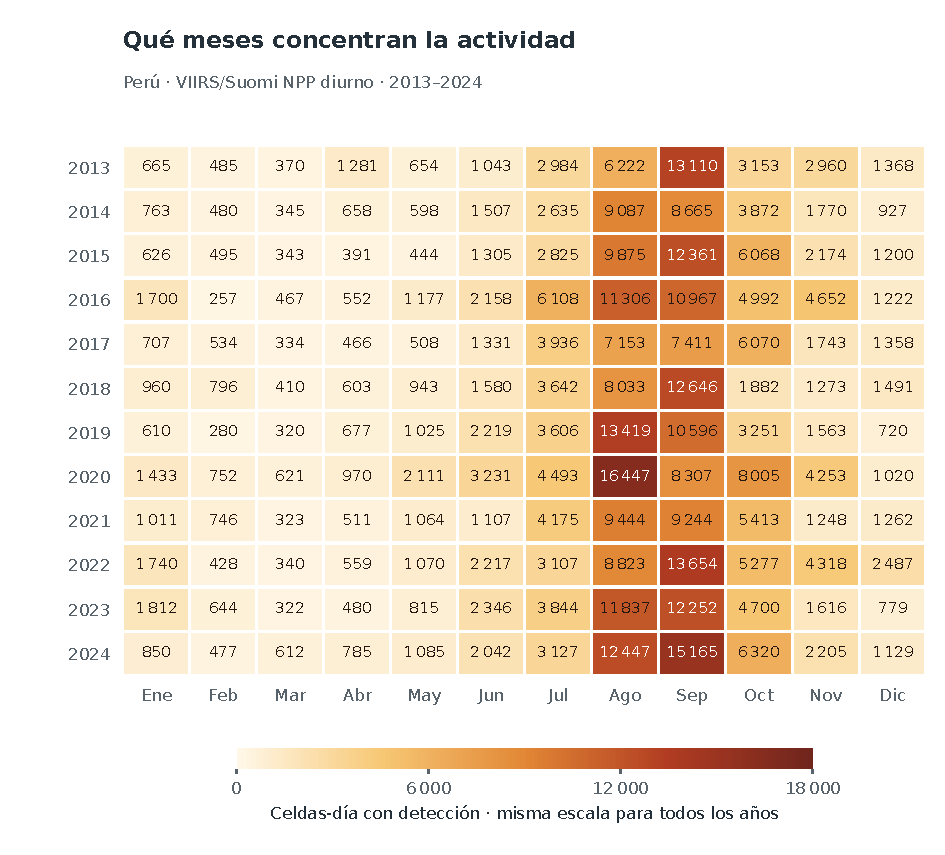
\includegraphics[width=\textwidth]{figuras/peru_calendario.pdf}
\caption{\textbf{Datos reales de Perú, 2013--2024.} Actividad diurna registrada por VIIRS/Suomi
NPP, tipo 0 y confianza nominal/alta, agrupada en celdas de $0{,}05^\circ$ y día local.
No se suman NOAA-20 ni NOAA-21. Fuente: CSV nacionales de NASA FIRMS; cálculo propio
reproducible en \texttt{scripts/analizar\_peru.py}. Sin corrección de cobertura ni nubes.}
\label{fig:peru-calendario}
\end{figure}

Primero se lee verticalmente: ¿el mismo mes tiende a ser activo en muchos años? Eso sugiere
un componente estacional. Luego se lee horizontalmente: ¿un año concentra su actividad en
pocos meses o la distribuye más? Finalmente se comparan filas: ¿hay un año distinto? Cada
pregunta es diferente. Un color intenso en septiembre no demuestra por sí solo una anomalía:
septiembre puede ser habitualmente intenso.

Hay un límite espacial importante. Perú contiene costa, sierra y selva, con climas y usos
del suelo distintos. Una curva nacional puede mezclar temporadas regionales diferentes.
Sirve para aprender el procedimiento y describir el conjunto; no debe convertirse en una
fecha única de preparación para cada municipio. Para Junín se necesitaría recortar las
detecciones con un límite administrativo documentado y repetir \emph{todo} el cálculo.
Un rectángulo alrededor de Huancayo no equivale al departamento de Junín.

\FloatBarrier
\section{Qué significa lo habitual}

\begin{definicion}{referencia estacional}
Una referencia estacional es la distribución histórica de una misma variable, en una misma
región y una misma posición del calendario, calculada con un periodo de referencia declarado.
Comparar un septiembre con otros septiembres controla la parte más evidente de la estacionalidad.
\end{definicion}

La referencia de este caso son los once años 2013--2023. Reservamos 2024 para compararlo.
Para cada mes calculamos la mediana y los percentiles 10 y 90 de sus once valores. Usamos
interpolación lineal: si los valores ordenados son $x_{(1)},\ldots,x_{(n)}$, la posición
del percentil $p$ es $h=1+(n-1)p$, con $p$ entre cero y uno. Se interpola entre las dos
posiciones vecinas. Con once años, $p=0{,}9$ da $h=10$: el percentil 90 es el décimo valor
ordenado. Explicitar la convención evita diferencias entre programas.

\begin{figure}[!htbp]
\centering
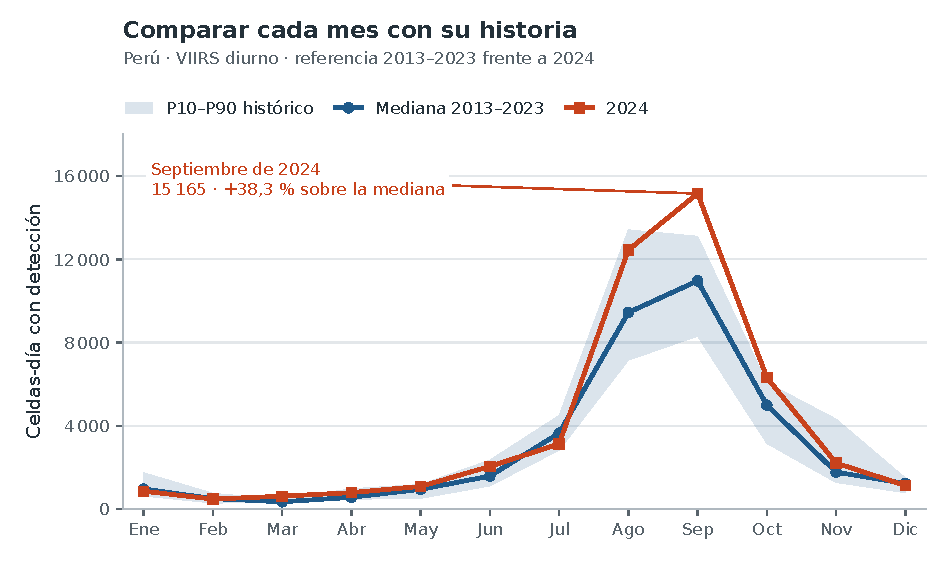
\includegraphics[width=\textwidth]{figuras/peru_perfil.pdf}
\caption{El mismo registro real de Perú, comparado por mes. La banda es variabilidad histórica
entre años; \textbf{no} es un intervalo de confianza de la mediana ni un pronóstico. Todos los
valores usan la selección de la tabla~\ref{tab:contrato-peru}.}
\label{fig:peru-perfil}
\end{figure}

Una referencia fija facilita comparar versiones de la aplicación: <<respecto de 2013--2023>>
siempre quiere decir lo mismo. Una referencia móvil se adapta a cambios recientes, pero
también cambia la vara de medir. Si cada año se actualiza, deben conservarse su versión y
los años que la integran. No existe una elección universalmente correcta; la elección
depende de si se quiere describir una anomalía respecto de un pasado fijo o del pasado reciente.

\begin{atencion}[Once años no son once certezas]
Los años pueden estar relacionados entre sí y el sistema de observación puede cambiar.
Una mediana robusta frente a un valor extremo no corrige esas dependencias ni elimina una
tendencia. Además, la serie nacional de once años no es una normal climatológica de treinta
años. En el libro la llamamos referencia histórica, indicando su duración.
\end{atencion}

\FloatBarrier
\section{Anomalía no significa automáticamente emergencia}

Si $b_m$ es la mediana de referencia y $C_m$ la actividad que comparamos, definimos
\begin{align}
 \Delta_m &= C_m-b_m,\label{eq:anom-absoluta}\\
 a_m &=100\left(\frac{C_m}{b_m}-1\right),\qquad b_m>0.\label{eq:anom-relativa}
\end{align}
La primera mide cuántas celdas-día adicionales aparecen en el registro; la segunda, la
diferencia relativa en porcentaje. Ambas tienen utilidad. Pasar de 1 a 4 produce una
anomalía del 300\,{}\%, pero una diferencia absoluta de solo tres unidades. Pasar de 4000 a
6000 produce un 50\,{}\% y dos mil unidades adicionales. El porcentaje por sí solo no
ordena la magnitud operativa del problema.

\begin{ejemplo}{septiembre de 2024 en Perú}
Con nuestra selección de datos, septiembre de 2024 contiene \PeruSeptActual{} celdas-día.
La mediana de septiembre de 2013--2023 es \PeruSeptMediana{} y su percentil 90 es
\PeruSeptQnoventa{}. ¿Cómo se expresa la diferencia?
\solucion Aplicando la ecuación~\eqref{eq:anom-relativa}, la diferencia respecto de la
mediana es \PeruSeptAnomalia{} por ciento. Esta cifra se refiere a actividad \emph{detectada}
por un sensor, con una rejilla y unos filtros concretos. No es el porcentaje de superficie
quemada ni el aumento del número de incendios reportados por las autoridades. Puede
reproducirse consultando la fila de septiembre en \texttt{datos/peru\_climatologia.csv}.
\end{ejemplo}

Si $b_m=0$, la razón no existe. No añadimos uno de forma silenciosa: cambiaría el significado
del indicador. Se puede informar <<hay detecciones; la mediana de referencia es cero>>,
mostrar la diferencia absoluta y ampliar la ventana temporal. Cuando el valor de referencia
es muy pequeño, incluso una razón definida es inestable. Un umbral mínimo para mostrar
porcentajes debe justificarse y mantenerse fijo.

Otra forma de describir una observación es su posición respecto de los años históricos.
Si supera a los once septiembres de referencia, es mayor que todos los valores de esa
muestra. No significa que su periodo de retorno sea infinito, ni que tenga probabilidad
uno de causar daños. Una muestra corta informa poco sobre los extremos.

\subsection{Desviación estándar y medidas robustas}

Con media $\bar C_m$ y desviación muestral $s_m$, el puntaje
\begin{equation}
 z_m=\frac{C_m-\bar C_m}{s_m}
\end{equation}
expresa cuántas desviaciones separan el valor de la media. Es una escala, no una prueba
automática de significación. Convertir $z=2$ en una probabilidad exige un modelo de
distribución que un conteo de fuegos asimétrico quizá no cumpla.

Una alternativa usa la mediana y la desviación absoluta mediana,
\begin{equation}
 \operatorname{MAD}=\operatorname{mediana}_y|C_{y,m}-b_m|,
 \qquad z_m^{\mathrm{rob}}=\frac{C_m-b_m}{1{,}4826\operatorname{MAD}}.
\end{equation}
El factor 1,4826 hace comparable la escala con una desviación estándar bajo normalidad;
no vuelve normales los datos. Si MAD es cero, el puntaje no se calcula. Para un público
general, mediana, rango histórico y diferencia absoluta suelen explicar más que una sigla.
La identificación de valores atípicos debe distinguir una señal interesante de un error
de medición o de un modelo inadecuado.\fuente{nist}

\FloatBarrier
\section{Cuándo empieza la temporada}

La pregunta tiene varias respuestas posibles. El primer foco del año depende mucho de
una detección aislada. El mes de máximo conteo es inestable si hay dos picos parecidos.
Una alternativa más gradual usa la fracción acumulada de actividad anual.

Para un año con actividad total positiva, definimos
\begin{equation}\label{eq:fraccion-estacional}
 p_{y,m}=\frac{C_{y,m}}{\sum_{j=1}^{12}C_{y,j}},\qquad
 \bar p_m=\frac{1}{n}\sum_y p_{y,m},\qquad
 F_m=\sum_{j=1}^{m}\bar p_j.
\end{equation}
Normalizar cada año antes de promediar da el mismo peso a todos los años válidos. En cambio,
dividir la suma de todos los agostos entre la suma de todos los años da más peso a los años
de gran actividad. Son preguntas distintas: una describe un año típico en forma, la otra
distribuye todas las unidades registradas durante el periodo.

\begin{figure}[!htbp]
\centering
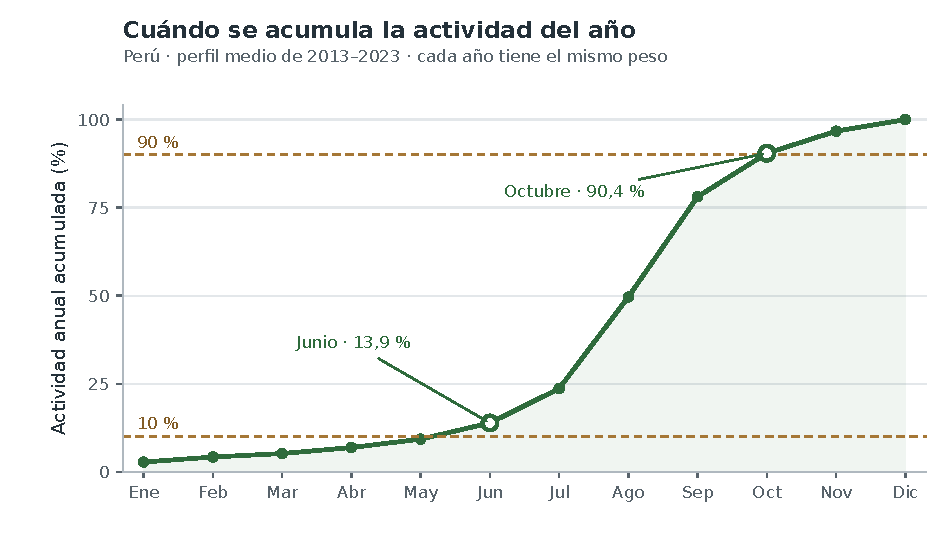
\includegraphics[width=\textwidth]{figuras/peru_acumulado.pdf}
\caption{Fracción acumulada media del año para Perú, VIIRS diurno, 2013--2023. Cada año se
normaliza por su propio total antes del promedio. Las líneas del 10 y el 90\,{}\% ilustran
una definición de ventana central de actividad, no umbrales oficiales de alerta.}
\label{fig:peru-acumulado}
\end{figure}

Podemos llamar comienzo de la ventana central al primer mes que alcanza el 10\,{}\% y
final al que alcanza el 90\,{}\%. Esa ventana contiene aproximadamente el 80\,{}\% central
de la actividad de la distribución estacional. Con datos mensuales la resolución es mensual:
dar un día exacto mediante interpolación supondría que la actividad se reparte uniformemente
dentro del mes. Si se necesita una fecha, se repite el cálculo con días o semanas y se
explica el suavizado.

\begin{ejemplo}{una cifra estacional reproducible}
En el perfil peruano de 2013--2023, la suma de las fracciones medias de agosto, septiembre
y octubre es \PeruASO{} por ciento. ¿Significa que cada año tuvo exactamente esa fracción?
\solucion No. Se normalizó cada año y se promediaron sus fracciones. Un año puede anticipar
o retrasar la temporada. La cifra resume la concentración media de la actividad detectada
en esos tres meses; su variabilidad se estudia conservando las fracciones de cada año.
\end{ejemplo}

En una zona con dos temporadas separadas, una sola ventana 10--90 puede incluir un periodo
intermedio poco activo. En una zona cuya temporada cruza diciembre hay que elegir un año
de actividad, por ejemplo julio a junio, y conservarlo. El calendario debe seguir al
fenómeno, no imponerle por comodidad la forma del año civil.

\FloatBarrier
\section{Meses incompletos y suavizado}

El 12 de septiembre todavía no existe el total de septiembre. Comparar sus primeros doce
días con meses completos produce una falsa caída. Hay dos comparaciones honestas: esperar
a cerrar el mes o comparar del 1 al 12 con del 1 al 12 de cada año histórico. En el segundo
caso deben utilizarse también archivos con una madurez semejante, o marcar que lo reciente
es provisional y puede revisarse.

Multiplicar un conteo parcial por $30/12$ es una proyección que supone un ritmo uniforme.
Puede servir como escenario simple, pero falla si la temporada está creciendo o si faltó
una pasada decisiva. No se etiqueta como total observado.

Para visualizar una serie diaria se puede suavizar con una media móvil. Una media centrada
de siete días en $d$ usa desde $d-3$ hasta $d+3$; una media retrospectiva usa desde $d-6$
hasta $d$. La centrada es útil para una figura histórica, pero conoce tres días del futuro.
No debe utilizarse sin cambios para evaluar una señal emitida en el día $d$.
Los métodos de evaluación temporal hacen explícita esta frontera entre pasado disponible
y futuro reservado.\fuente{forecast}

\FloatBarrier
\section{Qué incertidumbre dibujar}

Hay al menos tres bandas diferentes que podrían rodear una curva. La banda P10--P90 de la
figura~\ref{fig:peru-perfil} describe cómo variaron años pasados. Un intervalo de confianza
de la mediana describe la incertidumbre de estimar esa mediana con pocos años. Un intervalo
de predicción intenta cubrir una observación futura. Las tres bandas responden preguntas
distintas y no deben compartir una leyenda genérica de <<error>>.

En una serie armonizada aparece otra incertidumbre: la de la calibración. Si muchas
celdas usan la misma razón $r$, sus errores de conversión están relacionados. No se debe
sortear una razón independiente para cada celda: al sumar miles de celdas, esa simulación
haría desaparecer artificialmente la incertidumbre común.

Un procedimiento más fiel remuestrea bloques de años del periodo de ajuste, vuelve a
estimar una razón por estrato y aplica esa misma razón a todas las celdas del estrato en
cada réplica. Después construye el calendario de esa réplica. La dispersión final transmite
la incertidumbre estimada del ajuste. Sigue sin reconstruir fuegos ocultos ni corregir
sesgos desconocidos; su alcance debe escribirse junto a la banda.

\FloatBarrier
\section{De la anomalía a una decisión}

Una aplicación puede señalar <<actividad registrada por encima del P90 histórico>> y
proponer revisar las observaciones. Para llamarlo alerta predictiva tendría que demostrar
que una señal emitida con información disponible hasta hoy anticipa un resultado futuro
definido. Harían falta una ventana de anticipación, una variable objetivo, datos de
verificación y evaluación fuera de muestra. El calendario histórico es una pieza útil
para prepararse; por sí solo no predice dónde arderá mañana.

Además, al revisar muchos lugares aparecen valores extremos por casualidad. Si cincuenta
series independientes tienen cada una una probabilidad de 0,1 de superar cierto umbral
en un periodo, se esperan cinco superaciones, y la probabilidad de al menos una es
$1-0{,}9^{50}\approx99{,}5\,{}\%$. En la realidad hay dependencia espacial y umbrales
estimados, de modo que ese cálculo es solo una ilustración. Enseña por qué <<algo salió
rojo en el mapa>> no demuestra una emergencia.\fuente{isl}

Para evaluar señales operativas se necesita revisar persistencia, magnitud absoluta,
calidad de observación y un resultado independiente de los mismos datos usados para
crear la señal. Un percentil es un descriptor; una decisión también incorpora consecuencias
y conocimiento del territorio.

\resumen
\begin{itemize}
\item Una casilla puede contar detecciones, celdas-día o un índice equivalente. La unidad
debe conservarse desde el archivo hasta la pantalla.
\item Cero detecciones, celda no observable y archivo ausente son estados distintos.
\item La referencia compara el mismo mes, región, selección y unidad; se declara su periodo.
\item Una anomalía se acompaña de magnitud absoluta, referencia e información de cobertura.
\item El calendario real de Perú se reproduce desde los CSV de FIRMS y no constituye un
censo de incendios ni una estimación de área quemada.
\item Una temporada definida mediante acumulados es retrospectiva; no anticipa por sí sola
los incendios del año siguiente.
\end{itemize}

\ejercicios
\begin{enumerate}
\item A partir de \path{datos/peru_mensual.csv}, comprueba el total anual de VIIRS de 2024 por
dos caminos: sumando meses y contando las claves de celda-día del archivo original.
\item En una cuadrícula de 40 celdas, ¿cuál es el máximo de celdas-día de febrero de 2024?
¿Qué interpretación tendría una conversión que superara ese máximo?
\item Calcula para agosto la anomalía de 2024 respecto de la mediana 2013--2023 y contrástala
con la cifra \PeruAgostoAnomalia{} por ciento. Explica el efecto de usar una media.
\item Ordena los once septiembres de referencia y comprueba su percentil 90 con la convención
del texto. ¿Cuánto cambia si se excluye un solo año extremo?
\item Repite el perfil estacional dando a cada celda-día el mismo peso en todo el periodo,
en vez de dar el mismo peso a cada año. Explica por qué las curvas no tienen que coincidir.
\item Una API devuelve cero filas para un día. Enumera tres explicaciones distintas y qué
metadatos permitirían distinguirlas.
\item Diseña la comparación que mostrarías el 12 de septiembre. Indica exactamente qué
fechas usarías en cada año de referencia y qué dato futuro queda excluido.
\item Una mediana es cero y el valor actual es cinco. Redacta una frase informativa sin
inventar un porcentaje ni llamarlo incendio confirmado.
\item Describe cómo remuestrearías la incertidumbre de un calendario cuyas 2000 celdas
comparten una sola razón de calibración. ¿Por qué no sortear 2000 razones independientes?
\item Propón un criterio comprobable para afirmar que una herramienta anticipa actividad
con una semana de antelación. Separa variable objetivo, datos disponibles y periodo de prueba.
\end{enumerate}

\lecturas
La investigación de Giglio, Csiszar y Justice sobre distribución y estacionalidad del fuego
activo sitúa el calendario en su contexto científico.\fuente{giglio-season} Para evaluar
series sin introducir información futura, consulta el capítulo sobre herramientas de
pronóstico de Hyndman y Athanasopoulos.\fuente{forecast} El archivo de FIRMS y el programa
del caso peruano permiten practicar cada paso con datos reales, en lugar de memorizar
una curva estacional.\fuente{firms-country}


\part{Hacia la aplicación}
\chapter{Hacia una aplicación rápida, explicable y reproducible}\label{cap:aplicacion}

\objetivos{\begin{itemize}
\item Traducir las definiciones científicas en un modelo de datos sin perder su significado.
\item Separar el procesamiento histórico de las consultas interactivas.
\item Explicar el papel de las columnas, la memoria, la caché y el paralelismo.
\item Evaluar una calibración con datos reales de Perú reservados para prueba.
\item Diseñar una interfaz que muestre tanto el resultado como la evidencia que lo sostiene.
\end{itemize}}

\FloatBarrier
\section{La aplicación comienza antes de la pantalla}

Un mapa que se mueve con fluidez puede estar contando mal. Una ecuación correcta puede ser
inutilizable si obliga a esperar minutos cada vez que se cambia de provincia. Construir
una herramienta útil exige unir dos responsabilidades: preservar el significado de los
datos y dar respuesta dentro del tiempo que necesita el usuario.

El punto de partida es escribir una pregunta precisa. Por ejemplo: <<Para un área elegida,
mostrar la actividad de fuego detectada por mes, comparada con una referencia histórica,
y permitir inspeccionar cómo cambia al armonizar los sensores>>. Esa frase ya determina
qué debe guardar el programa y qué necesita calcular al recibir una consulta. No exige
que el navegador lea cada detección original.

Antes de elegir una biblioteca, fija seis cosas: área cubierta, años cubiertos, unidad,
plataformas, filtros y significado del cero. La tabla~\ref{tab:contrato-peru} es un ejemplo
de ese contrato. Si la base de datos almacena celdas-día y la interfaz rotula el resultado
como <<incendios>>, ninguna optimización posterior puede reparar la interpretación.

\FloatBarrier
\section{Tres capas con responsabilidades distintas}

Conviene separar los archivos originales, las tablas normalizadas y los productos de
consulta. La separación no es burocrática: permite volver a una etapa anterior cuando
se descubre un error o cambia una definición.

\begin{figure}[ht]
\centering
\begin{tikzpicture}[node distance=8mm]
\node[caja,fill=cenizaClaro,text width=3.7cm] (a) {\textbf{Originales}\\CSV de FIRMS\\URL, fecha, huella};
\node[caja,fill=cieloClaro,text width=3.7cm,right=of a] (b) {\textbf{Observaciones}\\esquema común\\sensor y versión};
\node[caja,fill=bosqueClaro,text width=3.7cm,right=of b] (c) {\textbf{Indicadores}\\celdas-día, calendario\\modelo y referencia};
\draw[flujo] (a)--(b);\draw[flujo] (b)--(c);
\node[caja,below=10mm of c,text width=3.7cm,fill=brasaClaro] (d) {\textbf{Consulta y pantalla}\\área, periodo, comparación};
\draw[flujo] (c)--(d);
\node[align=left,font=\small,text width=8cm,anchor=west] at (-1.8,-2) {Un cambio de filtro invalida los indicadores.\\Un cambio de color no obliga a descargar datos otra vez.};
\end{tikzpicture}
\caption{Arquitectura conceptual del procesamiento. Las flechas representan transformaciones
reproducibles, no pasos que deban repetirse en cada interacción.}
\label{fig:arquitectura}
\end{figure}

Los \textbf{originales} se conservan sin corregir. Un manifiesto identifica cada archivo con
su fuente, fecha de adquisición, tamaño y huella criptográfica. La huella detecta un cambio
de contenido; no certifica que la medición sea verdadera. Guardar la versión del algoritmo
es tan necesario como guardar el sensor.

La \textbf{tabla normalizada} conserva una fila por detección y tipos de datos explícitos:
coordenadas numéricas, fecha UTC, identificador de plataforma, clase de confianza, FRP,
tipo y procedencia. La clase de confianza original no se convierte en una supuesta
probabilidad común. Un valor desconocido se representa como desconocido, no como cero.
El tutorial de FIRMS sobre ingestión muestra los problemas prácticos de fechas y columnas
que conviene resolver en esta fase.\fuente{firms-ingest}

La \textbf{tabla de indicadores} contiene claves únicas y sus atributos. Una clave para
el caso del libro es (plataforma, celda, fecha local), porque se seleccionaron solo
pasadas diurnas. En una aplicación que conserve día y noche separados, la franja forma
parte de la clave. La tabla mensual se obtiene de esas claves, no directamente de una
suma de focos.

\begin{ejemplo}{una clave omitida cambia el resultado}
En una misma celda y día, Aqua registra dos focos y Suomi NPP cinco. Si se agrupa únicamente
por celda y fecha, queda una fila. ¿Por qué es incorrecto para calibrar?
\solucion Se perdió qué plataforma observó cada presencia. Para comparar sensores hacen
falta dos indicadores separados, uno por plataforma. La unión podría ser útil como
producto de vigilancia con múltiples satélites, pero ya no tiene la misma probabilidad
de detección que una serie histórica basada en uno solo.
\end{ejemplo}

\FloatBarrier
\section{Operaciones que parecen equivalentes y no lo son}

Algunas agregaciones son sumables; otras requieren conservar conjuntos. Si dos meses
contienen días distintos, sus conteos de celdas-día pueden sumarse. Si dos satélites
registran la misma celda el mismo día, sus presencias no pueden sumarse para obtener
la presencia conjunta. Hay que tomar la unión.

También cambia la respuesta al cambiar el tamaño de celda. Supón cuatro celdas pequeñas
que forman una grande y presentan fuego el mismo día. La actividad sobre la rejilla fina
es cuatro celdas-día. La presencia en la celda grande es una. Sumar las cuatro conserva
la unidad fina; deduplicar después de cambiar de rejilla construye otra unidad. Ambas
operaciones son posibles, pero no se rotulan igual.

\begin{figure}[ht]
\centering
\begin{tikzpicture}[x=1cm,y=1cm]
\foreach \x/\y in {0/0,0/1,1/0,1/1}{\fill[brasaClaro] (\x,\y) rectangle ++(1,1);\fill[fuego] (\x+.5,\y+.5) circle(.08);}
\draw[step=1] (0,0) grid (2,2);
\node[align=center,font=\small] at (1,-.6) {4 celdas-día\\en rejilla fina};
\draw[flujo] (2.5,1)--(4,1) node[midway,above,font=\small]{sumar};
\node[caja,fill=cieloClaro,text width=2.8cm] at (5.7,1) {4 unidades finas\\en un área mayor};
\draw[flujo] (2.5,0)--(2.5,-1.5)--(4,-1.5);
\node[font=\small,align=center,anchor=north] at (3.25,-1.75) {reagrupar\\y unir};
\node[caja,fill=bosqueClaro,text width=2.8cm] at (5.7,-1.5) {1 celda-día\\en rejilla gruesa};
\node[align=left,font=\small,text width=4cm] at (10.5,0) {La geometría del área es la misma.\\La unidad estadística ha cambiado.};
\end{tikzpicture}
\caption{Dos preguntas diferentes sobre las mismas detecciones. Esquema didáctico. Una pirámide
de mapas debe documentar cuál de estas operaciones representa cada nivel.}
\label{fig:agregacion}
\end{figure}

Los bordes administrativos añaden otra decisión. Asignar una celda a una provincia por
su centro es rápido, pero aproximado. Repartir una celda según su fracción de área dentro
de cada provincia produce unidades ponderadas, no localiza el fuego dentro de la celda.
Si se necesita un conteo preciso por polígono, se recortan las detecciones originales
antes de agrupar, con una regla consistente para los puntos en el borde. La resolución
debe responder a la pregunta y a la precisión de geolocalización disponible.

\FloatBarrier
\section{Por qué los archivos columnares ayudan}

Un CSV es excelente para inspección y distribución, pero todas sus cifras son texto.
Cada lectura debe encontrar separadores, interpretar cadenas y reconstruir tipos. En
una consulta que solo necesita fecha, celda y plataforma, leer también temperaturas y
otras columnas consume ancho de banda y tiempo sin aportar información.

Un formato columnar agrupa los valores de cada columna. Así, las consultas pueden
leer solo las columnas necesarias y comprimir secuencias de valores parecidos. Parquet
es un formato abierto que organiza los datos de ese modo.\fuente{parquet} No es una
base de datos ni acelera por sí solo cualquier tarea: el resultado depende de la
organización de archivos, el motor de lectura y los filtros.

\begin{ejemplo}{un presupuesto de memoria}
Supón diez millones de filas con fecha como entero de 64 bits; celda, latitud y longitud
como valores de 32 bits; plataforma y clase como enteros de 8 bits. ¿Cuánto ocupan los
valores sin índices ni estructuras auxiliares?
\solucion Cada fila aporta $8+4+4+4+1+1=22$ bytes. El total es 220 millones de bytes,
aproximadamente 210 MiB. Una lista de diccionarios de Python añade objetos, referencias
y tablas hash, y puede ocupar mucho más. El cálculo es un presupuesto teórico, no una
medición de una biblioteca concreta. Para verificarlo se mide la memoria del proceso.
\end{ejemplo}

El vínculo con arquitectura de computadoras es directo. Leer columnas contiguas favorece
la localidad espacial: cuando una línea de caché trae varios valores próximos, muchos
serán útiles enseguida. Saltar entre millones de objetos dispersos reduce ese beneficio.
Una operación vectorizada también evita ejecutar un bucle interpretado por cada fila,
aunque sigue limitada por el movimiento de memoria cuando la aritmética es simple.

Particionar por año y plataforma permite descartar archivos enteros antes de leerlos.
Dentro del archivo, ciertas estadísticas permiten descartar grupos de filas. DuckDB
documenta la lectura selectiva de columnas y el traslado de filtros al lector de
Parquet; esas optimizaciones dependen de la organización y las estadísticas del archivo.
\fuente{duckdb} Particionar por cada celda minúscula puede producir tantos archivos
pequeños que el coste de abrirlos supere el trabajo útil.

\FloatBarrier
\section{Dos estrategias para construir las celdas-día}

Con $N$ detecciones, una tabla hash de claves únicas suele construir las presencias
en tiempo esperado $O(N)$. Su memoria depende del número de claves distintas y de la
representación. Ordenar por plataforma, celda y fecha requiere generalmente
$O(N\log N)$ comparaciones, pero luego basta recorrer los registros contiguos y
emitir una fila cuando cambia la clave.

La estrategia de ordenación puede funcionar con datos mayores que la memoria: se
ordenan fragmentos y después se mezclan. La de hash necesita particionar o volcar a
disco si sus claves no caben. El punto no es declarar ganadora una complejidad; es
medir con tamaños y límites de memoria representativos.

\begin{lstlisting}[caption={Pseudocódigo: presencia diaria por plataforma.}]
para cada archivo:
    verificar esquema y version
    para cada fila aceptada:
        fecha_local = convertir_fecha_hora_utc(fila)
        celda = asignar_rejilla(fila.latitud, fila.longitud)
        guardar_clave_unica(plataforma, celda, fecha_local)

para cada clave unica:
    mensual[plataforma, anio, mes] += 1
\end{lstlisting}

El ejemplo reproducible del libro usa Python estándar y conjuntos, para que se pueda
leer sin instalar un motor analítico. Es una implementación de referencia, no una
afirmación de rendimiento óptimo. Una implementación más rápida debe producir
exactamente las mismas claves bajo el mismo contrato antes de compararse en velocidad.

\FloatBarrier
\section{Qué precalcular y qué responder en vivo}

La descarga, normalización, revisión de versiones y construcción de claves se hacen
cuando cambia el conjunto de datos. La estimación de razones y la referencia estacional
cambian con menor frecuencia. La selección de un área y el dibujo de su calendario
deben reutilizar esos resultados.

Una consulta puede recibir una lista de celdas y sumar sus indicadores mensuales.
Pero si la calibración es no lineal, o depende de estratos, el orden importa:
$f(x_1+x_2)$ no suele ser igual a $f(x_1)+f(x_2)$. Incluso con una razón lineal, dos
estratos con razones distintas requieren $r_1x_1+r_2x_2$, no una razón elegida a posteriori
para el total. El modelo tiene una escala de validez y la interfaz debe respetarla.

Una caché guarda respuestas ya calculadas. Su clave debe incluir área, periodo, rejilla,
plataformas, filtros, versión de datos, modelo y referencia histórica. Si solo usa
<<Perú, septiembre>>, devolverá cifras viejas después de actualizar la calibración.
Invalidar correctamente la caché es parte de la corrección científica.

En el navegador conviene enviar celdas agregadas, curvas y metadatos; los puntos originales
se solicitan cuando el usuario inspecciona una zona pequeña. Un archivo de un millón de
coordenadas tarda en transferirse, analizarse y dibujarse aunque el servidor haya calculado
la suma en milisegundos. Se mide el tiempo hasta que el usuario ve una respuesta útil.

\FloatBarrier
\section{Paralelismo con una medida de sus límites}

Los archivos de años distintos pueden procesarse de forma independiente y después
combinarse, si las reglas para fechas en los bordes están controladas. Los estratos de
calibración también admiten trabajo independiente. Eso no significa que cada etapa
mejore linealmente al añadir núcleos.

Si una fracción $p$ del tiempo puede paralelizarse idealmente y el resto es serial,
la aceleración con $k$ trabajadores está limitada por
\begin{equation}\label{eq:amdahl}
 S(k)=\frac{1}{(1-p)+p/k}.
\end{equation}
Es la ley de Amdahl bajo sus supuestos: tamaño de problema fijo, parte paralela ideal
y sin costes extra de coordinación.\fuente{amdahl}

\begin{ejemplo}{ocho núcleos no dan ocho veces más velocidad}
Una versión tarda 100 segundos, de los cuales 80 pueden repartirse. ¿Cuánto tardaría
idealmente con ocho trabajadores?
\solucion La parte serial conserva 20 segundos y la paralela baja a $80/8=10$.
El total es 30 segundos, una aceleración de $100/30\approx3{,}33$. Con infinitos
trabajadores el límite sería cinco veces. Si el disco o la memoria ya están saturados,
la mejora real será menor. Antes de paralelizar se identifica dónde se va el tiempo.
\end{ejemplo}

Para este problema suele rendir más evitar lecturas repetidas y objetos innecesarios
que empezar por una GPU. Una GPU puede ser útil en operaciones grandes y regulares,
pero transferir datos y preparar estructuras tiene un coste. La elección se hace
después de medir, sin cambiar la definición del indicador para mejorar un benchmark.

\FloatBarrier
\section{Laboratorio real: una calibración para Perú}\label{sec:peru-validacion}

Ahora ponemos a prueba una de las recetas del capítulo~\ref{cap:armonizacion}. Elegimos
2018--2022 porque sus archivos MODIS comparten la etiqueta \texttt{6.03}; VIIRS conserva
\texttt{2}. Se ajusta una razón con 2018--2020 y se reservan 2021--2022 para probarla.
No se eligen los años por el tamaño del error. Es una demostración nacional con tres
años de ajuste y dos de prueba, no una validación suficiente para cualquier región.

Los filtros y la rejilla son los de la tabla~\ref{tab:contrato-peru}. En los años de
ajuste se registran \PeruAjusteAqua{} celdas-día de Aqua y \PeruAjusteVIIRS{} de Suomi NPP.
La razón de sumas es
\begin{equation}
 \widehat r=\frac{124188}{26508}\approx4{,}685.
\end{equation}
Esto no significa que cada fuego de Aqua se divida en 4,685 incendios de VIIRS. Es la
relación agregada entre dos indicadores de detección, bajo esta selección y durante
este periodo. Incluye diferencias de sensibilidad, cobertura y oportunidad de observación.

\begin{table}[ht]
\centering
\begin{tabular}{lrrl}
\toprule
Año & Aqua: celdas-día & Suomi NPP: celdas-día & Uso \\
\midrule
2018 & \num{7569} & \num{34259} & Ajuste \\
2019 & \num{9491} & \num{38286} & Ajuste \\
2020 & \num{9448} & \num{51643} & Ajuste \\
2021 & \num{7344} & \num{35548} & Prueba \\
2022 & \num{10231} & \num{44020} & Prueba \\
\bottomrule
\end{tabular}
\caption{Valores reales de Perú. Cada total resulta de sumar los doce meses de la misma
plataforma; los filtros se mantienen constantes. Los años de prueba no entran en la razón.}
\label{tab:peru-ajuste}
\end{table}

Aplicamos $\widehat V_m=\widehat r A_m$ a cada mes de prueba y comparamos con el VIIRS
observado de ese mes. La comparación es entre sensores; VIIRS también tiene errores y
no es una verdad de terreno perfecta.

\begin{figure}[!htbp]
\centering
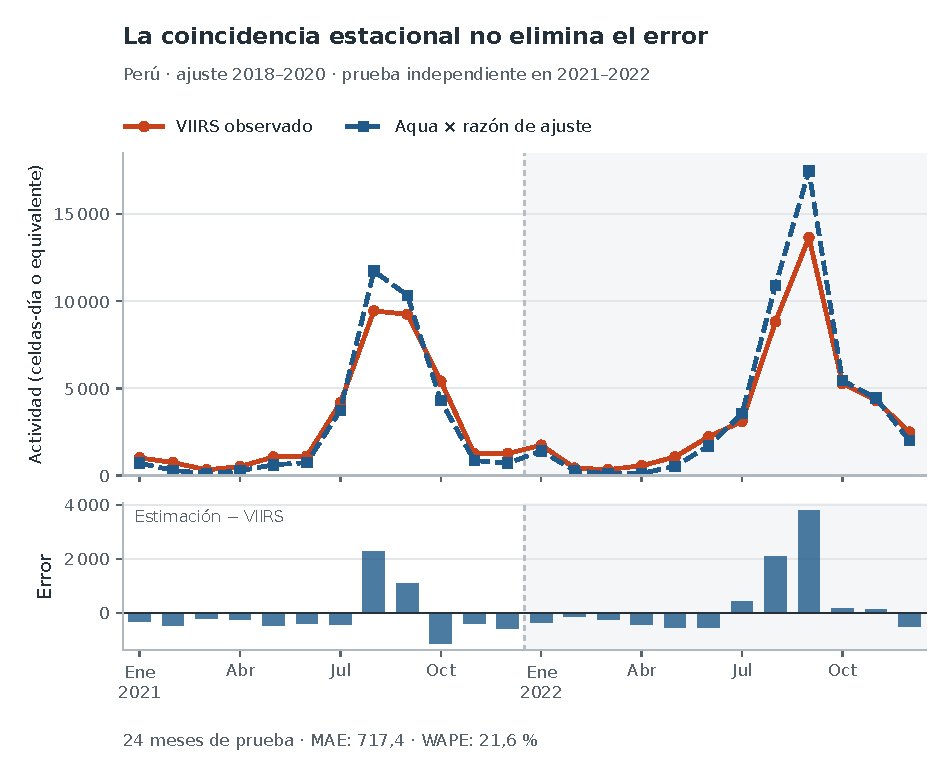
\includegraphics[width=\textwidth]{figuras/peru_validacion.pdf}
\caption{Validación temporal real en Perú. La razón se ajustó con 2018--2020 y se aplicó
sin cambios a los 24 meses de 2021--2022. Una buena coincidencia del ciclo estacional
no garantiza que coincidan las amplitudes mensuales. El panel inferior muestra el error
firmado: por encima de cero la conversión sobreestima el registro VIIRS; por debajo,
lo subestima.}
\label{fig:peru-validacion}
\end{figure}

El MAE de prueba es \PeruMAE{} unidades mensuales y el sesgo medio es
$+\PeruSesgo{}$. Para expresar un error relativo sin dividir cada mes por su propio
conteo, usamos
\begin{equation}\label{eq:wape}
 \mathrm{WAPE}=100\frac{\sum_m|\widehat V_m-V_m|}{\sum_m V_m},\qquad \sum_m V_m>0.
\end{equation}
Resulta \PeruWAPE{} por ciento. Esta medida da más influencia a los meses de gran
actividad. No afirma que cada mes tenga ese porcentaje de error; se acompaña del
gráfico de residuos y del MAE. Si todos los valores observados son cero, tampoco WAPE
está definido.

\begin{atencion}[El resultado real no se maquilla]
La razón única captura parte de la relación, pero deja desacuerdos apreciables. No
ajustamos el factor con los años de prueba para que las curvas queden bonitas. Un paso
posterior podría estudiar estratos regionales o estacionales, cobertura y estabilidad
temporal. Habría que seleccionar esas variantes con validación interna y evaluarlas en
otros años reservados. Este resultado es una línea base reproducible.
\end{atencion}

La diferencia entre los dos totales anuales puede ser pequeña por cancelación de
errores mensuales. Sobreestimar agosto y subestimar septiembre puede dejar un año casi
perfecto mientras arruina el calendario operativo. Por eso se evalúa en la resolución
temporal para la que se quiere usar el producto.

\FloatBarrier
\section{Segundo experimento: la razón no es constante}\label{sec:peru-modelos}

El panel de errores de la figura~\ref{fig:peru-validacion} no es ruido: la conversión
sobreestima los meses de más actividad y subestima los de menos, los dos años. Un error
con forma indica que al modelo le falta algo. El capítulo~\ref{cap:deteccion} anticipa
qué: fuera de temporada predominan fuegos pequeños, que Aqua casi no registra, y la razón
entre sensores debería ser mayor.

Para comprobarlo se calcula la razón de sumas de cada mes del año con los tres años de
ajuste (figura~\ref{fig:peru-razon-mensual}). Va de \PeruRazonMin{} en septiembre a
\PeruRazonMax{} en marzo: cambia más de tres veces a lo largo del año. La razón única de
\PeruRatio{} es, en la práctica, la razón de agosto y septiembre, porque esos dos meses
aportan dos tercios de las celdas-día de Aqua.

\begin{figure}[!htbp]
\centering
\begin{tikzpicture}
\begin{axis}[width=13cm,height=6.2cm,ybar,bar width=14pt,ymin=0,ymax=13,
  xmin=0.3,xmax=12.7,xtick={1,...,12},xticklabels={E,F,M,A,M,J,J,A,S,O,N,D},
  ylabel={Razón Suomi NPP / Aqua},axis lines*=left,ymajorgrids,grid style={ceniza!20},
  nodes near coords,nodes near coords style={font=\scriptsize,/pgf/number format/.cd,fixed,precision=1,use comma},
  ]
\addplot[fill=fuego!70,draw=none] table[x=mes,y=razon]{datos/peru_razon_mensual.dat};
\draw[cielo,very thick,dashed] (axis cs:0.3,4.685)--(axis cs:12.7,4.685);
\node[cielo,font=\footnotesize,anchor=north east] at (axis cs:12.6,12.8) {línea discontinua: razón única, 4{,}7};
\end{axis}
\end{tikzpicture}
\caption{Razón de sumas entre celdas-día de Suomi NPP y de Aqua para cada mes del año, Perú,
2018--2020. Datos reales. En marzo la razón se apoya en solo 119 celdas-día de Aqua en tres
años, de modo que su valor es incierto; la tendencia general no lo es.}
\label{fig:peru-razon-mensual}
\end{figure}

\subsection{Cuatro modelos y una regla para elegir}

Se comparan cuatro formas de convertir Aqua en Suomi NPP, todas del
capítulo~\ref{cap:estadistica}:

\begin{itemize}
  \item \textbf{razón única}: $\widehat V = r\,A$;
  \item \textbf{razón trimestral}: una razón para cada trimestre del año;
  \item \textbf{razón mensual}: una razón para cada mes del año;
  \item \textbf{ley de potencia}: $\widehat V = \alpha A^{\beta}$, ajustada por mínimos
  cuadrados sobre los logaritmos de los 36 meses de ajuste.
\end{itemize}

El modelo no puede elegirse mirando 2021--2022: eso convertiría la prueba en parte del
ajuste. La elección se hace con \emph{validación cruzada} dentro de 2018--2020: se aparta
un año, se ajusta con los otros dos, se predice el año apartado, y se repite con cada
uno de los tres. El modelo con menor WAPE en esa validación interna se evalúa después,
una sola vez, en los años de prueba.

\begin{table}[ht]
\centering
\begin{tabular}{lrrrr}
\toprule
 & Selección & Prueba & \multicolumn{2}{c}{Contraste} \\
\cmidrule(lr){2-2}\cmidrule(lr){3-3}\cmidrule(lr){4-5}
Modelo & validación cruzada & 2021--2022 & 2013--2017 & 2023--2024 \\
\midrule
Razón única & \PeruCVUnica & \PeruTestUnica & \PeruAntesUnica & \PeruDespuesUnica \\
Razón trimestral & \PeruCVTrim & \PeruTestTrim & \PeruAntesTrim & \PeruDespuesTrim \\
Razón mensual & \PeruCVMens & \PeruTestMens & \PeruAntesMens & \PeruDespuesMens \\
Ley de potencia & \textbf{\PeruCVPot} & \textbf{\PeruTestPot} & \PeruAntesPot & \PeruDespuesPot \\
\bottomrule
\end{tabular}
\caption{WAPE mensual, en porcentaje, de cuatro modelos de conversión de Aqua a Suomi NPP en
Perú. Datos reales. Todos los modelos se ajustan con 2018--2020. Los periodos de contraste
tienen otra etiqueta de versión en los archivos MODIS (\texttt{6.2} y \texttt{61.03}), por lo
que son una comprobación adicional y no una validación homogénea.}
\label{tab:peru-modelos}
\end{table}

La validación cruzada elige la ley de potencia, con
\begin{equation}
  \widehat V = \PeruPotAlfa\;A^{\,\PeruPotBeta}.
\end{equation}
En los años de prueba su WAPE es \PeruPotWAPE{} por ciento, frente a \PeruWAPE{} de la razón
única: el error se reduce a un tercio, el MAE baja de \PeruMAE{} a \PeruPotMAE{} y el sesgo
de $+\PeruSesgo$ a $+\PeruPotSesgo$ (figura~\ref{fig:peru-modelos}).

\begin{figure}[!htbp]
\centering
\begin{tikzpicture}
\begin{axis}[width=13.5cm,height=7cm,xmin=0.5,xmax=24.5,ymin=0,ymax=19000,
  xtick={1,4,7,10,13,16,19,22},xticklabels={ene 21,abr,jul,oct,ene 22,abr,jul,oct},
  ylabel={Celdas-día mensuales},scaled y ticks=false,
  y tick label style={/pgf/number format/1000 sep={\,}},
  legend style={at={(0.03,0.96)},anchor=north west,font=\small,draw=ceniza!40},
  grid=major,grid style={ceniza!15}]
\addplot[black,very thick,mark=*,mark size=1.6pt] table[x=t,y=viirs]{datos/peru_modelos_prueba.dat};
\addplot[cielo,thick,dashed,mark=square*,mark size=1.4pt] table[x=t,y=unica]{datos/peru_modelos_prueba.dat};
\addplot[fuego,very thick,mark=triangle*,mark size=1.8pt] table[x=t,y=potencia]{datos/peru_modelos_prueba.dat};
\legend{Suomi NPP observado,Aqua con razón única,Aqua con ley de potencia}
\end{axis}
\end{tikzpicture}
\caption{Los 24 meses de prueba con los dos modelos extremos de la
tabla~\ref{tab:peru-modelos}. Datos reales. La razón única exagera los picos de agosto y
septiembre; la ley de potencia los sigue de cerca.}
\label{fig:peru-modelos}
\end{figure}

\subsection{Cómo leer el exponente}

Un exponente $\beta = \PeruPotBeta$, menor que 1, dice que cuando la actividad registrada
por Aqua se duplica, la de Suomi NPP se multiplica solo por $2^{\PeruPotBeta} \approx 1{,}68$.
La razón entre sensores no es una constante del instrumento: disminuye cuando hay más fuego.
Es coherente con dos mecanismos ya estudiados. En plena temporada hay fuegos mayores, que
ambos sensores detectan. Y la celda-día satura: una celda con actividad intensa ya cuenta
<<uno>> para los dos.

La ley de potencia gana a la razón mensual aunque usa dos parámetros y no doce. La razón
mensual supone que cada agosto se parece a los demás agostos; la ley de potencia responde
al nivel de actividad del mes concreto, sea cual sea su fecha.

\subsection{Por región natural}

El último paso separa el país en costa, sierra y selva. No se dispone aquí del mapa oficial
de regiones naturales, así que se usa una regla de relieve sobre un modelo de elevación
público (teselas Terrarium, unos 2~km por píxel): una celda es \emph{sierra} si su elevación
media es de al menos 2000~m o si queda encerrada entre cumbres de su misma latitud; es
\emph{costa} si está por debajo de 2000~m al oeste de la cordillera, y \emph{selva} si lo está
al este. La regla coloca bien siete ciudades de control (Lima y Piura en la costa; Huancayo y
Cusco en la sierra; Pucallpa, Iquitos y Puerto Maldonado en la selva), pero asigna a la
<<costa>> las laderas occidentales bajas y a la <<selva>> toda la ceja de selva por debajo de
2000~m. Es una aproximación declarada.

\begin{table}[ht]
\centering
\begin{tabular}{lrrrrrr}
\toprule
 & \multicolumn{2}{c}{Celdas-día 2018--2020} & Razón & Exponente & \multicolumn{2}{c}{WAPE 2021--2022} \\
\cmidrule(lr){2-3}\cmidrule(lr){6-7}
Región & Aqua & Suomi NPP & única & $\beta$ & razón única & potencia \\
\midrule
Costa & \RegCostaAqua & \RegCostaVIIRS & \RegCostaRazon & \RegCostaBeta & \RegCostaWapeUnica & \RegCostaWapePot \\
Sierra & \RegSierraAqua & \RegSierraVIIRS & \RegSierraRazon & \RegSierraBeta & \RegSierraWapeUnica & \RegSierraWapePot \\
Selva & \RegSelvaAqua & \RegSelvaVIIRS & \RegSelvaRazon & \RegSelvaBeta & \RegSelvaWapeUnica & \RegSelvaWapePot \\
\bottomrule
\end{tabular}
\caption{Calibración de Aqua a Suomi NPP por región natural aproximada. Datos reales. Cada
región se ajusta por separado con 2018--2020 y se prueba en 2021--2022. Las tres regiones
suman exactamente el total nacional de la tabla~\ref{tab:peru-ajuste}.}
\label{tab:peru-regiones}
\end{table}

Tres lecturas de la tabla~\ref{tab:peru-regiones}.

\textbf{La razón cambia con la región.} En la costa Suomi NPP registra \RegCostaRazon{} veces
más celdas-día que Aqua; en la selva, \RegSelvaRazon. Aplicar la razón nacional de \PeruRatio{}
a la costa la subestimaría casi a la mitad. Es lo que se espera donde las quemas son pequeñas
y Aqua apenas las registra.

\textbf{La ley de potencia mejora en las tres regiones}, aunque de forma desigual: mucho en la
selva y en la costa, poco en la sierra.

\textbf{Con menos datos, más error.} La costa aporta solo \RegCostaAqua{} celdas-día de Aqua en
tres años; sus parámetros son los menos seguros. Es la advertencia de la
ecuación~\eqref{eq:rel} con números reales.

Si se suman las tres conversiones regionales y se comparan con el total nacional observado,
el WAPE mensual es \RegSumaUnica{} por ciento con razones únicas regionales (frente a
\PeruWAPE{} de la razón nacional) y \RegSumaPot{} por ciento con leyes de potencia regionales
(frente a \PeruPotWAPE{} de la ley nacional). Estratificar ayuda mucho a la razón única y no
mejora el total nacional de la ley de potencia; lo que aporta en ese caso es una serie
convertida para cada región, que es lo que necesita un usuario que elige un área.

\subsection{El eslabón hacia el presente: de Suomi NPP a NOAA-20}\label{sec:peru-noaa20}

Suomi NPP dejó de entregar datos nuevos el 2 de noviembre de 2026. Una serie calibrada en su
escala necesita un sucesor para seguir creciendo, y el natural es NOAA-20: el mismo instrumento
en la misma órbita de las 13:30, unos 50 minutos por detrás. Es el segundo eslabón de la cadena
de la figura~\ref{fig:cadena}, y mucho más sencillo que el primero.

Se descargaron los archivos nacionales de NOAA-20 (carpeta \texttt{viirs-jpss1} de FIRMS) de
2018 a 2025, todos con etiqueta de versión \texttt{2}, y se procesaron con los mismos filtros. El
diseño se fijó antes de ver los resultados: ajuste con 2019--2021 y prueba con 2022--2024. El año
2018 queda fuera porque sus datos empiezan el 1 de abril, cuando el satélite entró en servicio.

En los años de ajuste, Suomi NPP registra \NveinteAjusteSNPP{} celdas-día y NOAA-20
\NveinteAjusteNveinte, de modo que
\begin{equation}
  \widehat{V}_{\text{SNPP}} = \NveinteRazon\;V_{\text{NOAA-20}} .
\end{equation}
Ajustada sobre los logaritmos, la ley de potencia da $\beta = \NveinteBeta$: proporcionalidad
pura. Entre dos copias del mismo instrumento en la misma órbita la relación no depende del nivel
de actividad, al revés de lo que ocurre entre Aqua y Suomi NPP.

En los 36 meses de prueba, usar NOAA-20 sin convertir ya da un WAPE de \NveinteWapeSin{} por
ciento; con la razón baja a \NveinteWapeRazon{} por ciento, con un sesgo medio de
$+\NveinteSesgoRazon$ celdas-día por mes. La ley de potencia no añade nada
(\NveinteWapePot{} por ciento), y por el principio de preferir el modelo más simple se usa la
razón.

Con este eslabón, la serie continúa en 2025: NOAA-20 registra \NveinteTotalVeinticinco{}
celdas-día, equivalentes a \NveinteConvVeinticinco{} en escala Suomi NPP. Es el valor más bajo
de todo el registro, con agosto y septiembre en torno a la mitad de lo habitual. Los datos no
dicen por qué; antes de interpretarlo habría que descartar cambios de cobertura o de
procesamiento en ese año.

\begin{parareto}
La cadena completa queda así: los años de Aqua se llevan a escala Suomi NPP con la ley de
potencia; desde 2025, NOAA-20 se lleva a la misma escala multiplicando por \NveinteRazon. El
error del segundo eslabón (\NveinteWapeRazon{} por ciento) es pequeño frente al del primero, de
modo que la incertidumbre de la serie la domina la conversión de MODIS. Y si NOAA-20 falla, el
mismo procedimiento sirve para NOAA-21.
\end{parareto}

\begin{atencion}[Corrección posterior: había cortes de servicio en estos años]
Una auditoría hecha después de escribir este capítulo encontró que los años elegidos contienen
periodos en que un satélite no observó. Aqua estuvo sin datos del 16 de agosto al 2 de
septiembre de 2020 (en esa quincena la razón entre sensores es 26, frente a 3--4 en los demás
años) y del 31 de marzo al 16 de abril de 2022. Suomi NPP estuvo en modo seguro del 26 de julio
al 10 de agosto de 2022. Los archivos de focos no avisan de estos cortes: el de Aqua de 2020 ni
siquiera deja días vacíos, porque se reprocesó con cobertura parcial.

Repitiendo el ejercicio nacional sin los seis meses afectados (agosto y septiembre de 2020;
marzo, abril, julio y agosto de 2022), la razón única baja de \PeruRatio{} a 4,541 y la ley de
potencia queda en $\widehat V = 29{,}5\,A^{0{,}73}$. En la prueba, el WAPE es 19,6 por ciento
con la razón única y 7,4 por ciento con la ley de potencia. La conclusión no cambia: la ley de
potencia reduce el error a menos de la mitad. Los valores de las tablas de esta sección se
conservan tal como se calcularon, con los cortes dentro.

La lección es de método: \textbf{antes de calibrar dos sensores hay que comprobar que ambos
estaban observando}. La forma de hacerlo es comparar sus conteos diarios y buscar periodos en
que uno cae sin que caiga el otro. El análisis corregido, con relleno de los cortes de Suomi
NPP mediante NOAA-20, está en \texttt{proyecto/docs/METODOS.md}.
\end{atencion}

\begin{atencion}[Lo que este resultado no demuestra]
\begin{itemize}
  \item Es un ajuste \textbf{nacional y mensual}. A la escala de una provincia o de una
  semana, con conteos mucho menores, los parámetros pueden ser otros y el error será mayor.
  \item Una ley de potencia con $\beta<1$ \textbf{no es aditiva}: convertir cada provincia
  y sumar no da lo mismo que convertir el total nacional. Hay que ajustarla en la misma
  escala en la que se va a aplicar.
  \item En 2023--2024 el error sube a \PeruDespuesPot{} por ciento. Puede deberse al cambio
  de etiqueta de versión, a la deriva orbital de Aqua (capítulo~\ref{cap:orbitas}) o al azar
  de dos años; con estos datos no se puede distinguir.
  \item Sigue siendo una comparación entre sensores sin corrección de nubes ni de cobertura.
\end{itemize}
\end{atencion}

\begin{parareto}
Este es un resultado propio y verificable para la presentación: \emph{en Perú, la relación
entre MODIS y VIIRS depende del nivel de actividad; modelarla con una ley de potencia reduce
el error de conversión mensual de \PeruWAPE{} a \PeruPotWAPE{} por ciento en años no usados
para el ajuste}. Se reproduce con \texttt{scripts/comparar\_modelos.py} y
\texttt{scripts/regiones\_peru.py}. Un segundo mensaje: la razón de la costa es el doble que
la de la selva, así que un factor nacional único perjudica a las regiones con menos fuego.
\end{parareto}

\FloatBarrier
\section{Una interfaz que permita verificar}

La primera vista puede responder tres preguntas: \emph{dónde}, \emph{cuándo} y
\emph{comparado con qué}. Un mapa define el área; un calendario muestra los periodos;
una curva enseña la referencia histórica. La selección de un mes debe actualizar las
tres vistas de forma consistente.

Al acercarse a un lugar conviene mostrar una imagen real del terreno y, por separado,
la capa de detecciones. El ejemplo del Camp Fire del capítulo~\ref{cap:problema} explica
visualmente por qué un punto no es el contorno del incendio. La escena peruana del
capítulo~\ref{cap:atmosfera} recuerda que una imagen vistosa puede tener mucho suelo
oculto. Las imágenes ayudan a interpretar la medición; no reemplazan la definición
del indicador.

Cada detalle debe mostrar fecha, sensor, unidad, filtros y estado de calidad. Una
casilla sin observación conocida debe distinguirse de una casilla con cero detecciones,
por ejemplo con una trama y una etiqueta, sin depender solo del color. Las escalas
entre áreas comparadas deben ser iguales o explicitar que cambiaron. Un rojo significa
un valor en una escala, no necesariamente peligro.

Es útil ofrecer la comparación entre series originales y convertidas. Ocultar las
originales vuelve imposible ver qué parte del cambio proviene del sensor y qué parte
del método. Para exportar una figura, su pie debe incluir el periodo de referencia y
la fecha de actualización; para exportar una tabla, debe incluirse el identificador
de la versión del análisis.

\FloatBarrier
\section{Comprobaciones que detectan errores reales}

Las verificaciones útiles comprueban propiedades del problema. Si una fila aparece
dos veces de forma idéntica, no debe cambiar la presencia diaria. Si una detección
se mueve de las 23:59 a las 00:01 UTC, hay que comprobar qué pasa con su fecha local.
Si cambian la rejilla o el sensor, la caché no debe reutilizar la respuesta anterior.
Si el denominador de una anomalía es cero, la pantalla debe mostrar un estado definido.

La validación científica añade preguntas diferentes: ¿se mantiene el error fuera del
periodo de ajuste?, ¿cambia por mes?, ¿la razón es estable cuando cambia la versión o
la hora de paso?, ¿una fuente térmica persistente domina una zona? Pasar pruebas de
software demuestra que el programa cumple sus reglas, no que esas reglas representen
adecuadamente el fenómeno.

\begin{parareto}[Una demostración defendible]
Muestra una región peruana, su calendario y una escena real. Explica la unidad, enseña
la comparación de sensores y los años reservados para validación. Después señala una
limitación concreta y cómo se refleja en la interfaz. El valor del proyecto está en
que otra persona pueda comprender, reproducir y discutir esa cadena de decisiones.
\end{parareto}

\FloatBarrier
\section{Cómo reproducir el caso del libro}

Desde la carpeta del libro se ejecutan:
\begin{lstlisting}
bash scripts/descargar_peru.sh
python3 scripts/analizar_peru.py
python3 scripts/verificar_ejemplos.py
python3 scripts/generar_graficos.py
latexmk -pdf -interaction=nonstopmode -halt-on-error libro.tex
\end{lstlisting}
La primera orden conserva los archivos ya existentes. Las siguientes calculan las
tablas, comprueban ejemplos aritméticos y compilan. Los CSV originales ocupan alrededor
de 84 MiB en esta descarga. El análisis usa únicamente la biblioteca estándar de
Python. La generación de las cuatro figuras vectoriales del caso peruano usa Matplotlib
y NumPy; la compilación requiere los paquetes LaTeX declarados en el preámbulo.

\path{datos/procedencia_peru.json} permite identificar los originales.
\path{datos/resultados_peru.json} conserva los filtros y cifras principales.
\path{datos/peru_mensual.csv} contiene las agregaciones, y
\path{datos/peru_validacion.csv}, las predicciones y errores de prueba. Las figuras leen
esas tablas mediante los scripts incluidos. Si el proveedor reprocesa un archivo, su huella cambia:
se conserva la versión anterior para distinguir una revisión de datos de un cambio
en el método.

\resumen
\begin{itemize}
\item Preservar originales, normalizar observaciones y materializar indicadores permite
reproducir una cifra y localizar el origen de un cambio.
\item La unión de presencias, la suma de celdas-día y el cambio de rejilla son operaciones
distintas; el modelo de datos debe conservar lo necesario para cada una.
\item Leer menos columnas y evitar trabajo repetido suele importar más que añadir núcleos.
\item La calibración peruana se ajustó con 2018--2020 y se probó con 2021--2022; su WAPE
mensual fue \PeruWAPE{} por ciento, bajo los filtros declarados.
\item La razón entre sensores no es constante: va de \PeruRazonMin{} a \PeruRazonMax{} según
el mes y de \RegSelvaRazon{} en la selva a \RegCostaRazon{} en la costa. Una ley de potencia
elegida por validación cruzada reduce el WAPE de prueba a \PeruPotWAPE{} por ciento.
\item El paso de Suomi NPP a NOAA-20 es proporcional (razón \NveinteRazon, WAPE
\NveinteWapeRazon{} por ciento) y permite continuar la serie después del cierre de Suomi NPP.
\item Una pantalla útil deja inspeccionar fuentes, incertidumbre y series originales.
\item Corrección del código y validez científica necesitan comprobaciones complementarias.
\end{itemize}

\ejercicios
\begin{enumerate}
\item Reconstruye la razón $124188/26508$ a partir de los CSV mensuales y comprueba el
MAE y el sesgo de los 24 meses de prueba.
\item Calcula el error anual de 2021 y de 2022. Compáralo con los errores mensuales y
explica qué información se pierde al publicar solo los totales anuales.
\item Si se convierten dos zonas con razones 2 y 5 y conteos 100 y 20, calcula el total
convertido. ¿En qué condiciones una sola razón produciría el mismo resultado?
\item Diseña una clave de caché para una consulta provincial. Indica qué partes cambian
si solo se modifica la paleta y cuáles si se actualiza el periodo de referencia.
\item Compara en memoria las claves guardadas como cadenas con una representación
entera compacta. Mide memoria y tiempo, y comprueba que las claves únicas coinciden.
\item Con la ley de Amdahl, calcula el límite de aceleración si solo el 60\,{}\% del
tiempo es paralelizable. ¿Qué ocurriría si la etapa serial se redujera a la mitad?
\item Diseña cuatro filas de entrada que prueben un duplicado idéntico, un borde de
celda, un cambio de día local y una clase de confianza desconocida.
\item Redacta el pie de una figura exportada para que siga siendo interpretable fuera
de la aplicación. Incluye unidad, fuente, periodo, selección y limitación principal.
\item Esboza una validación interna para elegir entre razón única y razones por
trimestre sin volver a usar los años de prueba para escoger el modelo.
\end{enumerate}

\lecturas
La documentación de Parquet y DuckDB explica las propiedades concretas del almacenamiento
columnar y de su ejecución.\fuente{parquet}\fuente{duckdb} El trabajo de Amdahl formaliza
el límite del paralelismo.\fuente{amdahl} Para practicar con las entradas reales de
FIRMS, sus materiales de formación describen la ingestión y la API.\fuente{firms-ingest}\fuente{firms-api}


\appendix
\chapter{Glosario razonado}\label{ap:glosario}

Este glosario sirve para volver a un concepto después de haberlo estudiado. Los términos se
agrupan por las preguntas que ayudan a resolver. Las referencias llevan al capítulo donde
se desarrollan; una definición breve no sustituye sus supuestos ni sus ejemplos.

\section{Qué se observa}
\begin{description}[style=nextline,leftmargin=1.2em]
\item[Actividad de fuego detectada.] Propiedad del registro de un sistema de observación:
cuántas detecciones, presencias u otras unidades se obtuvieron bajo unos filtros. No equivale
automáticamente a actividad real total en el suelo. Capítulos~\ref{cap:problema} y~\ref{cap:calendario}.
\item[Anomalía térmica o foco de calor.] Píxel que satisface los criterios de un algoritmo
de detección térmica. La coordenada distribuida representa la geolocalización del píxel;
no identifica necesariamente el punto exacto de la llama. Capítulo~\ref{cap:problema}.
\item[Fuego activo.] Combustión que está ocurriendo durante la observación. Una pasada
puede perder una quema que empezó y terminó entre dos visitas. Capítulo~\ref{cap:orbitas}.
\item[Incendio.] Evento físico con continuidad espacial y temporal cuya delimitación
requiere reglas adicionales. No hay una correspondencia uno a uno entre incendios y filas
de FIRMS. Capítulo~\ref{cap:problema}.
\item[Área quemada.] Superficie afectada por combustión durante un intervalo. Se estima
con productos y métodos diferentes de los puntos de fuego activo; no se obtiene multiplicando
el número de focos por el área nominal del píxel. Capítulos~\ref{cap:problema} y~\ref{cap:frp}.
\item[Fuente térmica persistente.] Fuente de calor que aparece repetidamente, como una
instalación industrial o un volcán. Su recurrencia es una pista, no una clasificación
infalible. Capítulo~\ref{cap:errores}.
\item[Píxel y huella.] El píxel es la unidad de muestreo de la imagen; su huella es el
área del terreno a la que responde la medición. Su tamaño y forma varían con la geometría.
Capítulo~\ref{cap:escaneo}.
\item[Píxel mixto y fracción subpíxel.] Un píxel mezcla contribuciones de materiales o
temperaturas diferentes. La fracción subpíxel del fuego es la parte de su huella ocupada
por combustión, no la probabilidad de que haya un incendio. Capítulo~\ref{cap:deteccion}.
\end{description}

\section{Cómo llega la señal}
\begin{description}[style=nextline,leftmargin=1.2em]
\item[Longitud de onda.] Distancia entre dos puntos equivalentes de una onda; selecciona
una región del espectro. Un micrómetro es $10^{-6}$ metros. Capítulo~\ref{cap:radiacion}.
\item[Radiancia espectral.] Potencia por área proyectada, ángulo sólido e intervalo de
longitud de onda. Es una magnitud direccional; no debe confundirse con el flujo integrado
sobre un hemisferio. Capítulo~\ref{cap:radiacion}.
\item[Cuerpo negro.] Idealización que absorbe toda la radiación incidente y cuya emisión
térmica depende de la temperatura según Planck. Es una referencia física, no una
descripción literal de cada fuego. Capítulo~\ref{cap:radiacion}.
\item[Emisividad.] Cociente entre la emisión de un cuerpo y la de un cuerpo negro a la
misma temperatura, para una longitud de onda y dirección. Puede variar espectralmente.
Capítulo~\ref{cap:radiacion}.
\item[Temperatura de brillo.] Temperatura del cuerpo negro que produciría la radiancia
medida en un canal. Mezcla, atmósfera y emisividad impiden identificarla sin más con la
temperatura física de la llama. Capítulo~\ref{cap:radiacion}.
\item[Transmitancia.] Fracción de una señal que atraviesa un medio. Depende de la longitud
de onda y del camino recorrido, entre otros factores. Capítulo~\ref{cap:atmosfera}.
\item[Ventana atmosférica.] Región espectral de transmisión relativamente alta. No es
una garantía de visión a través de cualquier nube. Capítulo~\ref{cap:atmosfera}.
\item[SWIR, MIR y TIR.] Nombres de regiones del infrarrojo: onda corta, medio y térmico.
Sus límites dependen de la convención; al comparar sensores se citan las bandas y sus
longitudes concretas. Capítulos~\ref{cap:radiacion} y~\ref{cap:modisviirs}.
\item[Falso color.] Representación que asigna bandas, algunas invisibles al ojo, a los
canales rojo, verde y azul. Un color mostrado no es por sí mismo una temperatura ni una
clase de terreno. Capítulos~\ref{cap:problema} y~\ref{cap:atmosfera}.
\item[Saturación.] Estado en que la señal supera el rango utilizable del detector. Puede
permitir reconocer un píxel muy caliente pero impedir recuperar bien su radiancia.
Capítulo~\ref{cap:modisviirs}.
\item[FRP y FRE.] FRP es potencia radiativa del fuego, energía por unidad de tiempo,
normalmente expresada en MW. FRE es energía radiativa integrada en el tiempo. Sumar FRP
de pasadas separadas sin un intervalo temporal no produce energía. Capítulo~\ref{cap:frp}.
\end{description}

\section{Desde qué instrumento y en qué momento}
\begin{description}[style=nextline,leftmargin=1.2em]
\item[Sensor y plataforma.] El sensor es el instrumento; la plataforma es el satélite
que lo transporta. VIIRS en Suomi NPP y VIIRS en NOAA-20 comparten una familia instrumental,
pero representan oportunidades distintas de observación. Capítulo~\ref{cap:modisviirs}.
\item[MODIS y VIIRS.] Familias de instrumentos multiespectrales. Los productos de fuego
estudiados aquí usan resoluciones nominales diferentes. Es necesario especificar también
plataforma, producto y colección. Capítulo~\ref{cap:modisviirs}.
\item[Nadir.] Dirección hacia el suelo situada verticalmente bajo el satélite. La
resolución nominal suele referirse a esa geometría. Capítulo~\ref{cap:escaneo}.
\item[Franja o swath.] Banda de terreno observada durante una pasada. Una franja más
ancha puede reducir huecos espaciales sin eliminar nubes ni interrupciones de datos.
Capítulo~\ref{cap:orbitas}.
\item[Barrido y traza.] Direcciones transversal al movimiento y a lo largo de él.
\texttt{scan} y \texttt{track} describen dimensiones asociadas a esas direcciones.
Capítulo~\ref{cap:escaneo}.
\item[Efecto pajarita.] Solape entre líneas de barrido que crece hacia los bordes de
ciertos sensores. Puede multiplicar muestras de un mismo terreno. Capítulo~\ref{cap:escaneo}.
\item[Órbita heliosíncrona.] Órbita cuyo plano precesa de modo que se mantiene
aproximadamente la hora solar de cruce. No implica observación continua de un lugar.
Capítulo~\ref{cap:orbitas}.
\item[Deriva orbital.] Cambio progresivo de parámetros como altura u hora de paso cuando
no se mantienen sus valores nominales. Puede modificar la muestra del ciclo diario del
fuego. Capítulos~\ref{cap:orbitas} y~\ref{cap:armonizacion}.
\item[UTC, hora oficial y hora solar.] UTC es la referencia de tiempo usada en los
archivos; la hora oficial depende del huso legal; la hora solar depende de la posición
del Sol y de la longitud. La aproximación por longitud da hora solar media, no elimina
la ecuación del tiempo. Capítulo~\ref{cap:firms}.
\end{description}

\section{Qué producto se ha descargado}
\begin{description}[style=nextline,leftmargin=1.2em]
\item[FIRMS.] Sistema de NASA que distribuye información sobre fuego activo. La tabla
de puntos es un producto de acceso, no una máscara completa de observación del terreno.
Capítulo~\ref{cap:firms}.
\item[Colección, versión y reprocesamiento.] Una colección identifica una generación
del producto. Una etiqueta de versión puede codificar además revisiones de procesamiento.
Reprocesar aplica un procedimiento actualizado al archivo histórico; no añade una nueva
observación física. Capítulos~\ref{cap:firms} y~\ref{cap:calendario}.
\item[NRT y calidad estándar.] NRT prioriza la disponibilidad rápida; el procesamiento
estándar incorpora la cadena y los auxiliares correspondientes a su producto científico.
La sustitución de registros puede revisar valores ya descargados. Capítulo~\ref{cap:firms}.
\item[Confianza de detección.] Indicador del algoritmo sobre la calidad de una detección.
Las escalas MODIS y VIIRS no son probabilidades calibradas equivalentes.
Capítulo~\ref{cap:deteccion}.
\item[Omisión y comisión.] Omisión: fuego de referencia no detectado. Comisión: detección
que no corresponde al objetivo de referencia. Las tasas usan denominadores distintos.
Capítulo~\ref{cap:errores}.
\item[Cobertura y dato faltante.] Cobertura describe oportunidades de observación;
faltante describe información no disponible. Una lista vacía de detecciones no permite
reconstruir ninguna de las dos por sí sola. Capítulo~\ref{cap:calendario}.
\end{description}

\section{Cómo se comparan las series}
\begin{description}[style=nextline,leftmargin=1.2em]
\item[Celda-día.] Par formado por una celda fija y un día. Puede registrarse su presencia
de detección una vez por plataforma; esa definición reduce conteos múltiples, pero no
iguala sensibilidades. Capítulo~\ref{cap:armonizacion}.
\item[Armonización.] Conjunto de decisiones que busca hacer comparables indicadores
obtenidos con sistemas diferentes. No recupera la ubicación de fuegos no observados.
Capítulo~\ref{cap:armonizacion}.
\item[Solape.] Periodo en que existen observaciones de ambos sistemas. Permite estimar
relaciones, pero la coincidencia en años no garantiza coincidencia de pasadas y cobertura.
Capítulo~\ref{cap:armonizacion}.
\item[Estrato.] Grupo de datos definido por variables relevantes, como región y estación.
Puede tener su propia relación de calibración si dispone de información suficiente.
Capítulo~\ref{cap:armonizacion}.
\item[Sesgo.] Desviación sistemática respecto del objetivo o referencia. Aumentar la
muestra no lo elimina automáticamente. Capítulo~\ref{cap:errores}.
\item[Sobredispersión.] Varianza mayor que la media en un conteo. Advierte que un modelo
Poisson simple puede subestimar la variabilidad. Capítulo~\ref{cap:estadistica}.
\item[Bootstrap o remuestreo.] Construcción de réplicas de la muestra para estudiar la
variación de un estimador. Debe respetar las dependencias mediante unidades o bloques
adecuados. Capítulo~\ref{cap:estadistica}.
\item[Intervalo de confianza.] Intervalo producido por un procedimiento con una cobertura
de repetición definida bajo supuestos. No es el rango de variación entre años ni un
intervalo predictivo. Capítulos~\ref{cap:estadistica} y~\ref{cap:calendario}.
\item[Validación temporal y fuga de información.] La validación usa periodos reservados;
hay fuga si información de esos periodos interviene en ajustar o elegir el método que
se evalúa. Capítulo~\ref{cap:estadistica}.
\item[Anomalía.] Diferencia respecto de una referencia declarada. No expresa por sí sola
causalidad, significación estadística ni emergencia. Capítulo~\ref{cap:calendario}.
\item[Percentil, mediana y MAD.] El percentil sitúa un valor dentro de una distribución;
la mediana es su centro por orden; MAD resume distancias absolutas a la mediana. Es
necesario declarar las convenciones y tratar escalas nulas. Capítulo~\ref{cap:calendario}.
\item[MAE, MAPE y WAPE.] Medidas de desacuerdo absoluto o relativo. MAPE divide por cada
observación y falla con ceros; WAPE divide la suma de errores absolutos por el total
observado y pondera más la actividad grande. Capítulos~\ref{cap:estadistica} y~\ref{cap:aplicacion}.
\item[Procedencia y reproducibilidad.] Procedencia identifica el origen y las
transformaciones. Reproducibilidad permite recalcular el resultado con entradas y
reglas identificables; no demuestra por sí sola validez científica. Capítulo~\ref{cap:aplicacion}.
\end{description}

\chapter{Fórmulas, unidades y comprobaciones}\label{ap:formulas}

Una fórmula solo es útil si se conocen sus unidades y el problema para el que fue derivada.
Este apéndice reúne las relaciones principales y añade controles que ayudan a detectar
errores antes de que lleguen a una gráfica. Los capítulos contienen su desarrollo.

\section{Constantes y conversiones}
\begin{center}
\renewcommand{\arraystretch}{1.2}
\begin{tabular}{ll}
\toprule
Magnitud & Valor utilizado \\
\midrule
Velocidad de la luz $c$ & \SI{299792458}{\metre\per\second} \\
Constante de Planck $h$ & \SI{6.62607015e-34}{\joule\second} \\
Constante de Boltzmann $k_{\mathrm B}$ & \SI{1.380649e-23}{\joule\per\kelvin} \\
Stefan--Boltzmann $\sigma$ & $\SI{5.670374419e-8}{\watt\per\square\metre\per\kelvin\tothe{4}}$ \\
Un micrómetro & $10^{-6}$ m \\
Un megavatio & $10^6$ W $=10^6$ J/s \\
Una hectárea & $10^4$ m$^2$ \\
Un kilómetro cuadrado & $10^6$ m$^2=100$ ha \\
Temperatura absoluta & $T\,[\mathrm K]=t\,[{}^\circ\mathrm C]+273{,}15$ \\
\bottomrule
\end{tabular}
\end{center}
Las tres primeras constantes tienen valores fijados en el SI; las cifras de $\sigma$
se muestran redondeadas. En los ejemplos basta normalmente usar $5{,}67\times10^{-8}$.
Nunca se sustituye una temperatura en Celsius en $T^4$ ni en la ley de Planck.

\section{Radiación térmica}

Para un cuerpo negro, la radiancia espectral por unidad de longitud de onda es
\begin{equation}
 B_\lambda(T)=\frac{2hc^2}{\lambda^5}
 \frac{1}{\exp(hc/(\lambda k_{\mathrm B}T))-1}.
\end{equation}
Con $\lambda$ en metros, el resultado está en
$\mathrm{W\,m^{-2}\,sr^{-1}\,m^{-1}}$. Para expresarlo por micrómetro se multiplica por
$10^{-6}$. Esa conversión no es lo mismo que reemplazar sin más la longitud de onda
por su valor numérico en micrómetros.

La forma práctica del capítulo~\ref{cap:radiacion} usa
\begin{equation}
 B_\lambda(T)=\frac{c_1}{\lambda^5[\exp(c_2/(\lambda T))-1]},\quad
 c_1\simeq1{,}19104\times10^8,\quad c_2\simeq14387{,}77,
\end{equation}
con $\lambda$ en micrómetros y radiancia en
$\mathrm{W\,m^{-2}\,sr^{-1}\,\mu m^{-1}}$. Su inversión da
\begin{equation}
 T_b=\frac{c_2}{\lambda\ln[1+c_1/(\lambda^5L_\lambda)]}.
\end{equation}
El control más simple consiste en generar $L=B_\lambda(T)$ y comprobar que la inversión
recupera $T$. En un instrumento real se integra sobre la respuesta espectral del canal;
la longitud central usada aquí es una aproximación pedagógica.

\begin{align}
 \lambda_{\max}T&\simeq2898\ \mathrm{\mu m\,K},\\
 M&=\sigma T^4,\qquad P=A\varepsilon\sigma T^4.
\end{align}
Wien localiza el máximo de $B_\lambda$, no el de una curva expresada por frecuencia.
$M$ es potencia por área integrada en el hemisferio. Para emisión isotrópica, integrar
la radiancia sobre el hemisferio incluye el factor geométrico $\pi$; no se deben
intercambiar $B_\lambda$ y $M$ como si fueran la misma magnitud.\fuente{openstax}

\section{Píxel mixto y potencia del fuego}

Con emisividad uno, sin atmósfera ni reflexión, y fuego que ocupa una fracción $p$,
\begin{equation}
 L_\lambda=pB_\lambda(T_f)+(1-p)B_\lambda(T_b).
\end{equation}
Las \emph{radiancias} se promedian; las temperaturas de brillo no. La inversión de
Planck es no lineal. Para una superficie de fuego $A_f$ a temperatura uniforme,
\begin{equation}
 P_{\mathrm{exceso}}\simeq A_f\varepsilon\sigma(T_f^4-T_b^4).
\end{equation}
El modelo es idealizado: un fuego real tiene una distribución de temperaturas.

La aproximación MIR del capítulo~\ref{cap:frp} relaciona un exceso de radiancia con
potencia mediante un coeficiente que depende de banda y rango de temperaturas:
\begin{equation}
 P\simeq\frac{\sigma}{a}A_{\mathrm{pixel}}
 [L_{\mathrm{MIR}}-L_{\mathrm{fondo}}].
\end{equation}
Se debe usar $a$ con las mismas unidades espectrales de $L$. No es una constante
universal de todos los sensores. Para usar FIRMS normalmente se parte de la FRP
publicada, siguiendo la documentación del producto.\fuente{wooster2003}

Si se conoce una curva temporal de potencia,
\begin{equation}
 E=\int_{t_0}^{t_1}P(t)\,\mathrm dt
 \simeq\sum_i\frac{P_i+P_{i+1}}{2}(t_{i+1}-t_i).
\end{equation}
Con MW y segundos se obtiene MJ. Una potencia de 10 MW mantenida durante una hora
equivale a $10\times3600=36000$ MJ, es decir, 36 GJ. Dos pasadas con FRP de 10 MW no
demuestran que la potencia permaneciera constante entre ellas. La integral exige
un modelo temporal o muestreo suficiente.\fuente{wooster2005}

\section{Órbita, geometría y coordenadas}

En una órbita circular de radio $r=R+h$, con parámetro gravitacional $\mu=GM$,
\begin{equation}
 T_{\mathrm{orb}}=2\pi\sqrt{\frac{r^3}{\mu}}.
\end{equation}
Si $r$ está en metros y $\mu$ en $\mathrm{m^3\,s^{-2}}$, el periodo sale en segundos.
El periodo de una vuelta no es el intervalo entre observaciones de un punto del suelo.

Para una esfera de radio $R$, una celda entre latitudes $\phi_1$ y $\phi_2$ y ancho
longitudinal $\Delta\lambda$ tiene área
\begin{equation}\label{eq:area-celda}
 A=R^2\Delta\lambda(\sin\phi_2-\sin\phi_1),
\end{equation}
con ángulos en radianes. La aproximación local es
$A\simeq R^2\Delta\phi\Delta\lambda\cos\phi$. Esto explica por qué una rejilla
regular en grados no tiene área constante. En un elipsoide se usa una formulación
geodésica o una proyección adecuada si esa precisión es necesaria.

Los índices de una rejilla de paso $\Delta$ en grados son
\begin{equation}
 i=\left\lfloor\frac{\phi+90}{\Delta}\right\rfloor,\qquad
 j=\left\lfloor\frac{\lambda+180}{\Delta}\right\rfloor.
\end{equation}
La operación es suelo matemático, no truncamiento hacia cero. Se define además la
convención de bordes, por ejemplo intervalos cerrados a la izquierda y abiertos a la
derecha. Los polos y $180^\circ$ necesitan tratamiento de frontera. En el caso peruano
se usa aritmética decimal para no desplazar un punto exactamente sobre un borde por
un error binario de redondeo.

\section{Conteos y calibración}

Bajo el modelo Poisson, $\operatorname{Var}(N)=\mu$; estimar $\mu$ por $N$ lleva a la
aproximación relativa $1/\sqrt N$ para $N>0$. No es una ley universal de incertidumbre
del fuego. Dependencias, omisiones y muestreo desigual pueden dominarla. Con $N=0$
no se concluye incertidumbre cero ni se evalúa esa expresión.

Para parejas $(X_i,Y_i)$ agregadas sobre soportes comparables, la razón de sumas es
\begin{equation}
 \widehat r=\frac{\sum_iY_i}{\sum_iX_i},\qquad\sum_iX_i>0.
\end{equation}
Promediar razones mensuales sin pesos estima otra cantidad. Además, que un mes con
$X_i=0$ no impida calcular la razón global no significa que el modelo pueda recuperar
su actividad: $\widehat r\,0=0$ aunque VIIRS haya registrado detecciones.

Para la contracción del capítulo~\ref{cap:armonizacion},
\begin{equation}
 r_s=\frac{Y_s+kr_g}{X_s+k}
 =\frac{X_s}{X_s+k}\frac{Y_s}{X_s}
 +\frac{k}{X_s+k}r_g\quad(X_s>0).
\end{equation}
La segunda forma muestra los pesos. $k$ tiene unidades de conteo de referencia y no
equivale necesariamente a $k$ observaciones independientes. Debe elegirse usando solo
datos de ajuste y validación interna.

Para el producto de dos factores, la propagación de primer orden da
\begin{equation}
 u_{12}^2\simeq u_1^2+u_2^2+2\rho u_1u_2,
\end{equation}
donde $u_i$ son incertidumbres estándar relativas y $\rho$ su correlación. La suma en
cuadratura supone $\rho=0$. No se introduce directamente el ancho de un intervalo
del 95\,{}\% como si fuera una desviación estándar. Cuando los factores comparten
años o sensores, un remuestreo conjunto conserva mejor sus dependencias.

\section{Métricas del calendario y de validación}

Con referencia $b_m>0$, la anomalía relativa es $100(C_m/b_m-1)$; con $b_m=0$ se
informa la diferencia absoluta y que la razón es indefinida. El perfil estacional
normalizado por año cumple
\begin{equation}
 \sum_m p_{y,m}=1,\qquad \sum_m\bar p_m=1.
\end{equation}
Estas identidades detectan meses duplicados o denominadores mal construidos.

Para $n$ predicciones de prueba y residuos $e_i=\widehat y_i-y_i$,
\begin{align}
 \mathrm{sesgo}&=\frac1n\sum_i e_i, &
 \mathrm{MAE}&=\frac1n\sum_i|e_i|,\\
 \mathrm{RMSE}&=\sqrt{\frac1n\sum_i e_i^2}, &
 \mathrm{WAPE}&=100\frac{\sum_i|e_i|}{\sum_i y_i}.
\end{align}
WAPE requiere un total observado positivo; MAPE requiere además observaciones
individuales no nulas. RMSE da mayor peso a errores grandes. Ninguna métrica reemplaza
la inspección del error por mes, zona y calidad de observación.

\begin{ejemplo}{un cero en la referencia observada}
Para valores observados $0,10,50,100$ y predicciones $2,8,45,110$, calcula MAE y WAPE.
\solucion Los errores absolutos son $2,2,5,10$; suman 19. Por tanto,
$\mathrm{MAE}=19/4=4{,}75$ y $\mathrm{WAPE}=100(19/160)=11{,}875\,{}\%$.
MAPE no está definido porque el primer observado es cero. Eliminar ese caso sin
explicarlo escondería una falsa detección de actividad.
\end{ejemplo}

\section{Resultados que sirven para revisar el libro}

El programa \texttt{scripts/verificar\_ejemplos.py} reproduce ejemplos aritméticos
didácticos. El programa \texttt{scripts/analizar\_peru.py} calcula por separado el caso
real; sus cifras no se mezclan con las inventadas para explicar una operación.

\begin{center}
\begin{tabular}{lr}
\toprule
Comprobación del caso real & Resultado \\
\midrule
Filas en los 24 CSV originales de Perú & \PeruFilas \\
Celdas-día Aqua, ajuste 2018--2020 & \PeruAjusteAqua \\
Celdas-día VIIRS, ajuste 2018--2020 & \PeruAjusteVIIRS \\
Razón de sumas del ajuste & \PeruRatio \\
WAPE mensual, prueba 2021--2022 & \PeruWAPE\,{}\% \\
Mediana de septiembre, VIIRS 2013--2023 & \PeruSeptMediana \\
Septiembre de 2024, misma selección & \PeruSeptActual \\
\bottomrule
\end{tabular}
\end{center}
Si otra ejecución difiere, primero se comparan huellas de archivos, versiones,
filtros, zona horaria y claves de agrupación. Solo después se investiga la aritmética.

\chapter{Fuentes, datos y ruta de lectura}\label{ap:fuentes}

Las referencias de este apéndice permiten contrastar afirmaciones, ampliar el estudio y
reproducir los casos. Se priorizan documentos de los equipos de los productos, artículos
originales y documentación oficial. Los ejemplos numéricos simplificados son desarrollos
didácticos propios; una receta propuesta en el libro no se convierte por ello en un
algoritmo oficial de NASA.

La revisión de enlaces, estado de misiones y descargas de esta edición se realizó el
\textbf{9 de noviembre de 2026, hora de Lima}. Un enlace puede redirigir o requerir una
descarga posterior; se incluyen títulos, instituciones y DOI cuando existen para que
la referencia no dependa solo de una dirección. Las fechas de operación y disponibilidad
deben consultarse de nuevo antes de actualizar un producto.

\section{Qué leer y con qué pregunta}

\begin{center}
\renewcommand{\arraystretch}{1.2}
\begin{tabularx}{\textwidth}{l>{\raggedright\arraybackslash}X}
\toprule
Después de estudiar & Pregunta que debes llevar a la fuente \\
\midrule
Capítulos 1--3 & ¿Qué cantidad mide el sensor y qué simplificaciones hay en el modelo radiativo? \\
Capítulos 4--6 & ¿Qué geometría, bandas y rango dinámico corresponden al producto concreto? \\
Capítulos 7--9 & ¿Qué pruebas acepta el algoritmo y contra qué referencia se validó? \\
Capítulo 10 & ¿Qué representan las columnas, versiones, faltantes y cambios del archivo? \\
Capítulos 11--12 & ¿En qué periodo y escala se estimó la relación, y cómo se prueba fuera de muestra? \\
Capítulo 13 & ¿Qué significa la referencia histórica y qué información no aporta el calendario? \\
Capítulo 14 & ¿Puede otra persona obtener las mismas cifras a partir de las mismas entradas? \\
\bottomrule
\end{tabularx}
\end{center}

\section{Referencias comentadas}

\begin{enumerate}[label={[\arabic*]},ref=\arabic*,leftmargin=2.2em,itemsep=1em]
\item\label{src:openstax} \textbf{OpenStax. \emph{University Physics, Volume 3}, sección 6.1,
<<Blackbody Radiation>>.} Libro universitario abierto. Repasa el significado físico de
Wien, Stefan--Boltzmann y Planck. Compara cuidadosamente su definición de intensidad con
la radiancia espectral usada en este libro; los factores geométricos y las unidades importan.
\par\url{https://openstax.org/books/university-physics-volume-3/pages/6-1-blackbody-radiation}

\item\label{src:modis-guide} \textbf{Equipo MODIS Fire. \emph{MODIS Collection 6 and Collection
6.1 Active Fire Product User's Guide}, versión 1.0, mayo de 2021.} Referencia de productos,
máscaras, calidad, columnas y limitaciones. Conviene leer primero las descripciones de
MOD14/MYD14 y las advertencias sobre interpretar ubicaciones de píxeles como fuegos.
\par\url{https://modis-fire.umd.edu/files/MODIS_C6_C6.1_Fire_User_Guide_1.0.pdf}
\par Catálogo del equipo: \url{https://www.modis-fire.umd.edu/guides.html}

\item\label{src:viirs-guide} \textbf{NASA LAADS / equipo VIIRS. \emph{VIIRS Collection 2
375-m Active Fire Product User's Guide}, versión 1.2.} Manual específico del producto
de 375 m y de su procesamiento. Úsalo para comprobar clases de confianza, limitaciones,
FRP y diferencias entre detección y caracterización. El producto de 750 m es distinto.
\par\url{https://ladsweb.modaps.eosdis.nasa.gov/archive/Document%20Archive/Science%20Data%20Product%20Documentation/VIIRS_C2_AF-375m_User_Guide_1.2.pdf}

\item\label{src:giglio2016} \textbf{Giglio, L., Schroeder, W. y Justice, C. O. (2016).
<<The Collection 6 MODIS active fire detection algorithm and fire products>>.}
\emph{Remote Sensing of Environment}, 178, 31--41.
Describe el algoritmo y su evaluación. Los umbrales ilustrativos del capítulo 7 no deben
copiarse como sustitución de esta especificación.
\par\url{https://doi.org/10.1016/j.rse.2016.02.054}
\par\url{https://www.earthdata.nasa.gov/sites/default/files/imported/Giglio2016_C6_Fire.pdf}

\item\label{src:schroeder2014} \textbf{Schroeder, W., Oliva, P., Giglio, L. y Csiszar, I. A.
(2014). <<The New VIIRS 375 m active fire detection data product: Algorithm description
and initial assessment>>.} \emph{Remote Sensing of Environment}, 143, 85--96.
Es la fuente de partida para entender la detección de 375 m, la saturación y la evaluación
inicial. Una comparación de ese estudio no constituye una razón universal para Perú.
\par\url{https://doi.org/10.1016/j.rse.2013.12.008}
\par\url{https://www.earthdata.nasa.gov/sites/default/files/imported/Schroeder_et_al_2014b_RSE.pdf}

\item\label{src:giglio2003} \textbf{Giglio, L., Descloitres, J., Justice, C. O. y Kaufman,
Y. J. (2003). <<An enhanced contextual fire detection algorithm for MODIS>>.}
\emph{Remote Sensing of Environment}, 87, 273--282. Antecedente del enfoque contextual.
Se consulta para comprender su evolución, distinguiéndolo de las colecciones posteriores.
La ficha bibliográfica está en el listado del equipo productor.
\par\url{https://www.modis-fire.umd.edu/pubs.html}

\item\label{src:wooster2003} \textbf{Wooster, M. J., Zhukov, B. y Oertel, D. (2003).
<<Fire radiative energy for quantitative study of biomass burning: derivation from the
BIRD experimental satellite and comparison to MODIS fire products>>.}
\emph{Remote Sensing of Environment}, 86(1), 83--107.
Desarrolla la relación entre mediciones infrarrojas y caracterización radiativa. Interesa
identificar sus aproximaciones, no extraer un coeficiente descontextualizado.
\par\url{https://doi.org/10.1016/S0034-4257(03)00070-1}

\item\label{src:wooster2005} \textbf{Wooster, M. J., Roberts, G., Perry, G. L. W. y Kaufman,
Y. J. (2005). <<Retrieval of biomass combustion rates and totals from fire radiative power
observations: FRP derivation and calibration relationships between biomass consumption
and fire radiative energy release>>.} \emph{Journal of Geophysical Research}, 110, D24311.
Permite estudiar el paso de potencia a energía y la calibración con combustión. No justifica
convertir una suma de instantáneas de FRP directamente en biomasa consumida.
\par\url{https://doi.org/10.1029/2005JD006318}

\item\label{src:giglio-season} \textbf{Giglio, L., Csiszar, I. y Justice, C. O. (2006).
<<Global distribution and seasonality of active fires as observed with the Terra and Aqua
Moderate Resolution Imaging Spectroradiometer (MODIS) sensors>>.}
\emph{Journal of Geophysical Research}, 111, G02016. Contexto original para estudiar
distribución y estacionalidad con fuego activo. Los resultados peruanos nuevos de este
libro se calculan por separado; no se atribuyen a ese artículo.
\par\url{https://doi.org/10.1029/2005JG000142}

\item\label{src:firms-archive} \textbf{NASA FIRMS. \emph{Archive Download}.}
Punto oficial para solicitar datos históricos y consultar cobertura temporal y sustitución
de NRT por procesamiento estándar. La disponibilidad del archivo no equivale a cobertura
despejada completa en cada lugar y fecha.
\par\url{https://firms.modaps.eosdis.nasa.gov/download/}

\item\label{src:firms-country} \textbf{NASA FIRMS. \emph{Yearly summaries by country}.}
Fuente directa de los 24 CSV del caso peruano. Los originales se guardan en
\texttt{datos/originales/}; sus direcciones y huellas completas están en
\texttt{datos/procedencia\_peru.json}. Se conserva la selección espacial del proveedor.
\par\url{https://firms.modaps.eosdis.nasa.gov/country/}
\par Ejemplo de archivo original:
\url{https://firms.modaps.eosdis.nasa.gov/data/country/viirs-snpp/2024/viirs-snpp_2024_Peru.csv}

\item\label{src:firms-ingest} \textbf{NASA FIRMS Academy. \emph{Data Ingest and Manipulation
in Python}.} Material oficial para leer las tablas, seleccionar registros y convertir
fecha y hora. Es una práctica de ingestión; no sustituye una validación de armonización.
\par\url{https://firms.modaps.eosdis.nasa.gov/content/academy/data_ingest/firms_data_ingest.html}

\item\label{src:firms-api} \textbf{NASA FIRMS Academy. \emph{How to use FIRMS API in Python}.}
Documenta el acceso mediante API, la clave y las consultas de disponibilidad. Las cuotas
y productos deben verificarse al implementar. El caso peruano del libro usa descargas
anuales públicas y no requiere guardar una clave en el código.
\par\url{https://firms.modaps.eosdis.nasa.gov/content/academy/data_api/firms_api_use.html}

\item\label{src:transition} \textbf{NASA LAADS DAAC. \emph{MODIS to VIIRS Transition}.}
Información oficial sobre continuidad y deriva de las horas de cruce de Terra y Aqua.
Su contexto principal incluye productos atmosféricos: no se interpreta como una
validación de la receta de celdas-día propuesta aquí.
\par\url{https://ladsweb.modaps.eosdis.nasa.gov/learn/modis-to-viirs-transition/}

\item\label{src:noaa-snpp} \textbf{NOAA NESDIS. Aviso del 30 de octubre de 2026, actualización
3 sobre cese de datos de Suomi NPP.} Anuncia el fin de entrega a usuarios el 2 de noviembre
de 2026 a las 15:40 UTC. El archivo histórico sigue siendo útil, pero no se debe diseñar
la continuidad futura suponiendo nuevas observaciones de esta plataforma.
\par\href{https://www.nesdis.noaa.gov/news/update-3-cessation-of-suomi-national-polar-orbiting-partnership-s-npp-data-users-november-02-2026-1540-utc-and-decommissioning-issued-october-30-2026-1400-utc}{Aviso oficial: cese de entrega de datos de Suomi NPP (NOAA NESDIS).}

\item\label{src:outages} \textbf{NASA MODAPS. \emph{VIIRS/Suomi-NPP Data Outages}.}
Registro de interrupciones y anomalías de adquisición o procesamiento. Se consulta
cuando un periodo muestra una caída inesperada. Una lista de interrupciones de misión
no reemplaza una máscara de observación local, pero permite investigar causas concretas.
\par\url{https://modaps.modaps.eosdis.nasa.gov/services/production/outages_suomi_npp.html}

\item\label{src:worldview} \textbf{NASA GIBS / Worldview y Worldview Snapshots.}
Servicios utilizados para las escenas reales del libro. Las imágenes son representaciones
de productos satelitales con composiciones y remuestreo de visualización; no son mediciones
de temperatura obtenidas leyendo el color del JPEG.
\par\url{https://worldview.earthdata.nasa.gov/}
\par\url{https://wvs.earthdata.nasa.gov/}

\item\label{src:gibs} \textbf{NASA GIBS. Metadatos de la capa \emph{Corrected Reflectance
(Bands M11-I2-I1), Suomi NPP / VIIRS}.} Identifica la composición usada en las vistas de
falso color. Es útil contrastar los nombres de capas y las resoluciones originales con
la resolución de la imagen exportada.
\par\url{https://gibs.earthdata.nasa.gov/layer-metadata/v1.0/VIIRS_SNPP_CorrectedReflectance_BandsM11-I2-I1.json}

\item\label{src:isl} \textbf{James, G., Witten, D., Hastie, T. y Tibshirani, R. (2021).
\emph{An Introduction to Statistical Learning}, segunda edición con R.}
El sitio de los autores ofrece el texto y una edición posterior con Python. Los
capítulos de regresión y remuestreo amplían el capítulo 11; el de comparaciones múltiples
ayuda a interpretar mapas con muchos indicadores. Se deben reproducir ejemplos antes
de intentar modelos más complejos.
\par\url{https://www.statlearning.com/}

\item\label{src:nist} \textbf{NIST/SEMATECH. \emph{e-Handbook of Statistical Methods},
sección 1.3.5.17, <<Detection of Outliers>>.} Explica por qué etiquetar un valor extremo,
acomodarlo con un método robusto y probar una hipótesis son operaciones diferentes.
La distribución de referencia y los supuestos importan al interpretar un puntaje.
\par\url{https://www.itl.nist.gov/div898/handbook/eda/section3/eda35h.htm}

\item\label{src:forecast} \textbf{Hyndman, R. J. y Athanasopoulos, G.
\emph{Forecasting: Principles and Practice}, tercera edición.}
Texto de los autores disponible en línea. El capítulo 5 desarrolla evaluación temporal,
errores y distribuciones predictivas. Sirve para separar un ajuste histórico de una
capacidad real de anticipación.
\par\url{https://otexts.com/fpp3/toolbox.html}

\item\label{src:parquet} \textbf{Apache Software Foundation. Documentación de Apache
Parquet.} Referencia oficial del formato columnar. Leer primero su organización general
y después grupos de filas, columnas y metadatos; no es necesario implementar el formato
para comprender por qué una consulta puede leer menos datos.
\par\url{https://parquet.apache.org/docs/overview/}

\item\label{src:duckdb} \textbf{DuckDB. \emph{Reading and Writing Parquet Files}.}
Documentación oficial sobre lectura selectiva de columnas y aplicación de filtros.
Las capacidades del motor no garantizan una latencia concreta: deben medirse con los
archivos y consultas del proyecto.
\par\url{https://duckdb.org/docs/data/parquet}

\item\label{src:amdahl} \textbf{Amdahl, G. M. (1967). <<Validity of the single processor
approach to achieving large scale computing capabilities>>.}
\emph{AFIPS Spring Joint Computer Conference}, 483--485. Trabajo original que motiva
el límite de aceleración por la parte no paralelizable de una tarea.
\par\url{https://doi.org/10.1145/1465482.1465560}
\par Copia del artículo: \url{https://www.cs.cmu.edu/~18742/papers/Amdahl1967.pdf}

\item\label{src:spaceapps} \textbf{NASA Space Apps Challenge 2026.
\emph{Harmonization of MODIS and VIIRS Hot Spots}.} Página oficial del reto. El trabajo
del libro prepara conceptos y un caso de análisis; los requisitos y recursos vigentes
deben leerse en la página oficial. Durante esta revisión el acceso automatizado al
enunciado completo devolvió un error; no se atribuyen a él requisitos nuevos no consultados.
\par\url{https://www.spaceappschallenge.org/2026/challenges/harmonization-of-modis-and-viirs-hot-spots/}
\end{enumerate}

\section{Procedencia de las imágenes reales}

Las escenas se obtuvieron de NASA Worldview Snapshots. Los nombres de capas y las
coordenadas se conservan en \texttt{figuras/procedencia\_imagenes.json}, junto con las
huellas de los archivos. El orden de coordenadas de \texttt{BBOX} en estas peticiones
EPSG:4326 es sur, oeste, norte, este.

\begin{description}[style=nextline,leftmargin=1.2em]
\item[Camp Fire, California, 9 de noviembre de 2018.]
Recuadro de $39{,}45^\circ$ a $40{,}05^\circ$ N y $121{,}95^\circ$ a $121{,}35^\circ$ O.
Se usan color verdadero de VIIRS/Suomi NPP, composición M11--I2--I1 y esa composición
con anomalías térmicas diurnas de 375 m. La ampliación es un recorte de visualización;
no aumenta la resolución física del sensor.
\item[Centro de Perú, 15 de septiembre de 2024.]
Recuadro de $14^\circ$ a $9^\circ$ S y $77{,}5^\circ$ a $72{,}5^\circ$ O. Comparación
de reflectancia en color verdadero y capas de anomalías de VIIRS/Suomi NPP y MODIS/Aqua.
Los mosaicos diarios de los sensores no representan necesariamente el mismo instante.
\item[Selva central peruana, 15 de septiembre de 2024.]
Recuadro de $10{,}5^\circ$ a $9{,}5^\circ$ S y $75{,}5^\circ$ a $74{,}5^\circ$ O.
Par de imágenes de VIIRS/Suomi NPP, color verdadero y composición M11--I2--I1, utilizado
para explicar cómo cambian el contraste de la superficie y los efectos atmosféricos.
No se dibujan perímetros de incendio inferidos del color.
\end{description}

Se reconoce el uso de imágenes de NASA Global Imagery Browse Services (GIBS) y Worldview,
parte de NASA Earth Science Data and Information System (ESDIS), y de datos de NASA FIRMS.
Los diagramas TikZ y las gráficas calculadas del libro son elaboraciones propias; los
pies distinguen datos reales, cálculos físicos y esquemas ilustrativos.

\section{Qué queda abierto científicamente}

Completar el libro no convierte el ejemplo nacional en un producto operativo validado.
Quedan preguntas de investigación: cómo reconstruir exposición despejada; qué escala
regional conserva señal suficiente; cómo enlazar plataformas VIIRS; y cómo evaluar
alertas contra resultados independientes. El capítulo 14 muestra una línea base que
puede ser auditada. Para mejorarla, cada nueva hipótesis debe ir acompañada de una
comparación y de datos reservados para evaluarla.

Los scripts y las tablas están junto a las fuentes LaTeX para que el siguiente paso
consista en plantear y comprobar esas hipótesis, sin depender de recordar de dónde
salió una cifra.


\end{document}
